
\documentclass[a4paper,10pt,twoside]{ThesisStyle}

\include{formatAndDefs}
\include{myDefinitions}

\usepackage{pdfpages}


\makeatletter
\renewcommand{\@chapapp}{}% Not necessary...
\newenvironment{chapquote}[2][2em]
  {\setlength{\@tempdima}{#1}%
   \def\chapquote@author{#2}%
   \parshape 1 \@tempdima \dimexpr\textwidth-2\@tempdima\relax%
   \itshape}
  {\par\normalfont\hfill--\ \chapquote@author\hspace*{\@tempdima}\par\bigskip}
\makeatother

%\usepackage[left=1.3cm,top=0cm,right=1.3cm,bottom=1.2cm]{geometry}
%\usepackage{graphicx}
%\usepackage{eso-pic}
%\usepackage{array}
%\usepackage[french]{babel}
%\usepackage[utf8x]{inputenc}
%\usepackage[T1]{fontenc}
%\usepackage{textcomp}
%\usepackage{helvet}	% or \usepackage{lmodern}
%\renewcommand\textnumero{n$^{\textsf{{\tiny O}}}$}
%\renewcommand{\familydefault}{\sfdefault}

\begin{document}
{

\begin{titlepage}
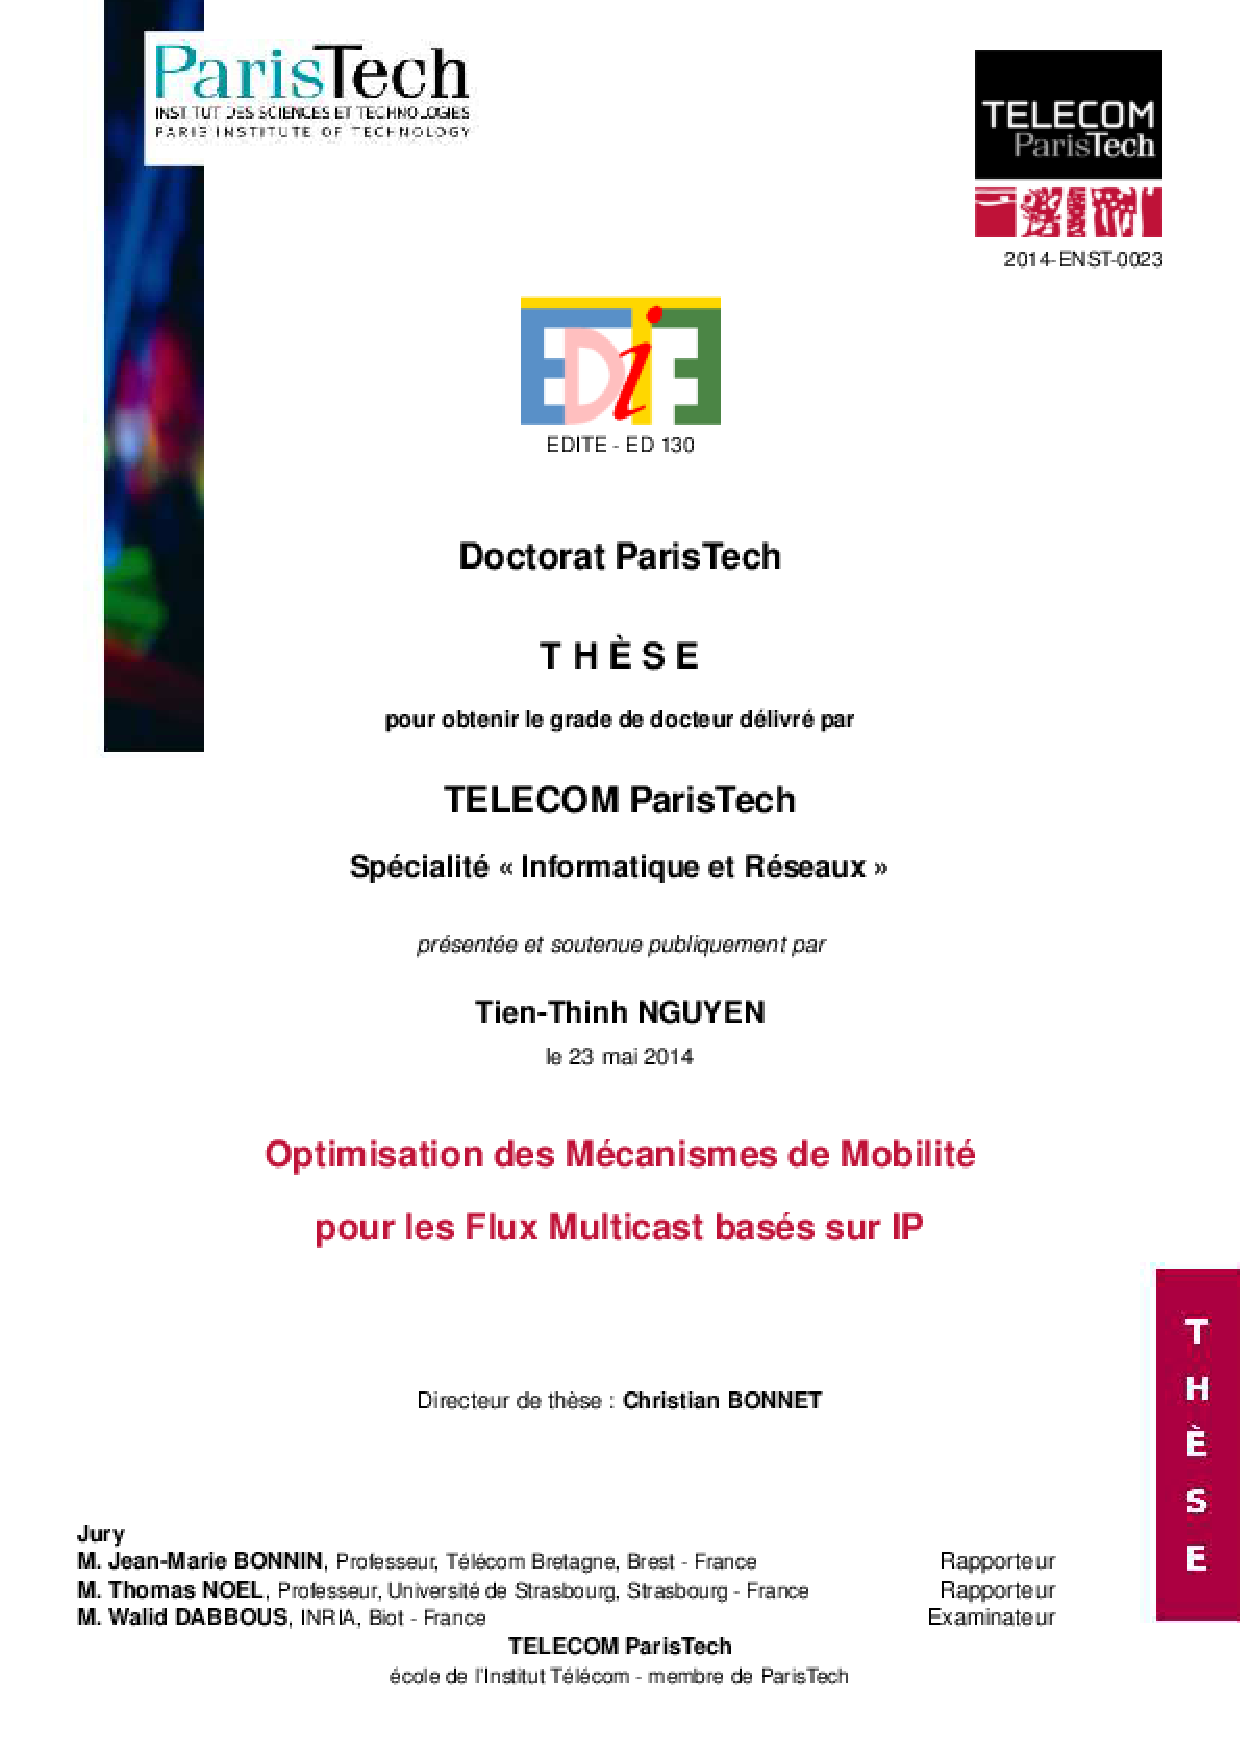
\includepdf[pages={1}]{TPT_Premiere.pdf}

  \vspace{10mm}
  \noindent




	\begin{center}
	
\includegraphics[width=48mm]{logo_ParisTech}
	\end{center}

  \vspace{5mm}


\center

\begin{bfseries}
  \noindent{\LARGE Optimization of Mobility Mechanisms 
\vspace{4mm}
  \\ for IP based Multicast Flows}
  \vspace{15mm}

  \noindent{\Large Tien-Thinh NGUYEN}
  \vspace{10mm}
\end{bfseries}


\noindent{A doctoral dissertation submitted to:}

\vspace{2mm}

\noindent{TELECOM ParisTech}

\vspace{2mm}

\noindent{In Partial Fulfillment of the Requirements for the Degree of:}

\vspace{2mm}

\noindent{\textbf{Doctor of Philosophy}}

\vspace{2mm}

\noindent{Specialty : \textsc{Computer Science and Networking}}

\vspace{2mm}




\vspace{6mm}

\noindent{ \large \textit{Thesis Supervisor:} ~~\textbf{Prof.\ Christian \textsc{Bonnet}}	}

\vspace{2mm}
 
 
\begin{center}
\noindent \large 
\begin{tabular}{llcl}
      \textit{Jury:}	& 		& & \\\\
     \textit{Reviewers:} & & & \\
 \multicolumn{2}{l}{~~\textbf{Prof.\ Thomas \textsc{Noel} }} 		& - & Universit\'{e} de Strasbourg, Strasbourg - France\\
 \multicolumn{2}{l}{~~\textbf{Prof.\ Jean-Marie \textsc{Bonnin}}} 		& - &  T\'{e}l\'{e}com Bretagne, Brest - France\\
\\
      \textit{Examiner:}& 		& & \\
      
\multicolumn{2}{l}{~~\textbf{Dr. \ Walid \textsc{Dabbous}}}           & - & INRIA, Biot - France\\
\\


  
\end{tabular}
\end{center}

\end{titlepage}

}


\cleardoublepage

\pagenumbering{gobble}
\vspace{10mm}

\hfill
  \noindent{
\vspace{4mm}}


\begin{center}
\noindent \large 
\vspace{32mm}
%\noindent{\textbf{To my wife and my little son - Bi}}
 \end{center}

\vspace{3cm}
\dominitoc
\pagenumbering{roman}
\cleardoublepage


%\section*{}
% \vspace{118ex}
% \begin{center}
% \copyright \hspace{1ex}2012\\Tien-Thinh NGUYEN\\ALL RIGHTS RESERVED
% \end{center}
% \cleardoublepage


\addcontentsline{toc}{section}{Acknowledgements}
\markboth{Acknowledgements}{Acknowledgements}
\chapter*{Acknowledgements}

First of all, I would like to extend my sincere thanks to my advisor Prof. Christian Bonnet for his valuable support and brilliant ideas. Throughout this thesis, he has always found the time for me to guide and encourage my research activities. I also very much appreciate his dynamism and his competences that made this thesis work a success. It has been my real pleasure to work with Christian. \\

I would also like to thank Prof. Jérôme Härri who helped me so much with his stimulating technical discussions and constructive publication reviewing. A special warm thank to my master advisor Michelle Wetterwald for her kindness and words of wisdom which facilitate not only my research but also my life.\\

I am grateful to the committee members of my jury, Prof. Jean-Marie Bonnin, Prof. Thomas Noël and M. Walid Dabbous for their valuable inputs and time spent reading this thesis. \\

I would like to express my appreciation to my colleagues and friends at Eurecom, for all the unforgettable enjoyable moments and their helps. I also wish to extend my warmest thanks to all my friends in France and Vietnam for all the wonderful time we spend together.\\

Finally, last but not least, I want to express my special gratitude to my parents, my wife and my son for their unconditional support, love and trust. They, together with another members in my big family, make my life full of kindness and happiness with their encouragement.\\

\addcontentsline{toc}{section}{Abstract}
\markboth{Abstract}{Abstract}
\chapter*{Abstract}
With the development of wireless access technology as well as the explosion of mobile devices (such as smartphones, tablets, and vehicles), the next generation mobile network is not only restricted to provide the traditional voice services but also the data services. Also, the increasing penetration of the mobile devices is generating a huge number of data traffic over mobile networks. In all-IP mobile networks, IP mobility management is a crucial concept to meet the demand of ubiquitous Internet connectivity as well as new service requirements such as seamless handover across heterogeneous networks, consistent quality of experience and stringent delay constraints. In this context, the scalability and bandwidth efficiency from the multicast routing make the IP multicast a valuable solution from the application point of view to deal with a huge number of traffic, particularly, in mobile environments where users usually share frequency bands and limited capacity. But one of the major challenges for the multicast support is when considering mobility. It comes from the fact that the multicast protocols were designed to support the stationary multicast parties. As such, it raises some issues as a result of the interaction of IP multicast and IP mobility protocols such as service interruption, packet loss, routing non-optimal, and packet duplication, etc. In fact, the conventional IP mobility management (e.g., Mobile IPv6 (MIPv6) and Proxy Mobile IPv6 (PMIPv6)) which leverages on the centralized mobility management approach, brings several issues for the network operator like inefficient use of network resources, poor performance, and scalability issues. The concept of Distributed Mobility Management (DMM) aims to tackle these issues and helps the mobile operators address the challenges created by rising mobile usage while enhancing the overall customer experience.\\

In this thesis, our main objective is to deal with the multicast mobility-related issues. The solutions are proposed in the context of the evolution of the current IP mobility management: from the host-based to the network-based, and also from the centralized to the distributed mobility management. In more details, for a single PMIPv6 domain, we introduce a method to reduce the service disruption and leave latency. We then present a solution from the load balancing point of view to address the service disruption and packet duplication issue. As DMM has not been standardized, we propose an inter-domain mobility solution, which can be considered as a step in the evolution from PMIP towards DMM. Finally, we converge to a final architecture in a DMM environment that can offer various benefits and address most of the multicast listener mobility-related issues. Throughout this thesis, a near-to-real testbed is used to achieve the realistic results.

\clearpage


\addcontentsline{toc}{section}{Contents}
\markboth{Contents}{Contents}

\tableofcontents
\clearpage

\addcontentsline{toc}{section}{List of Figures}
\listoffigures
\clearpage
\addcontentsline{toc}{section}{List of Tables}
\listoftables
\clearpage

%\printnomenclature
\addcontentsline{toc}{section}{Glossary}
\markboth{Glossary}{Glossary}
\chapter*{Glossary}
List of Abbreviations and Acronyms\\
\\
\begin{center}
\begin{longtable}{p{5cm}p{8.8cm}}
% % \hline
\textbf{3GPP} & 3rd Generation Partnership Project\\
\textbf{4G} & Fourth Generation\\
\textbf{AAA} & Authentication, Authorization and Accounting\\
\textbf{ALM} & Application-Layer Multicast\\
\textbf{ASM} & Any-Source Multicast\\
\textbf{aHMAR} & Anchor HMAR \\
\textbf{aNMAR} & Anchor NMAR\\
\textbf{AP} & Access Point\\
\textbf{AR} & Access Router\\
\textbf{A-LMA} & Anchor LMA\\
\textbf{A-AAA} & Anchor AAA\\
\textbf{A-MAG} & Anchor MAG\\
\textbf{BA} & Binding Acknowledgment\\
\textbf{BCE} & Binding Cache Entry\\
\textbf{BU} & Binding Update\\
\textbf{CBT} & Core Based Tree \\
\textbf{CDN} & Content Delivery Network\\
\textbf{cHMAR} & Current HMAR \\
\textbf{C-LBC} & Central Load Balancing Controller\\
\textbf{cMAR} & Current MAR\\
\textbf{CMD} & Centralized Mobility Database\\
\textbf{CMF} & Context Management Function\\
\textbf{cNMAR} & Current NMAR\\
\textbf{CN} & Corresponding Node\\
\textbf{CoA} & Care-of-Address\\
\textbf{COMMA} & Common MMA\\
\textbf{DHCP} & Dynamic Host Configuration Protocol\\
\textbf{DMM} & Distributed Mobility Management\\
\textbf{DMMA} & Dynamic Multicast Mobility Anchor\\
\textbf{DSMIPv6} & Dual Stack Mobile IPv6\\
\textbf{DR} & Designated Router\\
\textbf{DVMRP} & Distance Vector Multicast Routing Protocol \\
\textbf{D-GW} & Distributed Gateway\\
\textbf{eNB} & Evolved NodeB\\
\textbf{EPC} & Evolved Packet Core\\
\textbf{ETF} & Explicit Tracking Function\\
\textbf{EV} & Electric Vehicle\\
\textbf{EVCS} & Electric Vehicle Charging Service\\
\textbf{FA} & Foreign Agent\\
\textbf{FI} & Fairness Index\\
\textbf{FMIPv6} & Fast Mobile IPv6\\
\textbf{FPMIPv6} & Fast Handovers for PMIPv6\\
\textbf{GGSN} & Gateway GPRS Support Node\\
\textbf{GPRS} & General packet radio service\\
\textbf{G2V} & Grid-to-Vehicle\\
\textbf{HA} & Home Agent\\
\textbf{HMAR} & Host-based Mobile Access Router \\
\textbf{HMIPv6} & Hierarchical Mobile IPv6\\
\textbf{HeNB} & Home eNodeB\\
\textbf{HIP} & Host Identity Protocol \\
\textbf{HNP} & Home Network Prefix\\
\textbf{HoA} & Home Address\\
\textbf{HSPA} & High Speed Packet Access\\

\textbf{IANA} & Internet Assigned Number Authority \\
\textbf{ICMD} & Inter-Domain Centralized Mobility Database\\
\textbf{IETF} & Internet Engineering Task Force\\
\textbf{IGMP} & Internet Group Management Protocol\\
\textbf{IFOM} & IP Flow Mobility\\
\textbf{IMR} & Intersection Multicast Router\\
\textbf{IP} & Internet Protocol\\
\textbf{IPTV} & Internet Protocol Television\\

\textbf{L2} & Layer 2\\
\textbf{L3} & Layer 3\\
\textbf{LB} & Load Balancing\\
\textbf{LBC} & Load Balancing Controller\\
\textbf{LIPA} & Local IP Access \\
\textbf{LLQC} & Last Listener Query Count \\
\textbf{LLQT} & Last Listener Query Timer \\
\textbf{LMA} & Local Mobility Anchor\\
\textbf{LMD} & Localized Mobility Domain\\
\textbf{LTE} & Long Term Evolution\\
\textbf{L-GW} & Local Gateway\\
\textbf{MAC} & Media Access Control\\
\textbf{MAG} & Mobile Access Gateway\\
\textbf{MALI} & Multicast Address Listening Interval\\
\textbf{MANET} & Mobile Ad hoc Network \\
\textbf{MAP} & Mobility Anchor Point \\
\textbf{MAR} & Mobile Access Router \\
\textbf{MBMS} & Multicast/Broadcast Multimedia Service\\
\textbf{MBone} & Multicast Backbone\\
\textbf{MBSFN} & Multicast/Broadcast over a Single Frequency Network\\
\textbf{MCTF} & Multicast Context Transfer Function\\
\textbf{MC-Req} & Mobility Context Request \\
\textbf{MC-Res} & Mobility Context Response \\
\textbf{MFC} & Multicast Forwarding Cache \\
\textbf{MGMF} & Multicast Group Management Function \\
\textbf{MIH} & Media Independent Handover \\
\textbf{MIPv6} & Mobile IPv6\\
\textbf{MLD} & Multicast Listener Discovery\\
\textbf{MMA} & Multicast Mobility Anchor\\
\textbf{MMAP} & Multicast by Multicast Agent Protocol\\
\textbf{MMF} & Mobility Management Function \\
\textbf{MN} & Mobile Node\\
\textbf{MN-ID} & Mobile Node's Identifier\\
\textbf{MNP} & Mobile Network Prefix \\
\textbf{MoM} & Mobile Multicast Protocol \\
\textbf{MOR} & Mobile Router \\
\textbf{MOSPF} & Multicast Open Shortest Path First \\
\textbf{MPDSR} & Multicast Protocol With Dynamic Service Range  \\
\textbf{MR} & Multicast Router \\
\textbf{MRIB} & Multicast Routing Information Base \\
\textbf{MSDP} & Multicast Source Discovery Protocol \\
\textbf{MTMA} & Multicast Tree Mobility Anchor \\
\textbf{MUMO} & Multicast Mobility Management Module \\
\textbf{NAI} & Network Access Identifier\\
\textbf{ND} & Neighbor Discovery\\
\textbf{NetLMM} & Network-based Localized Mobility Management  \\
\textbf{NEMO} & Network Mobility\\
\textbf{NI} & Node Information\\
\textbf{NMAR} & Network-based DMM Access Router \\
\textbf{NS-3} & Network Simulator NS-3 \\

\textbf{PBA} & Proxy Binding Acknowledgment \\
\textbf{PBS} & Personal Broadcast Service \\
\textbf{PBU} & Proxy Binding Update\\
\textbf{P-GW} & Packet Data Network (PDN) Gateway\\
\textbf{PIM} & Protocol Independent Multicast\\
\textbf{PIM-DM} & Protocol Independent Multicast - Dense Mode\\
\textbf{PIM-SM} & Protocol Independent Multicast - Spare Mode\\
\textbf{PIM-SSM} & Protocol Independent Multicast - Source Specific Multicast\\
\textbf{pHMAR} & Previous HMAR \\
\textbf{PLC} & Power Line Communication \\
\textbf{pMAR} & Previous MAR\\
\textbf{PMIPv6} & Proxy Mobile IPv6\\
\textbf{pNMAR} & Previous NMAR\\
\textbf{Proxy-CoA} & Proxy Care-of-Address\\

\textbf{QI} & Query Interval\\
\textbf{QRI} & Query Response Interval\\

\textbf{RIB} & Routing Information Base\\
\textbf{RPF} & Reverse Path Forwarding\\
\textbf{RV} & Robustness Variable\\

\textbf{SDN} & Software Defined Networking\\
\textbf{SGSN} & Serving GPRS Support Node\\
\textbf{SIP} & Session Initiation Protocol\\
\textbf{SIPTO} & Selected IP Traffic Offload\\
\textbf{SMR} & Session-to-mobility Ratio \\
\textbf{SPT} & Shortest Path Tree \\
\textbf{SSM} & Source-Specific Multicast\\
\textbf{S-GW} & Serving Gateway\\
\textbf{S-AAA} & Serving AAA\\
\textbf{S-LMA} & Serving LMA\\
\textbf{S-MAG} & Serving MAG\\

\textbf{tLMA} & Target LMA\\
\textbf{TLV} & Type-length- vector\\
\textbf{tMAR} & Typical location MAR\\

\textbf{RA} & Router Advertisement \\
\textbf{RADIUS} & Remote Authentication Dial In User Service\\
\textbf{RAN} & Radio Access Network \\
\textbf{RBMoM} & Range-Based Mobile Multicast  \\
\textbf{RP} & Rendezvous-Point\\
\textbf{RPT} & Rendezvous-Point Tree\\
\textbf{RO} & Route Optimization\\
\textbf{RS} & Router Solicitation\\
\textbf{RTT} & Round-Trip Time\\

\textbf{UDP} & User Datagram Protocol \\
\textbf{UE} & User Equipment \\
\textbf{UGC} & User Generated Content \\
\textbf{UML} & User-Mode Linux\\
\textbf{UNP} & Update Notification Message\\
\textbf{V2G} & Vehicle-to-Grid\\
\textbf{VoIP} & Voice over IP\\
\textbf{WiMAX} & Worldwide Interoperability for Microwave Access\\

\end{longtable}
\end{center}

\clearpage

\mainmatter
\chapter{Introduction}
\label{intro}
\section{Motivation and Problem Statement}
With the development of wireless access technology as well as the explosion of mobile devices (such as smartphones and tablets), the next generation mobile network is not only restricted to provide the traditional voice services but also the data services. In other words, it is evolving towards all-IP systems. In fact, the mobile data services have become an essential part of many consumers' lives \cite{cisco_forecast,data_services}. So far, users are using their mobile devices not only for personal life but also for work on a regular basis \cite{cisco_service,morgan_stanley, mobile_2010}. As a result, the mobile data traffic has been almost doubled each year during the last few years\footnote{The increasing traffic is mainly driven by mobile video traffic} \cite{cisco_forecast, ericsson}. This trend is expected to continue in the upcoming years, especially with the deployment of fourth generation (4G) networks. Despite the increasing volume of traffic, the average revenue per user is falling fast \cite{mobile_europe}. In addition, in all-IP mobile networks as mobile nodes may frequently change their point of attachment to the IP network, IP mobility management is a crucial concept to meet the demand of ubiquitous Internet connectivity as well as new service requirements such as seamless handover across heterogeneous networks, consistent quality of experience and stringent delay constraints. Mobility can be handled at different layers of protocol stack ranging from the link layer to the application layer, however, most of these mobility management protocols are located at the network layer. Mobile IPv6 (MIPv6), the first mobility protocol standardized by the Internet Engineering Task Force (IETF) for IPv6 networks, maintains the mobile node (MN)'s reachability when it is away from home. It is done by relying on a central mobility, namely Home Agent (HA). However, in MIPv6, the MN needs to perform the mobility-related signaling, that means the MIPv6 protocol stack is required at the MN. It is the main obstacle of the deployment of MIPv6 in the real world. For this reason, Proxy Mobile IPv6 (PMIPv6), as a network-based mobility management, helps to avoid the additional deployment in the MN so that the MN can be kept simple. In other words, mobility can be transparently provided to all legacy MNs. \\

The mobile network operators are being challenged by the increase of mobile data traffic (especially the video traffic) and the new requirements e.g., providing connectivity anywhere and at anytime with consistency of user experience, while preserving the economics of their networks and creating new opportunities for revenue growth. Faced with these challenges, the operators are seeking for innovative solutions to improve their network performance and efficiency, as well as to reduce the costs expended on network operation and maintenance. Two major focuses are: i) increasing the capacity of wireless communication systems;  and ii) designing and implementing an efficient system to deliver the data. Regarding the first aspect, further dramatic increases in radio capacity of mobile broadband will come with the implementation of new wireless technologies such as Worldwide Interoperability for Microwave Access (WiMAX), High Speed Packet Access (HSPA) and Long Term Evolution (LTE). However, spectrum for operators is both limited and expensive. Thus, they are looking at different methods to increase the system capacity such as deploying femto and pico cells, together with selecting the offload traffic between the licensed and unlicensed spectrum (e.g., from 3G to WiFi). Considering the second aspect, the aim is to simplify the network architecture as well as optimize the data transmission costs. Accordingly, the mobile network is currently evolving towards flat architecture. One example is Local IP Access/Selected IP Traffic Offload (LIPA/SIPTO) architecture defined by the 3rd Generation Partnership Project (3GPP). Following the same idea, IETF has recently chartered the Distributed Mobility Management (DMM) working group which specifies the solutions to address the problems and limitations of the current centralized mobility management. In fact, the conventional IP mobility management (e.g., MIPv6 and PMIPv6) leverages on the centralized mobility management approach, thus,  raises several issues for the network operators like inefficient use of network resources, poor performance, and scalability issues when considering a large number of mobile devices and their traffic demand \cite{DMM_requirements, DMM_issues,DMM_problem_statement}. DMM is one of the solutions to help the mobile operators address these limitations while enhancing the overall customer experience.  \\


As Internet is widely deployed and spread across a large area, it carries a variety of common information resources and services. In a sharing world, the group communication service, which refers to the ability to send data to several receivers at the same time, is naturally becoming more and more important especially in some areas like multimedia distribution, gaming, and financial services, etc. In this context, the scalability and bandwidth efficiency from the multicast routing make the IP multicast a remarkable solution from the application point of view to allow the mobile networks to deal with a huge number of traffic, particularly, in mobile environments where users usually share frequency bands and limited capacity \cite{Multicast_MIPv6}. But one of the major challenges for multicast support is when mobility is considered. It comes from the fact that the multicast protocols were designed to support the stationary multicast parties. As such, it raises some issues as a result of the interaction of IP multicast and IP mobility protocols e.g., transparency, routing optimization, packet duplication, service disruption, packet loss and group leave latency, etc \cite{Multicast_MIPv6, multicast_challenges_solutions}.\\
 
Regarding the IP mobile multicast, after more than a decade of research and development efforts, many approaches have been proposed, but most of them are based on such host-based mobility management protocols as MIPv6, Fast Mobile IPv6 (FMIPv6) and Hierarchical Mobile IPv6 (HMIPv6). However, the main drawback of these protocols is that they require the MN to modify its IP stack to participate into the mobility signaling process. In fact, it is the major obstacle of the deployment of MIPv6 in the real world. Additionally, the previous IP multicast approaches cannot be directly applied in a network-based mobility management in which the MN is unaware of mobility process. To solve the aforementioned issues, the IETF has worked in different solutions highlighting the difference between the source and the listener multicast mobility problems in PMIPv6. However the proposed solutions remain unable to address the issues of scalability, performance optimization and compatibility with unicast mobility at the same time. In DMM, there is no complete solution for the multicast mobility support.\\

It is generally acknowledged that a proposed solution cannot be widely accepted without results from valid experimentation. Such validation nowadays can be obtained through various methods, each with its own advantages and limitations. Within the networking field of research, the results’ reliability is one of the most critical issues. Thus, the results credibility is directly related to the methods used, therefore improving them becomes of great importance. In this context, the most widely used method - simulation - sometimes lacks credibility. The lesser used but most credible method - real testbed - is too expensive and difficult to scale and manage. \\

In this thesis, our objective is to deal with the multicast-related issues raised when a multicast node moves in a network-based mobility management domain. In other words, the aim of this research is to find solutions that ensure:
\begin{itemize}
\item Keeping the MN unaware of mobility from the multicast service point of view;
\item Minimizing the service disruption time to even satisfy the strict requirements for the interruption- and delay-sensitive services;
\item Keeping the signaling/tunneling overhead as low as possible;
\item Maximizing the available network resource (reducing the waste of resources and packet duplication), keeping the reliability and improving the scalability of the system;
\item Minimizing the modifications of the mobility management and the multicast routing protocols to support IP mobile multicast. 
\end{itemize}
\begin{figure}[h!] 
 \begin{center} 
 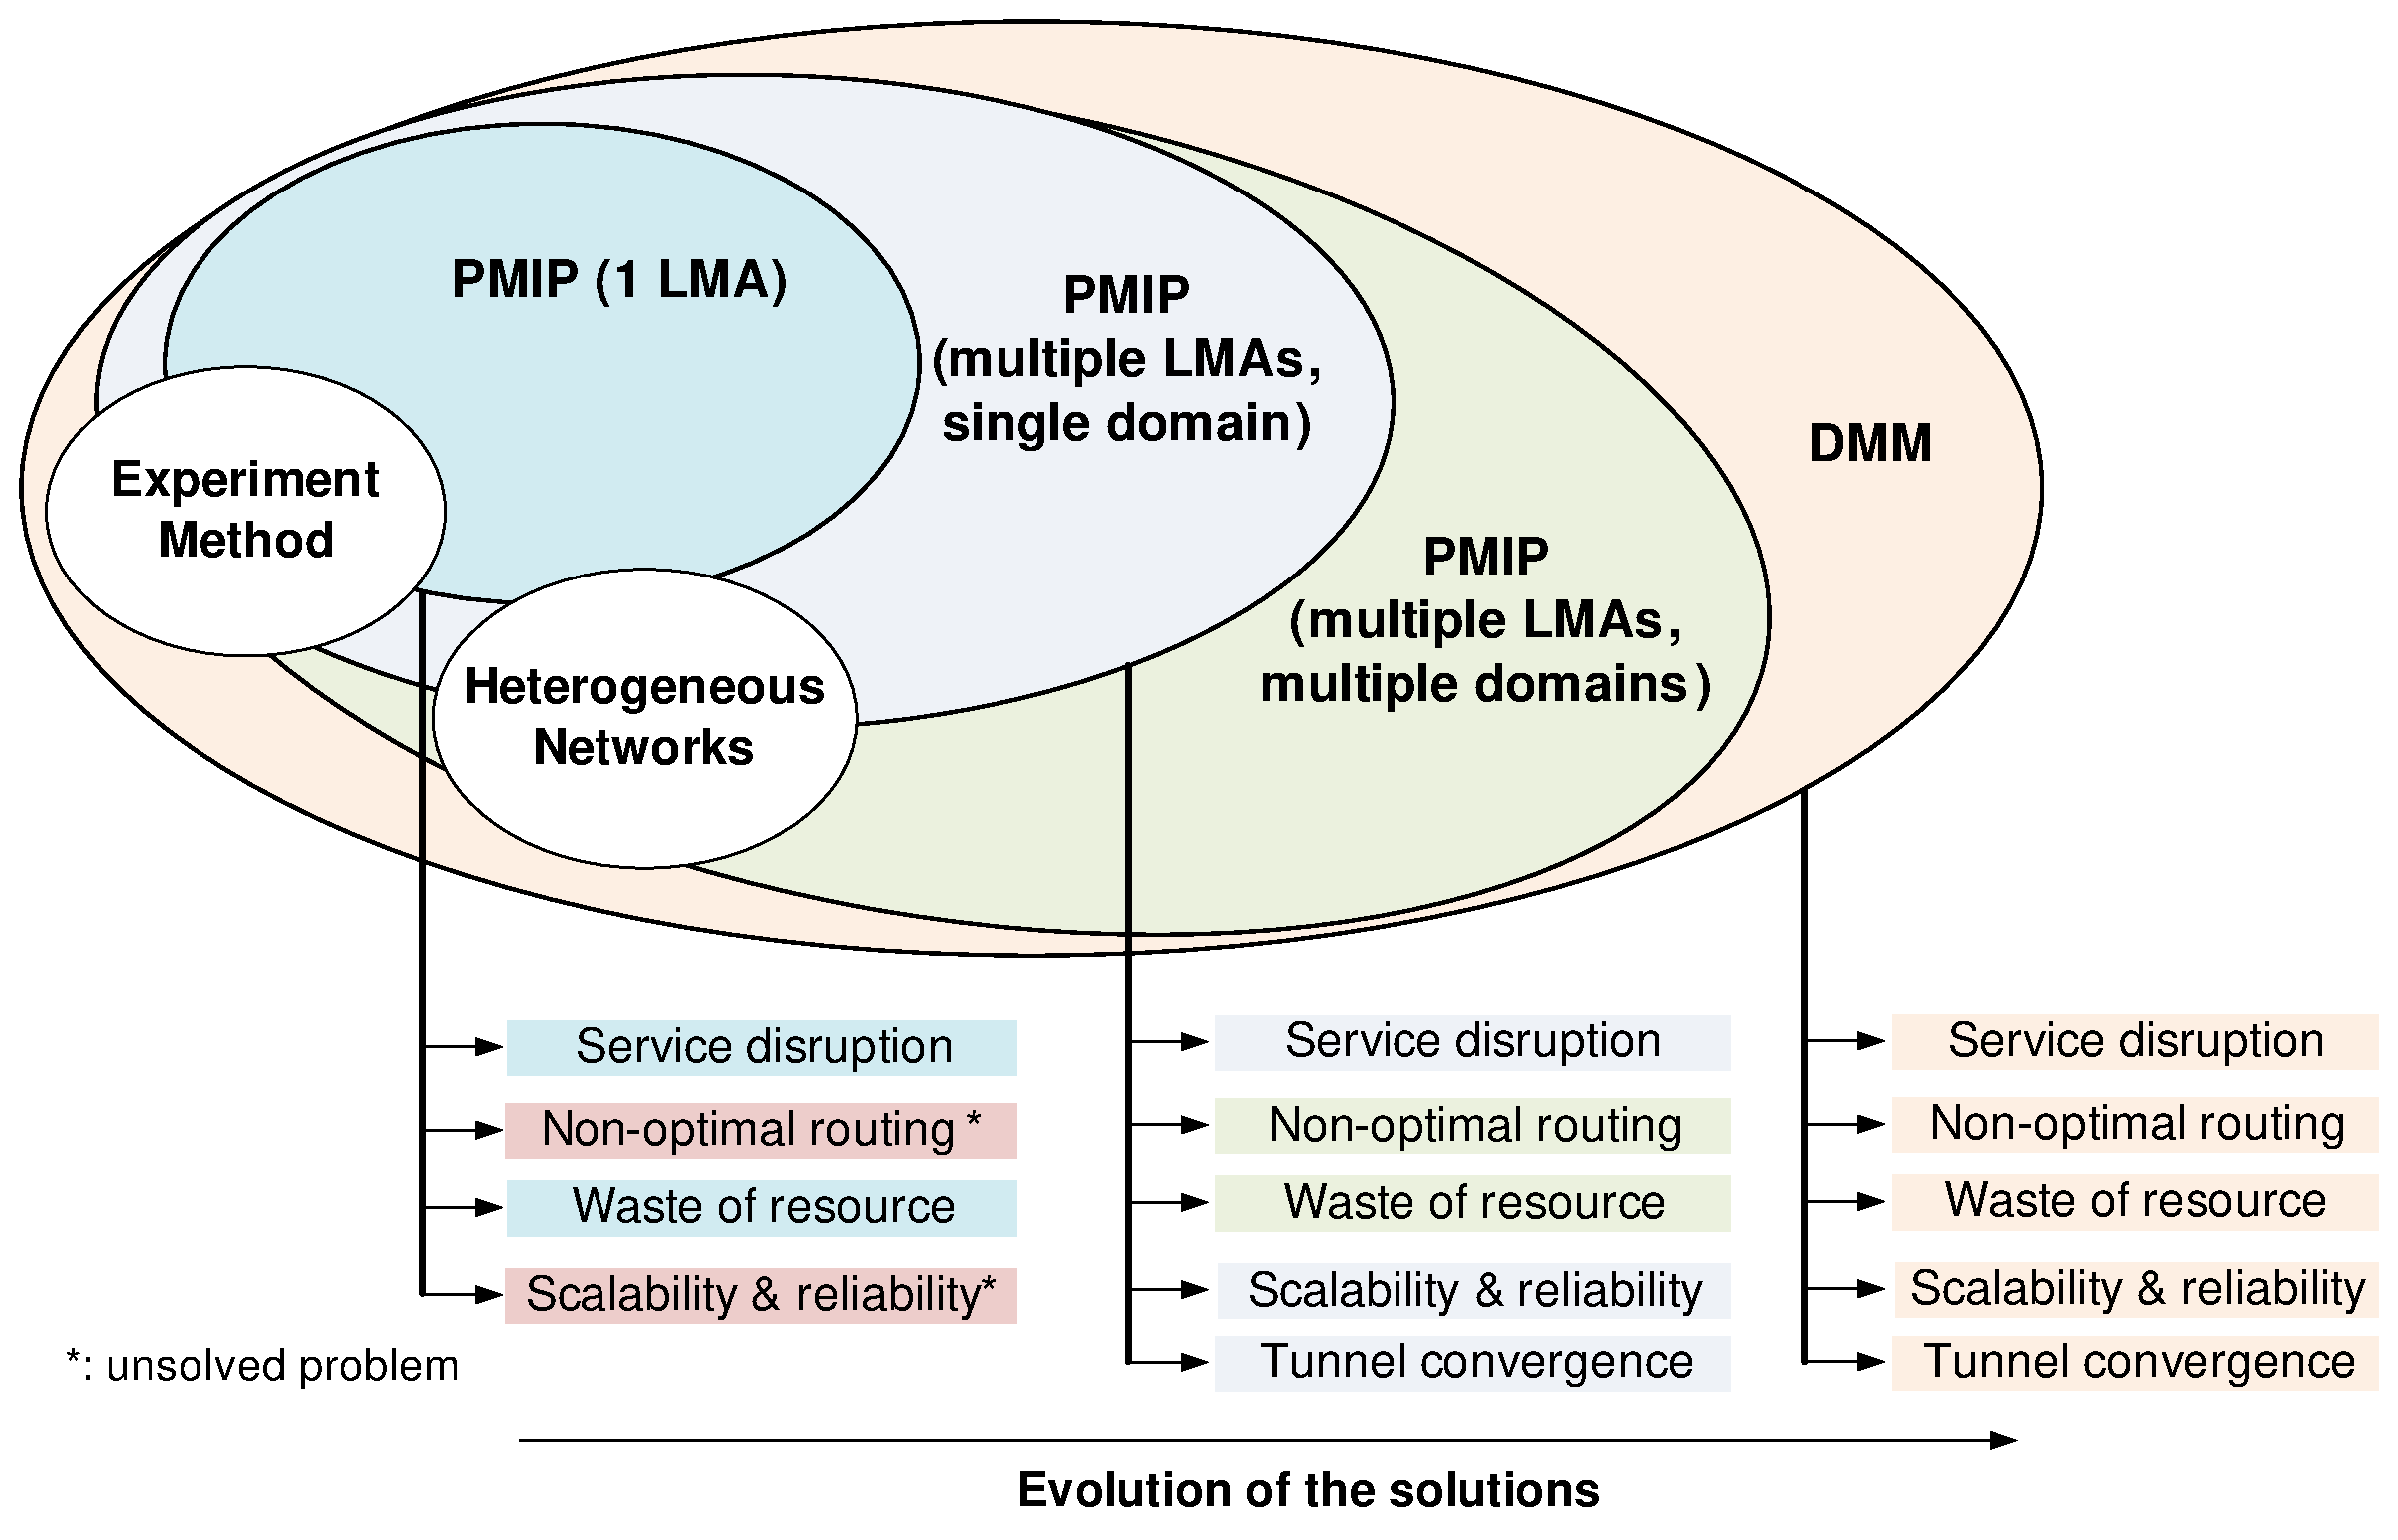
\includegraphics[width=0.72\textwidth]{./Introduction/Chapter1/figures/vision.eps} 
    \caption{Evolution of the solutions for multicast mobility.}
     \label{fig:vision}
  \end{center} 
\end{figure}
The evolution of the solutions for multicast mobility is illustrated in Fig.~\ref{fig:vision}. For a single PMIPv6 domain (with one local mobility anchor (LMA)), we introduce a method to minimize the service disruption time considering both cases: a mobile node with single or multiple interfaces. The waste of resources caused by a long leave latency is also reduced. On the other hand, the non-optimal routing; scalability and reliability issues are unsolved. Considering a single PMIPv6 domain with multiple LMAs, an additional issue is introduced - the tunnel convergence problem (or packet duplication). To improve the scalability and reliability for PMIPv6 network while addressing the tunnel convergence problem, the load balancing mechanism is proposed at an acceptable cost of service disruption. As DMM is still under discussion and has not been standardized, we provide an inter-domain mobility support which can be considered as a step towards the deployment of DMM. IP multicast then will be considered in both the inter-domain and the DMM environments. Taking benefits of the previous proposed solutions, the dynamic multicast mobility anchor (DMMA) mechanism in DMM addresses almost all the multicast mobility-related issues such as service disruption, non-optimal routing, waste of resources, tunnel convergence and scalability. Additionally, throughout our thesis, a near-to-real testbed will be used to achieve the realistic results. 

\section{Thesis Contributions and Outline}
The key contributions to the study of IP mobile multicast proposed in this thesis can be summarized as follows.
\paragraph{PMIP-based solutions}
\begin{itemize}
\item \textit{A method to minimize the multicast service disruption time during handovers inside a PMIPv6 domain}: This solution is based on the multicast context transfer and the explicit tracking function. Then, a PMIPv6 testbed has been deployed, which allows simulating the mobility of multiple multicast sources and listeners at the same time. A real implementation of the multicast context transfer function and the explicit tracking function has been deployed. Also, the listener part of Multicast Listener Discovery Version 2 (MLDv2) has been developed in NS-3.

\item \textit{A multicast-based load balancing mechanism among LMAs to solve the problem of bottleneck and single point of failure at the LMA}: This mechanism taking multicast into account helps to better distribute the load caused by the multicast flows in a PMIPv6 domain. Also, this solution can co-operate with the existing load balancing mechanisms to enhance the scalability and reliability of the system. 

\item \textit{Mobility in heterogeneous networks discussions via a use case: electric vehicle charging service (ECVS)}: By using PMIPv6, the service takes care of the Electric Vehicle (EV) mobility, handling vertical and horizontal handovers between different communication technologies (e.g., Wireless LAN (WLAN), LTE and Power Line Communication (PLC)). The IPv6 address preservation in PMIPv6 is guaranteed by relying on the logical interface mechanism which helps to hide the change of interface to the IPv6 stack. Moreover, the logical interface keeps the MN unaware of the interface change as well as mitigates its impact on the service disruption. 
\end{itemize}

\paragraph{DMM-based solutions}
\begin{itemize}
\item \textit{A solution for inter-domain mobility for PMIPv6}: It allows the data packets to be routed via a near-optimal way by bringing the mobility anchors closer to the MN while the control management can be placed anywhere in the network. This solution can be considered as a one step towards the deployment of DMM. A basic support for the multicast listener mobility in an inter-domain environment then is provided.  

\item \textit{A dynamic multicast mobility anchor selection in DMM (DMMA)}: It enables a per-flow multicast support. From a multicast service perspective, it helps satisfy the requirements in terms of service disruption and delay, especially when considering the real-time services. The packet duplication and waste of resources (or leave latency) issues can be reduced. Also, it provides a mechanism to better distribute the load among the Mobile Access Routers (MAR). The DMMA mechanism takes the advantages from the previous contributions into account, for example: i) the multicast context transfer and explicit tracking function are re-used to minimize the service disruption; ii) the load information is used as a metric for the multicast anchor selection; iii) the method of load collection is applied to collect others metrics; and iv) the operation of the central mobility database (CMD) is similar to the inter-domain central mobility database from the inter-domain PMIPv6 proposal. 
\end{itemize}

In order to validate the solutions with a high degree of confidence, \textit{an experiment method is used to achieve the realistic results at low cost}. This is a trade off between the simulation method which in some cases lacks of credibility and the real testbed which is typically too expensive, difficult to scale and manage. Based on this method, a testbed is deployed to conduct the experiments for the multicast mobility in PMIPv6. Additionally, this method can be generally applied for the experimentation in wireless mobile networks.  \\

The work presented in this thesis is structured as follows. A part from the introduction and final conclusion, we divide the content of the thesis into three main parts. We present a brief description of the related works in the first part. Then, in part II and III, we discuss the solutions for the mobile multicast-related issues.

\begin{enumerate}
\item In the first part, we provide an overview of IP multicast and IP mobility. This part also highlights the issues and challenges when considering multicast in a mobile environment. Particularly, we make a brief introduction of the main approaches proposed by the IETF regarding their advantages and limitations. Based on this analysis, the solutions for the remained issues will be presented in the next parts. Also, we enlist the requirements for an effective performance evaluation of mobile multicast solution. We then propose an efficient method for experimentation in the wireless mobile networks. The testbed, which is developed based on this method, will be used throughout this thesis to validate the solutions. 

Results have been presented and / or published
\begin{enumerate}
\item in the Future Network and Mobile Summit (Futurenet 2012) \cite{Thinh_futurenet}
\item within an official research deliverable of Medieval \cite{d4.2, d4.3}
\end{enumerate}

\item The second part discusses several issues when a multicast node moves in a single PMIPv6 domain. Chapter \ref{ch:multicast_PMIP} focuses on the service disruption issue. Chapter \ref{ch:LB} proposes a load balancing mechanism taking multicast service into account to better distribute the load among LMAs, so as to improve the scalability and the reliability of the PMIPv6 domain. Chapter \ref{ch:EVCS} discusses the mobility of a multihomed node in which the logical interface mechanism is used to hide the change of physical interface to the IP stack.

Results have been presented and / or published
\begin{enumerate}
\item at the Wireless Communication and Networking Conference (WCNC 2013) \cite{Thinh_WCNC_Multicast}
\item at the 24th Annual IEEE International Symposium on Personal, Indoor and Mobile Radio Communications (PIMRC 2013) \cite{PMIP_EV}
\item at the CNC workshop, 2014 International Conference on Computing, Networking and Communications (ICNC 2014) \cite{Thinh_ICNC}
\end{enumerate}

\item In the last part, we first propose an inter-domain mobility support for PMIPv6 based on the DMM concept in Chapter \ref{ch:inter_domain}. Then in Chapter \ref{ch:multicast_dmm}, we propose a dynamic multicast mobility anchor selection in DMM which enables a per-multicast flow support. The proposed mechanism helps satisfy the requirements in terms of service disruption and delay, especially when considering real-time services. Also, it provides a mechanism to better distribute the load among the MARs. 

Results have been presented and / or published
\begin{enumerate}
\item at the International Conference on Communications (ICC 2014) \cite{Thinh_ICC}
\item at the 78th Vehicular Technology Conference (VTC2103-Fall) \cite{Thinh_VTC}
\item at the Wireless Communication and Networking Conference (WCNC 2013) \cite{Thinh_WCNC_DMM}
\item at the 9th International Conference on Networking and Services \cite{Thinh_ICNS}
\item at the International Conference on Communications (ICC 2013) \cite{ICC_Sergio}
\end{enumerate}
\end{enumerate}

The contributions of this thesis have also been submitted to the Computer Networks journal, Elsevier \cite{Thinh_elsevier_LB} and will be submitted to the Wireless Networks journal, Springer \cite{Thinh_Springer}.





\part{Background Analysis\label{pa:part1}}

\chapter*{Overview of Part \ref{pa:part1}}
In this Part, we will introduce the fundamental notions of IP multicast, mobility management protocol as well as identify the issues and challenges when considering multicast in wireless mobile networks. We then enlist the performance evaluation metrics for IP mobile multicast. Next, we present an experiment testbed for IP mobile multicast which provides realistic results at a low cost. More than that, our experiment method in general can be applied for experiment in wireless mobile networks. \\

In Chapter \ref{ch:reference_technologies}, we describe the basic notions of IP multicast, its components and its applications in the Internet. To deploy the multicast service, two fundamental components are needed: group management protocols and multicast routing protocols. We then present in details of how an IP multicast service works from the Protocol Independent Multicast - Sparse-Mode (PIM-SM) and MLD protocols point of view. Regarding the IP mobility management protocols, starting from MIPv6 and its variants, we introduce PMIPv6 protocol and its enhancements. After discussing the limitations of the centralized mobility management such as MIPv6 and PMIPv6, DMM will be presented as a promising mobility management scheme for future networks. Based on the fundamental concepts of IP multicast and mobility management protocols, we highlight the issues and challenges when applying IP multicast in a mobile environment. Different impact factors on the multicast service are identified. At the end of this chapter, we highlight such issues as multicast service disruption time, packet loss, tunnel convergence problem, sub-optimal routing, end-to-end delay, and leave latency (waste of resources). \\

In Chapter \ref{ch:performance_evaluation}, a list of specific requirements that would lead to the design of the target solutions is provided. We then define the performance metrics that are crucial to access the effectiveness of a mobile multicast solution. In the context of this thesis, we focus on such metrics as signaling overhead, handover latency (multicast service disruption time), end-to-end delay, packet loss and tunneling overhead. The qualitative metrics like easy-to-deploy and scalability are also taken into account. We then introduce an experiment method which in some cases is used to improve the degree of confidence of the solution's results. Additionally, it can be considered as a framework that aims to close the gap between research experimentation and real deployment. \\

Throughout this thesis, in order to validate the results, firstly, we use an analytical analysis. The proposed experiment method then, in some cases, is used to improve the degree of confidence of the results.

\chapter{Reference Technologies and Challenges}
\label{ch:reference_technologies}
\section{Overview Internet of Things and Related Concepts }
\subsection{Internet of Things}
The concept of Internet of Things was first coined by Kevin Ashton, Executive Director of the Auto-ID Center in Massachute Institute of Technology (MIT) in 1999, and it is described as a world where billions of objects can sense, communicate and share information \cite{madakam2015internet}. Then IoT becomes more popular due to the explosion of mobile devices, ubiquitous communication, cloud computing. However, the definition of ``Internet of Things'' is still ambiguous, and have different facets depending on the perspective. From the view of functionality and identity, IoT is defined as ``Things having identities and virtual personalities operating in smart space using intelligent interfaces to connect and communicate within the social, environmental, and user contexts'' \cite{ray2018survey}. Semantically, the term of Internet of Things is composed of two words ``Internet'' and ``Things''. Following this way, IoT could be defined as ``a worldwide network of interconnected object uniquely addressable, based on standard communication protocols''~\cite{minerva2015towards}.\\

Similar to its definition, the characteristic of IoT vary from one domain to another. Some of the key characteristics identified during the research study are as follows:
\begin{itemize}
    \item \textbf{Dynamic and Self-adapting}: IoT devices and system must be able to dynamically adapt with the changing contexts or sensed environment. For example: considering a smart building system comprising of a number of temperature devices. These devices can adapt their modes based on whether it is indoor or outdoor. Based on that, they can adjust the calibrations to collect data more accurately. In this example, the smart building system is adapting itself with the change of context or environment.
    
    \item \textbf{Self-configuring}: IoT device may have the capability to configure themselves relating connection, software upgrades, etc., while minimal user intervention.  This characteristic allows co-operating a large number of devices to provide specific functionality.
    
    \item \textbf{Interoperable Communication Protocols}: The IoT devices may support multiple connectivity (Wifi, Lora, Sigfox, etc.) to communicate with other devices as well as the cloud infrastructure.
    
    \item \textbf{Unique Identify}: IoT device must be identified by a unique identity (such as an IP address or an URL). In addition, the IoT system needs to provide intelligent interface allowing the end-user to access directly these devices.
    
    \item \textbf{Integrated into Information Network}: In order to communicate and exchange data, IoT devices are integrated into the information network. In addition, these devices can be dynamically described and discovered in the network by other IoT devices or systems. For example A weather station can describe its monitoring information to other station in the same information network so that they can communicate and exchange collected data. Such integration could enrich the acquired information because of the data aggregation from several nodes.
    
\end{itemize}

\subsection{Web of Things and Semantic Web of Things}
Recent years, we have been witnessing the explosion of Internet of Things in term of the number and types of IoT devices. Unfortunately, there is no universal application protocol that is compatible with various networking interface. Thus, building a single global ecosystem of Things communicating with each other seamlessly is still impossible~\cite{WebofThi19:online}. In other words, the IoT is a collection of ``Silos of Things'' that can not interact with each other. Therefore, to build a global Internet of Things, we need a universal language and protocols supporting the interaction between devices and application regardless their properties (types, firmware, configuration, etc.). Instead of inventing a dedicated technology, leveraging the widely popular web protocols, standards, and blueprints to make data and services offered by Things more accessible to a larger pool of developer~\cite{guinard2016building}. That is premise behind adoption of the Web of Things. The ultimate goal of Web of things is effectively breaking the ``Silos of Things'' also known as ``one device, one protocol, one app'' by applying tools and techniques that are available on the Web technology.

In order to archive its goals, WoT is used on the Application level to abstract the complexity and variety of lower-level (protocols, firmware, data formats, etc.) by a simple Web model to facilitate the integration of all IoT devices and application. In other words, by hiding the heterogeneity of IoT devices and application behind Web technologies, the WoT allows developers to focus on their application without considering the technologies behind. In practice, the developers could interact with IoT Things via web browsers and explore the Things as surfing the web. The collected data from Things is visually displayed using Web programming language such as HTML, CSS, and Javascript. 

In general, the Web of Things facilitates the interaction and exchange of information between different Things and System powered by Web technologies. However, the exchanged data can be encoded and presented under different formats (envelopes, semantics, and meta-data) . For example, the collected data presenting current temperature can be under plain text, XML/EXI, or JSON format. The file name can be ``temperature'' or ``temp''. Therefore, it is necessary to build a Semantic Web of Things (SWoT) to ensure a common understanding and format. In other words, SWoT concept is the evolution of the Web on Things with the Semantic technology. The goal of SWoT is to provide comprehensive interoperability that allows not only sharing and reuse of IoT Things but also making IoT data to be universally understandable~\cite{pfisterer2011spitfire}. The summary of evolution from Internet of Things to Web of Things is illustrated in Figure~\ref{fig:c2_evolution_iot_swot}

\begin{figure}[h!] 
 \begin{center} 
 \includegraphics[width=0.72\textwidth]{./Part1/Chapter2/figures/c3_evolution_iot_swot.jpg} 
    \caption{Evolution of the solutions for multicast mobility.~\cite{jara2014semantic}}
     \label{fig:c2_evolution_iot_swot}
  \end{center} 
\end{figure}

\subsection{Massive Internet of Things}
With the explosion of Internet of Things, the number of Things and its connectivity have been growing exponentially. In addition, Things is no longer just send the data to cloud, but also exchange information to each other. As a result, Massive IoT is emerging as a new focal point for IoT connectivity technologies referring to huge volume of constrained IoT devices, which stringently require excellent coverage, cost-effective and low-energy consumption~\cite{Northstream2017}. Among several new connectivity technologies for MIoT, proprietary LPWAN technologies such as Sigfox and LoRA have been considering the most potential candidates while cellular-based connectives such as 5G or NB-IoT are under developing and testing process \cite{raza2017low}.

On a technical level, the IoT devices in Massive Internet of Things context are distributed in a wide area from large manufacturing plants to inside sewer systems where the radio signal is physically challenging. To adapt to such environments, the connectivity technology of Massive IoT is not only wide coverage but also robust. In addition, replacing device battery in large area is very expensive. This connectivity technology must be low energy consumption to extend the device battery life. Typically, high throughput and latency are not unessential in massive IoT applications, since they more focus on collecting data than controlling.


\section{Fundamentals of IoT}
\subsection{IoT Things}
Similar to Internet of Things definition, deriving a unified definition for the ``Things’’ in IoT is still challenging although it has received most attention from academic organizations such as NIST, ITU, W3C, IERC, and IETF~\cite{Liu2016}. IEEE simply defined the Things as a physical object that is relevant from a user or application perspective~\cite{minerva2015towards}. However, IERC believes that a Thing can be physical or virtual and identified by unique identity~\cite{smith2012internet}. NIST proposes the Things can be all software, all hardware, or the combination of software and hardware.~\cite{voas2016networks}. 

Due to the heterogeneity in Things definition, we simplify the Thing could be physical or virtual object integrated into a network. This object can interact via a unique identity and intelligent interface. For example, a smart phone can be a Thing which is physical object, able to join networks (WiFi, cellular network), has unique identity (phone number, IP address) and intelligent interface. A database is also considered as a Thing because it is a virtual object, able to join networks (internet), has unique identity (URL) and intelligent interface (Web services).
\subsection{IoT Connectivity}
In this section, rather than mentioning all the IoT protocol following existing architecture model like OSI models, we only present some dedicated protocols in IoT and organize them based on their functionality.

\begin{description}
\item[\textbf{Infrastructure}:\\]
    \begin{itemize}
    \item[] 
    \item \textit{6LoWPAN: } This is an acronym of IPv6 over Low Power Wireless Personal Area Networks defined by the Internet Engineering Task Force, IETF in their document RFC 6282~\cite{shelby20116lowpan} deriving from the idea that "the Internet Protocol could and should be applied even to the smallest devices,"~\cite{Mulligan:2007:ARC:1278972.1278992}. This protocol uses 2.4 GHz frequency with 250 kbps rate.
    
    \item \textit{uIP: } The uIP is an open source project licensed under a BDS style license~\cite{adamdunk86:online}. The goal of this project is to create a dedicated TCP/IP stack for 8 or 16 bits micro-controllers. Currently, it is further developed by wide community.
    
    \item \textit{NanoIP: } The concept NanoIP is to optimize all features of Internet to adapt to embedded and small devices, without the overhead of TCP/IP~\cite{shelby2003nanoip}.NanoIP uses two dedicated transport techniques are nanoUPD and nanoTCP. A socket-compatible API is also provided to make sure the protocol similar to original IP protocol.
    
    \item \textit{Time Synchronized Mesh Protocol (TSMP): } TSMP is a communication protocol designed for self-origanizing network of wireless devices enabling reliable, low power, secure communication~\cite{pister2008tsmp} 
    
    \end{itemize}

\item[\textbf{Discovery}:\\]
    \begin{itemize}
    \item[] 
    \item \textit{mDNS: } The mDNS is used to resolves host names to IP addresses within small networks. Except do not include a local name server,  this technology is essentially the same with the unicast Domain Name System (DNS) in term of programming interfaces, packet formats and operation~\cite{cheshire2013multicast}. 
    \item \textit{Physical Web: } The Physical Web aims to discover and interact with nearby devices through a list of URLs being broadcast. That means every smart object in the network needs to broadcast its access URL that any nearby device can receive. 
    \item \textit{HyperCat: } HyperCat is an open, lightweight JSON-based hypermedia catalogue format to exploit Thing resources~\cite{HyperCat76:online}. It allows adding a set of semantic annotations to Things resources and make them discoverable over the web. 
    \item \textit{Universal Plug and Play (UPnP): } The UPnP uses Internet and Web protocols to automatically discover new devices to be plugged into a network. These new devices announce their presence to other devices by using a discovery protocol based on HTTP~\cite{RFC6970U68:online}. 
    
    
    \end{itemize}

\item[\textbf{Data Protocol}:\\]
    \begin{itemize}
    \item[] 
    \item \textit{Message Queuing Telemetry Transport (MQTT): } MQTT \index{MQTT} is an publish-subscribe based messaging protocol working on the top of TCP/IP protocol. It is useful for connections limited bandwidth~\cite{}. An MQTT system consist of a central messaging server named "message broker" and clients. There are two client types are: (1) publisher: clients publish data to broker. (2) Subscriber: Clients receive data from broker. The responsibility of broker is to forward data from publishers to subscribers. 
    
    \item \textit{Constrained Application Protocol (CoAP): } CoAP \index{CoAP} is an application layer protocol designed for constrained internet devices that are limited in storage, computation power. It is based on RESTful protocol design to simply translate to HTTP for simplified integration, while also meeting specialized requirements such as multicast support, very low overhead, and simplicity~\cite{RFC7252T93:online}. Currently, the major standardization for CoAP is done by The Internet Engineering Task Force (IETF) and various new functionalities have been added~\cite{colitti2011integrating}. 
    
    \item \textit{Extensible Messaging and Presence Protocol (XMPP): } XMPP \index{XMPP} is a real-time communication protocol based n Extensible Markup Language (XML). It is defined in an open standard managed by The Internet Engineering Task Force (IETF). Dsigned to be extensible, the protocol is also used for publish-subscribe model in VoIP~\index{VoIP}, video and IoT application \index{IoT!application}. 
    
    \item \textit{Advanced Message Queuing Protocol (AMQP): } Similar to XMPP\index{XMPP}, AMQP is an open standard application layer but it is designed for message-oriented middleware. Thereby, its functionalities ensure reliability and security such as message orientation, queuing, routing~\cite{o2007toward}. The authentication and encryotion based on Simple Authentication and Security Layer(SASL)\index{SASL} or Transport Layer Security (TLS)\index{SASL}
    
    \end{itemize}
    
\end{description}

\subsection{IoT Middleware}
\subsection{IoT Applications}
\section{IoT Cloud}
\subsection{Foundation for IoT Framework}
\subsection{IoT Cloud Requirements and Challenges}
\subsection{Cloud-based IoT Platforms and services}
\section{Interoperability in IoT Cloud}
\subsection{Interoperability why, where and how}
\subsection{Interoperability challenges}
\section{Reliability in IoT}
\subsection{Data Reliability}
\subsection{Device Reliability}
\section{Conclusion}
 

\chapter{Performance Evaluation for IP Mobile Multicast}
\label{ch:performance_evaluation}
\section{Interoperation in IoT}
\subsection{Related works}

To increase the interoperability in IoT, researchers have leveraged several approaches and technologies from other fields such as semantic, cloud computing, fog computing, etc. In this section, we present an overview of current approaches as well as challenges to achieve interoperability. For each proposal, we examine its interoperability level (technical, syntactical, semantic and organizational interoperability), openness, and security perspectives.

\subsubsection{Adapters/gateways}

Gateways or adapters are the class of schemes aiming to improve interoperability between IoT devices. This approach uses an intermediate tool called mediator installed in IoT gateways or adapters to converse protocols, data, standards between sending and receiving devices. For instance, an IoT device using Bluetooth connectivity desires connecting to other devices using ZigBee connectivity. In such context, gateway can be installed dedicated hardware or software which could converse Bluetooth connectivity to ZigBee connectivity and vice versa.\\

The most critical challenge of this approach in scalability. With a large number of heterogeneous IoT devices, it demands considerable efforts to design specific connectors. In addition, the performance of conversion must be considered. For example, if the system needs to support n connectivity, we have to develop $\frac{n*(n-1)}{2}$ connectors. These connectors cannot be implemented in a single gateway. Therefore, several one-to-many protocol gateways solution is used. \\

Several proposals in both academic and industrial focus on designing and standardizing IoT gateway. Ponte~\cite{PonteM2M76:online} presents a framework enabling data exchange between various IoT devices through different connectors. The main limitation of this framework is that it only supports HTTP, CoAP, and MQTT, which are incompatible with resource-constrained devices. In addition, developing a new connector is extremely complex works. Zhu et al.~\cite{zhu2010iot} propose an IoT gateway architecture using user-space programmable software to interoperate between wireless sensor network (WSN)\index{WSN} protocols and mobile communication networks or Internet. Such gateway supports data forwarding, protocol conversion, and management. It could be installed on smartphone. However, it does not support accessing collected data via simple API. Using the same method, the authors of~\cite{fantacci2014short} presents a gateway architecture adapting to the differences in device protocols and security issues. But, its scalability does not mention. Leveraging the computation power of smartphone, ~\cite{pereira2016iot}\cite{aloi2017enabling} build a mobile gateway supporting the same functionality with IoT gateway. The main limitation of this approach is the heavy energy consumption. The Semantic Gateway as a Service (SGS)\index{SGS} is presented in~\cite{asensio2014protocol} as an intelligent gateway providing semantic interoperability for IoT system. The raw sensor data is transmitted to center gateway via proxy layer, which supports multi-protocol. Then, the data is adding semantic annotations defined by W3C SSN ontology. This step provides the semantic operation for collected data. 

\subsubsection{Virtual networks}

The first concept of virtual network is presented in~\cite{hoebeke2011managed} aiming to integrate wireless sensor network to the Internet for end-to-end communication. The main idea of this approach is that a virtual network is built on the top of physical network enabling end-to-end communication using different protocols. Then, the application developer could interact with devices, sensor, or actuator in physical network via virtual network. This concept is also used to develop Internet of Things Virtual Network (IoT-VN)\index{IoT-VN}~\cite{ishaq2012internet}. The interoperation is achieved by integrating all heterogeneous IoT devices into the same virtual network. This solution targets both normal and constrained devices. However, integrating all IoT devices into IoT-VN is impossible due to the fragment of IoT market. In addition, the virtual network can not ensure the scalability with massive IoT devices. 

\subsubsection{Networking technologies}
Several networking protocols and technologies have been proposed to ensure the interoperability in the networking layer in IoT. In this section, we present the main solutions achieving this goal.\\

\textbf{\textit{Software-defined networking (SDN)\index{SDN}: }} SDN is a new networking paradigm enabling efficient network configuration in order to make the current wireless and mobile networks more intelligent, efficient, secure~\cite{kreutz2015software}. Relied on these advantages, SDN is used to handle the massive amount of collected data in IoT. Matinez and Skarmeta~\cite{bizanis2016sdn} used SDN to enable communication between IoT devices using IPv6. They also added an IoT controller over SDN controller to facilitate the device management operations. Thus, even if the devices have different protocol, the controller could convert it to be compatible with the destination. In~\cite{qin2014software}, the authors provide a middleware containing a layered IoT SDN controller to manage heterogeneity in IoT multi-network. They use a central controller for monitoring and coordinating the existing devices and data flows in the system. However, the current SDN technologies are hard to support traditional networking devices. Therefore, we need to have novel solutions to abstract the traditional networking devices in SDN regardless of their specific hardware configurations~\cite{8017556}.\\

\textbf{\textit{Network function virtualization (NFV)\index{NFV}: }} The network function virtualization is used to separate the physical hardware of network from the software layer running on them. This allows creating several services on the same physical hardware. The authors in~\cite{li2015general} introduce a general SDN-IoT framework by combining IoT architecture with SDN architecture. This consists of (1) APIs layer for developing IoT application, (2) middle layer containing distributed network OS, SDN controller, (3) lowest layer containing SDN switches and IoT gateway. However, the limitations of NSV is the complexity and security issues while maintaining the network OS. In addition, virtualization has many challenges in term of resource management, operation, and security.\\

\textbf{\textit{Fog computing: }} The integration between Internet of Things, Cloud computing, and Fog computing arises a novel concept named Fog of Things, where the computing, storage, and networking services are placed at the edge of the network rather than centralized cloud servers~\cite{prazeres2016soft}. The raw data collected from IoT devices converses into usable knowledge before being available on Web. This also facilitates interoperability in IoT and reduces the network latency. In this fog layer, collected data is semantically annotated for further applications to be interoperable~\cite{gyrard2017building}.

\subsubsection{Open API }
API\index{API} is an interface written in a high-level language. This interface is used to access data or functions of an application. Thus, to enable interoperability, the API has to be well-documented and open for all developers. Most of current IoT platforms provide a publish API based on RESTful principles, and allow common operations such as PUT, GET, PUSH, or DELETE to support developers access their services. However, these APIs are designed as platform-specific or proprietary. This leads to heterogeneity in the syntax and API operations. For example, an IoT application is used to control the air conditioner. This application could increase temperature via an API provided by air conditioner provider. If the application desires to control air conditioner of other providers, without standard API, the developer must write new dedicated code for new providers. However, with a standard API, the application only simply change the end-point (new air conditioner address). Therefore, a standard API promises to enable cross-platform interoperability. \\

With the rapid growth of IoT platform along with lacking standard for API, the large number of diverse API have been created. This raises the issues relating to developing applications and API heterogeneity in IoT. To bridge these gaps, HyperCat provides a specification enabling syntactic interoperability between different APIs and services, which could be described under a Catalog format~\cite{lea2013hypercat}. The resources in a catalog are identified by URI and tagged with metadata. On the other hand, the Big-IoT European projects have been working on a generic interworking API which allows accessing to resources of all existing IoT platforms. This API is expected to enable syntactic and cross-platform interoperability~\cite{BIGIoT–B21:online}. The interworking API acts as an adapter which needs to be implemented by other platforms.

\subsubsection{Service oriented architecture (SOA)\index{SOA}}

To enable device and cross-platform interoperability, the researchers have built Service Oriented Architecture on the top of network layer~\cite{vinoski2003integration} so that the devices and data are effectively managed via service components~\cite{vinoski2003integration}\cite{li2014distributed}. In detail, the functionality and operations of devices are wrapped by these components. Thereby, IoT application could simply expose the device resources via these services that will significantly increase the interoperability of both network and device if we can standardize them. The authors in \cite{papazoglou2007service} applied the web service technologies to SOA to maximize service sharing and interoperability. In particular, \cite{alam2010semantic} using classic web service-oriented approach (WS-* web service) and \cite{varga2017making} using resource-oriented approach (REST web services) aim to increase syntactic interoperability. Pautasso et al~\cite{pautasso2008restful} compared the benefit of WS-* web service and REST web services to SOA in various use-cases. They claim that REST web services are suitable for tactical integration over the Web, whereas WS-* web service fits for enterprise applications.

\subsubsection{Semantic web technologies}

The Semantic Web technologies are designed to semantically describe Web resources. Currently, many research directions leverage the benefit of Semantic Web technologies into IoT to achieve semantic interoperability. The most common paradigm of such integration is Semantic Web of Things ~\cite{scioscia2009building} for common understanding of IoT data and entities (services, devices, etc.). This goal is achieved by using shared standards, vocabulary in a schema form or an ontology to describe the information in IOT. \\

On the Semantic Web of Things, Ontologies (or vocabularies) define the concepts or relationships used to describe and represent an area of concern~\cite{fensel2001ontologies}. They are used to describe information when ambiguities or heterogeneity may exist on the terms between different domains. Many ontologies have been proposed such as W3C Semantic Sensor Network (SSN)~\cite{compton2012ssn}, SAREF~\cite{daniele2015created}, and OpenIoT~\cite{soldatos2015openiot}. A study of the existing ontologies in several domains is presented in~\cite{ganzha2017semantic}. They also describe in detail how using ontologies could achieve cross-platform interoperability. However, there is not global ontological standard, most of existing ontologies are domain-specific.\\

Several IoT research project aims to leverage the benefits of ontologies or other semantic technologies to enhance interoperability in IoT. Semantic Sensor Web (SSW)\index{SSW}~\cite{sheth2008semantic} is the adoption of Sensor Web and Semantic Web technology. SensorML~\cite{botts2007opengis} provide by Open Geospatial Consortium (OGC)\index{OGC} is XML-based standard to describe sensor of web. UbiROAD~\cite{terziyan2010ubiroad} introduces a framework enabling semantic interoperability at data level and functional protocol level. Serrano~\cite{gyrard2016connected} analyzes the current semantic interoperability challenges in IoT. Base on this analysis, the authors provide a methodology named SEG to achieve semantic interoperability at application layer. Their method is to add semantic annotation to heterogeneous IoT data to assist developers in building IoT applications. In another way, the authors of~\cite{de2011service} presents a set of semantic models for describing IoT components. They also introduce a novel concept named ``sensing as a service'' that supports access to IoT resources and functions through standard services.

\subsection{Open Challenges}

Although many IoT solutions including standards, platform have been proposed to achieve interoperability in IoT, there are still some remaining challenges relating this topic. In this section, we will present major challenges in IoT interoperability based on reviewed solutions

\begin{itemize}

    \item Most of the reviewed solutions focus on solving interoperability issue from a specific perspective rather than a comprehensive solution. The solutions tend to provide device and network interoperability so that there is lack of cross-platform or cross-domain interoperability solutions. With the huge benefit from semantic technologies and open API, the room for future work in this area is obviously substantial.
    
    \item IoT devices are the key element in IoT system. Thus, addressing interoperability for the devices is vital for the success of IoT. Due to the lack of a communication standard, integrating a heterogeneous device into an IoT platform regardless of its communication technology, hardware or configuration is still a major challenge. Some solutions rely on network entity like a gateway. However, these solutions limit the scalability and flexibility to deal with the significant growth of IoT devices in both quantity and type. Furthermore, direct communication between two heterogeneous devices is still unresolved issue in IoT.
    
    \item Most of the IoT platforms are designed using cloud-based model so that they can not be deployed on edge entities for speed and efficiency. Therefore, a lightweight IoT platform deployed either on cloud or edge entities is missing. 
    
    \item The current IoT platforms provide an open APIs to access their services. However, these APIs are designed from custom RESTful principles and data model. Thereby, cross-platform interoperability is very challenging. 
    
    \item Enabling cross-platform interoperability between different platforms must be considered the differences in technologies, underlying features and provided services. In addition, the integration should not require the major changes in the platform. 
    
    \item Various academia, industry, and standardization address the IoT interoperability by providing the standards. However, it does not mean that the proposed standards will be globally accepted and used. Thus, it probably emerges the heterogeneity in IoT standard. 
    
    \item There is no method for testing the interoperability. Currently, evaluating the efficiency of interoperation solution requires a face-to-face meeting. Thus, an automation method for interoperability testing
    
\end{itemize}

%%%%%%%%%%%%%%%%%%%%%%%%%%%%%%%%%%%%%%%%%%%%%%%%%%%%%%%%%%%%%%%%%%%%%%%%%%%%%%%%%%%%%%%%%%%%%%%%%%%%%%%%%%%%%%%%%%%%%%%%%

\section{Data Reliability in IoT}

\subsection{Related work}

In the Internet of Things context, most of the data collected from IoT Things is inherent uncertainty and inconsistency. Thus, data cleaning is a crucial step, along with data acquisition and data mining, to gain the success of IoT paradigms or services. It also helps the IoT application developer more focus on the core solutions than the prior process to ensure data reliability. In general, data cleaning consists of two main steps: (1) Outlier detection: identifying the errors or events in data, (2) data repairing: repairing the identified errors. Data cleaning is not new in IoT context. There are several works in both academy and industry aiming to effectively clean the IoT data. In this section, we briefly review common data cleaning approaches. 

\paragraph{Outlier detection}

\textbf{\textit{Unsupervised methods: }} One of the most common unsupervised outlier detection approaches is used the concept of nearest neighbor analysis. Such techniques detect the abnormality by examining the distance or similarity between two data instances. Normal data instances occur in dense neighborhoods, while anomalies occur far from their closet neighbors \cite{chandola2009anomaly}. The distance (or similarity) can be calculated in a different way. For example: Euclidean distance is the wide usage for continuous attributes in \cite{Breunig:2000:LID:335191.335388}\cite{tang2001robust}\cite{kriegel2009loop}. For categorical attributes, a simple matching coefficient is often used but more complex distance measures can also be used \cite{boriah2008similarity}\cite{chandola2008understanding}. The original idea of nearest neighbor anomaly detection defines the anomaly score of a data instance as its distance to its $ k^{th} $ nearest neighbor in a given data set which is mentioned in \cite{byers1998nearest}. This work also has been applied to detect shorted turns in wind turbine-generators in \cite{guttormsson1999elliptical}. The basic technique is enhanced by researchers in various aspects. For example: The author in \cite{eskin2002geometric}\cite{angiulli2002fast}\cite{zhang2006detecting} calculates anomaly score from the sum of the distance to k nearest neighbors. \cite{knorr1997unified} counts the number of nearest neighbor within d distance as anomaly score. \cite{wu2006outlier} designs a simple sampling technique to reduces the complexity of algorithm. A Resolution Outlier Factor (ROF) was proposed in \cite{fan2006nonparametric}. According to this method, points are outliers or within a cluster depends on the resolution of applied distance thresholds. Another approach is based on the idea: “An instance that lies in a neighborhood with low density is declared to be anomalous while an instance that lies in a dense neighborhood is declared to be normal”. The most well-known algorithm in such technique is Local Outlier Factor (LOF)\cite{Breunig:2000:LID:335191.335388}. For given data instance, the anomaly score is basically the ratio of the average local densities of its k-nearest neighbors over the local density itself.  However, LOF ineffectively detects the regions which are not clearly separated. Several researches were subsequently proposed to extend the concept of LOF. The authors in \cite{jin2006ranking} uses the symmetric nearest neighbor relationship to define the outlier score. \cite{tang2002enhancing} introduces a new variation of LOF named Connectivity-based Outlier Factor (COF)\cite{tang2001robust} which can detect the abnormality distributed on arbitrarily shaped clusters. The LOF is also combined with other techniques. For example, the work in \cite{he2002outlier}\cite{he2003discovering} calculate the anomaly score, named Cluster-Based Local Outlier Factor (CBLOF), from local distances to nearby cluster and the size of the clusters. A more recent proposal is presented in \cite{wang2011statistical} using relative entropy as the distance measurement. \\

\textbf{\textit{Supervised methods: }} Supervised anomaly detection methods require the training data in which correctly labels both normal and abnormal data. Several approaches using supervise leaning has been proposed such as MetaCost~\cite{domingos1999metacost} uses a relabeling approach to classification. The general idea of this method is to relabel some data point in training dataset by using a cost so that normal data point will have a reasonable probability to be classified into abnormal data. This work aims to make the training data set more balanced. Support vector learning has been applied for outlier detection such as one-class learning~\cite{scholkopf2001learning} and support vector data description~\cite{tax2004support}. The behind idea is to learn a boundary that encloses the normal data so that all outside data instances is considered as outliers. Other approach is to use the transitional machine learning classifier to classify the dataset into normal and abnormal classes such as the Bayes classifie~\cite{zadrozny2003cost}, nearest-neighbor classifier~\cite{mani2003knn}, decision trees~\cite{ting2002instance}\cite{weiss2003learning}, rule-based classifiers~\cite{joshi2001mining}\cite{juszczak2003uncertainty} and SVM classifiers~\cite{tang2009svms}\cite{wu2003class}. There are two major issues that arise in supervised anomaly detection. 
\begin{itemize}
    \item The number of abnormal data in training dataset is extremely minor in comparison with normal data. This makes the model imbalance in class distribution and reduces the detection quality. Several approaches have been addressed this issue~\cite{joshi2001computational}\cite{chawla2004special}\cite{phua2004minority}.
    \item Obtaining training data including accurate and representative label data is usually challenging. Thus, the authors in~\cite{theiler2003resampling}\cite{steinwart2005classification} propose the techniques used to inject synthetic anomalies to the normal data set. Their goal is to manipulate the real scenario as much as possible. 
\end{itemize}

\paragraph{Data repairing }

Smoothing-based Data repairing is a light-weight and simple technique used for online data repairing. For example, the simple moving average (SMA)\index{SMA}~\cite{brillinger1981time} calculates the value of current points from the mean of the last k points. Instead of using unweighted mean, the exponentially weighted moving average (EWMA)\index{EWMA}~\cite{gardner2006exponential} multiples this mean with a weight value, which is exponentially decreasing over the time. Other approach named SWAB smoothing~\cite{keogh2001online} uses regression function to online-repairing of stream data. Based on last sliding windows, SWAB approximates the trend of data by linear interpolation function. Despite the lightweight and simple implementation, these smoothing methods have very low repair accuracy. In addition, they also change the originally normal points in repairing process. \\

Constraint-based Data Repairing techniques repairs data based on given constraints, while minimizing the repair modification~\cite{bohannon2005cost}\cite{chu2013holistic}. The SCREEN algorithm~\cite{song2015screen}
works under the assumption that the speed of data changes (namely speed constraint) is constrained. This means the $jump$ of values is limited and considered as an anomaly if it is out of a given boundary. Based on such assumption, they propose a solution for stream data to identify and repair the  ``jump'' values in a given sequence (windows data) w.r.t the speed constraint while minimizing the repair distance. To achieve this goal, the authors introduce a novel concept named ``Median Principle'' to find the middle point of a specific sequence that is intuitively believed minimizing the repair distance. In addition, to deal with the tradeoff between choosing the window size and speed constraints. They proposed an adaptive windows size based recently extreme speed constraint (min or max speed). However, the SCREEN can show high performance in repairing single anomaly but hardly handle a collective anomaly. In addition, the repairing results strongly rely on the correctness of initial assumption. Being aware of such limitations, a latter algorithm named Iterative Minimum Repairing (IMR)\index{IMR}~\cite{zhang2017time} is proposed. The general idea of such algorithm is that combining between labeling some dirty observations and iterative repairing from high to low confidence repairs could enhance the performance. After each iteration, the parameter of the ARX\index{ARX}~\cite{park2005outlier} model is calculated to generate the repair candidate list based on the difference between original and inferred data. The data point with the minimum difference is repaired. The stop conditions of repairing procedure could be reaching the threshold of convergence or maximum number of iterations. 

\subsection{Open Challenges}

Ensuring the data quality, especially in the IoT context has been facing many challenges. Most of the solutions are dedicated to specific purposes such as uniquely detect anomaly or clean data. There is no comprehensive solution for identifying to repairing the error. Apart from that, current data cleaning solutions are still lack of:
\begin{itemize}
    \item \textit{Scalability: } With the exponential growth of IoT, the data collected for IoT devices is massive. The advantage of unsupervised approaches is light-weight, simple. But, their accuracy is very low. In contrast, supervised approaches could offer high accuracy but they require a huge amount of time to train the model. Therefore, we need a solution that ensures scalability and flexibility while maintaining high accuracy.
    
    \item \textit{Heterogeneity of data sources: } IoT data could be collected from various data sources (e.g. sensors, devices, RFID tags, etc.). The data cleaning techniques should be able to analyze and combine the relations of various data sources to increase the accuracy. In addition, the proposed technique has to handle different variables, which describe end-user interests. Depending on the user-cases, user requires different detection quality. For example, fleet management application strongly requires high accuracy in discriminating the sensor errors and filling tank event while monitoring applications such as CO2 or temperature do not require such level of accuracy. This requirement leads to a new challenge on how to satisfy user's desired quality.
    
    \item \textit{Distinguish error and event} The major feature that missing from all data cleaning technique is the ability to distinguish outliers caused by error from those caused by events. Current data cleaning technique is often applied to filter out dirty data. This means that the detected points are discarded as useless noises. Unfortunately, the eliminated data may contain notable events, also known as {\em change points}. These changes occur by accident (e.g., a fire in a forest) or because of human intervention (e.g., watering the tree). Preserving these events is essential to interpret the context. For example, to optimize the watering schedule, a city environment management company deploys the sensors to monitor the impact of watering on soil humility under the trees. However, a significant increase in soil humility due to water can be detected as anomaly and removed from the data~\cite{kang2013prevention}. Thus, the ability to explicitly distinguish between anomalies and events is needed. 
    
\end{itemize}


\section{Device Reliability in IoT}

\subsection{Related works}
\subsection{Open Challenges}


\chapter*{Conclusion of Part \ref{pa:part1}}
In Part \ref{pa:part1} of this thesis, we have given a brief introduction to IP multicast, IP mobility and identified the issues and challenges when considering multicast in a mobile environment as well as introduced the solutions for these issues mainly from the IETF point of view. We have presented the evaluation metrics to assess the performance of a mobile multicast solution and a near-to real testbed which allows achieve the realistic results at low cost. \\

In Chapter \ref{ch:reference_technologies}, we have discussed the basic concepts of IP multicast regarding the multicast address, the architecture, the models and possible applications. Two groups of protocol are needed for providing multicast service, namely multicast group management and multicast routing protocols. We concluded that these protocols, which are originally designed for a fixed network, may not suitable in a mobile/wireless environment. We have then presented various mobility management protocols ranging from the host-based to the network-based, from the centralized to the distributed approach. We focused on PMIPv6 as a typical example of the network-based and the centralized approach. DMM also was presented, mainly focusing on the network-based approach. Note that, from now on, only the network-based mobility management protocols are considered. Starting from the issues/challenges raising when considering IP multicast in MIPv6, we investigated, in details, the multicast-related issues in PMIPv6 from different aspects (general issues, the listener-specified, the source-specified and the deployment issues). We concluded that the mobility of the node has different impacts on the multicast service depending on such factors as the role of the node in the multicast session (source or listener), the considered multicast model (ASM or SSM), the multicast routing protocol, the multicast group management protocol and the mobility protocol in use as well as wireless access technology. In the scope of this thesis, we mainly focus on the service disruption and packet loss; tunnel convergence; sub-optimal routing and end-to-end delay; and leave latency and waste of resources.  \\

In Chapter \ref{ch:performance_evaluation}, the performance evaluation metrics to efficiently assess the performance of a  mobile multicast solution has been introduced. We have then presented a near-to-real testbed which allows achieving the realistic results at low cost. The PMIPv6 testbed then can be used to evaluate the solutions in the next Parts. 

\part{IP Multicast Mobility in Proxy Mobile IPv6}
\label{pa:part2}
\chapter*{Overview of Part \ref{pa:part2}}

In Part \ref{pa:part2}, we consider different aspects of multicast mobility in a PMIPv6 domain. Starting with a basic issue - service disruption, this Part then discusses the multicast mobility-related issues in heterogeneous network. As multicast service is becoming popular, scalability and reliability issue should also be taken into account.\\

Chapter \ref{ch:multicast_PMIP} focuses on the service disruption caused by the movement of a listener in a PMIPv6 domain. Since the base solution for the multicast listener in PMIPv6 does not address any specific optimization and performance issues, an effective method, which is based on the combination of the multicast context transfer and the explicit tracking function, will be proposed to minimize the service disruption. Another contribution of this chapter is that a near-to-real testbed for multicast mobility is provided. This testbed allows simulating the movement of multiple sources and listeners at the same time. A real implementation of both PMIPv6 and the multicast-related components (MLD proxy, multicast context transfer and explicit tracking function) are provided. A listener part of MLDv2 is also implemented in NS-3.  \\
 
Chapter \ref{ch:LB} discusses the scalability issue raised when considering a large number of mobile nodes together with their traffic demand. From the fact that multicast is the main service of the future internet and the mobile video content which is typically has much higher bit rates than the other content types, the multicast service should play a crucial load factor on the LMA. The consideration of multicast in the existing load balancing (LB) mechanisms can lead to several issues from both LB (efficiency degradation) and multicast service perspective (e.g., tunnel convergence problem and service disruption). Thus, a LB among LMAs taking multicast into account is proposed. The proposed solution helps better distribute the load among the LMAs (caused by the multicast flows) in runtime, thus, improving the efficiency of resource utilization. Moreover, the proposed solution does not influence the ongoing unicast/multicast sessions (except the selected session with which the multicast service disruption, in most cases, satisfies the requirements for the real-time services). \\

Chapter \ref{ch:EVCS}, via analyzing a use case of electric vehicle charging service (EVCS), discusses the issues and then proposes solution for a node moving in heterogeneous networks. Although the heterogeneous networks provide the possibility for greatly increasing capacity at a low cost, seamless mobility across different wireless access technologies e.g., WLAN, WiMAX and LTE needs to be taken into account. In the context of EVCS, a mobile node (an Electric Vehicle (EV)), can be connected with the infrastructure via different wireless/wired technologies in different steps: LTE while driving, WLAN while approaching a charging infrastructure, and PLC while being docked at a charging infrastructure. In the context of connecting vehicles which is gaining momentum, vehicle is a good example for considering the mobility in the heterogeneous networks. In addition, considering multicast in the EV is one step to enable the entertainment system in the EV, which is becoming more and more popular e.g., software update of the in-vehicle systems.\\

\chapter{Optimizing Service Continuity in a Single PMIPv6 Domain} \label{ch:multicast_PMIP} 
\section{Introduction}
As stated in Chapter \ref{ch:reference_technologies}, a base solution has been recently adopted for supporting multicast listener mobility in PMIPv6. This solution brings the multicast listener support into PMIPv6 by placing the multicast routing and the MLD proxy function at LMA and MAG, respectively. Nevertheless, it does not address any specific optimization and performance issues such as handover latency, tunnel overhead, and non-route optimization, etc. Specially, this chapter focuses on the handover performance in terms of service disruption time. \\

This chapter proposes a method based on the combination of the multicast context transfer and the explicit tracking function to minimize the service disruption time. Starting with the service disruption time analysis, experiments are then conducted to compare between different approaches relying on a testbed using the method described in Chapter \ref{ch:performance_evaluation}. The numerical and experimental results show that through the utilization of multicast context transfer, the service disruption time can be reduced significantly. By tuning the behavior of the MLD for routers, we can also achieve a similar result, but make a dramatic increasing of multicast-related signaling. Especially, the problem will be more serious with a large number of multicast listeners. In addition, thanks to the multicast context transfer, the handover latency is minimized. Thus, this chapter mainly validates the effectiveness of the context transfer protocol compared to the other methods. In the next chapters, the context transfer protocol in general can be considered in the proposed solutions. Note that the implemented multicast context transfer and explicit tracking functions can be used in our testbed as well as in a real one. Our testbed can be served as a near-to-real one, which can provide realistic results at low cost for the multicast mobility experimentation in a PMIPv6 domain.\\

The rest of this chapter is organized as follows. Section \ref{section:mlb} summarizes the proposals to reduce the multicast service disruption during handovers. Our solution is also presented in this section. Section \ref{section:performance_analysis} provides a performance analysis in terms of multicast service disruption time. In Section \ref{section:testbed}, the testbed implementation and the experimentation scenarios are introduced. The experimental results, the evaluation as well as the discussions on the impact of MLD traffic on the wireless link are presented in Section \ref{section:results}. Eventually, Section \ref{section:conclusion} concludes this chapter.

\section{Multicast Listener Mobility and Service Continuity} \label{section:mlb}
In PMIPv6, when a listener performs a handover from the previous MAG (pMAG) to the new one (nMAG), several operations should be executed in order to allow the MN to continue receiving the multicast traffic from the nMAG: i) typical PMIPv6 operations; ii) acquisition of the MN's multicast subscription information at the nMAG; and iii) joining and getting multicast the first multicast packet at the nMAG. In the context of this chapter, the MAG always gets the multicast traffic from the corresponding LMA (following the tunnel-based approach), thus, the joining time depends on the delay between LMA and MAG. As a result, from the multicast service point of view, only the subscription acquisition time can be reduced to mitigate the total service disruption. Moreover, these operations can be done in parallel. 

To decrease the service disruption time, the aim is to reduce the time needed by the nMAG to get knowledge of the MN's active multicast subscription information during handovers. So that the nMAG can subscribe to the on-going multicast flows (in advance) and forwards the multicast packets to the MN as soon as possible. To achieve that, there are two main strategies. The first one is based on the multicast context transfer exchanged between the pMAG/ LMA and the nMAG. The second one is still based on the normal MLD operations, however, tuning the MLD parameters to minimize the service disruption.

In more details, there are two different approaches in the first strategy. In the former, the nMAG gets the MN's subscription information from the LMA \cite{SIAL} while in the latter from the pMAG. The former case \cite{SIAL} is based on the idea that the multicast subscription of the listener is only critical during handover, neither after nor before. The active multicast membership information of the listener will be stored in the LMA (if necessary), and then the nMAG will interrogate the LMA to obtain this information (called M-LMA approach). Two modes of operation are then defined: the proactive and the reactive handover. In the proactive-handover, the listener firstly de-registers on the LMA by the pMAG before attaching to the nMAG. The de-registration message (PBU) will be extended to convey the listener's subscription information. The LMA stores the subscription information, and then sends it to the nMAG by using an extension of PBA message. On the contrary, the LMA receives the registration for the listener from the nMAG without the de-registration BU from the pMAG in the reactive-handover. Thus, upon receiving the PBU from the nMAG for the listener's registration, the LMA queries the listener's subscription information from the pMAG, and sends it to the nMAG using an extension of PBA. However, this solution does not mention clearly how the pMAG gets the active multicast subscription of the listener (e.g., by enabling explicit tracking function, extract membership status from forwarding states at node-specific point-to-point links, or normal MLD operation). In addition, the LMA commonly serves a huge amount of MNs, thus, the additional tasks like interrogation of pMAG for the subscription information and storage of the active multicast subscription may put additional load on the LMA. Also, this solution may introduce an additional delay for the unicast traffic. 

The second approach (called M-FPMIP) \cite{FPMIPv6_multicast} extends the PMIPv6 fast handover protocol \cite{FPMIPv6} to support the multicast. Similarly, two possible handover modes are considered: the predictive and the reactive mode. In the predictive mode, after the detection of the upcoming movement of the listener, the multicast context transfer is exchanged between the pMAG and the new one. In this case, the acquisition of the listener's multicast subscription information is done by either using an MLD Query/Report mechanism or the explicit tracking function. The nMAG then can receive the active multicast groups from the pMAG. In the reactive mode, the nMAG relies on the normal MLD process to obtain the subscription information, thus, may lead to a significant service disruption. In both cases, the link-layer information is required to obtain the address of the nMAG/pMAG. Therefore, this solution strongly depends on the access link-layer technology. Also, an additional support is required on the mobile node. 

The second strategy \cite{tuning_MLD} is tuning the behavior of the MLD for routers (namely M-MLD). By varying the Query Interval (QI) and Query Response Interval (QRI), the routers can tune the service activation time and join latency. Slow multicast service activation following a join may incur an additional delay in receiving multicast packets in the nMAG. By reducing the QI and QRI, the service disruption time can be lower but resulting in the increase of the multicast-related signaling. In addition, the departure of the MN without leaving the group in the pMAG may cause the network resources waste.

In order to minimize the modification required by the PMIPv6 protocol, we introduce a solution following the idea of using the context transfer from the pMAG to the current one (called M-CXT). Although the idea of using multicast context transfer is not new (can be found in several proposals \cite{FPMIPv6_multicast, PMIP_multicast_fast_HO_Lee,PMIP_multicast_fast_HO_Gohar}), however, instead of relying on the link-layer information to get the address of pMAG, we extend the PBA message to convey the pMAG's address. Thus, this solution is independent of layer 2 technologies and easier to deploy than the existing proposals. The multicast context transfer is also developed following the standard for the context transfer protocol \cite{CXTP}. Additionally, the proposed solution does not put any additional load on the LMA, which makes our solution better the M-LMA in terms of scalability. Based on the proposed solution, experiments are then will be conducted mainly to validate the advantage of the multicast context transfer compared to the strategy in which the tuning MLD parameters is required. 

\section{Multicast Service Disruption Time Analysis}\label{section:performance_analysis}
\begin{figure}[h!] 
 \begin{center} 
 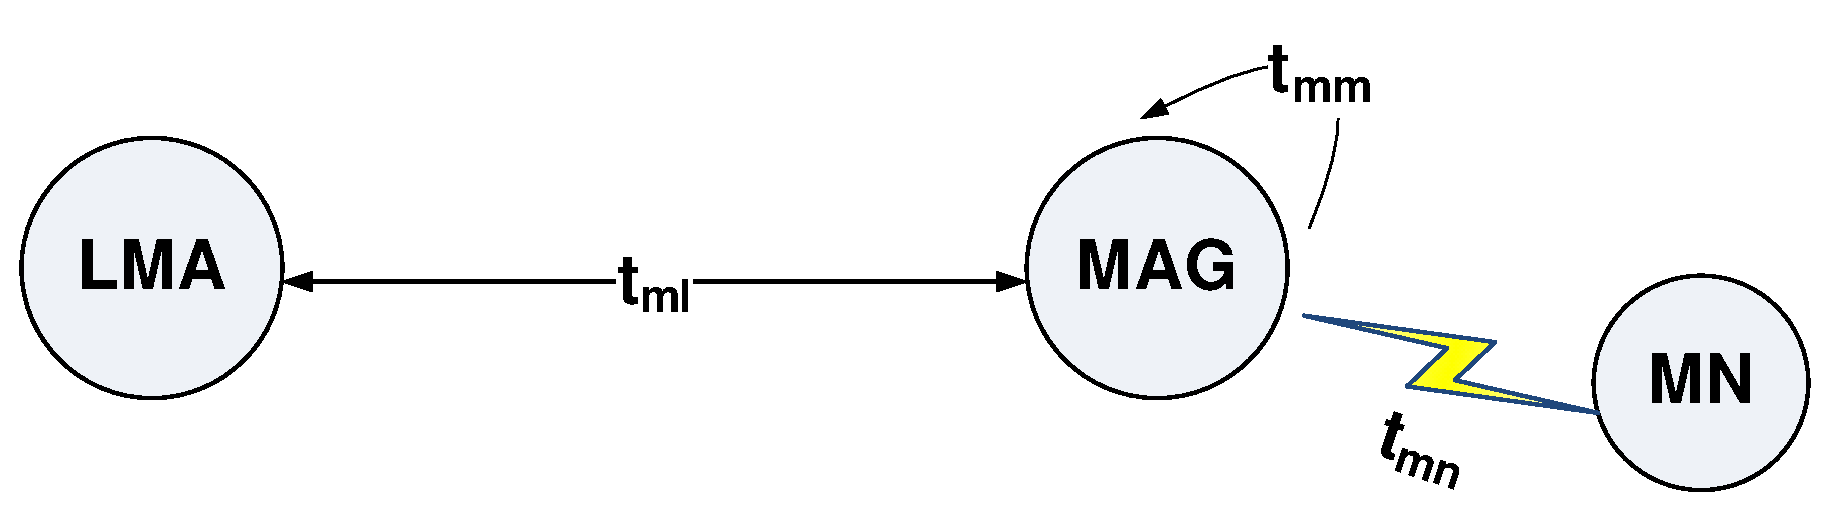
\includegraphics[width=0.50\textwidth]{./Part2/Chapter4/figures/c6_topology_analysis.eps} 
    \caption[Reference network topology for the  multicast service disruption time analysis.]{Reference network topology.}
     \label{fig:c6_topology_analysis}
  \end{center} 
\end{figure}

Fig.~\ref{fig:c6_topology_analysis} shows a reference topology for performance analysis. The delay factors consisting of total
delay are defined as follows:
\setlength \abovedisplayskip{-1pt}
\vspace{-0.1in}
\begin{itemize}
\itemsep 0.07em
\item $t_{mm}$: the delay between two MAGs.
\item $t_{ml}$: the delay between MAG and LMA.
\item $t_{mn}$: the delay between MAG and MN.
\item $t_{msa}$: the multicast service activation time.
\item $t_{qrd}$ the query response delay.
\end{itemize}

The service disruption time for multicast service is defined as a period when a multicast listener cannot receive the multicast packets. Thus, as can be seen in Fig.~\ref{fig:c6_handover}, it can be split into three main contributions (as stated in Chapter \ref{ch:performance_evaluation}): i) Layer 2 (L2) handover latency ($t_{L2}$); ii) Layer 3 (L3) handover duration ($t_{L3}$) caused by IP-related procedures. In PMIPv6, it includes the time for mobility management procedures (movement detection and location update procedures); and iii) The delay due to the multicast-related procedures, called $t_{M}(.)$.

Since in the proactive mode of M-LMA approach, it is not always feasible to the MN de-registers on the LMA by the previous MAG before attaching to the new one. Also, in the M-FPMIP approach, the under link radio access technology needs to support layer-2 triggers. Thus, in this section, the performance analysis will be done considering only the M-LMA (reactive-mode), the M-MLD and the M-CXT approaches. 

\begin{figure}[h!] 
 \begin{center} 
 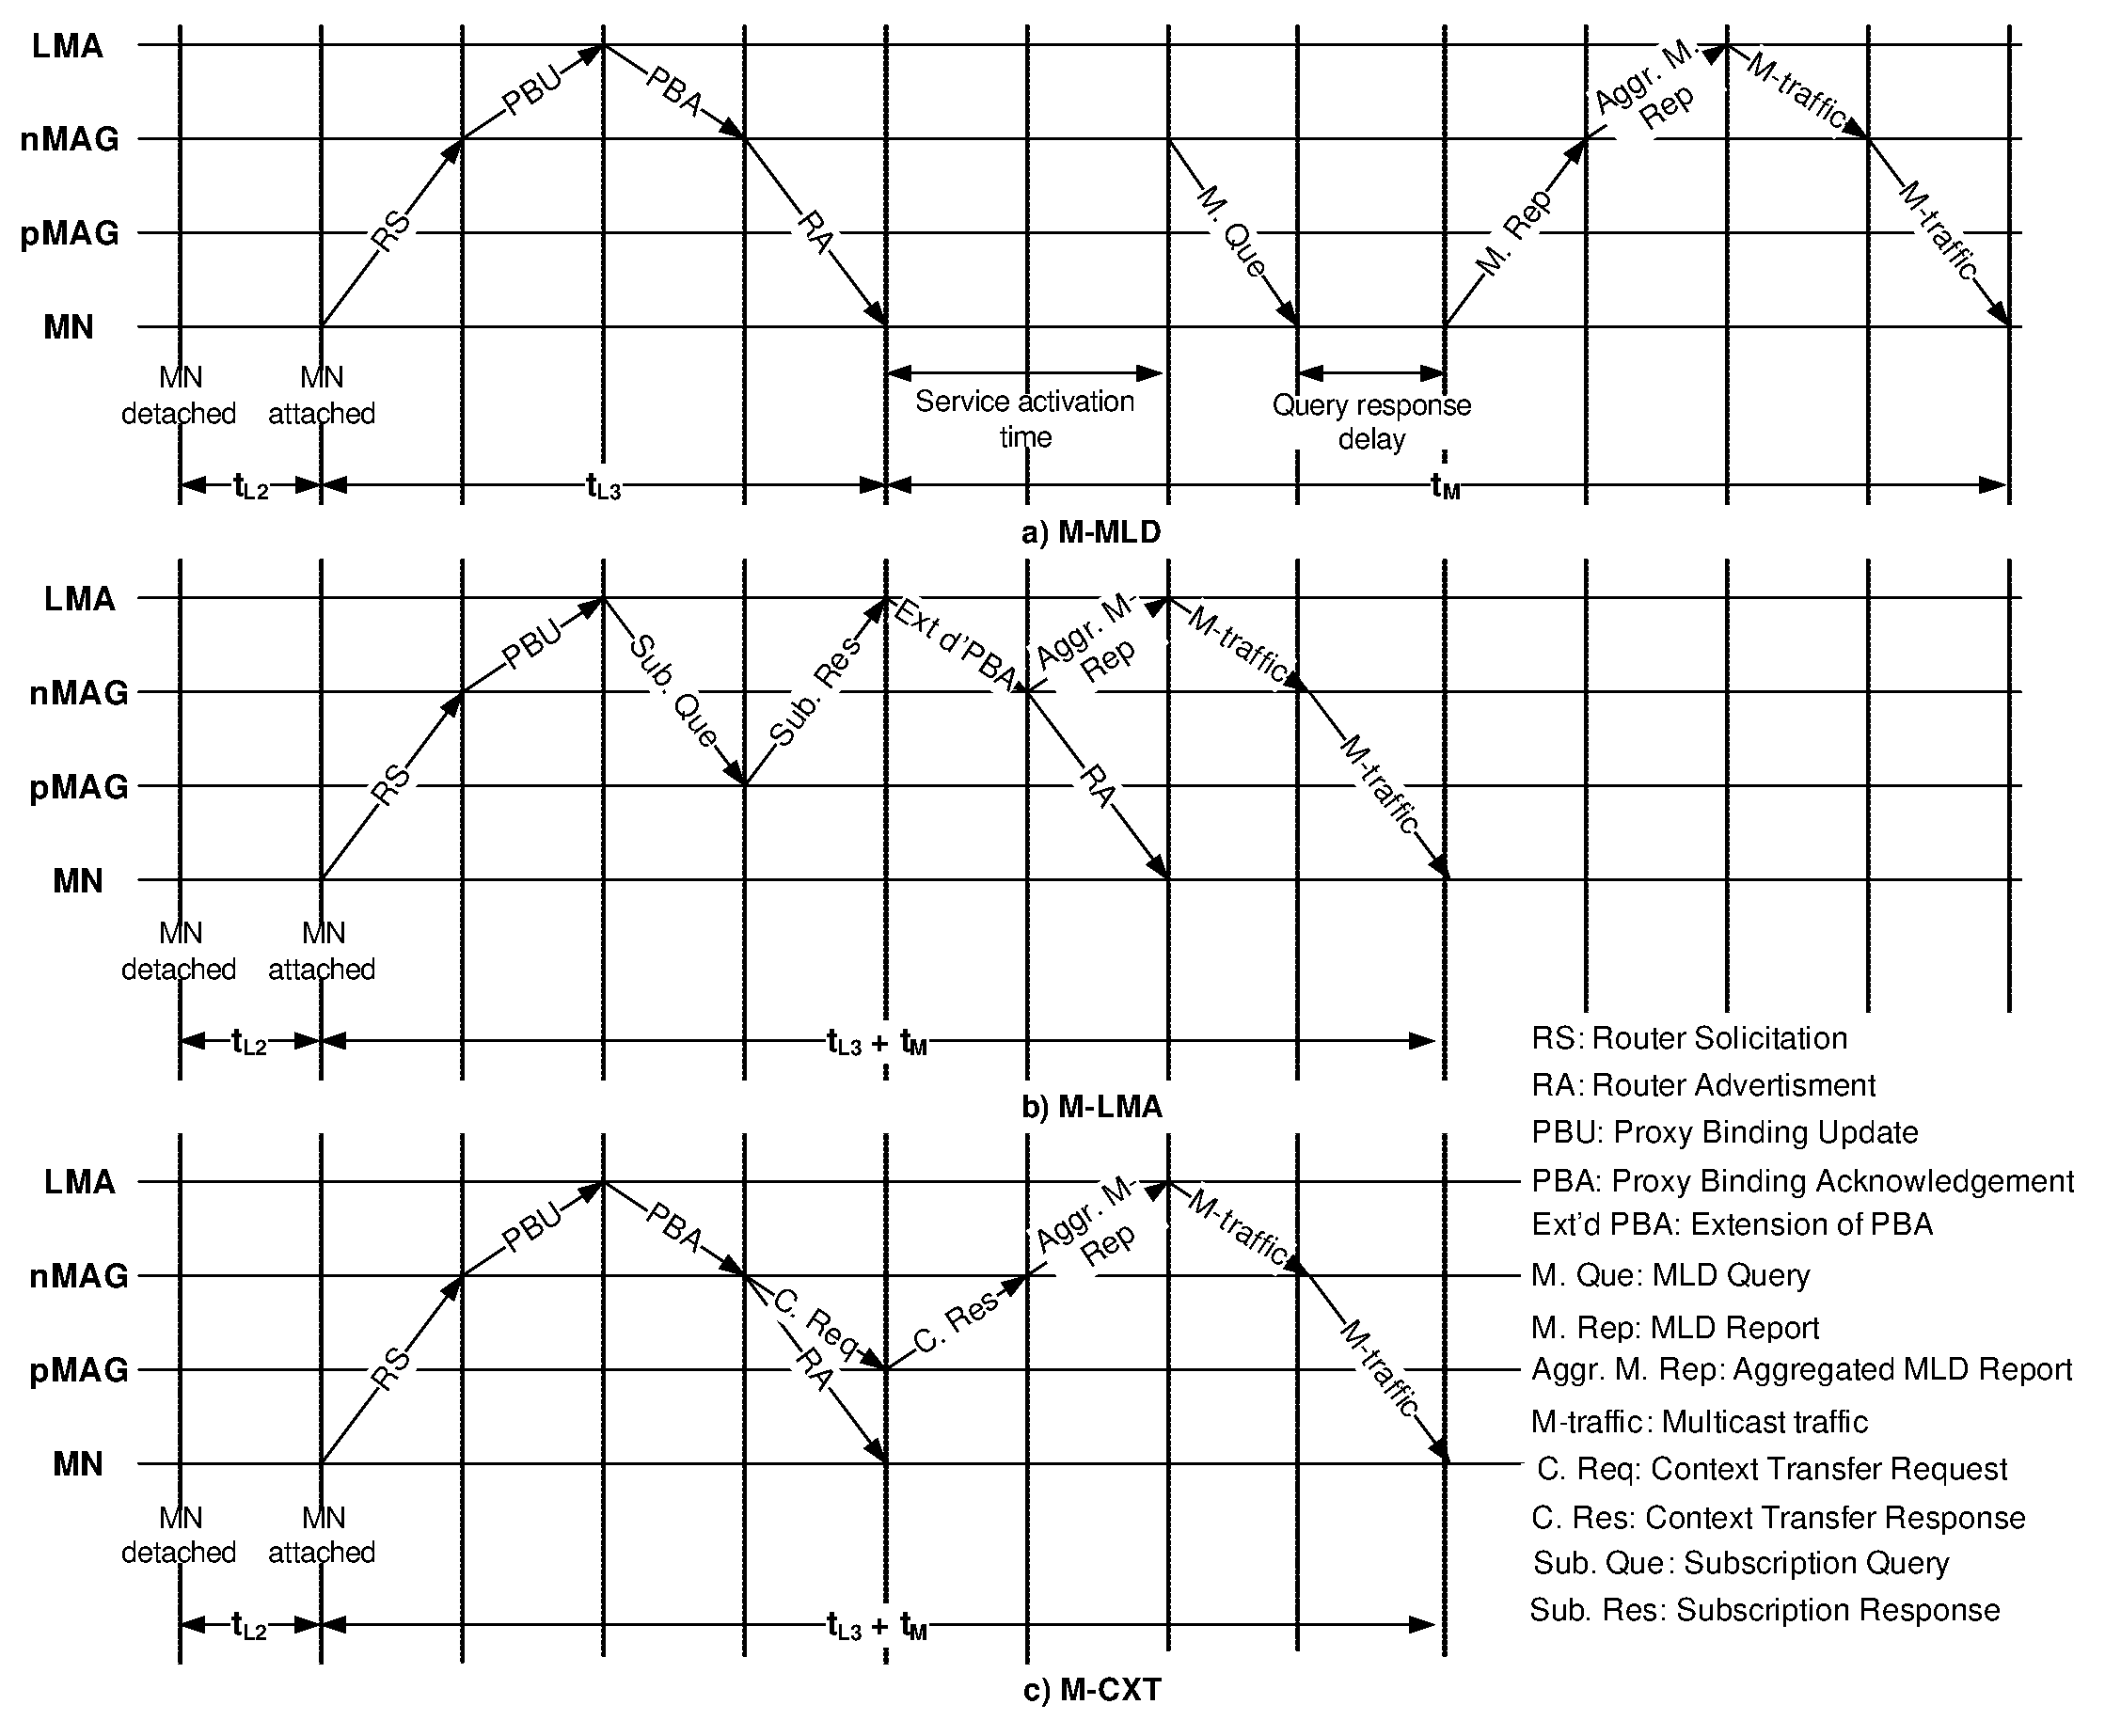
\includegraphics[width=0.85\textwidth]{./Part2/Chapter4/figures/c6_handover.eps} 
    \caption[Multicast-related signaling when a listener performs a handover inside a PMIPv6 domain.]{Multicast-related signaling for handover: (a) M-MLD, (b) M-LMA, (c) M-CXT.}
     \label{fig:c6_handover}
  \end{center} 
\end{figure}

Let $t_{X, Y}$ denote the delay between node X and node Y.  Then, the service disruption time is defined as \\
\begin{equation}
SD (.) = t_{L2} + t_{L3} + t_{M}(.),
\end{equation}
where $t_{L3}$ and $t_{M}(.)$ are given by\\
\begin{equation}
t_{L3} = 2t_{mn} + 2t_{ml}, 
\end{equation}
\begin{equation}
t_{M}(M-MLD) = t_{msa} + t_{qrd} + 3t_{mn} + 2t_{ml},
\end{equation}
\begin{equation}
t_{M}(M-LMA) = t_{mn} + 4t_{ml},
\end{equation}
\begin{equation}
t_{M}(M-CXT) = t_{mn} + 2t_{mm} +2t_{ml}.
\end{equation}

We suppose that MLD Queries are followed immediately the link-up event or the auto-configuration of IPv6 link-local address of an MN \cite{RFC_6224}. As a consequence, the multicast service activation time can be ignored ($t_{msa}$ = 0). As such, the total disruption time in the M-MLD approach is \\
\begin{equation}
SD(M-MLD) = t_{L2} + t_{qrd} + 5t_{mn} + 4t_{ml}.	
\label{eq:c6_total}
\end{equation}

In case of M-LMA approach, the service disruption is calculated as\\
\begin{equation}
SD(M-LMA) = t_{L2} + 2t_{mn} + 6t_{ml}. 	
\end{equation}

Using the multicast context transfer and the explicit tracking function, the context transfer function and layer 3 operations are executed in parallel as illustrated in Fig.~\ref{fig:c6_handover} (c). Consequently, the service disruption time in the M-CXT approach is calculated as follows\\
\begin{equation}
SD(M-CXT) = t_{L2} + 2t_{mn} + 2t_{mm} + 4t_{ml}. 	
\end{equation}

\section{Experimentation Setup and Scenarios Description} \label{section:testbed}
\begin{figure}[h!] 
 \begin{center} 
 \includegraphics[width=0.60\textwidth]{./Part2/Chapter4/figures/c6_testbed.eps} 
    \caption[PMIPv6 testbed for mobile multicast experimentation.]{Virtual PMIPv6 testbed.}
     \label{fig:c6_testbed}
  \end{center} 
\end{figure}

A reference topology for multicast support in a PMIPv6 domain is illustrated in Fig.~\ref{fig:c6_testbed}. The testbed - which consists of one LMA, three MAGs and two MNs, was developed based on the method described in Chapter \ref{ch:performance_evaluation}. For a quick reminder of this method, the testbed is a combination of virtual machines and wireless environment provided by the network simulator NS-3. The PMIPv6 entities (LMA, MAG) are the virtual machines while the access points (AP) and mobile nodes (MN0 and MN1) are NS-3 nodes. MN0 plays the role of a multicast source while MN1 plays the role of a multicast listener. Acting as a multicast listener, MN1 is subscribed to the multicast channel which is being broadcasted by the source. To deploy a PMIPv6 domain, the open source PMIPv6 implementation, named OAI PMIP \cite{oai_pmip}, is used. In OAI PMIPv6 implementation, the attachment/detachment phase for the MNs relies on SYSLOG \cite{syslog} message exchanged between Client (at the AP) and Server SYSLOG (at the MAG). Thus, the Client SYSLOG function is implemented in NS-3 and deployed at the APs. 

To enable the multicast support in a PMIPv6 domain, the MLD proxy function needs to be deployed at the MAG while the multicast routing function is provided at the LMA. There are two typical implementations of MLD proxy such as McProxy\footnote{McProxy - Multicast Proxy for IGMP/MLD, Homepage: http://mcproxy.realmv6.org/}, ECMH\footnote{ECMH - Easy Cast du Multi Hub, Homepage: http://unfix.org/projects/ecmh/}. Though the former is newer, it only supports MLDv1. That is why ECMH is selected. Yet, some functions need to be added into ECMH to support the multicast source mobility. On the other hand, the considered multicast routing protocols are PIM-SM/SSM \cite{PIM_SM}. There are two potential candidates providing PIM router functions: MRD6\footnote{MRD6, Homepage: http://fivebits.net/proj/mrd6/} and XORP\footnote{Xorp, Homepage: http://www.xorp.org/}. The first one is chosen because of its simplicity of deployment and configuration under UML. We also implemented the listener part of MLDv2 protocol under NS-3 to enable the multicast capability of NS-3 nodes.

\begin{figure}[h!] 
 \begin{center} 
 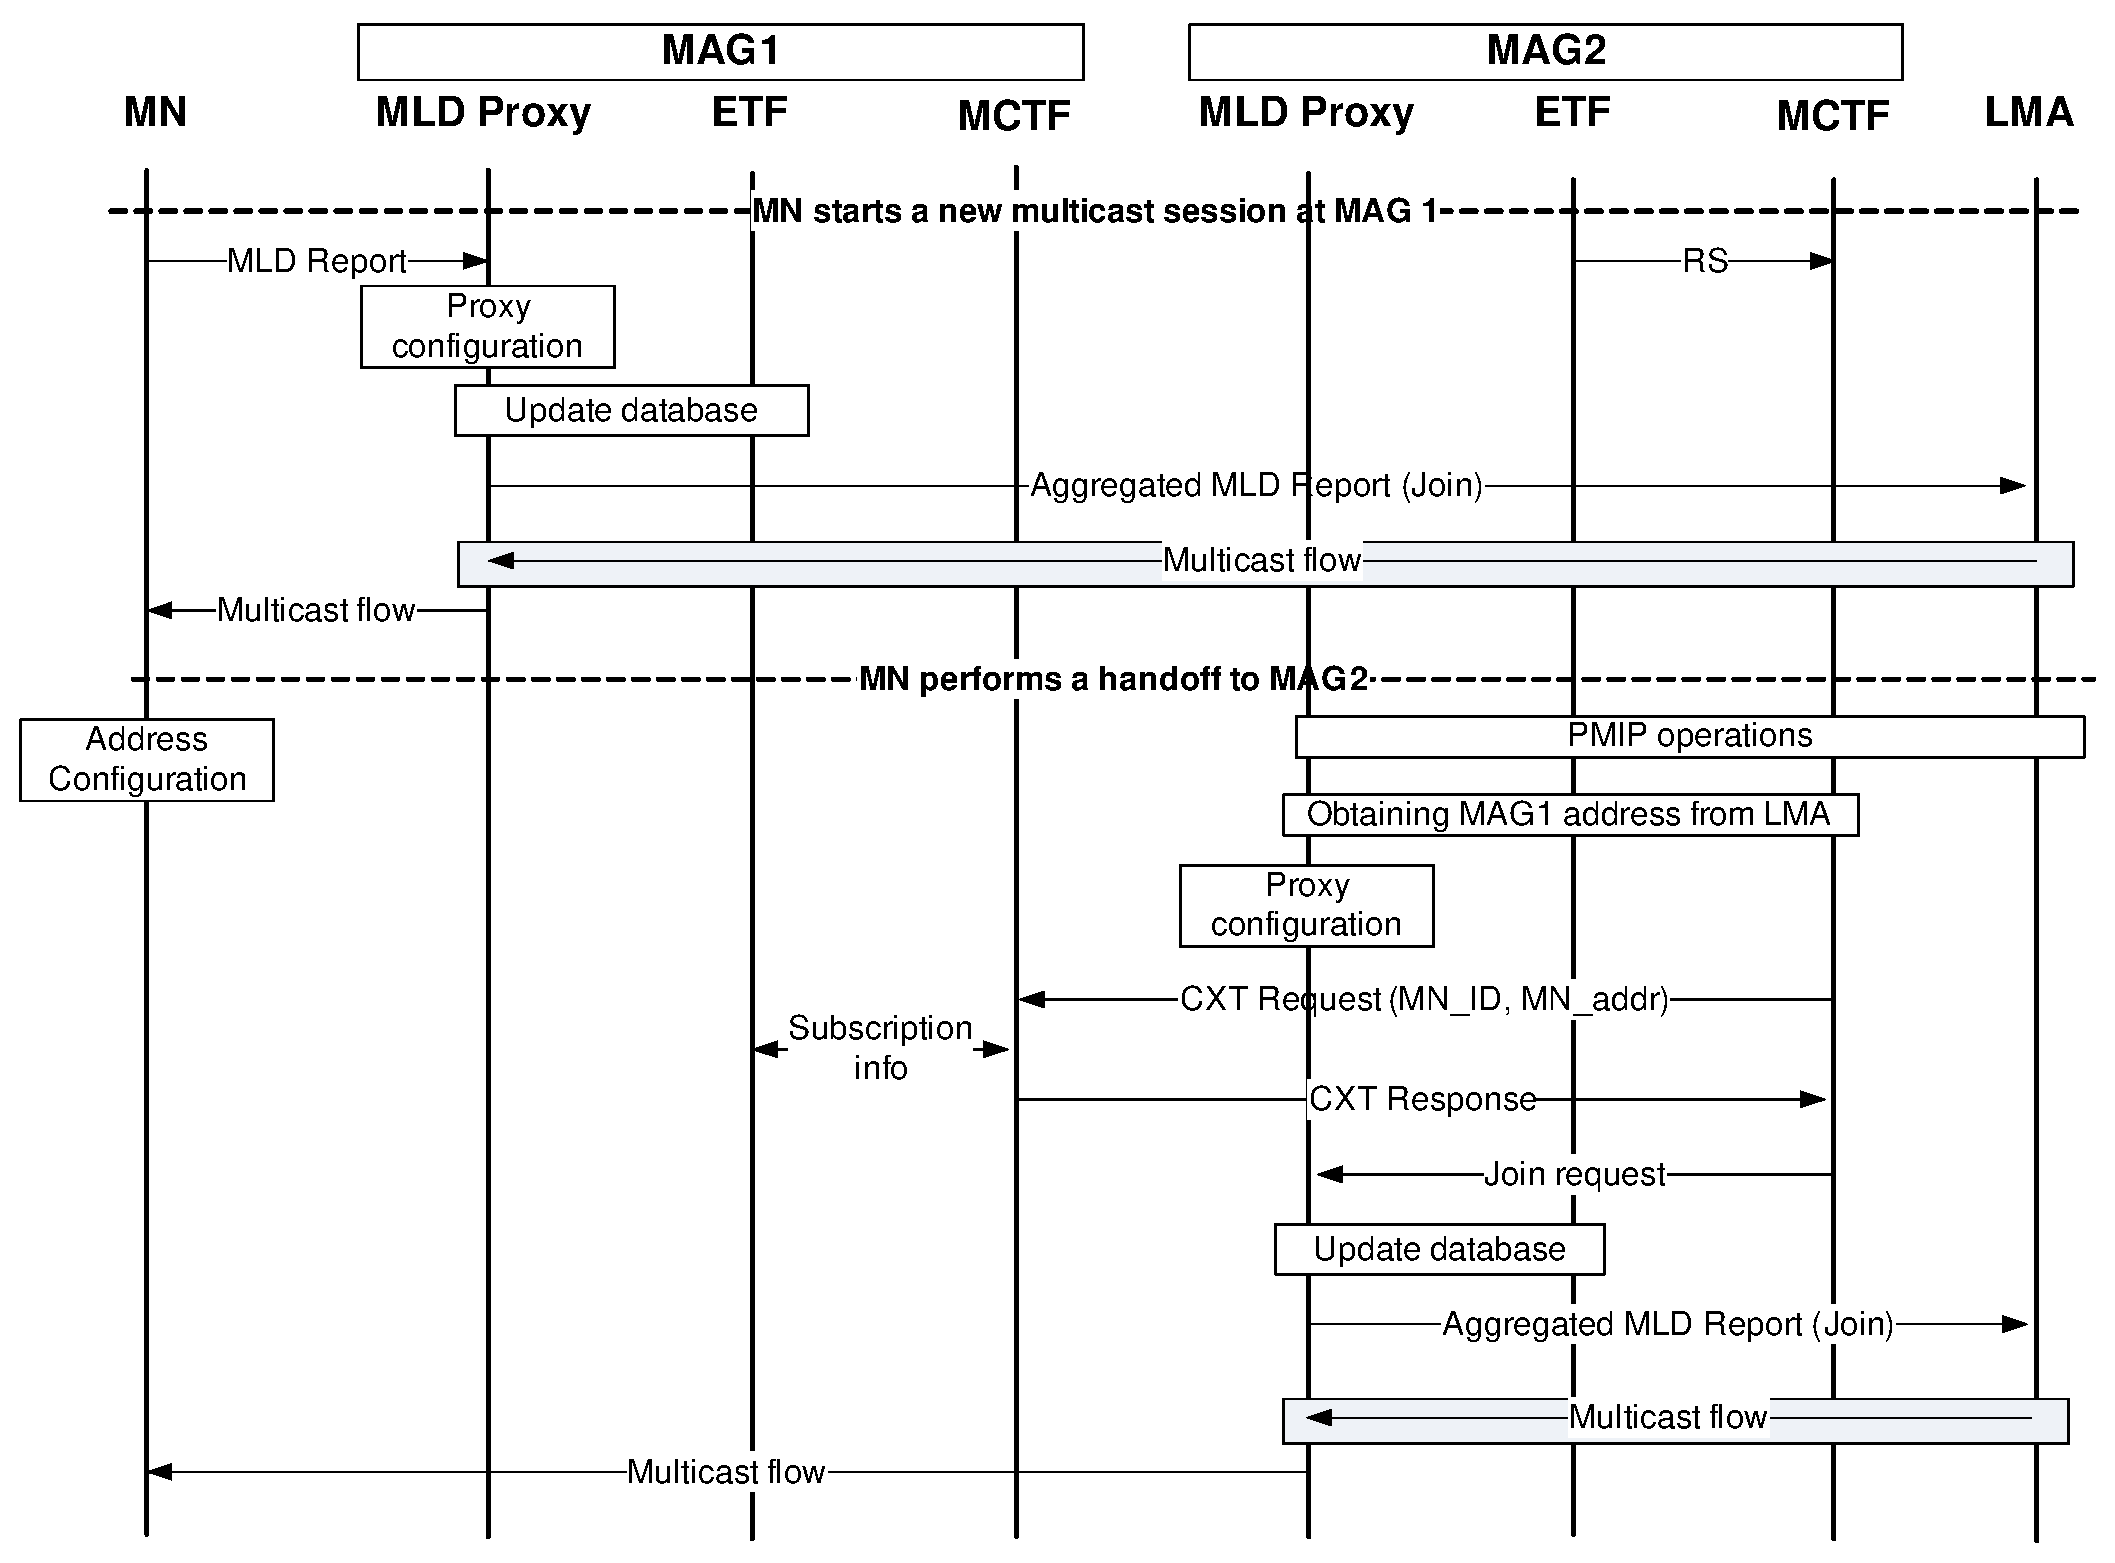
\includegraphics[width=0.750\textwidth]{./Part2/Chapter4/figures/c6_multicast_signaling.eps} 
    \caption[The interactions between components of the multicast mobility management module.]{Interaction between components of MUMO.}
     \label{fig:c6_multicast_signaling}
  \end{center} 
\end{figure}

In general, we implemented a multicast mobility management module (MUMO, in C/C++), which takes responsibility for all actions related to the multicast mobility as described in \cite{d4.2,d4.3} at the MAG. The structure of this module is briefly described as follows: i) The proxy function performs the operation of the MLD proxy (based on ECMH); ii) The explicit tracking function (ETF) maintains the per-host multicast membership state (can be considered as an extension to MLD proxy); and iii) The multicast context transfer function (MCTF) is responsible for the multicast context transfer exchanging between MAGs to reduce the service disruption time. The interaction between the different components of this module is illustrated in Fig.~\ref{fig:c6_multicast_signaling}. Note that the multicast context transfer function, which is developed as a separate sub-module, can be easily applied to the other solutions in PMIPv6 (e.g., direct-routing approach) as well as for the solutions in a DMM environment (see Chapter \ref{ch:multicast_dmm} for more details). 

From the fact that the service disruption time in M-CXT would be the same as in the M-LMA approach (as can be seen in Fig.~\ref{fig:c6_handover}), for a sake of simplicity we do not consider the M-LMA approach in our measurements. In other words, the experimentation will be conducted regarding only the M-MLD and the M-CXT approaches corresponding to two simulation scenarios as follows:
\begin{itemize}
\item Scenario 1: tuning the behavior of the MLD for routers (corresponding to the M-MLD approach). In this scenario, the regular behavior of MLD protocol takes place while the QRI is varied to measure the service disruption time. Upon receiving an MLD Query at the new link, the listener (MN1) replies by a regular MLD Report. Then, the nMAG sends an aggregated MLD Report to the LMA to join the multicast group on behalf of the listener. Thus, the multicast traffic originated from the source is routed from LMA to listener via the new tunnel LMA-nMAG. 
\item Scenario 2: using the multicast context transfer (corresponding to the M-CXT approach). When the multicast context transfer is used, by detecting the presence of a new listener, the multicast context transfer between nMAG and pMAG is executed, allowing nMAG to get the listener’s active multicast subscriptions. As an MLD proxy, nMAG joins the multicast group on behalf of the listener, and forwards the multicast packets to the listener.
\end{itemize}

To make sure that the experimental results reflect exactly the impact of the two strategies, the parameter QRI will be varied in both scenarios. According to \cite{MLDv2, tuning_MLD}, possible values of QRI using in the experimentation are 10, 5 and 2 seconds. Additionally, by now to simplify the experimentation, a simple mobility model is used: the listener moves between two MAGs with a fixed speed and a fixed direction. However, in the future, the mobility pattern will be applied to provide more flexible mobility of multicast listener. Also, the scenario in which many listeners are moving at the same time will be considered. To improve the credibility of the simulation results, we performed the experiment a large amount of times for each scenario. Based on the collected results, we calculate the average value and the standard deviation to improve the degree of confidence.

\section{Results and Discussions} \label{section:results}
\subsection{Results}
\paragraph{Numerical Results} In our analysis, $t_{L2}$, $t_{ml}$, $t_{mm}$ and $t_{mn}$ are assumed to be 50ms, 20ms, 10ms and 15ms, respectively, according to the literature \cite{d4.4}. Fig.~\ref{fig:c6_numerical_result} shows the numerical results. It is observed that the service disruption time in the M-MLD approach is definitely higher than that in the other approaches. On the other hand, the service disruption in case of M-CXT is a bit smaller than that in M-LMA (smaller is better). In other words, the M-CXT approach in general gives a similar performance in terms of service disruption as the M-LMA approach.
\begin{figure}[h!] 
 \begin{center} 
 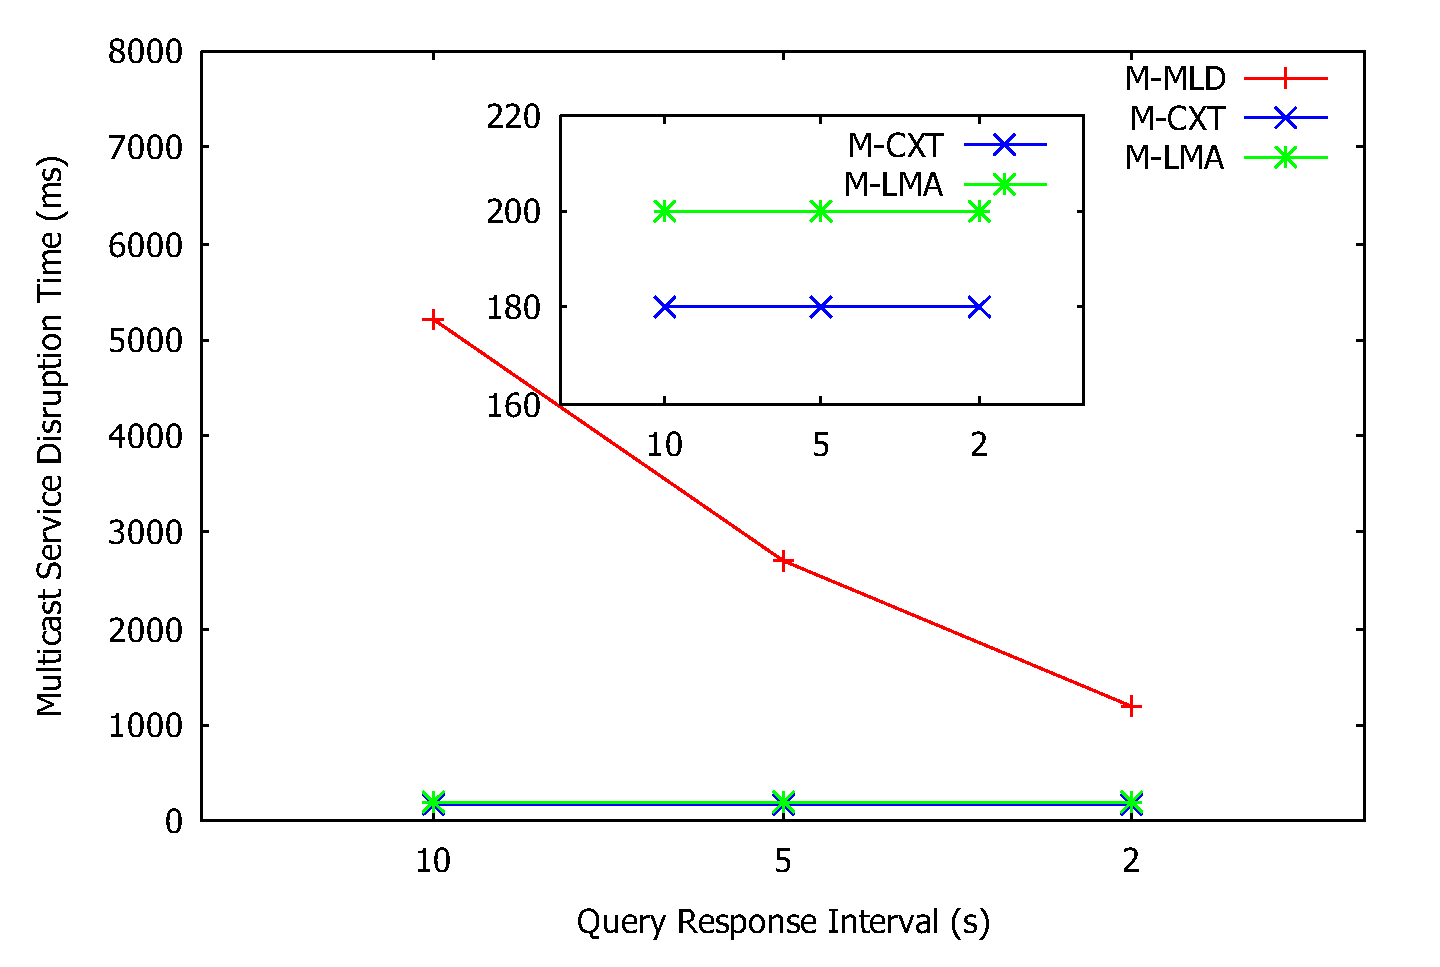
\includegraphics[width=0.60\textwidth]{./Part2/Chapter4/figures/c6_numerical_result.eps} 
    \caption[The multicast service disruption time: numerical results.]{Service disruption time: numerical results.}
     \label{fig:c6_numerical_result}
  \end{center} 
\end{figure}
\paragraph{Experimental Results} Fig.~\ref{fig:c6_simulation_result} describes the experimental results for the service disruption time in terms of mean ($<x>$) and standard deviation ($<\sigma_{x}>$). It appears clearly that the service disruption time in the M-MLD approach is absolutely higher than that in the M-CXT due to the value of $t_{qrd}$. As expected, the service disruption time in the former case decreases proportionally with the QRI, while almost keeping as a constant as the decreasing of QRI in the latter case. 
\begin{figure}[h!] 
 \begin{center} 
 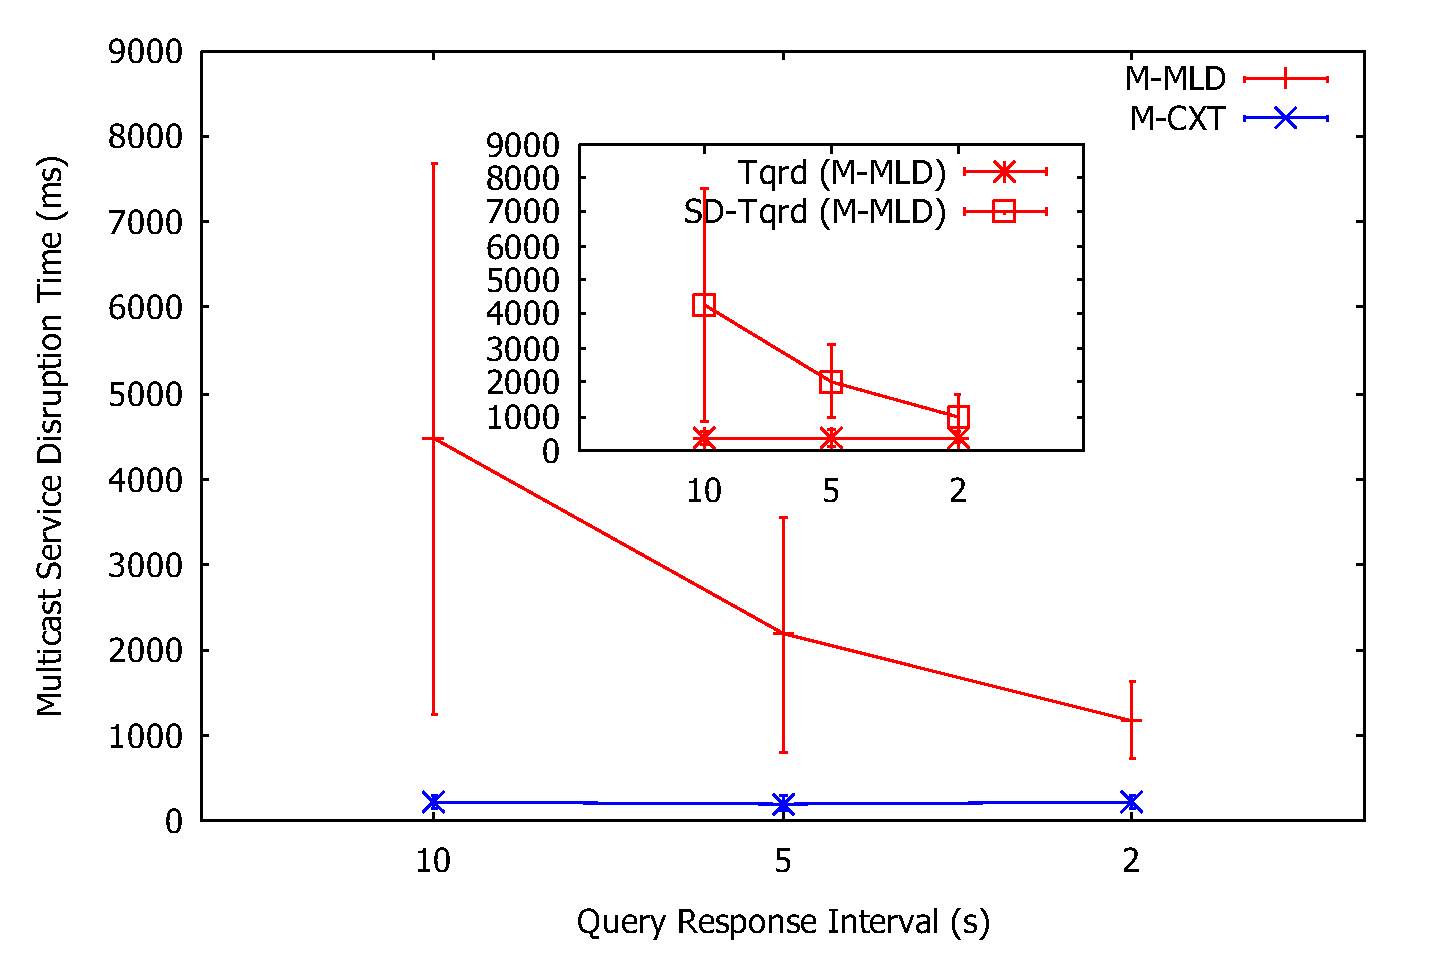
\includegraphics[width=0.60\textwidth]{./Part2/Chapter4/figures/c6_simulation_result.eps} 
    \caption[The multicast service disruption time: experimental results.]{Service disruption time: experimental results.}
     \label{fig:c6_simulation_result}
  \end{center} 
\end{figure}
The average value of service disruption time in the M-MLD is 1180ms ($\sigma$= 445.4ms) in the best case (when QRI is set to 2s), which still makes the impact of handover noticeable. If the multicast context transfer is used (M-CXT), in average, the service disruption time is around 220.53ms. Consequently, the handover impact on the quality of multicast stream is almost imperceptible. The variation of service disruption time in the M-MLD approach is clearly seen since it depends on several factors like scanning, association, authentication and $t_{qrd}$. Even $t_{qrd}$ can spread out over the large interval [0, QRI], $<t_{qrd}>$ is definitely higher than that of other delay types (L2 and L3). Hence, $t_{qrd}$ is the crucial factor in the service disruption time.
\begin{figure}[h!] 
 \begin{center} 
 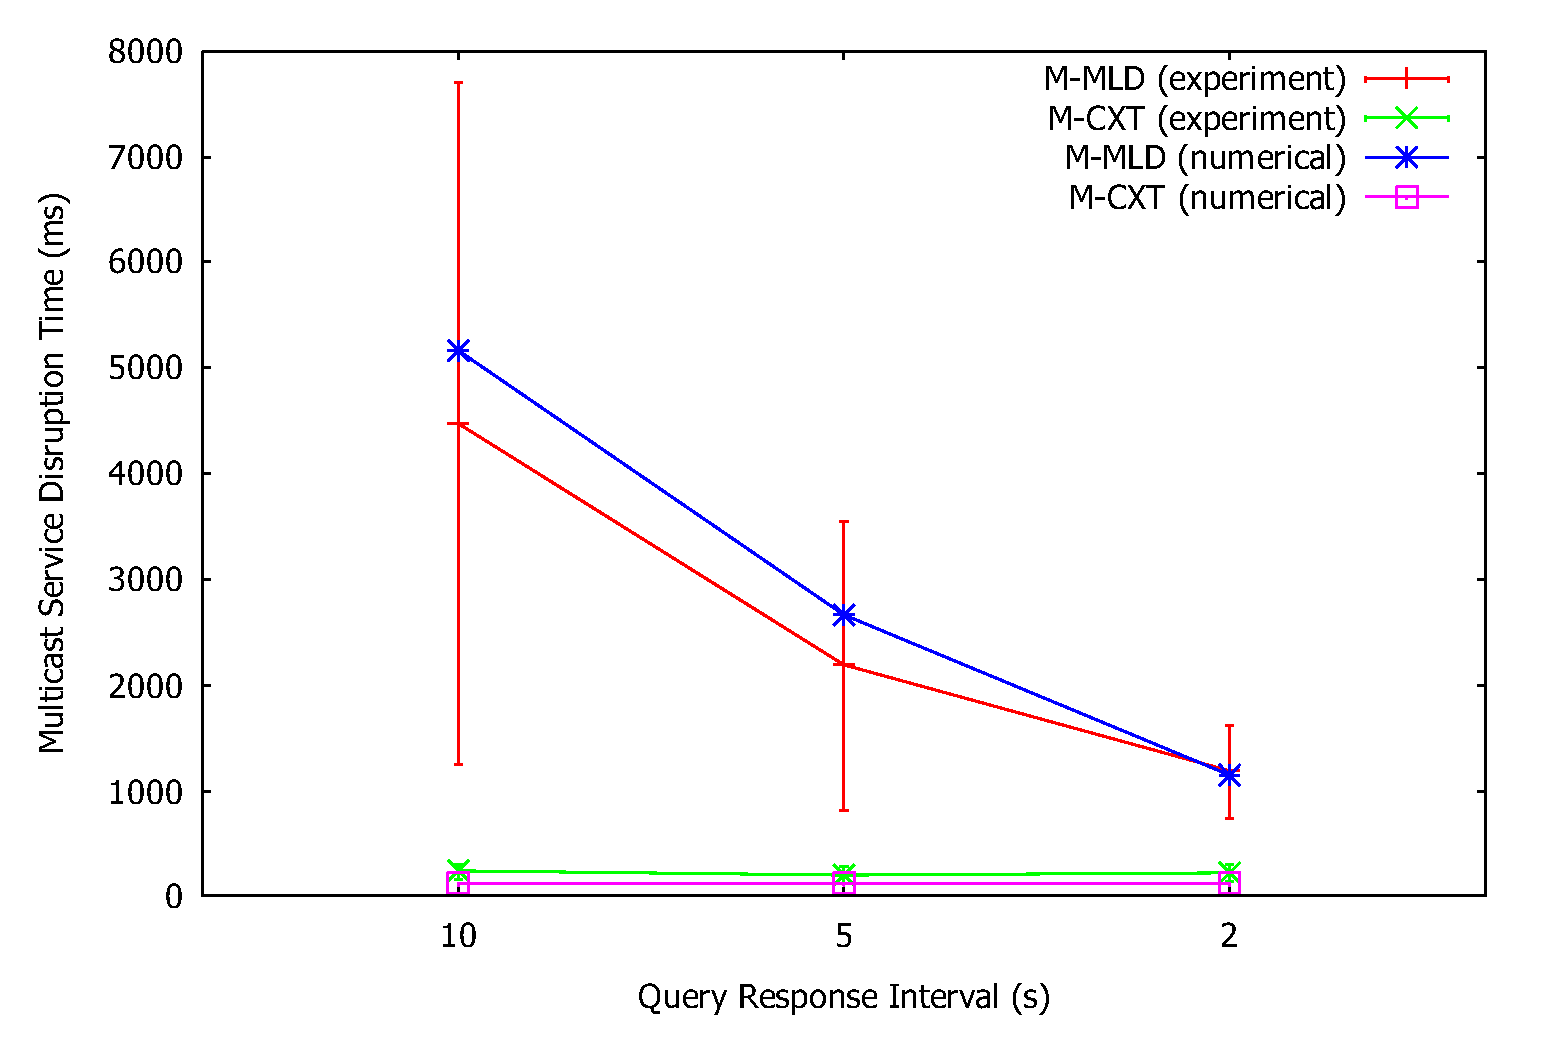
\includegraphics[width=0.60\textwidth]{./Part2/Chapter4/figures/c6_comparision.eps} 
    \caption[The multicast service disruption time: experimental vs. numerical results.]{Service disruption time: experimental vs. numerical results.}
     \label{fig:c6_comparision}
  \end{center} 
\end{figure}
\paragraph{Numerical vs. Experimental Results} Now the comparison between the numerical and the experimental results is investigated. For a fair comparison, we do not consider $t_{L2}$, since it depends on a specific wireless technology. Fig.~\ref{fig:c6_comparision} describes the numerical and experimental results. It is observed that the experimental results are, in general, in line with the theoretical analysis.
\subsection{Discussions}
\paragraph{Impact of QRI Reduction on the Wireless Link Condition}
If no multicast context transfer is used, the service disruption during handover can be clearly seen, even in the best case (QRI=2s). To minimize the handover effect, the value of the query response delay ($t_{qrd}$) needs to be reduced. It is done by decreasing the QRI. This reduction facilitates to achieve a seamless handover but makes the traffic more bursty, leading to the signaling overhead over the air interface. 

Following the MLDv2 protocol operation, after receiving an MLD query (periodical query or a query caused by a link-up event), the multicast listeners reply by an MLD Report at the interval selected randomly from the range [0, QRI]. As such, during the period [0, QRI] there are $n$ MLD Report messages generated on the link (where $n$ is the number of multicast nodes attached to MAG). The number of signaling messages is dramatically increased compared with those in case of the context transfer (only 2 messages are exchanged between MAGs via a wired link). 
The total air interface signaling overhead in the uplink direction is calculated as the size of MLD Report message multiplied by the number of MLD Report messages per second. Let $s$ denote the average size of MLD Report message, which is 96 bytes \cite{d4.3}. Thus, the total overhead is expressed as\\
\begin{equation}
OH = \frac{n \cdot s}{QRI}
\end{equation}

From the experimental results, $SD(M-CXT)$ in the worst case is 507.5ms. From Eq. (\ref{eq:c6_total}), to achieve a similar delay without any context transfer, $t_{qrd}$ must be less than or equal to a value of 352.4ms (when $t_{L2}$ = 0.1ms). It is done by setting QRI to a value of 352.4ms. It was also proven by the simulation results in which the mean and standard deviation of service disruption time are 465.43 and 70.3 ms, respectively. With this value of QRI, Fig.~\ref{fig:c6_mld} illustrates the air interface overhead. In more details, Fig. \ref{fig:c6_mld_n} shows the overhead as a function of the number of listeners attached to one MAG. As the number of listeners increases, the signaling overhead increases. For example, considering a typical PMIPv6 deployment in which a MAG severs approximately 5000 MNs \cite{RFC_6224}, the signaling overhead is 10896 kbits/s ($\approx 10.8 Mbit/s$). It may cause a negative impact to the wireless network since the wireless link is a typically bandwidth limited. 
Fig~.\ref{fig:c6_mld_qri} shows the signaling overhead when the value of QRI is varied over a range [100, 2000]ms. The overhead decreases when QRI increases. When QRI is small, the signaling overhead causes a noticeable impact to the wireless link. Thus, it is obvious that reducing the service disruption by using QRI should be carefully investigated at a cost of high signaling overhead and increase of power consumption at the mobile node. 

\begin{figure}[h!]
\centering
\subfloat[]{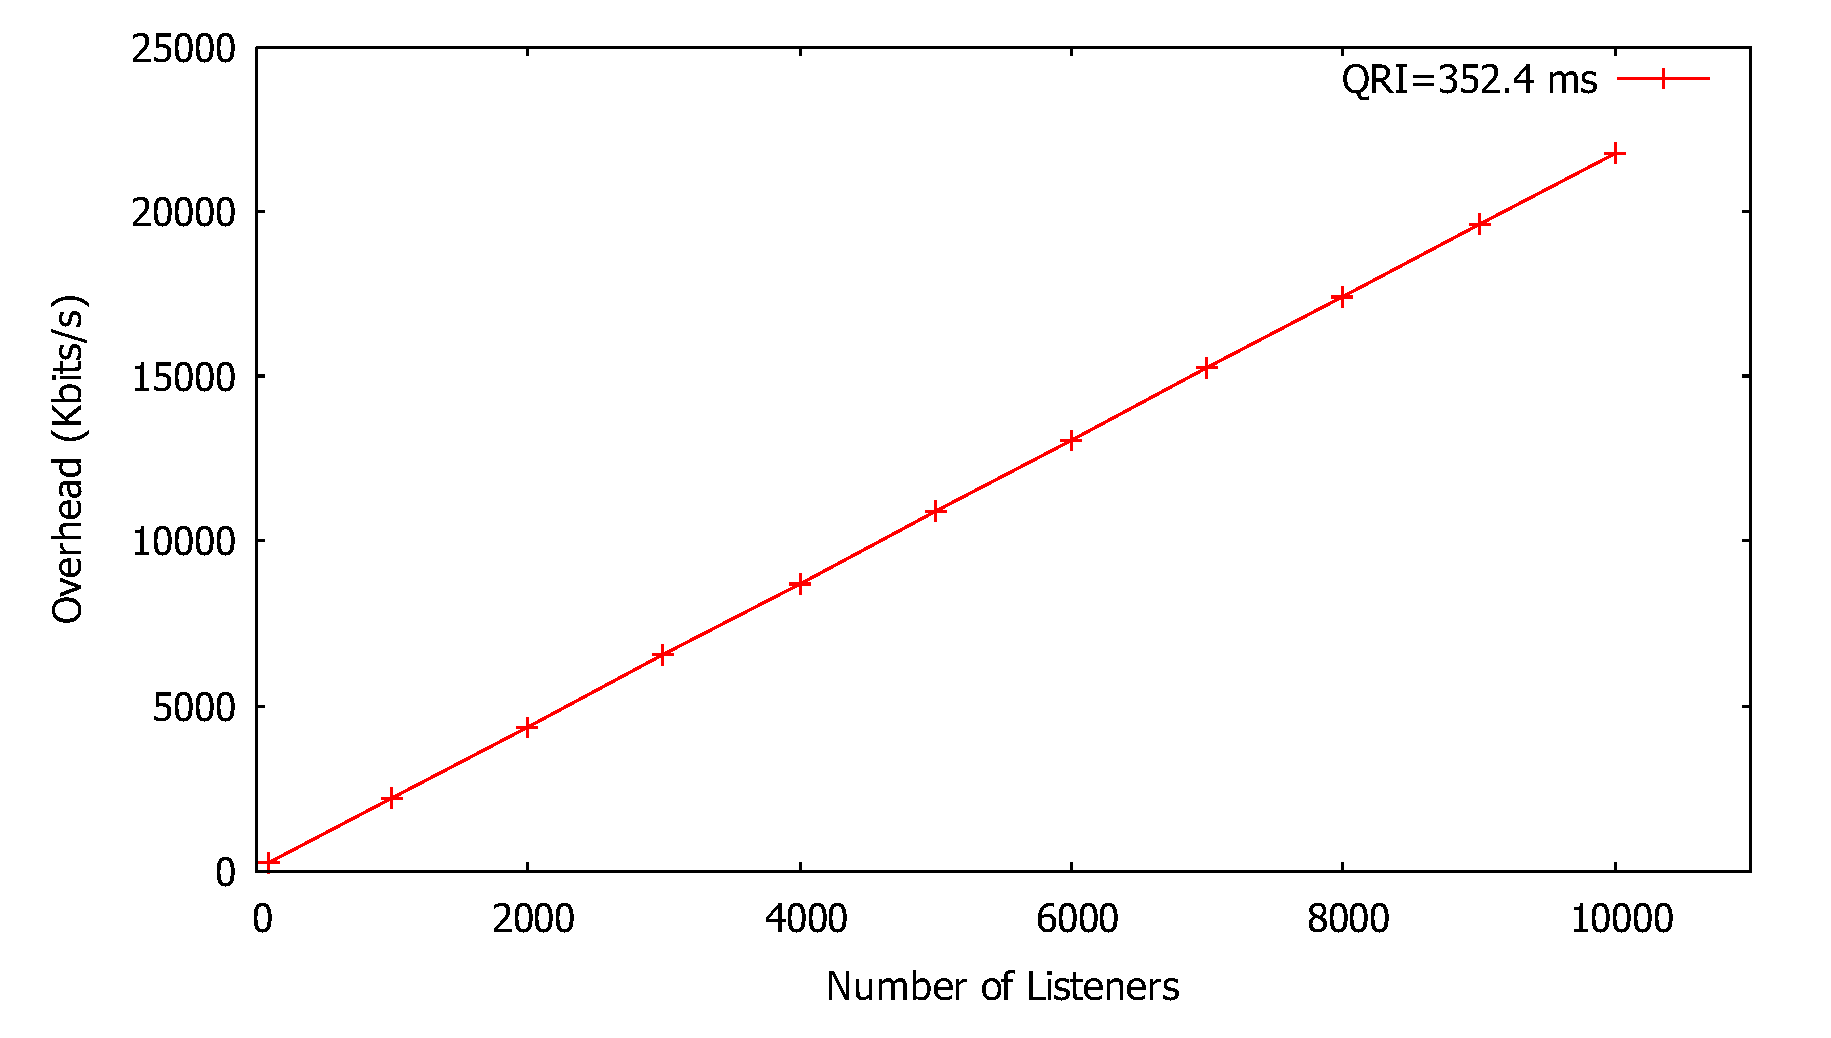
\includegraphics[width=0.47\textwidth]{./Part2/Chapter4/figures/c6_mld_n.eps} \label{fig:c6_mld_n}}\,\,\,\,\,\,
\subfloat[]{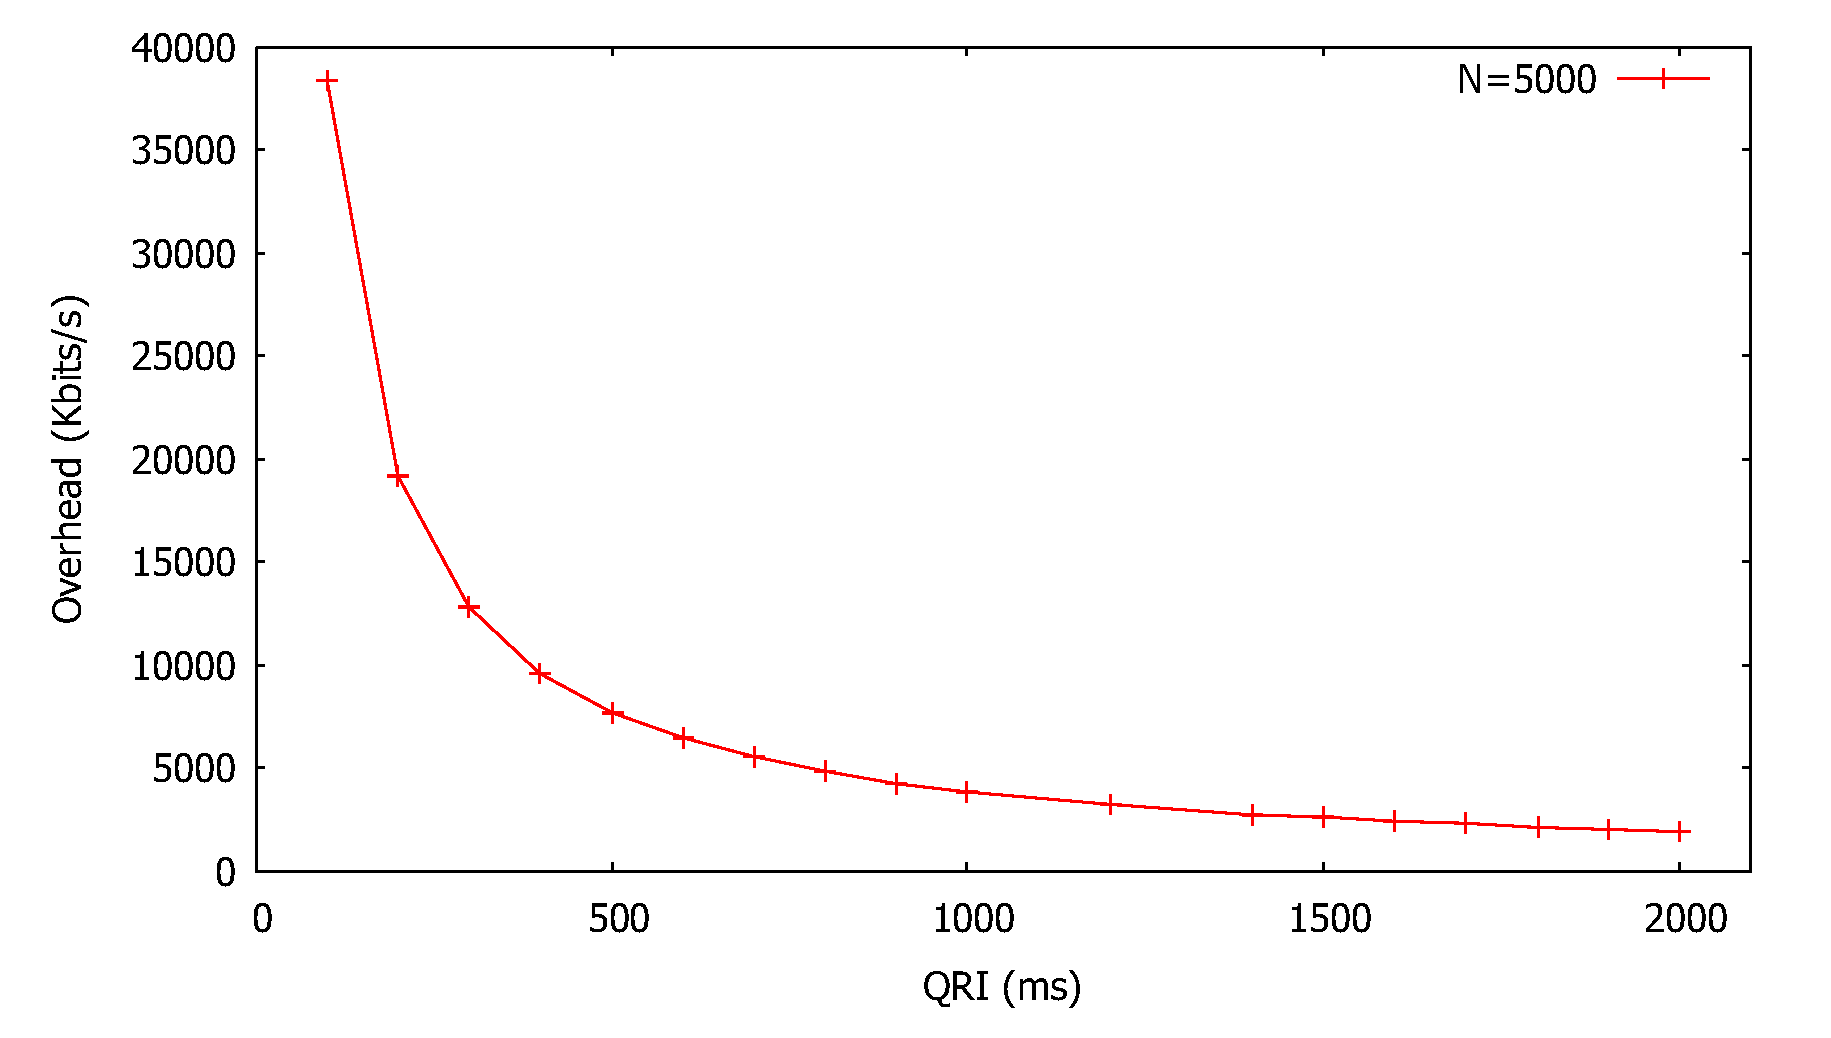
\includegraphics[width=0.47\textwidth]{./Part2/Chapter4/figures/c6_mld_qri.eps}\label{fig:c6_mld_qri}}
\caption[Multicast-related signaling overhead over the air interface.]{Air Interface signaling overhead: (a) as a function of number of listeners (n), (b) as a function of QRI.}
\label{fig:c6_mld}
\end{figure}

\paragraph{Waste of Resource (Leave Latency) Issue}
Due to mobility, the listener moves from the pMAG to the nMAG without explicitly sending an MLD message to leave the multicast group at the pMAG. As a result, if the listener is the last member of this group, the pMAG still continues forwarding this flow until it updates the membership information. In more details, according to \cite{MLDv2} the MLD proxy at pMAG has to wait to the source timer expires, then sends a source specific query and waits for a report during the time specified by the value of Last Listener Query Timer (LLQT) (during LLQT time, the pMAG should send Last Listener Query Count (LLQC) - 1 retransmissions of the query). The source timer at the beginning is set to the value of the Multicast Address Listening Interval (MALI). As a result, the total time needed for the pMAG to recognize that the last member has left its subnet is calculated as \\
\begin{equation}
LL = MALI - T_{leave} + LLQT,
\end{equation}
where 
\begin{equation}
MALI = RV \cdot QI + QRI,
\end{equation}
\begin{equation}
LLQT=  LLQI \cdot LLQC,
\end{equation}
where LLQI is Last Listener Query Interval and RV is the Robustness Variable. 
$T_{leave}$ is the interval time between the last source timer update and the moment where the listener leaves the pMAG. Thus, in average\\
\begin{equation}
T_{leave} = \dfrac{QI+QRI}{2}
\end{equation}

Without the explicit tracking function, the default value of RV, QRI, QI, LLQI and LLQC is 2, 10s, 125s, 1s and 2, respectively.  While in case of explicit tracking function, the value of RV can be set to 1 or 2 depending on the link condition \cite{tuning_MLD}. Also, QRI may be set to 5, 10, and 20s. Thus, in the normal case, the leave latency is 194.5s, while in case of explicit tracking is 191s (in the best case, where RV and QRI are set to 1s and 5s, respectively). During this period, the pMAG continues forwarding the multicast traffic even though no listener is interested in this flow, leading to a significant waste of resource. Even with the explicit tracking function, the leave latency is slightly reduced. Taking benefit of the context transfer function, the nMAG can request the pMAG to stop forwarding the multicast flow by means of CXT Request message (see Fig.~\ref{fig:c6_multicast_signaling}). Thanks to this mechanism, in our experiment the leave latency is 105.6ms (standard deviation = 45.2). Thus, the leave latency is negligible.   

\section{Conclusion} \label{section:conclusion}
This chapter focused on the effect of using the multicast context transfer and tuning the behavior of the IGMP/MLD for routers on handover performance of multicast listener mobility. The numerical and experimental results showed that through the utilization of multicast context transfer, the service disruption time could be reduced significantly without increasing the multicast-related signaling. We also observed that by tuning the behavior of the IGMP/MLD for routers, we could achieve a similar result, but make a noticeable multicast-related signaling increase. Thus, the impact of the multicast-related signaling on the wireless link by the number of listeners and the value of QRI was studied. In addition, the solution based on the multicast context transfer helps minimizing the handover latency. This chapter also presented an enhanced version of the testbed described in Chapter \ref{ch:performance_evaluation} by introducing the multicast mobility support. We deployed a real implementation for the multicast context transfer and explicit tracking functions on our testbed. This implementation then can be directly applied in a real testbed. In more details, in the Medieval project, the real multicast testbed \cite{d4.3, d4.4} has been deployed to validate the effective of multicast context transfer for PBS consumers over a DMM environment.   


\chapter{Load Balancing of Multicast Flows in PMIPv6 Networks} \label{ch:LB} 
\section{Introduction}
The increasing penetration of the mobile devices, such as tablets and smart phones is generating a huge number of data traffic, especially video traffic over mobile networks \cite{ericsson,cisco_forecast}. In this context, it is common to have a huge number of devices associated with the LMA in a PMIPv6 domain, thus, easily making the LMA a bottleneck and single point of failure. Consequently, the quality of the ongoing sessions could be degraded (e.g., longer queuing delay, and increased packet loss). In this context, mobile network operators may need to deploy multiple LMAs in a large PMIPv6 domain, so that the traffic can be distributed among the LMAs \cite{PMIPv6}. Yet, it is highly possible that some LMAs become overloaded while others are underutilized. Consequently, load balancing (LB) among the LMAs is needed.

From the fact that multicast is expected to be widely deployed in the near future to deal with a huge demand of multimedia traffic, as well as the mobile video content typically has much higher bit rates than the other content types, the multicast service should play a crucial factor in putting load on the LMA. However, its role has been neglected in all existing LB proposals. Therefore, the consideration of multicast in the existing LB mechanisms can lead to several issues from both LB (efficiency degradation) and multicast service perspective (e.g., tunnel convergence problem and service disruption). 

For these reasons, a LB mechanism which takes the multicast service into account is needed. In this chapter, we will introduce such LB mechanism, the so-called multicast-based mechanism. The key idea is that by separating the multicast LB from the unicast LB, the proposed solution helps better distribute the load among the LMAs in runtime, thus, improving the efficiency of resource utilization. In details, when an LMA is overloaded, a multicast session will be selected to move to a less loaded one. The LB will also be executed when a listener starts a new multicast session to select the appropriate LMA to serve this session. As a result, the proposed solution does not influence the ongoing unicast/multicast sessions (except the selected session with which the multicast service disruption, in most cases, satisfies the requirements for the real-time services \cite{interruption_requirements}). It is noted that this chapter mainly focuses on the multicast listener.  

The rest of this chapter is organized as follows. Section \ref{ch7:existing_solution} highlights the issues when considering multicast with the existing LB mechanisms. Section \ref{ch7:solution} introduces the multicast-based LB as well as the criteria for the LMA and multicast session selection. Section \ref{ch7:performance_analysis} presents the performance analysis regarding LMA load and multicast service disruption. Section \ref{c7:experiment} takes a look on the experiment testbed including the testbed description, the experiment scenarios and the collected results. Finally, Section \ref{ch7:conclusion} concludes this chapter.

\section{Multicast Consideration in the Existing LB Mechanisms}\label{ch7:existing_solution}
There are two main approaches for LB among LMAs in PMIPv6, namely, proactive-MN and reactive-MN. In the proactive-MN approach \cite{runtime_lma, lma_discovery}, the LB will be executed in the initial phase of an MN to select the least loaded LMA. This approach only takes the current load of the LMAs (neither unicast nor multicast service) into account. All mobility sessions of this MN then would be anchored at the assigned LMA during their lifetime in the domain. The main advantage of this approach is that it does not influence the ongoing sessions of the registered MNs. However, since it is executed in the initial phase of an MN, the varying session rate and data rate may cause the unfair load distribution among the LMAs. When an LMA is overloaded, it may drop the new sessions. It also causes several issues for the ongoing sessions such as service disruption and packet loss. 
\begin{figure}[h!] 
 \begin{center} 
 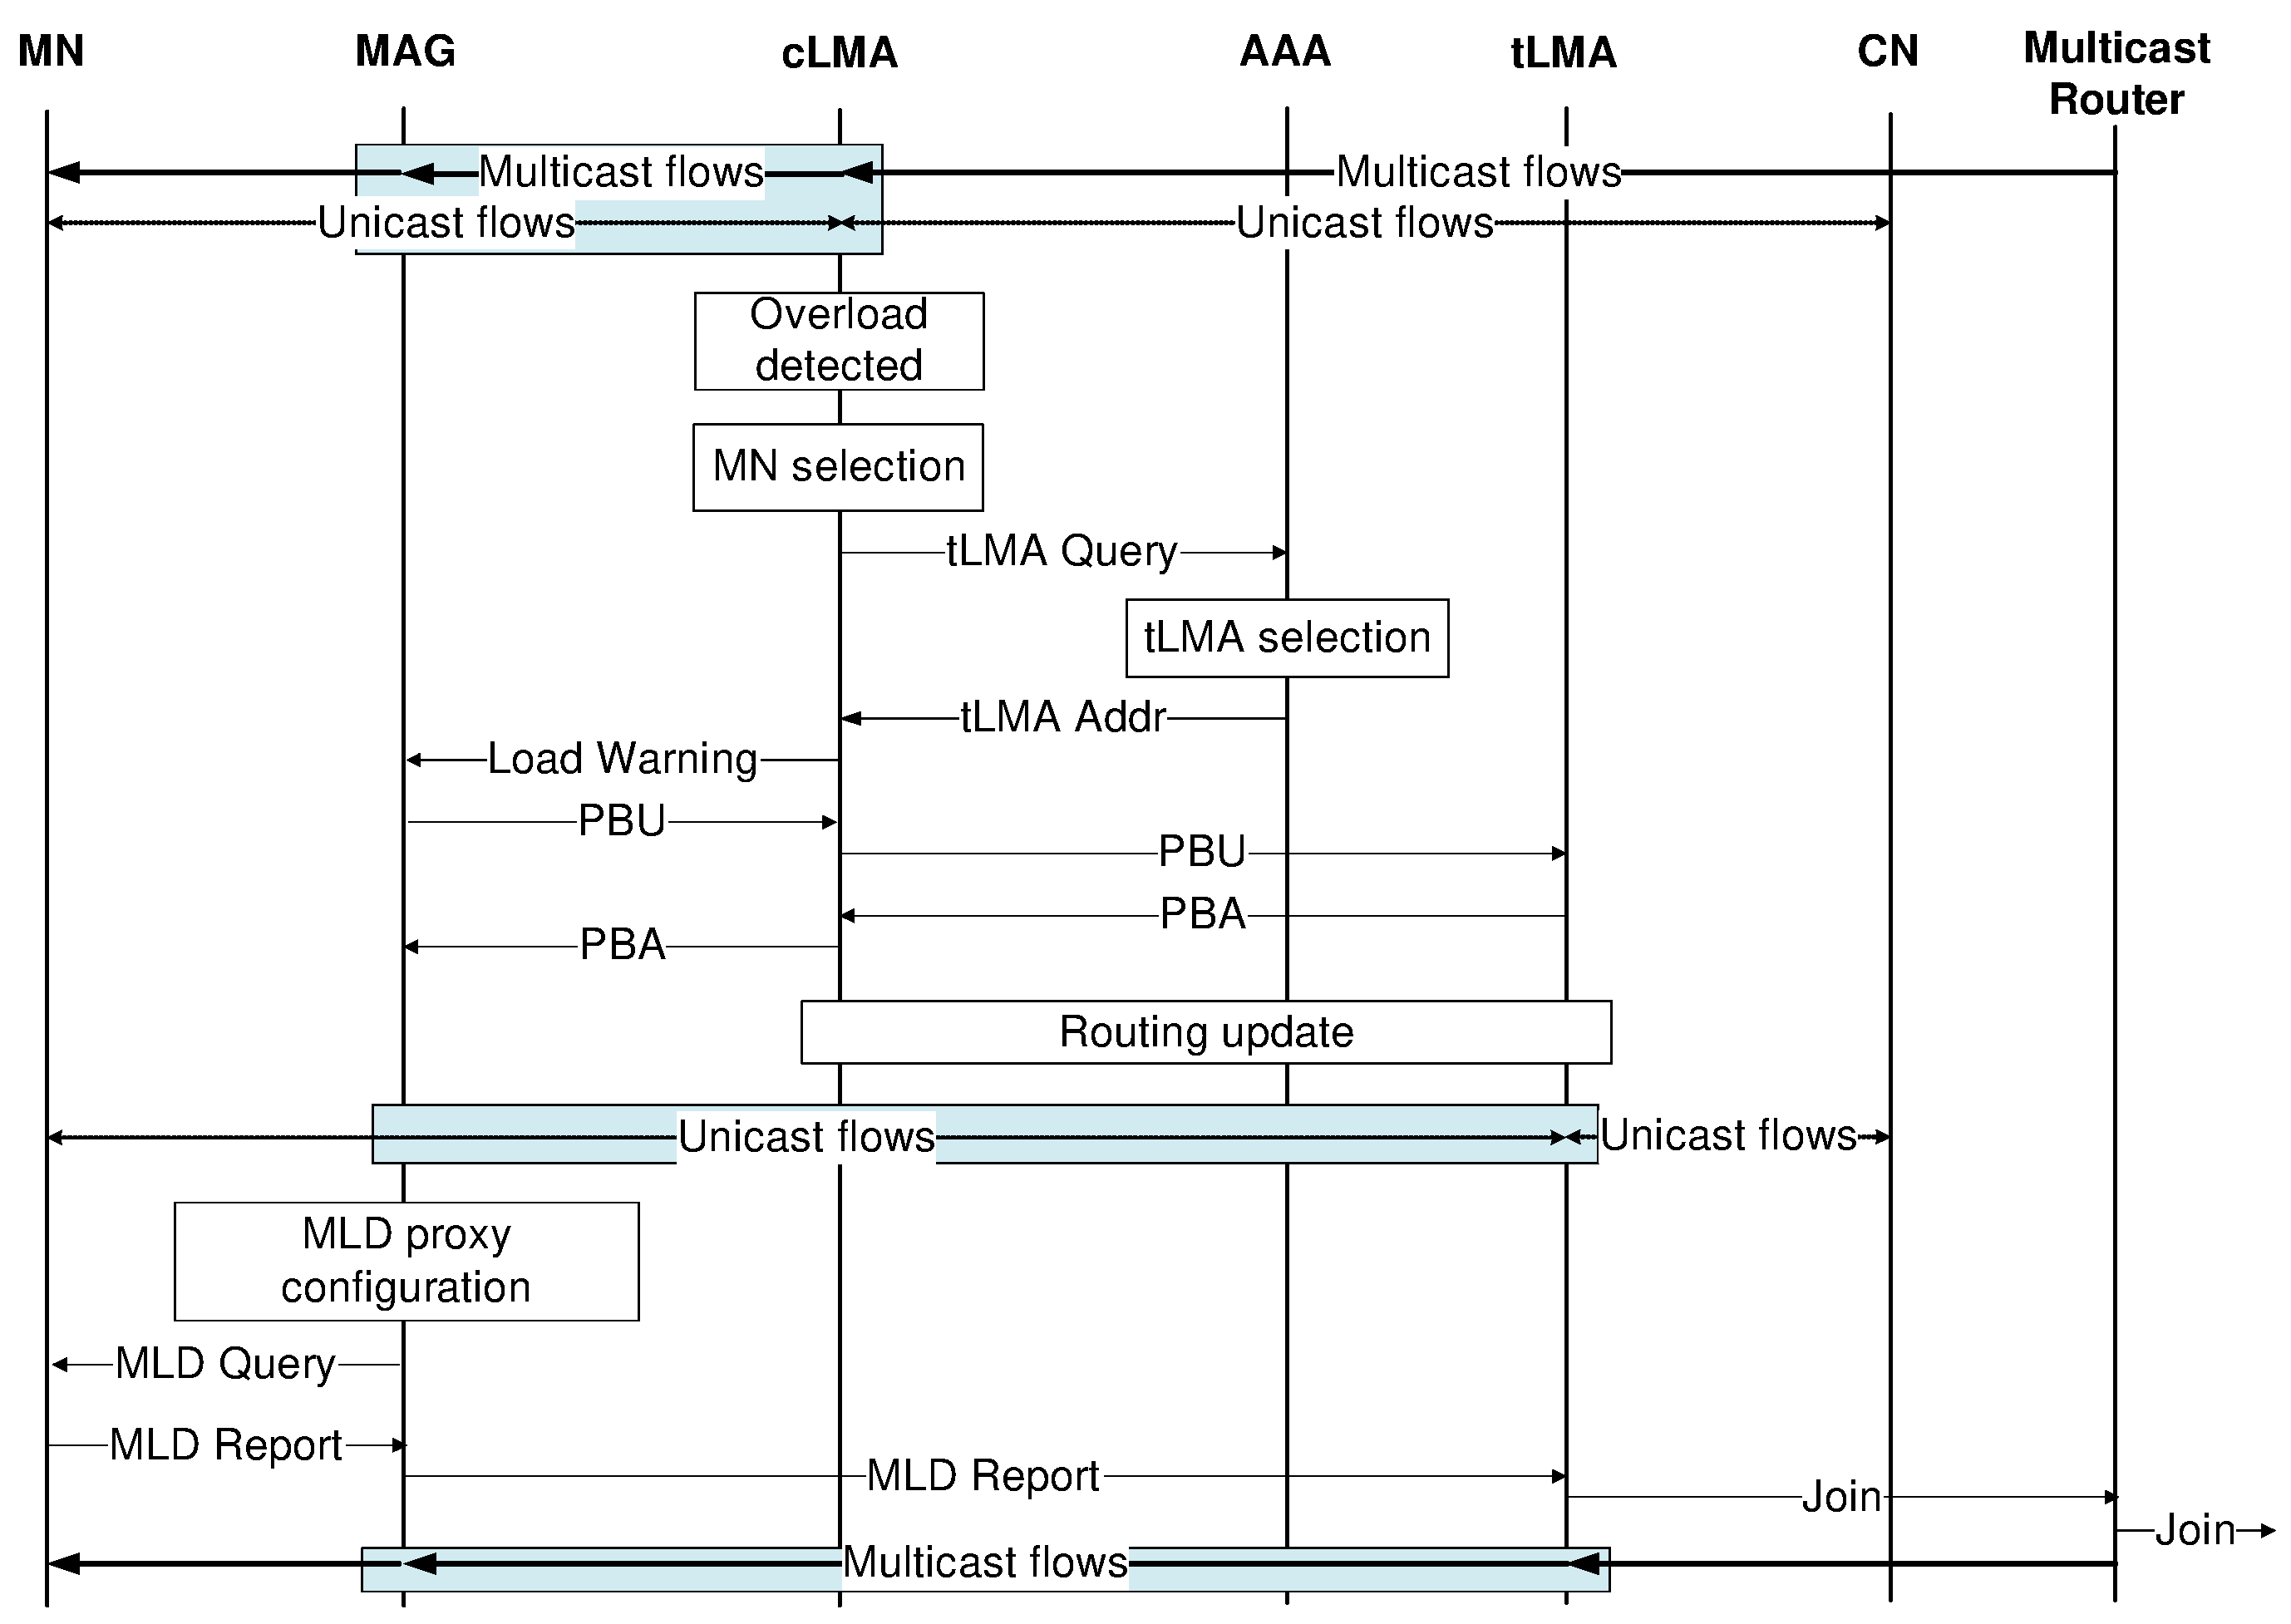
\includegraphics[width=0.70\textwidth]{./Part2/Chapter5/figures/reactive_MN_flow.eps} 
    \caption[Multicast considerations in the reactive-MN load balancing approach.]{Multicast considerations in the reactive-MN approach.}
     \label{fig:reactive_MN_flow}
  \end{center} 
\end{figure}

In the reactive-MN approach \cite{lb_lma,lb_mobility_session}, the LB will be triggered when the LMA load exceeds a specified threshold. The overloaded LMA will select one (or several) MN(s) to move to a less loaded LMA (called target LMA, or tLMA). The load information of all LMAs can be collected and managed at the authentication, authorization and accounting (AAA) server which then selects the tLMA among the LMAs in the domain. The PBU/PBA messages then are exchanged between the current LMA (cLMA) and the tLMA allowing the tLMA to serve as a new mobility anchor of the MN. This approach allows the network to adapt to the current situation. Thus, it may give a better performance e.g., distributing load among LMAs and increasing the reliability. Since the LMA plays the role of the mobility anchor for the MN, changing LMA during the mobility session could impact the selected MN’s ongoing sessions. For this reason, this change is not recommended by the IETF \cite{runtime_lma,lma_discovery}. In addition, the existing proposals only consider the ongoing sessions as the unicast ones. How the LB works with the multicast is still an open question.
 
To support multicast in a PMIPv6 domain, the multicast router (MR) and the MLD proxy function need to be deployed at the LMA and the MAG, respectively \cite{RFC_6224}. In the base solution, a listener always receives the multicast traffic from its LMA via the LMA-MAG tunnel. As stated earlier, several procedures need to be executed in order to allow the MAG to continue receiving the traffic (from the tLMA). As a result, it experiences a noticeable service disruption for the ongoing multicast channels. Additional mechanisms (e.g., MLD proxy peering function \cite{multicast_source}) are required to reduce the service disruption time. 

If there is more than one listener (including the selected one) associated with the cLMA and subscribing to the same multicast channel, the cLMA will continue forwarding this channel. Consequently, moving the MN cannot help significantly reduce the LMA load, especially when the load generated by this MN is mainly from this channel. The total load of all LMAs may also be increased since the tLMA may need to join the channel. In addition, as the LMA selection algorithm does not take multicast into account, the tLMA may not support the multicast capability. In other words, the multicast service cannot be guaranteed at the tLMA. Also, since many proxy instances are installed at MAG, it may cause the tunnel convergence problem.   

\section{Multicast-based Load Balancing Solution}\label{ch7:solution}
In this section, at first, some criteria to select the appropriate LMA and multicast session for the LB purpose will be discussed. Two different approaches of the multicast-based solution i.e., the proactive-multicast (or MAG-initiated) and the reactive-multicast (or LMA-initiated) approach are then considered. In the former case, LB will be invoked when an MN starts a new multicast session to select a suitable LMA to serve this session. In the latter case, LB will be executed when an LMA is overloaded by selecting a multicast session to move to the less loaded one. It can be done thanks to an extension to MLD proxy to support multiple upstream interfaces \cite{multiple_upstreams}. In this case, only one proxy instance is deployed at MAG with multiple upstream interfaces being configured towards different LMAs. As a result, the MN can receive the multicast traffic from a less loaded LMA, while obtaining the unicast traffic from its LMA. Further information can be found in \cite{Thinh_elsevier_LB, Thinh_ICNC}.
\paragraph{Target LMA Selection}
Target LMA selection is first based on the channel policy which is defined by the operators (if exist). Otherwise, the LMA selection relies on the following policies (from high to low priority):  i) The least loaded LMA among the (not overloaded) LMAs having the multicast forwarding state for this channel should be selected; and ii) The LMA with the lowest load in the domain should be selected. The selection policies come from the fact that if the channel is already available at the selected LMA (target LMA, or tLMA) with a negligible increase of load, the tLMA can forward this channel to the MAG \cite{developing_ip_multicast}. To do so, a new logical entity, the so-called load balancing controller (LBC), has been introduced. This entity collects and manages the load state information of all LMAs in the domain. It is also responsible for the LMA selection. 
Upon the location of the LBC, three different schemes can be considered as below:
\begin{itemize}
\item{Centralized LBC entity}: The functionality of the LBC is responsible by a central entity, called C-LBC. 
This entity is similar to the notion of rfLMA as described in \cite{runtime_lma}. The LMAs periodically report their current load to the C-LBC by using an extension to the PBA/PBU message with the load information \cite{runtime_lma}. The C-LBC can be co-located with the AAA server.
\item{Distributed LBC function on the LMAs}: The LBC function is executed in a distributed manner among the LMAs. Each LMA maintains a so-called Load Table which includes load information of all LMAs in the PMIPv6 domain. Each LMA periodically exchanges its load information with each other in the domain, for example, by setting a common multicast group for all LMAs.
\item{Distributed LBC function on the MAGs}: In this case, the load of all LMAs is collected and stored at the MAGs. The MAG can obtain the current load of the associated LMA by using an extension of PBU/PBA messages or an extension of the Heartbeat message with the load information \cite{lb-802.11}. 
\end{itemize}

Without loss of generality, this chapter only considers the first scheme. As all LMAs periodically report their workload to the C-LBC, the frequency of the workload report should be carefully examined as the trade-off between the precision of the load state and the signaling/processing overhead. One possible solution is that the LMA only reports its workload when its load exceeds/is lower than a certain load level. 

\paragraph{Multicast Session Selection}
The multicast session can be selected following some criteria: i) To reduce the potential impact on the ongoing session, the real-time and delay-sensitive session should not be selected. However, if all sessions are the real-time and delay-sensitive ones, the session with the highest data rate should be selected; and ii) The session requiring the highest data rate with the smallest number of subscribed listeners should be selected. It is noted that to better select LMA, the LMA selection algorithm should take the expected load of the selected multicast session into account.
%\vspace{-0.1in}
\subsection{Load Balancing in the Proactive-Multicast Approach}
\begin{figure}[h!] 
 \begin{center} 
 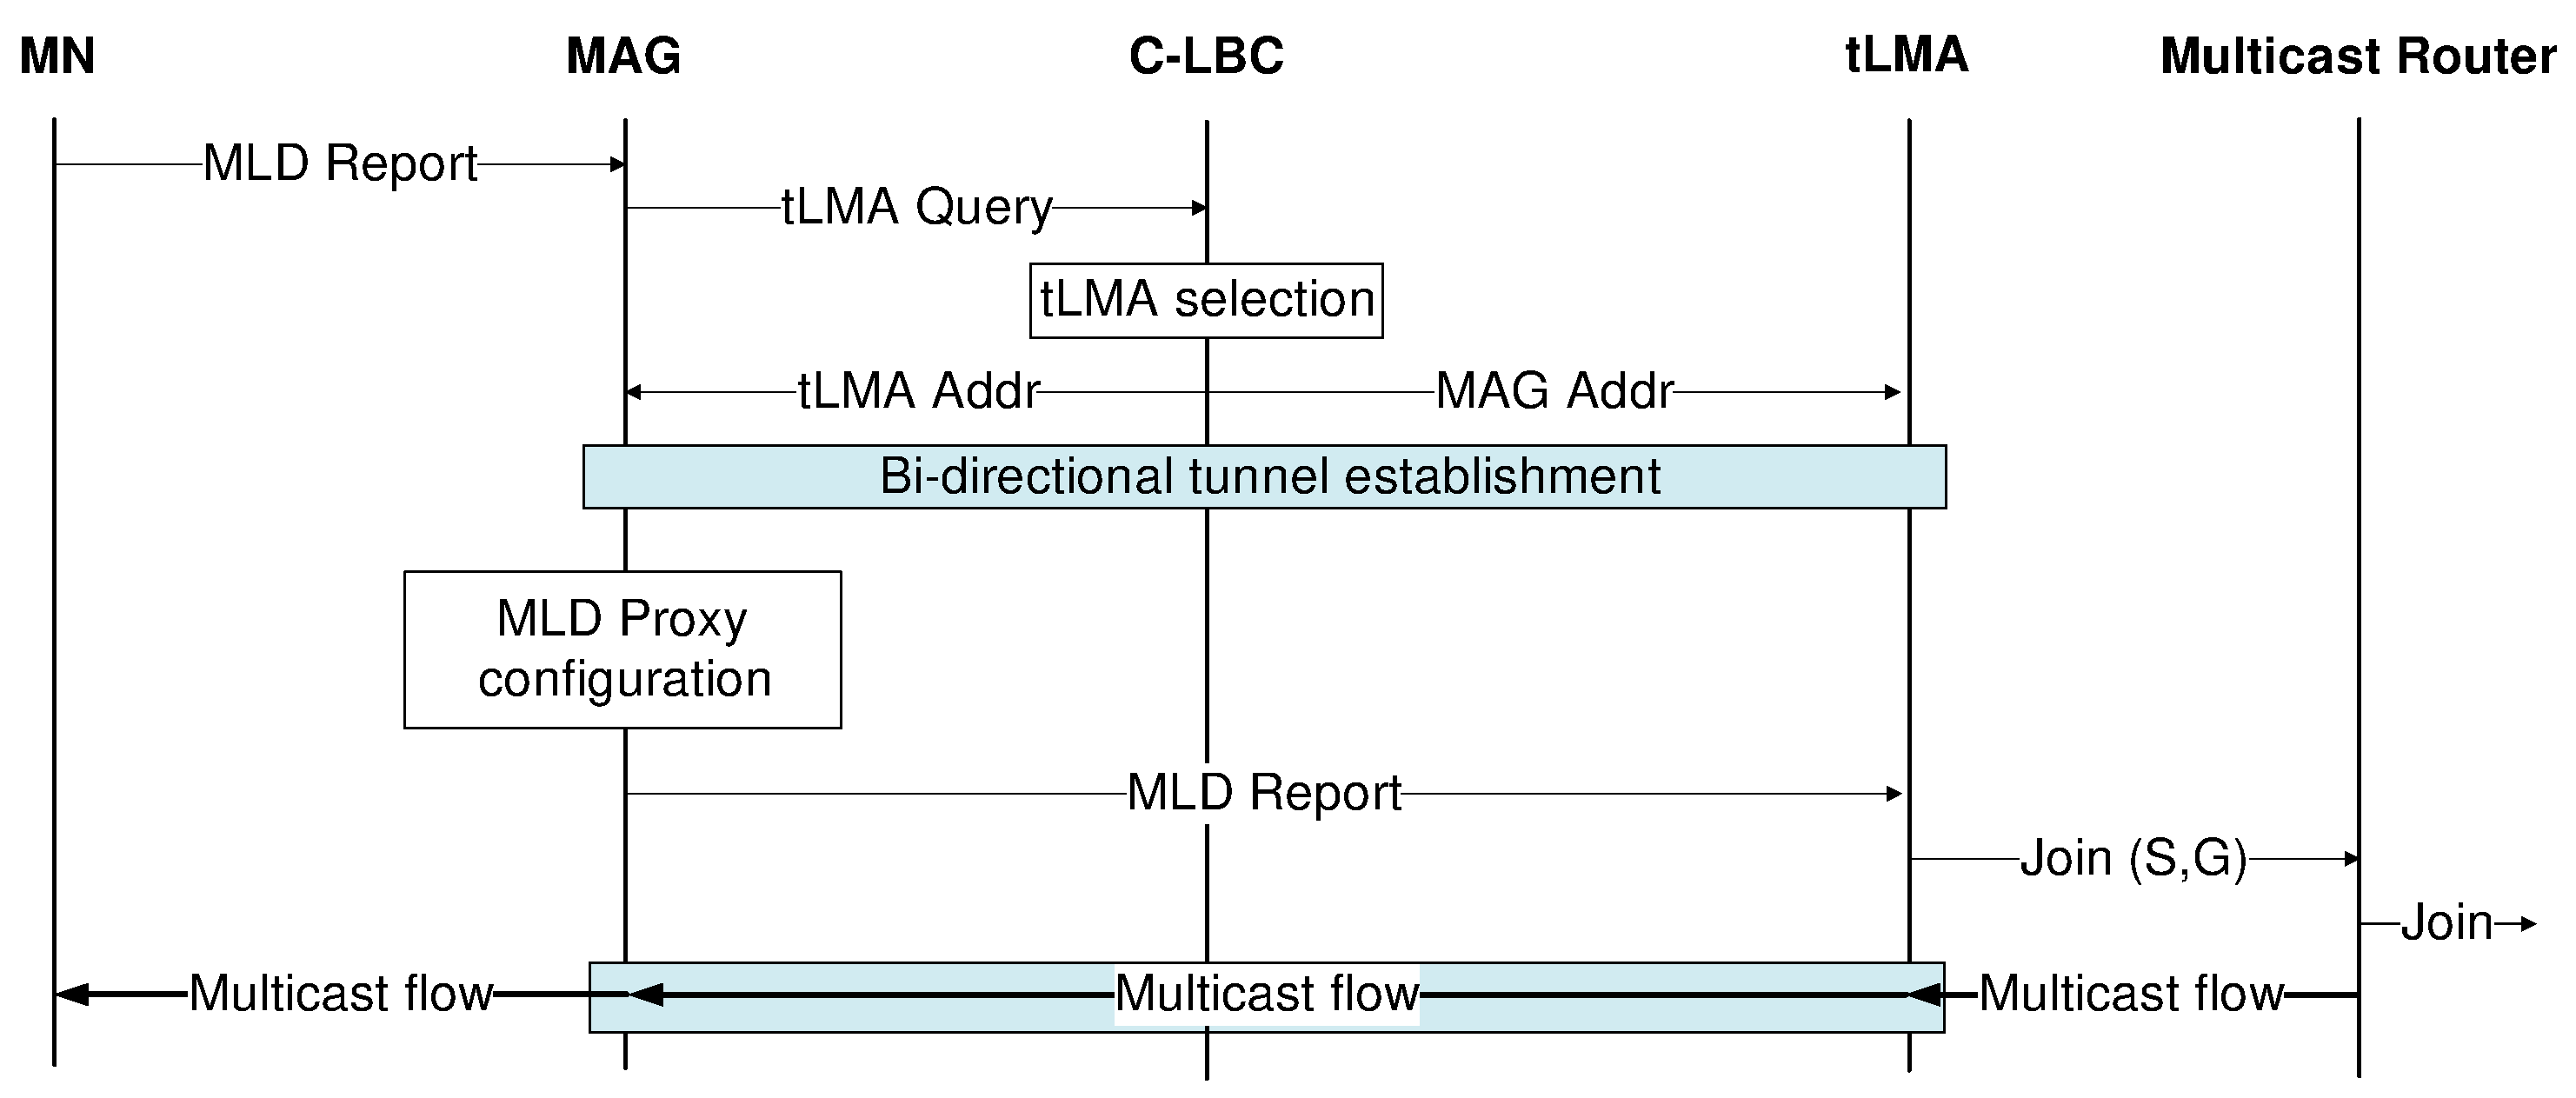
\includegraphics[width=0.65\textwidth]{./Part2/Chapter5/figures/c7_proactive_multicast.eps} 
    \caption[The proactive-multicast load balancing approach.]{Proactive-multicast approach.}
    \label{fig:proactive_multicast}
  \end{center} 
\end{figure}
The signaling procedure for the proactive-multicast (MAG-initiated) approach is illustrated in Fig.~\ref{fig:proactive_multicast}. When a registered MN wishes to subscribe to a multicast channel and this channel is available at the current MAG, the MAG will forward it directly to the MN. Otherwise, it will contact the C-LBC to get the address of an LMA (following the criteria as stated earlier), which can be served as the multicast anchor point for this session. After joining the channel via the tLMA, the MAG can receive the multicast packets and forwards them to the MN. Note that the communication between the MAG and the C-LBC can be done by extending the Remote Authentication Dial In User Service (RADIUS) protocol for PMIPv6 \cite{radius}.

\subsection{Load Balancing in the Reactive-Multicast Approach}
\begin{figure}[h!] 
 \begin{center} 
 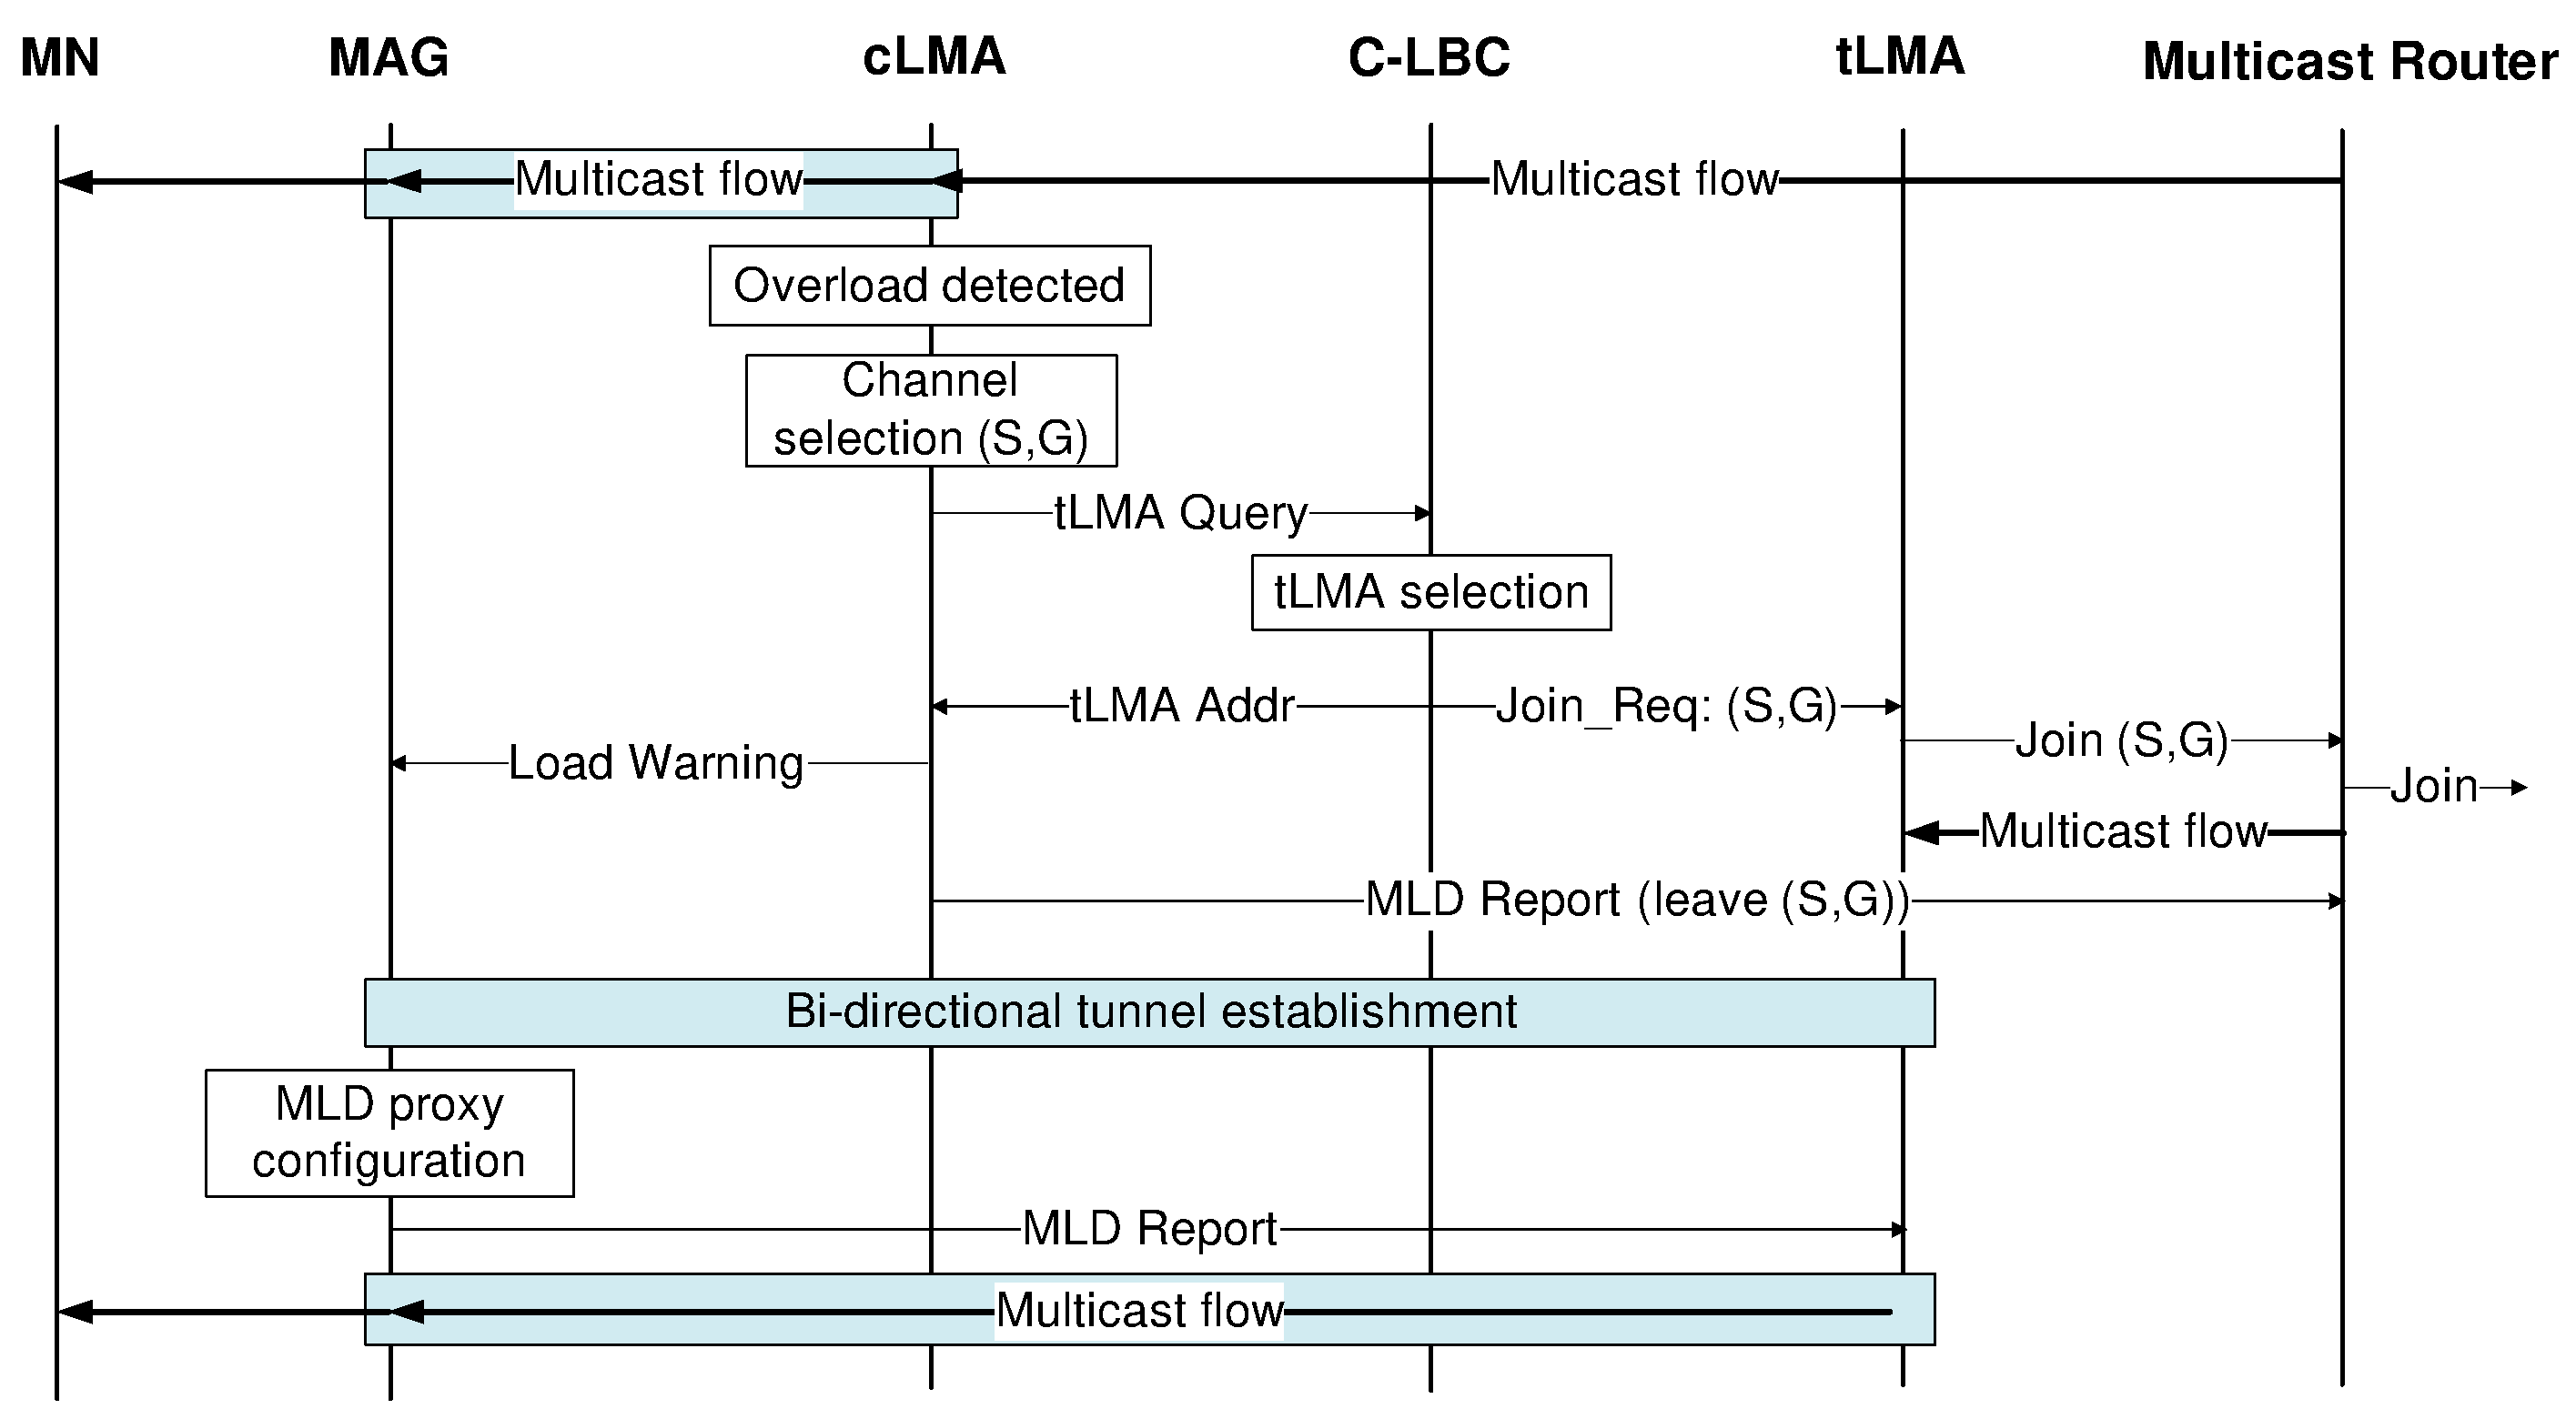
\includegraphics[width=0.70\textwidth]{./Part2/Chapter5/figures/reactive_multicast.eps} 
    \caption[The reactive-multicast load balancing approach.]{Reactive-multicast approach.}
        \label{fig:reactive_multicast}
  \end{center} 
\end{figure}

Fig.~\ref{fig:reactive_multicast} shows the signaling procedure for the reactive-multicast (LMA-initiated) approach. When an LMA (cLMA) is overloaded (its load exceeds a certain threshold), a multicast session will be selected to move from this LMA to a less loaded one (tLMA).
After obtaining the tLMA address from the C-LBC, the cLMA sends the tLMA's address and the selected multicast session information to all related MAGs via a load-warning message (e.g., using an extension to the Update Notification message (UNP) \cite{update_notification}). The C-LBC also requests the tLMA to join the channel in advance to reduce the multicast service disruption. The MAG then sends an MLD Report to the tLMA to join the channel. Afterwards, the MAG can receive the multicast packets from the tLMA instead from the cLMA. In the meantime, the cLMA can leave this channel in order to lower its load.
\subsection{Handover Consideration}
\begin{figure}[h!] 
 \begin{center} 
 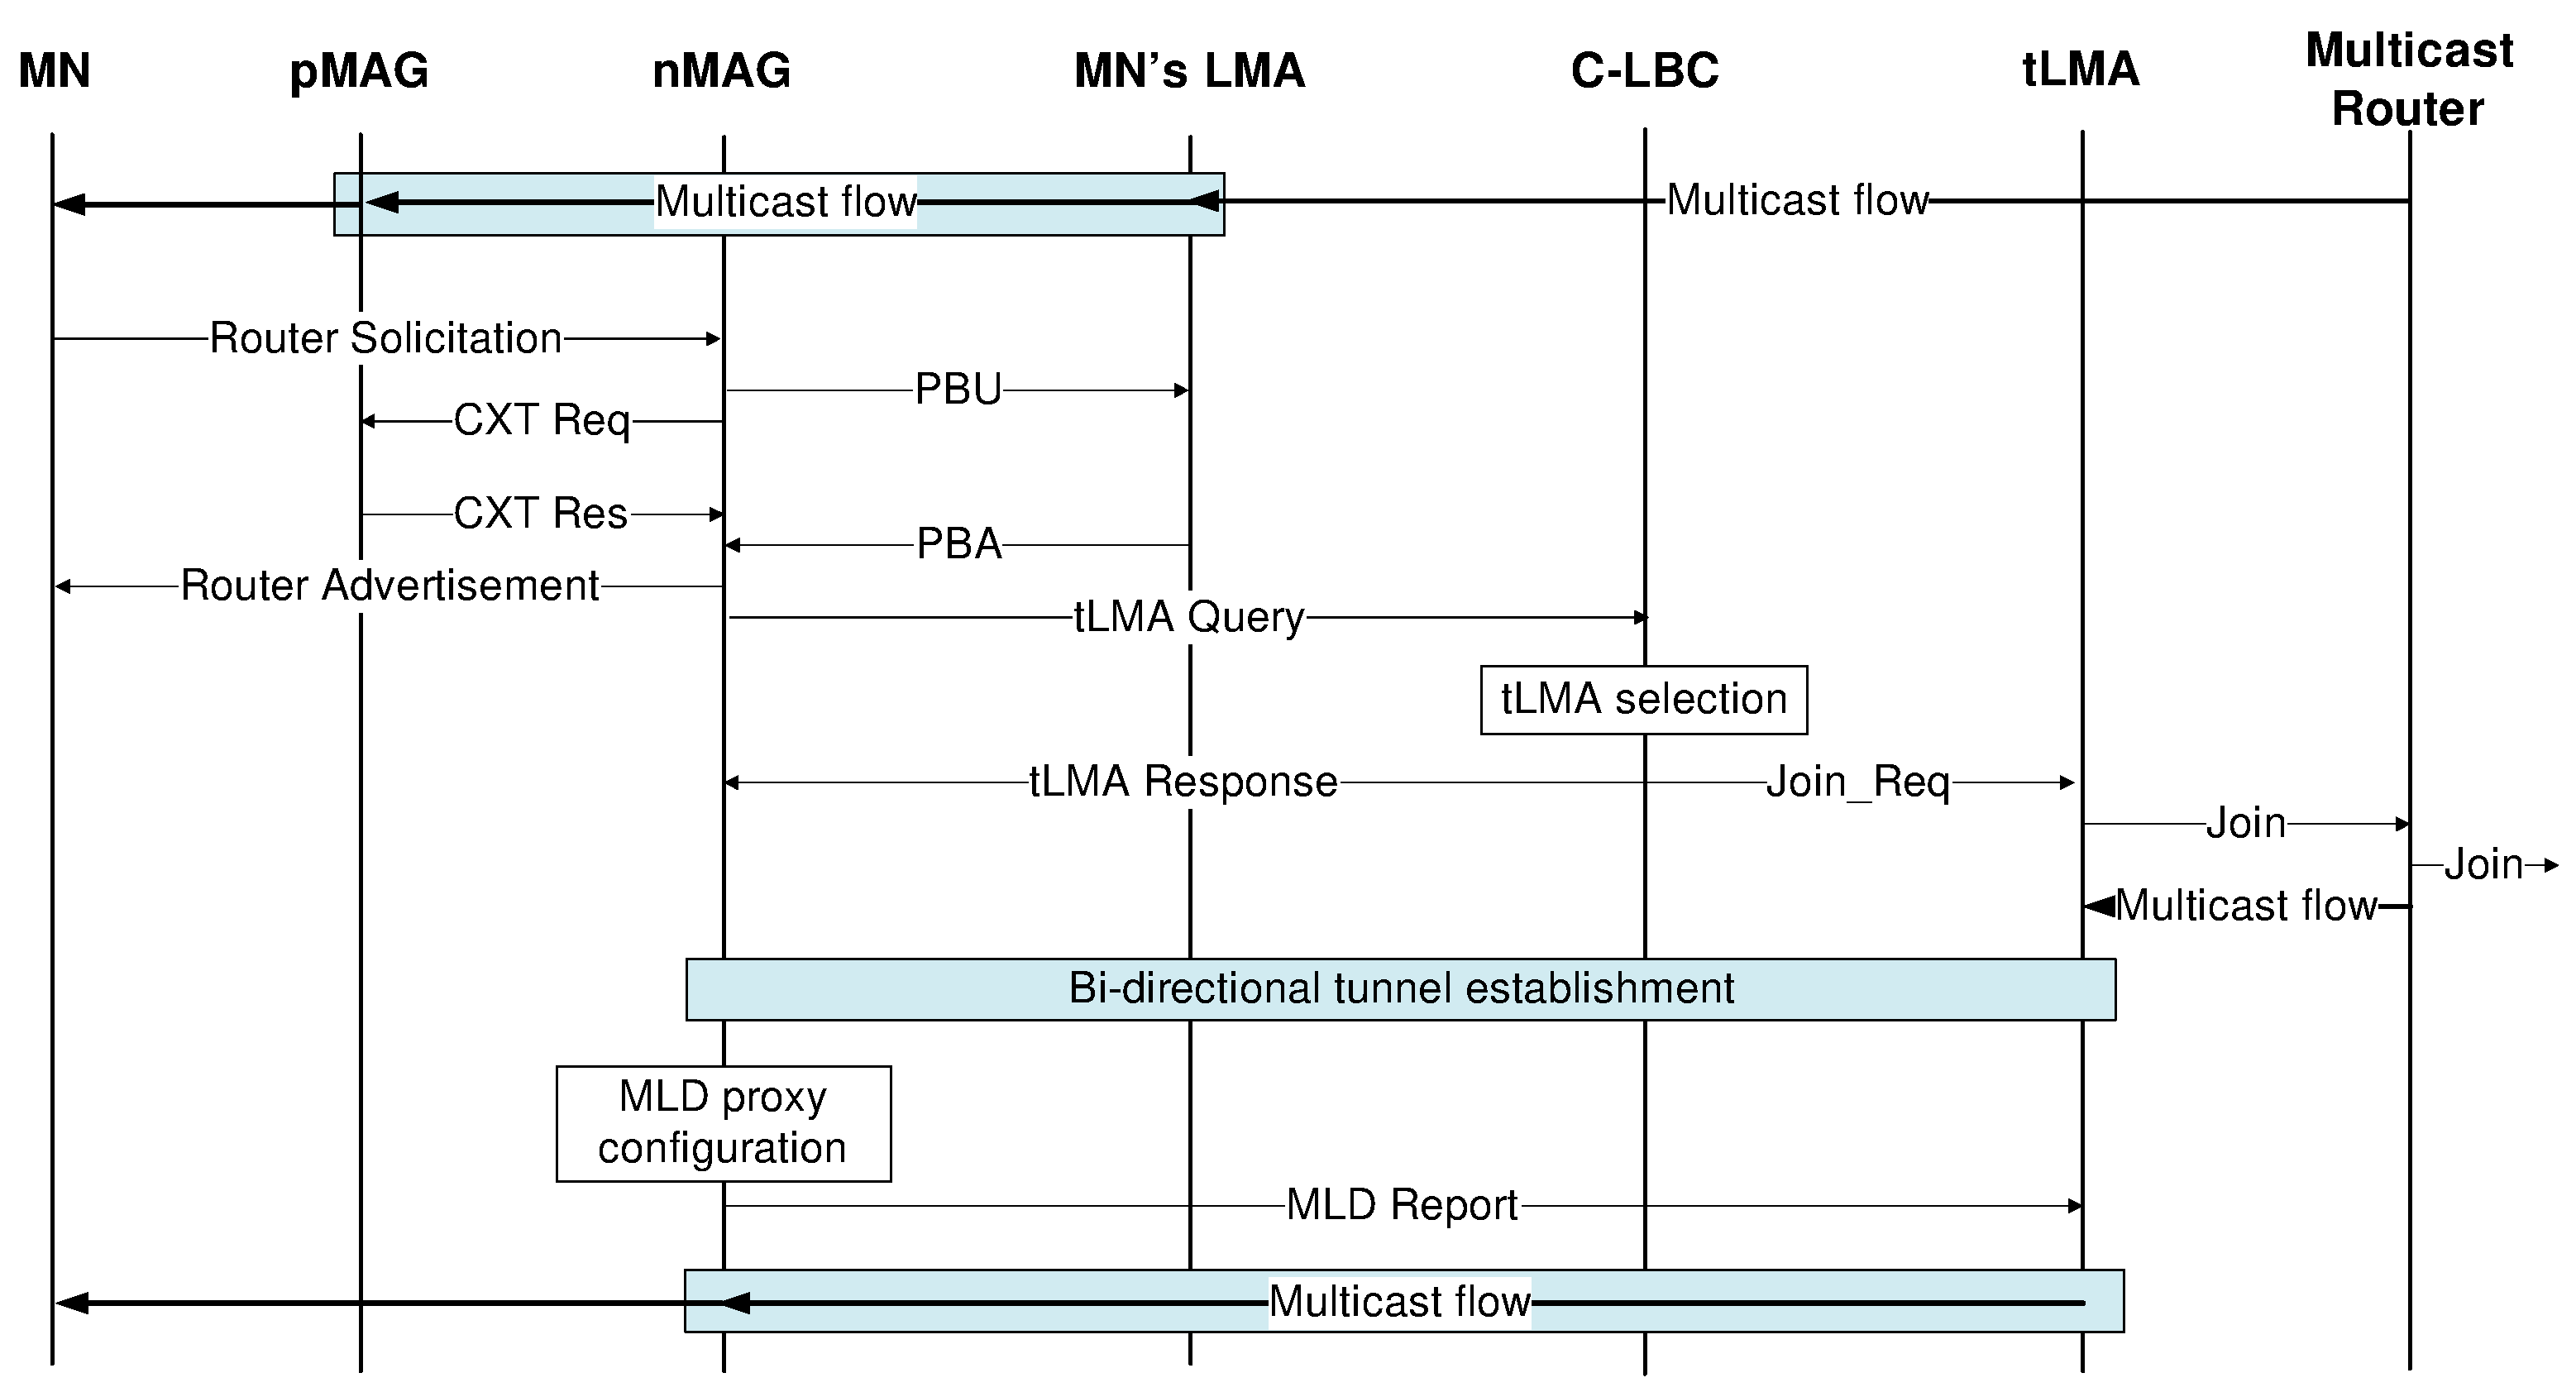
\includegraphics[width=0.70\textwidth]{./Part2/Chapter5/figures/c7_handover_multicast.eps} 
    \caption[Load balancing-related signaling when a node performs a handover in a PMIPv6 domain.]{Handover signaling with LB.}
        \label{fig:handover_multicast}
  \end{center} 
\end{figure}
As can be seen in Fig.~\ref{fig:handover_multicast}, if the MN performs a handover between two MAGs, the normal PMIP operation will be executed to update the routing information at the MN's LMA and the new MAG. Then, the similar process as for the new multicast session at the new MAG will be undertaken to select the appropriate LMAs to serve the ongoing multicast channels.

\section{Performance Analysis}\label{ch7:performance_analysis}
In this section, at first, we will highlight the different load factors imposed on the LMA. Based on that the comparison will be conducted between the reactive-MN and the reactive-multicast approach regarding their efficiency. The multicast service disruption time will also be considered. 
\subsection{Load Analysis}
As stated previously, to support multicast in a PMIPv6 domain, the multicast router (MR) function and the MLD proxy function \cite{RFC_6224} need to be deployed at the LMA and the MAG, respectively. All multicast traffic passes through the MAG-LMA tunnel, accordingly. As such, the load of the LMA comes from two main parts: the load from the typical LMA's tasks ($L_{lma}^{lma}$) and the load from the MR's tasks ($L^{mr}_{lma}$). It is noted that a minor amount of load which is imposed by the background processes (e.g., system processes) is ignored in our analysis.   
Thus, we have\\
\begin{equation}
L_{lma}^{(.)} = L_{lma}^{lma} + L_{lma}^{mr}.
\end{equation}

As a typical LMA, it performs three main logic functions: mobility routing (processing the unicast traffic from/to the associated MNs), location management (processing PBU/PBA, updating binding cache, maintaining tunnel, etc.) and home network prefix (HNP) allocation \cite{PMIPv6}.
As a result, the $L_{lma}^{lma}$ comes from three main parts $L_{lma}^{mor}$, $L_{lma}^{lm}$, and $L_{lma}^{hal}$ corresponding to these logic functions. The $L_{lma}^{mor}$ and $L_{lma}^{hal}$ depend on all the unicast sessions of the registered MNs, and the new MN arrival rate ($\lambda_{n}$), respectively.  While $L_{lma}^{lm}$ depends on the number of registered MNs ($n$) and the new MN arrival rate ($\lambda_{n}$). Hence, they are given by
\begin{eqnarray}
    L_{lma}^{mor}&{} ={}& \sum_{i=1}^{n} \sum_{j=1}^{u_{i}} L_{mn_{i}}^{j},\\
    L_{lma}^{hal}&{} ={}& \lambda_{n} L_{hal},\\
     L_{lma}^{lm}&{} ={}& (n+ \lambda_{n}) L_{lm},
\end{eqnarray}

where $L_{mn_{i}}^{j}$ is the load offered by the unicast flow j of the MN$_{i}$; $L_{lm}$ and $L_{hal}$ are the unit load generated when the LMA performs the location management and HNP allocation for an MN. 

Regarding the multicast router role, the $L_{lma}^{mr}$ can be split into three main contributions corresponding to three functions: packet replication ($L_{mr}^{pr}$), reverse path forwarding (RPF) recalculation ($L_{mr}^{rpf}$,) and state maintenance function ($L_{mr}^{sm}$) \cite{developing_ip_multicast}. The $L_{mr}^{pr}$ is the total load from all the multicast channels which are available at the LMA, and defined as 
 
\begin{equation}
L_{mr}^{pr} = \sum_{i=1}^{m} L_{mc_{i}},
\end{equation}
where $L_{mc_{i}}$ is the load of channel $MC_{i}$.
Note that the multicast router can replicate the data for multiple outgoing interfaces with almost the same level of load compared to that for one interface (or the unicast traffic with the same characteristics e.g., packet size and data rate) \cite{developing_ip_multicast}.  

Let us now consider the different load factors which can be used as the parameters to select the appropriate LMA such as: processor capacity (CPU), number of supported sessions, number of registered MNs, and bandwidth. Accordingly, we assign each factor with a weighting variable which reflects the selected load factors. We then obtain\\
\begin{equation}
L_{lma}^{(.)} = \alpha \left( n + \lambda_{n} \right) L_{lm} + \beta  \lambda_{n} L_{hal} + \gamma \sum_{i=1}^{n} \sum_{j=1}^{u_{i}} L_{mn_{i}}^{j}  + \delta L_{mr}^{rpf} + \theta  L_{mr}^{sm} + \rho  \sum_{i=1}^{m} L_{mc_{i}}. 
\label{lma_load}
\end{equation}

where $\alpha, \beta, \gamma, \delta, \theta$, and $\rho$ are weighting factors (in the interval [0,1]). For example, if the load is defined as the number of registered MNs, only two factors $L_{lma}^{lm}$ and $L_{lma}^{hal}$ are taken into account. In this case, the values of $\gamma, \delta, \theta, \rho$ should be set to 0. LMA load is given as\\
\begin{equation}
L_{lma}^{(.)} = \alpha \left( n+ \lambda_{n} \right) L_{lm} + \beta \lambda_{n} L_{hal}. 
\label{eg:load_mn}
\end{equation}

As a result, the impact of the number of sessions as well as the session's data rates on the LMA load are ignored. Similarly, if the load is considered as the number of sessions, the $L_{lma}^{mor}$ and $L_{mr}^{pr}$ are taken into consideration, in which the load of each session is identical. Thus, $\alpha, \beta, \delta$, and $\theta$ should be set to 0. Eg.~(\ref{lma_load}) becomes  \\
\begin{equation}
L_{lma}^{(.)} = \gamma \sum_{i=1}^{n} \sum_{j=1}^{u_{i}} L_{mn_{i}}^{j} + \rho \sum_{i=1}^{m} L_{mc_{i}}. 
\end{equation}

Again, the impact of the session's data rate is ignored. However, it is obvious that a high data rate session puts much more load on the LMA than the low data rate one. Therefore, they cannot be treated equally. In this chapter, we consider the sessions with different characteristics have different impact on the load. 

In order to evaluate the load distribution among LMAs in different approaches, we use Jain's Fairness Index \cite{jain-index}. Let L denote the set of LMAs in the domain: $L=\lbrace LMA_{1},..,LMA_{l}\rbrace$, where l is the number of LMAs. According to \cite{jain-index}, the fairness index can be computed by\\
\begin{equation}
FI = \dfrac{(\sum_{i=1}^{l} L_{lma}^{(i)})^{2}}{l \cdot \sum_{i=1}^{l} (L_{lma}^{(i)})^{2}},
\end{equation} 
where $L_{lma}^{(i)}$ is the load of the $LMA_{i}$ (i=1,..,l).
The fairness index ranges from $\frac{1}{l}$ to 1, in which the higher index indicates more fair situation. Ideally, when the load is equally distributed among LMAs, the fairness index is 1.
    
\subsection{Multicast Service Disruption Consideration}
\begin{figure}[tb!] 
  \begin{center} 
    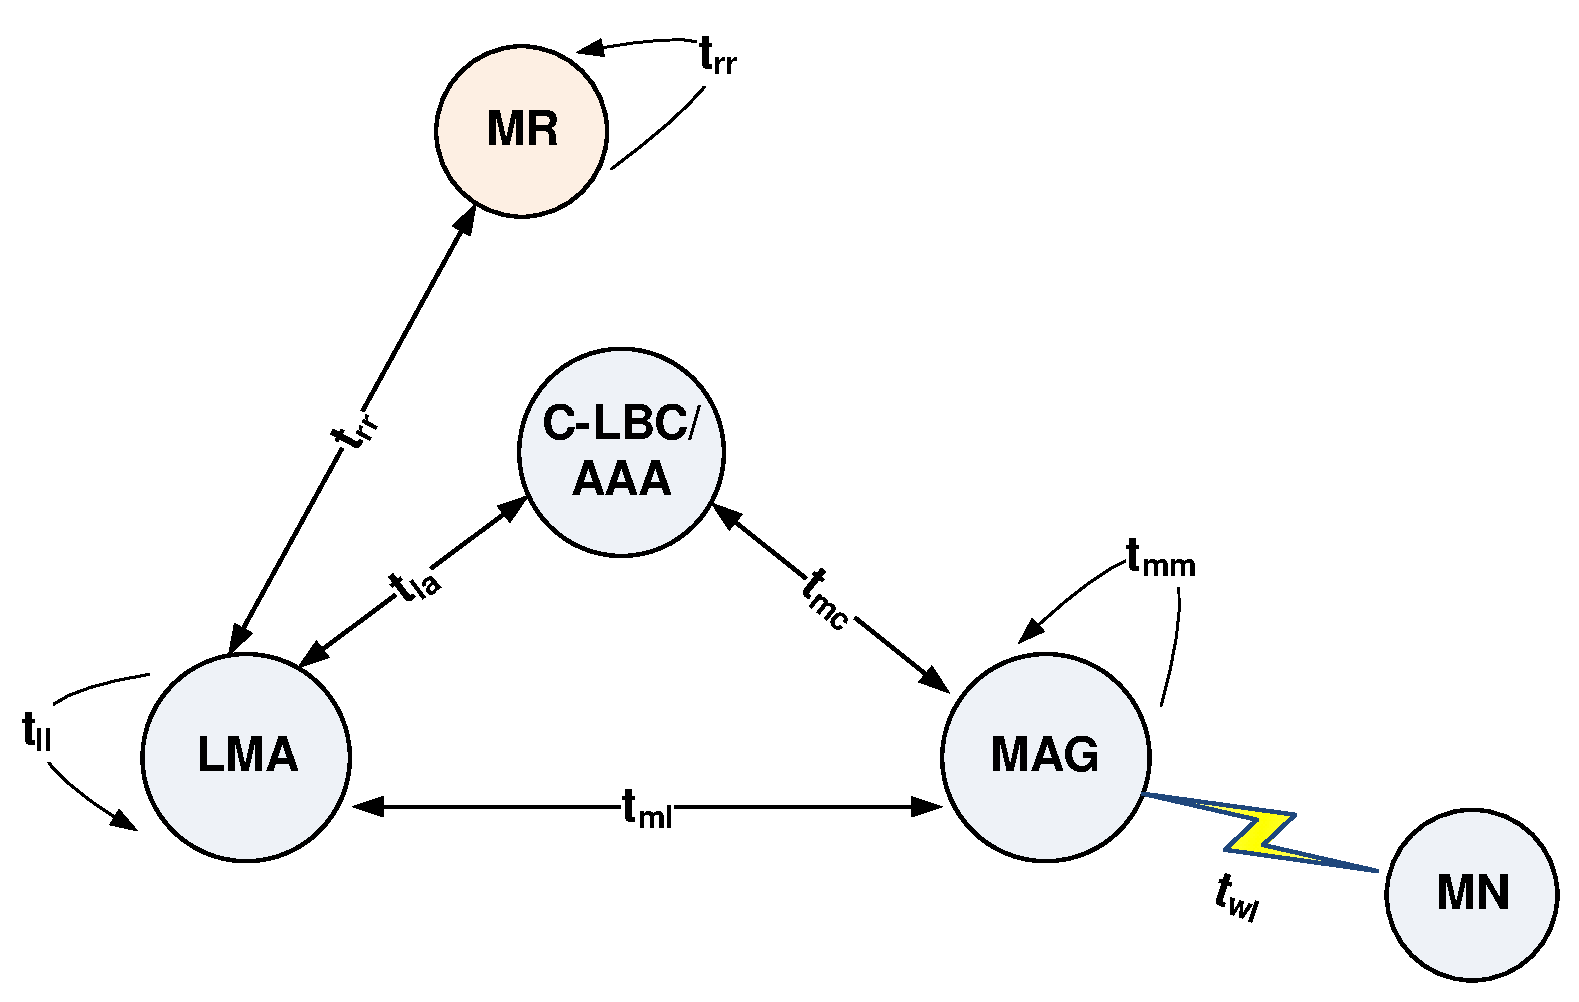
\includegraphics[width=0.52\textwidth]{./Part2/Chapter5/figures/topology_analysis.eps} 
    \caption[Reference network topology for multicast service disruption analysis: from the load balancing perspective]{Reference network topology.}
    \label{fig:topology_analysis}
  \end{center} 
\end{figure}
In the reactive-MN and the reactive-multicast approach, the changing LMA of an MN (listener) may cause the service disruption of the ongoing multicast sessions. The multicast service disruption time is defined as a period when a listener cannot receive the multicast packets. Fig.~\ref{fig:topology_analysis} shows a reference topology for performance analysis. The delay factors consisting of the total
delay are defined as follows:
\setlength \abovedisplayskip{-1pt}
\vspace{-0.1in}
\begin{itemize}
\itemsep 0.07em
\item $t_{mm}$: the delay between two MAGs.
\item $t_{ml}$: the delay between MAG and LMA.
\item $t_{mc}$: the delay between MAG and C-LBC.
\item $t_{la}$: the delay between LMA and AAA/C-LBC.
\item $t_{ll}$: the delay between two LMAs. 
\item $t_{rr}$: the delay between two MRs (between LMA and MR).
\item $t_{wl}$: the delay between MAG and listener (MN) (wireless connection).
\item $t_{join}$: the delay time an MR needs to join a multicast channel (including processing time and PIM Join transmission time).
\item $t_{qrd}$: the query response delay which is the interval between the moment when the MN receives an MLD Query and replies with an MLD Report \cite{MLDv2}.
\item $t_{cv}$: the routing convergence time which reflects the time to update the new anchor location of the selected MN's prefix.
\end{itemize}

In the reactive-MN approach, as can be seen in Fig.~\ref{fig:reactive_MN_flow}, the service disruption time ($SD$) can be calculated from the moment when the cLMA sends a PBU to the tLMA until the moment when the MN receives the first multicast packet from the tLMA. Let $d_{join}$ and $d_{delivery}$ denote the time needed for the tLMA to join and get the first multicast packet for this channel (from a router which already had the multicast forwarding state for this group, namely intersection MR or IMR), respectively. Assuming that $n_{mr}$ is the average number of hops between tLMA and IMR, we have 
\begin{equation}
d_{join} = n_{mr} t_{join},
\end{equation}
\begin{equation}
d_{delivery} = n_{mr} t_{rr}.
\end{equation}

Thus, the service disruption time in the reactive-MN approach is given by\\
\begin{equation}
SD_{R\_MN} = 2t_{ll} + 3t_{ml} + 3t_{wl} + t_{qrd} + n_{mr} t_{join} + n_{mr} t_{rr} + t_{cv}. 
\label{eq:r_mn}
\end{equation}

Via the utilization of the peering function (PF) in the reactive-MN approach, the time needed for the MLD proxy instance at the MAG to obtain the multicast subscription information can be ignored. Consequently, the service disruption can be calculated as\\
\begin{equation}
SD_{R\_MN\_PF} = 2t_{ll} + 3t_{ml} + t_{wl}  + n_{mr} t_{join} + n_{mr} t_{rr} + t_{cv}.
\label{eq:r_mn_pf}
\end{equation}

Similarly, the service disruption time in the reactive-multicast approach is computed from the moment when the cLMA sends a load warning message to the MAG until the moment when the MN receives the multicast traffic (see Fig.~\ref{fig:reactive_multicast}).\\
\begin{equation}
SD_{R\_M} = max \{2t_{ml}, n_{mr} t_{join} + n_{mr} t_{rr}\} + t_{ml} + t_{wl}.
\label{eq:r_m}
\end{equation}

Also, as seen in Fig.~\ref{fig:handover_multicast}, the service disruption during handover (multicast handover latency) when applying the multicast-based LB mechanism is expressed as\\
\begin{multline}
SD_{HO} = D_{L2} + 2t_{wl} + max \{2t_{ml}, 2t_{mm}\} + t_{mc} \\+max \{t_{mc} +t_{ml}, t_{la} + n_{mr} t_{join} + n_{mr} t_{rr}\} + t_{ml}.
\label{eq:ho}
\end{multline}

\section{Experimentation}\label{c7:experiment}
From the LB perspective, this section will present two separate experiments. At first, we will show in general how the different factors affect the load of an LMA. We will then evaluate the performance of the multicast-based solution in comparison with the MN-based solution and the pure-PMIP environment (without any load balancing mechanism) by using a near-to-real testbed. It is noted that, at this stage, we only focus on the case where the traffic is dominated by the multicast traffic. In addition, the load is defined as the CPU utilization rate and the performance metric is the load distribution among the LMAs. From the multicast perspective, this section will present the numerical results for the service disruption time analysis given in the previous section. 

\subsection{Experimentation Setup and Scenarios Description}
\begin{figure}
\centering
\subfloat[]{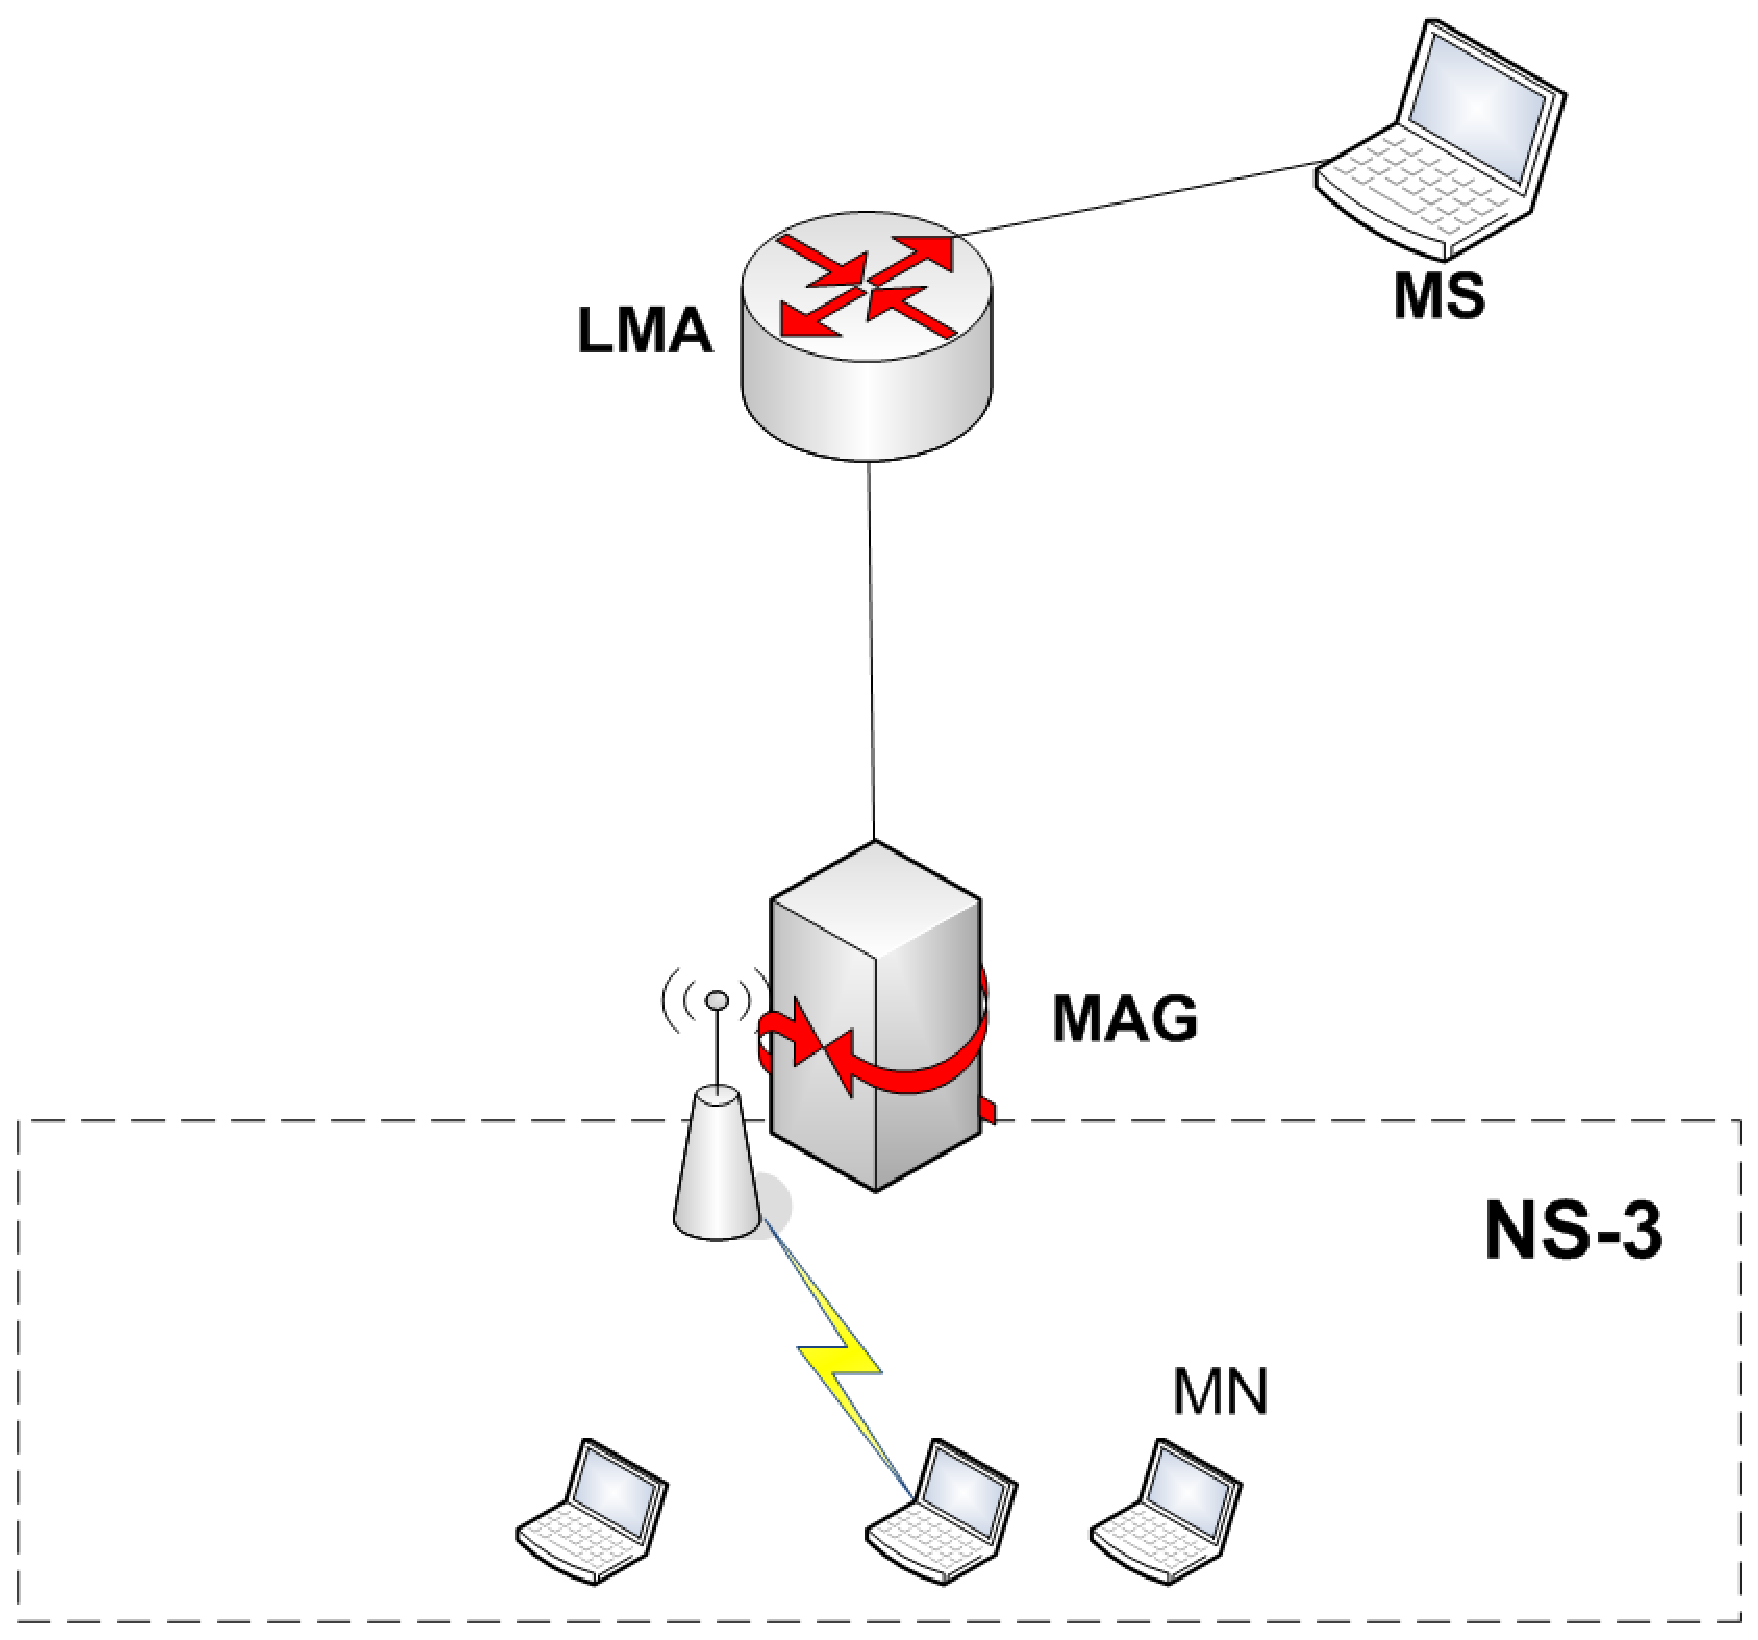
\includegraphics[width=0.35\textwidth]{./Part2/Chapter5/figures/testbed-measurement.eps} \label{fig:testbed-measurement}}\,
\subfloat[]{\includegraphics[width=0.47\textwidth]{./Part2/Chapter5/figures/testbed.eps}\label{fig:testbed-multicast}}
\caption[Testbeds for load balancing mechanisms. ]{Testbeds: (a) Experiment 1, (b) Experiment 2}
\label{fig:testbed}
\end{figure}

As illustrated in Fig.~\ref{fig:testbed}, the testbed is deployed as similar as in Chapter \ref{ch:multicast_PMIP}. The PMIP entities (LMA, MAG) and the multicast sources (MSs) are the virtual machines while the access points (APs) and MNs, which play the role of a multicast listener, are NS-3 nodes. During the experimentation, the LMA load is collected by using a performance measurement tool e.g., \textit{mpstat}\footnote{http://linuxcommand.org/man\_pages/mpstat1.html}. To improve the credibility of the experiment results, the LMA load was collected every one second during 360 seconds in each experiment. 

To generate the multicast traffic, several tools can be used e.g., \textit{Iperf} \cite{iperf} and \textit{MINT} \cite{mint} (and \textit{mcfirst}\footnote{mcfirst command: http://manpages.ubuntu.com/manpages/precise/man1/mcfirst.1.html}). 
For example, in case of \textit{Iperf},  the following Linux commands can be used: \\
\textit{Source\# Iperf -s -u -B ff08::1 -V -i 1}\\
\textit{Listener\# Iperf -c ff08::1 -V -u -T 32 -t 100 -i 1 -l 67B -p 12345}

In case of using \textit{MINT} and \textit{mcfirst}: \\
\textit{Source\# ./mint -s -p 1234 -n 1000 -6 -t 12 ff08::2}\\
\textit{Listener\# mcfirst -6 -I eth0 ff08::1 1234}
\subsubsection{Impact of Different Load Factors} 
To show the impact of different factors on the LMA load, the first experiment used a testbed composing of one LMA, one MAG (and one AP), and one MS, as described in Fig.~\ref{fig:testbed-measurement}. Then two experiment scenarios are defined. The scenario 1 aims at demonstrating the case when the load takes into account only the number of MNs. The number of MNs associated with the LMA will be varied from 1 to 150 (Due to the limitation of the testbed, it can only support upto 150 MNs). The binding registration signaling for these MNs occurred within a small interval (50s) which almost represents the worst case scenario.  The scenario 2 shows the impact of unicast/multicast flow with different data rates on the LMA load. Thus, only one MN is required. At first, the MN subscribes to a multicast channel broadcasting by the MS. The LMA load will be measured when the flow's data rate is varied from 100 Kbps to 15 Mbps. Note that a standard definition video streaming typically runs at 3.75 Mbps while the high definition at 15 Mbps \cite{multicast-bandwidth}. The multicast flow is then replaced by the unicast one with the same data rate. The datagram size in both cases is kept constant at 67 bytes.
\subsubsection{Evaluation of the Multicast-based LB Mechanism}
The second experiment aims at evaluating the performance of the multicast-based solution in comparison with the MN-based and the pure-PMIP environment. At this stage, the experiment focuses on the case where the traffic is dominated by the multicast traffic. The performance evaluation metric is the load distribution among LMAs. This metric is selected since we could not achieve high system performance without fairly and efficiently utilizing the available network resources. The other metrics such as queuing delay and packet dropping probability will be left for future works. 

As illustrated in Fig.~\ref{fig:testbed-multicast}, the testbed is composed of one LBC, three LMAs, three MAGs (and three APs), three MSs, and 18 MNs. The C-LBC functionality is implemented by extending the LMA functionality. At the beginning, each multicast source $MS_{i}$ (i=1,2,3) broadcasts six multicast channels $C_{ij}$ (j=1,..,6) with identical traffic characteristics (400 Kbps). In the experiment, we use the same threshold value for all LMAs, for example, 85 percent of the CPU utilization rate. At first, the $MN_{ij}$ attaches to the $MAG_{i}$ and the $LMA_{i}$, respectively. The unicast flow is also created between each MN and the corresponding MS (100 Kbps). Two scenarios are then defined to evaluate the proactive-multicast and the reactive-multicast approach. 

In the scenario 1, six $MN_{1j}$ (j=1,..,6) join six multicast channels $C_{1j}$ (via $LMA_{1}$); $MN_{21}$ joins $C_{21}$ (via $LMA_{2}$); $MN_{31}$ and $MN_{32}$ join $C_{31}$, $C_{32}$ (via $LMA_{3}$), respectively. Three approaches are considered: the pure-PMIP, the proactive-MN and the proactive-multicast.
In the scenario 2, six $MN_{ij}$ (j=1,..,6) join three multicast channels (say $C_{i1}$, $C_{i2}$, $C_{i3}$) at the $LMA_{i}$ (i=1,2,3) (two MNs per channel, three channels at each LMA). Then the data rate of the existing multicast sessions as well as the number of sessions are varied to make the LMA load changes. For instance, at the $LMA_{1}$ the data rate of the channel $C_{11}$ and $C_{12}$ is increased with 800 Kbps and 1.2 Mbps, respectively. The channel $C_{21}$ (at $LMA_{2}$) and the channels $C_{31}$, $C_{32}$ (at $LMA_{3}$) are terminated. The results then are collected when the pure-PMIP, the reactive-multicast and the reactive-MN approach are applied.

\subsection{Experimental Results}
\subsubsection{Load Factors Measurement}
\begin{figure}[h!]
\centering
\subfloat[]{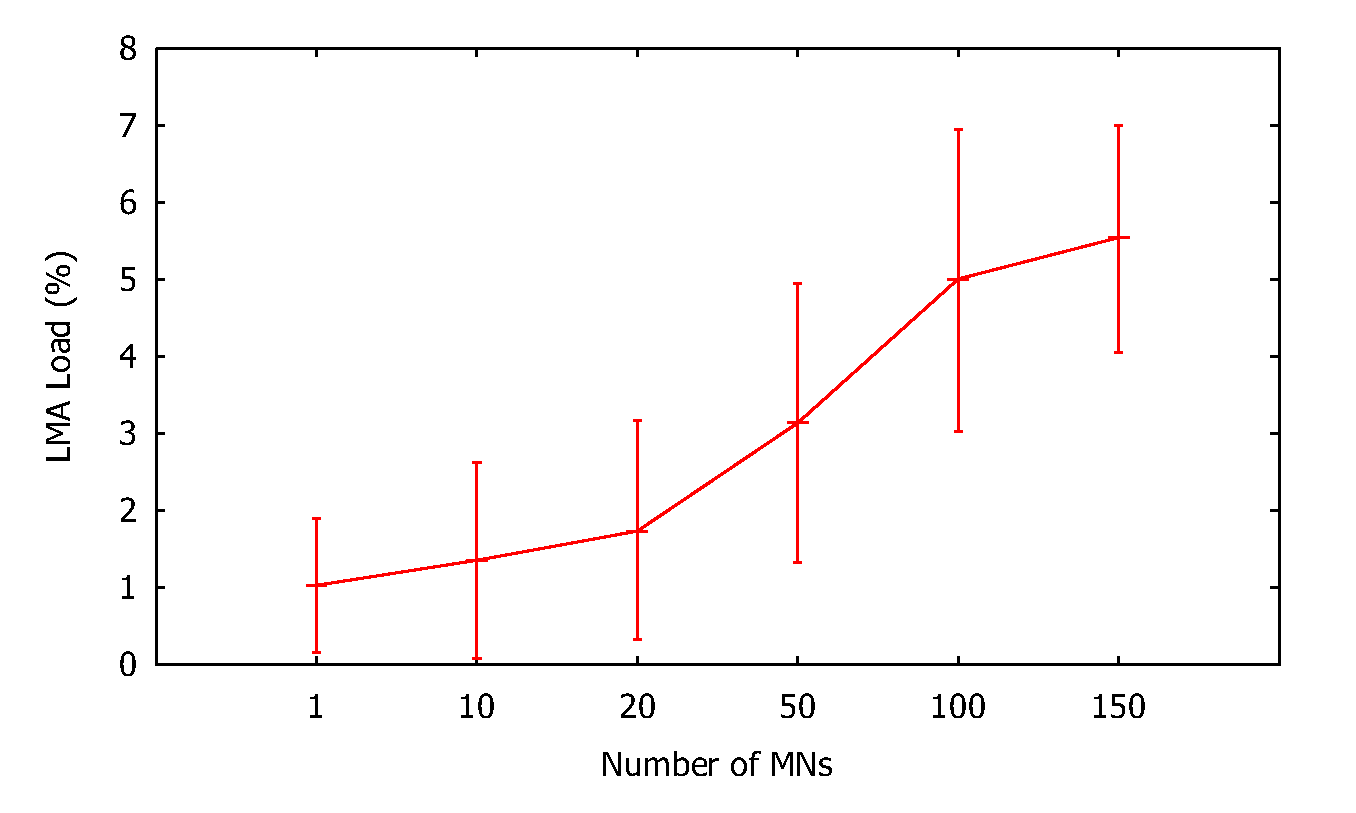
\includegraphics[width=0.47\textwidth]{./Part2/Chapter5/figures/lma_mn.eps} \label{fig:lma_mn}}\,\,\,\,\,\,
\subfloat[]{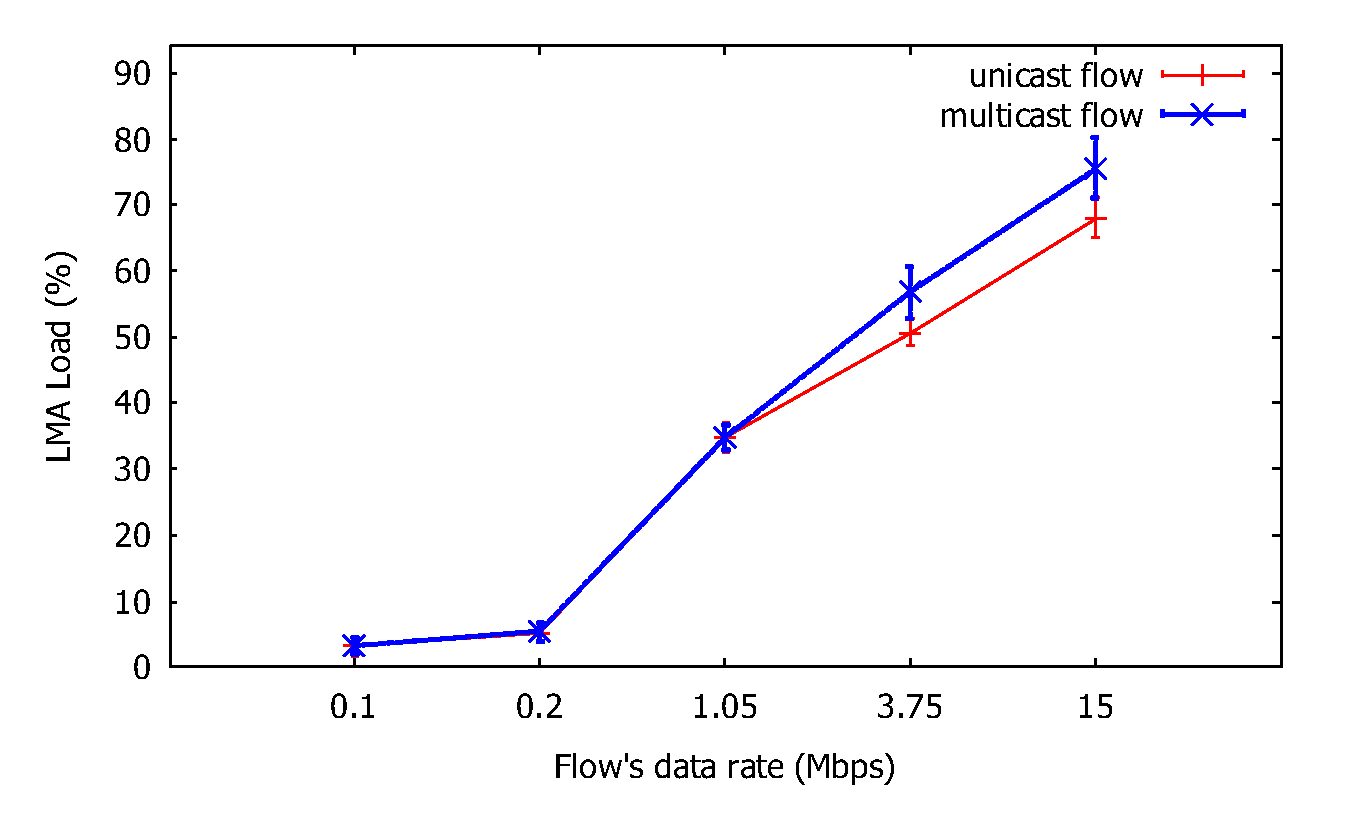
\includegraphics[width=0.47\textwidth]{./Part2/Chapter5/figures/unicast_multicast.eps}\label{fig:unicast_multicast}}
\caption[Load factors measurement.]{Experiment 1: (a) load .vs number of MNs, (b) unicast .vs multicast flow.}
\label{fig:experiment1}
\end{figure}
Fig.~\ref{fig:lma_mn} reports the average and standard deviation values of LMA load as a function of the number of MNs (scenario 1). In this case, the load is calculated according to Eq.~(\ref{eg:load_mn}). We also measure the load from background processes: (average, standard deviation) = (1.001\%, 0.888\%). We can observe that the load slightly increases when the number of MNs increases. Fig.~\ref{fig:unicast_multicast} illustrates the LMA load when the data rate of the multicast and unicast flow is varied (scenario 2). When the flow's data rate is low, the load imposed by the multicast and unicast flow is almost the same.  As the flow rate increases, the load offered by the multicast flow is higher than that by the unicast flow. As the experiment was conducted by using a very limited capacity machine, it requires about 75\% load to treat a high definition video flow (15 Mbps). 
It also could be observed that the load offered from a typical LMA's task with 150 MNs is similar to that from a low rate multicast flow (about 200 Kbps). Thus, it is obvious that the multicast/unicast flow is a crucial factor in terms of load put on the LMA. In other words, in a multicast-dominated domain, moving an MN from the overloaded LMA could not help reduce its load significantly. 
\subsubsection{Evaluation of the Multicast-based Load Balancing Solution}
Fig.~\ref{fig:fi_proactive} shows the FI value in the scenario 1. At the beginning, the load of all LMAs is almost the same. As a result, the FI value is very close to 1 (indicating that the load is almost shared among the LMAs). From the time the MNs subscribed to the multicast channels (at about 120s), the FI value is decreased rapidly in the pure-PMIP environment since the load is concentrated on the $LMA_{1}$. For instance, the $LMA_{1}$ becomes overloaded while the $LMA_{2}$ and $LMA_{3}$ are at low load. Since the LMA assignment is already done for the MNs, the FI value in the pure-PMIP can also be considered as that in the proactive-MN. We observed that the FI value in the multicast-based approach is always greater than that in the other cases. Also, the FI value is close to 1. It demonstrates that the multicast-based approach achieves a better load distribution among the LMAs. The reason is the proactive-multicast approach dynamically assigns the channel to the least loaded LMA at the time when the channel is started. 
\begin{figure}[h!]
\centering
\subfloat[]{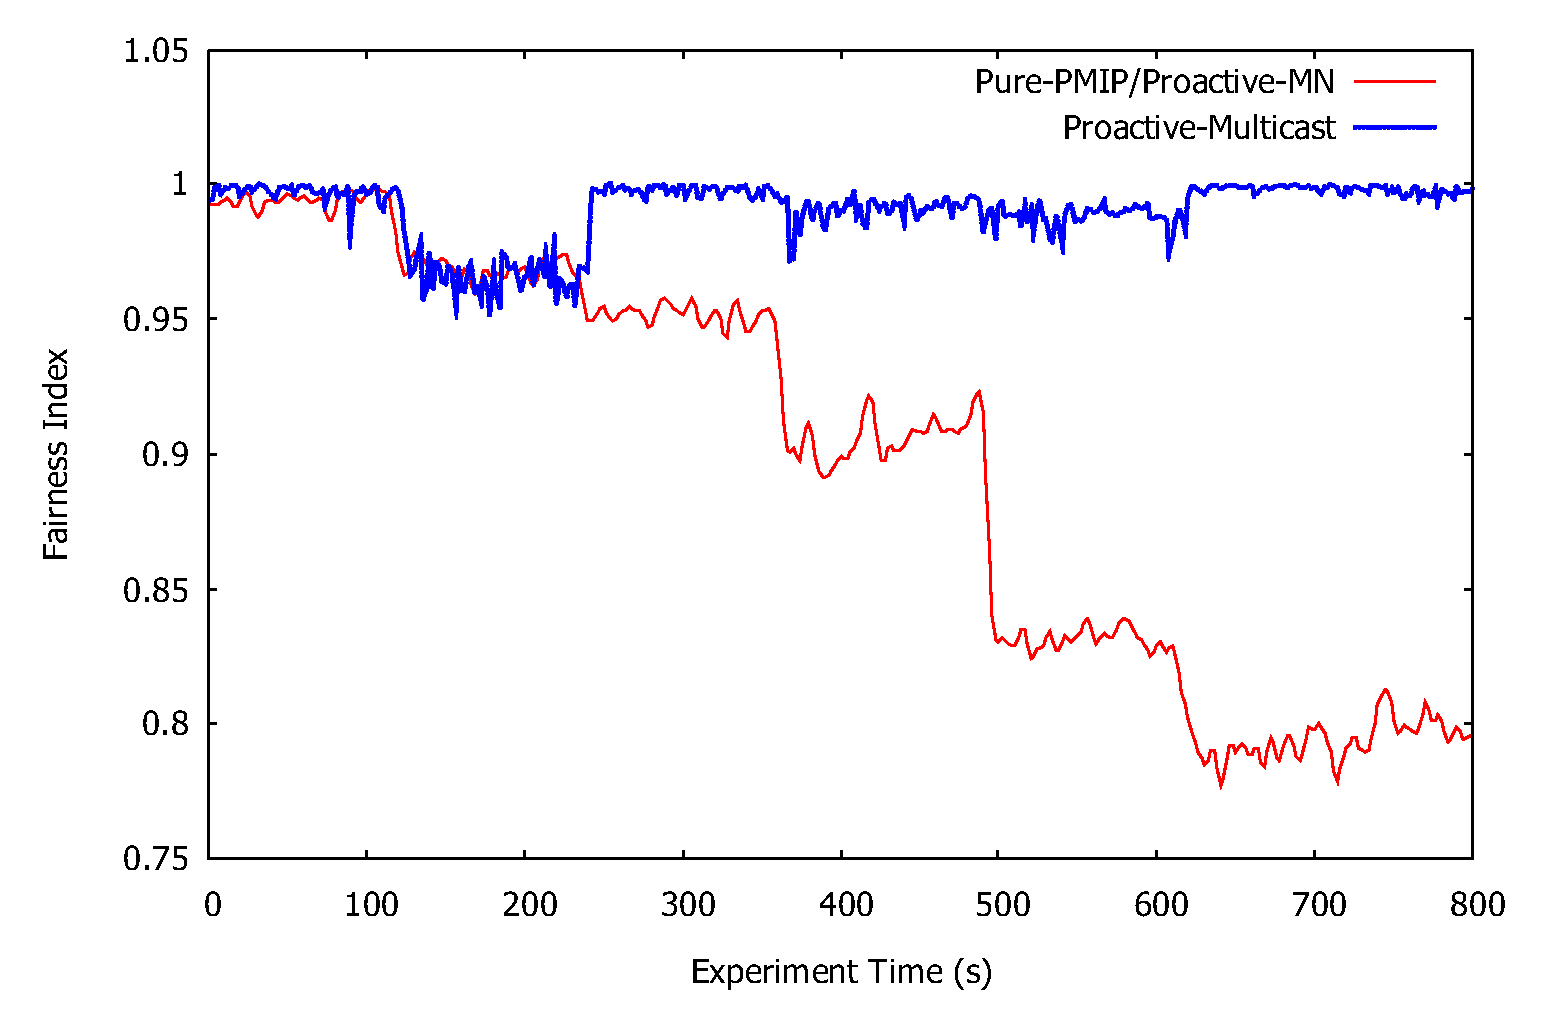
\includegraphics[width=0.47\textwidth]{./Part2/Chapter5/figures/fi_proactive.eps} \label{fig:fi_proactive}}\,
\subfloat[]{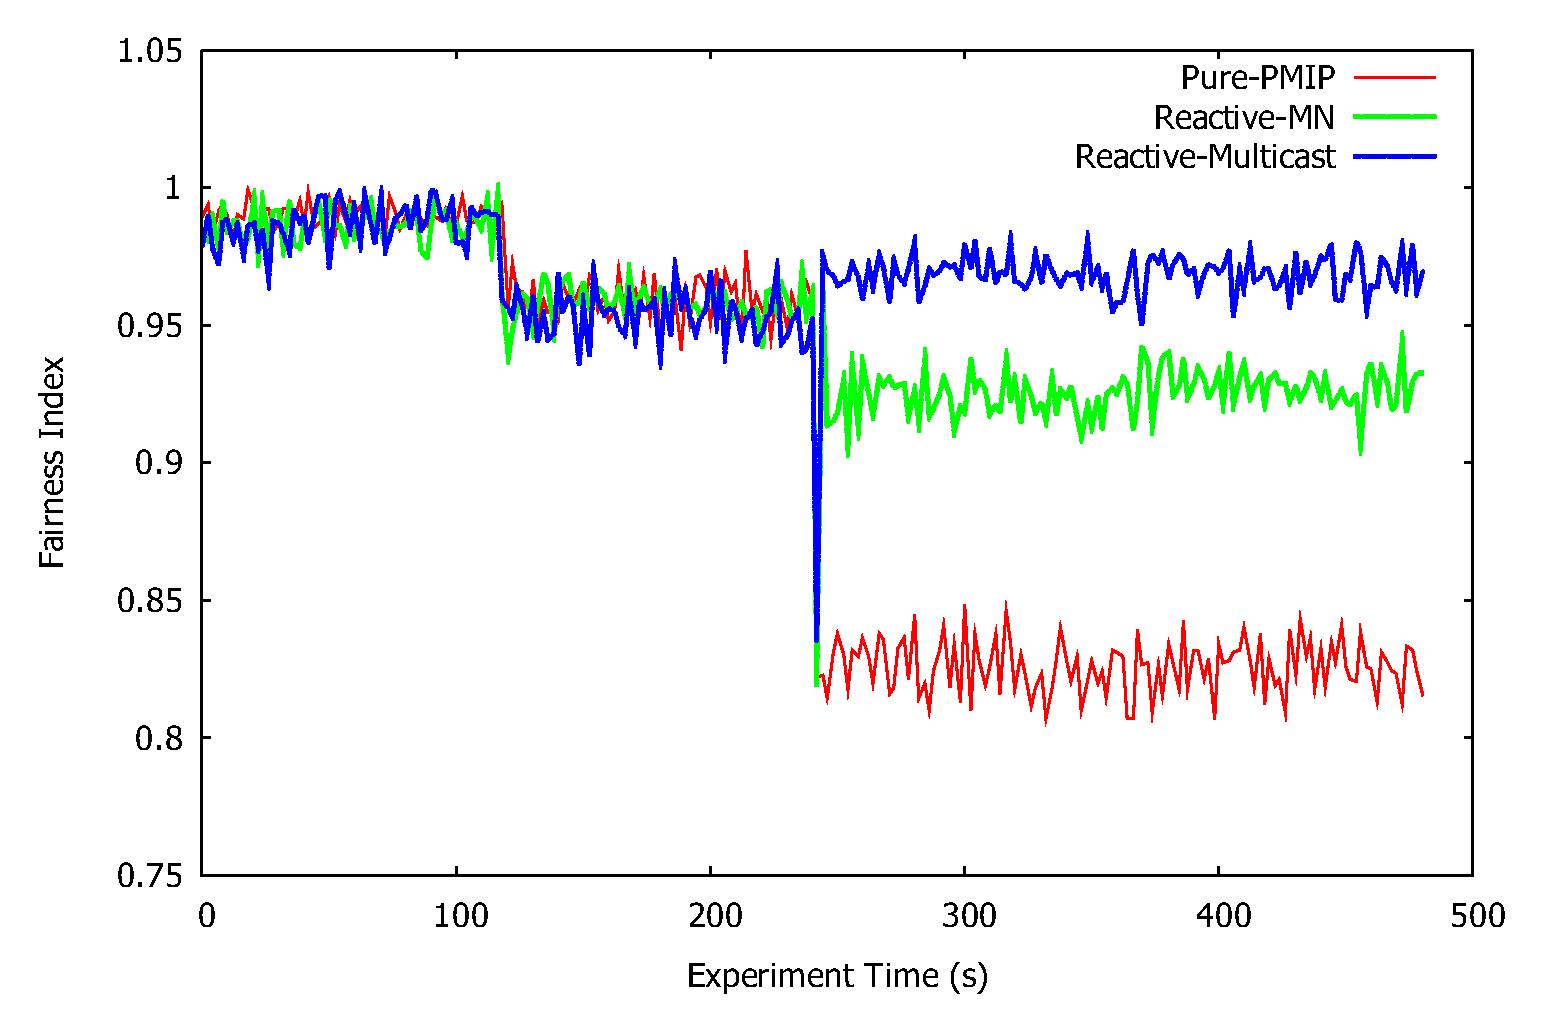
\includegraphics[width=0.47\textwidth]{./Part2/Chapter5/figures/fi_reactive.eps}\label{fig:fi_reactive}}
\caption[Fairness Index for the multicast-based load balancing mechanisms.]{FI value in the experiment 2: (a) Scenario 1, (b) Scenario 2.}
\label{fig:scenario1}
\end{figure}

Fig.~\ref{fig:fi_reactive} plots the FI value in the scenario 2. At the beginning (from 0 to 120 ms), when each LMA has to serve three identical channels, the LMAs' load is nearly equal. As a result, the FI value in three approaches is almost the same and very close to 1. 
As the data rate of the existing multicast flow in $LMA_{1}$ is increased ($C_{11}$'s data rate is increased from 400 Kbps to 800 Kbps), $LMA_{1}$ load is increased accordingly. Meanwhile, the load of $LMA_{2}$ and $LMA_{3}$ is decreased (channel $C_{21}$ at $LMA_{2}$ and $C_{31}$ at $LMA_{3}$ are terminated). Consequently, the FI value is decreased. Since the reactive LB mechanism is only evolved when the LMA load exceeds the threshold value (85\%), the FI values in three approaches are kept the same when the LMAs are running under a heavy load. When $LMA_{1}$ is overloaded (at about 240s, as $C_{22}$'s data rate is increased from 400 Kbps to 1.2 Mbps), the LB mechanism is involved. As a result, the FI value in the reactive-MN and reactive-multicast is clearly greater than that in the pure-PMIP environment. That means the load is better shared between the LMAs. Moreover, the reactive-multicast approach gives a better performance than the MN-based (FI value is greater). In more details, the multicast channel with the highest data rate ($C_{12}$ with 1.2 Mbps) is moved from $LMA_{1}$ to $LMA_{3}$ in the reactive-multicast approach, while one MN (among two) subscribed to this channel is moved to $LMA_{3}$ in the reactive-MN approach. 
\begin{figure}[h!]
\centering
\subfloat[]{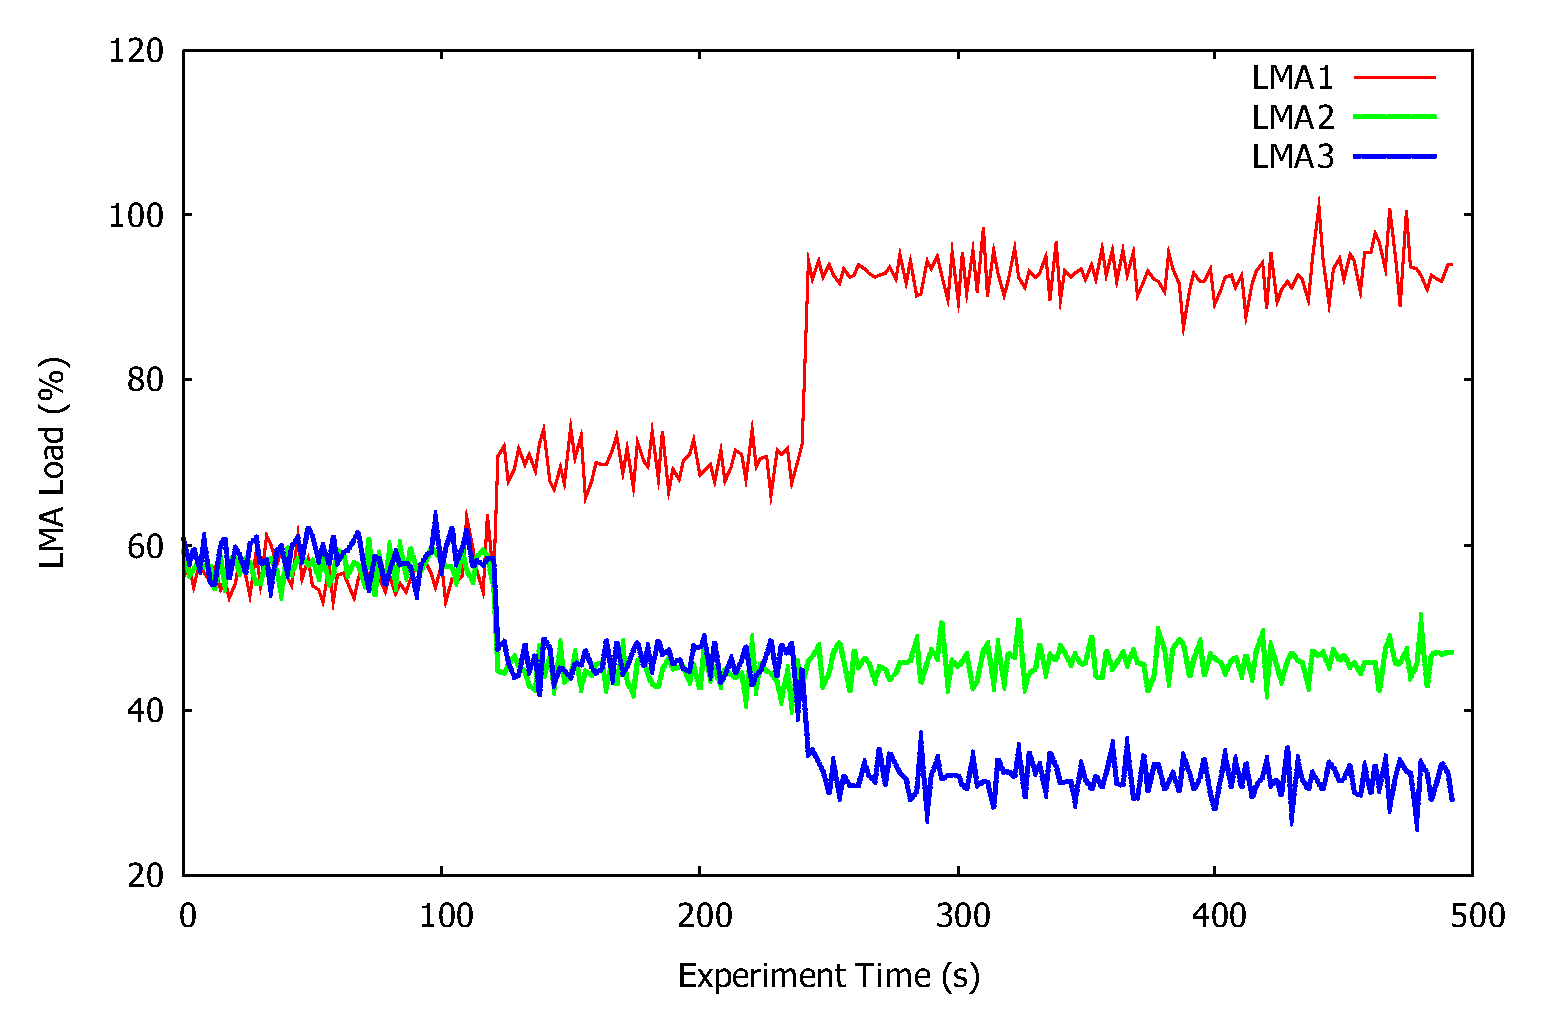
\includegraphics[width=0.35\textwidth]{./Part2/Chapter5/figures/reactive_PMIP_result.eps} \label{fig:s2_pure_pmip}}
\subfloat[]{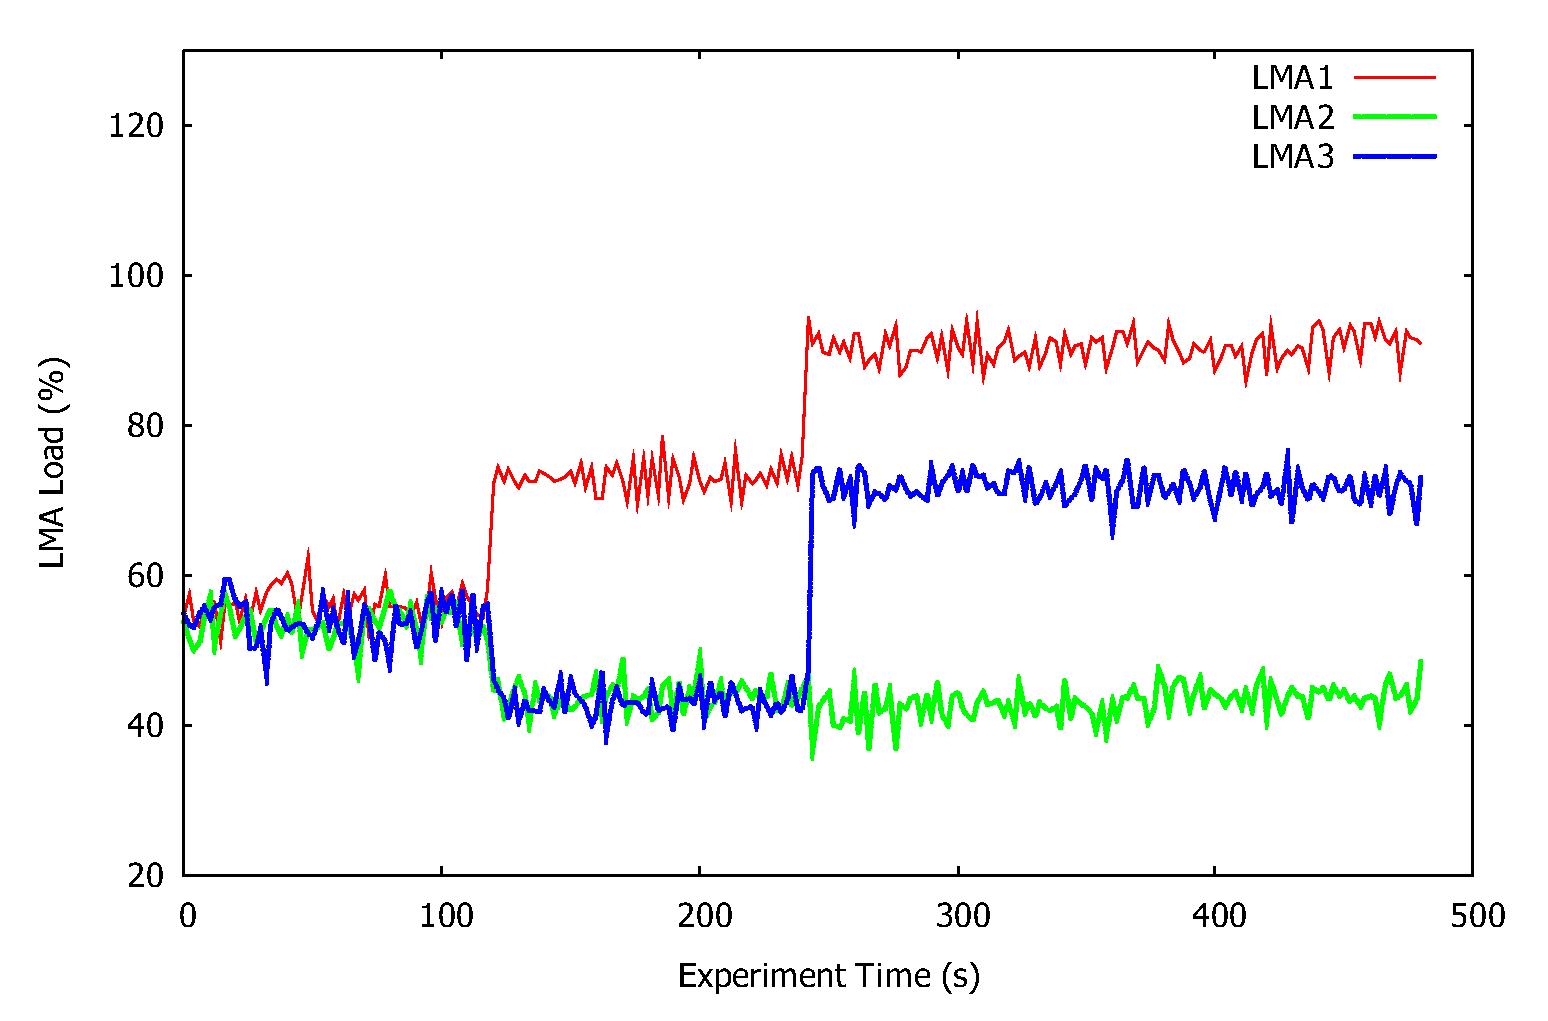
\includegraphics[width=0.35\textwidth]{./Part2/Chapter5/figures/reactive_mn.eps}\label{fig:s2_reactive_mn}}
\subfloat[]{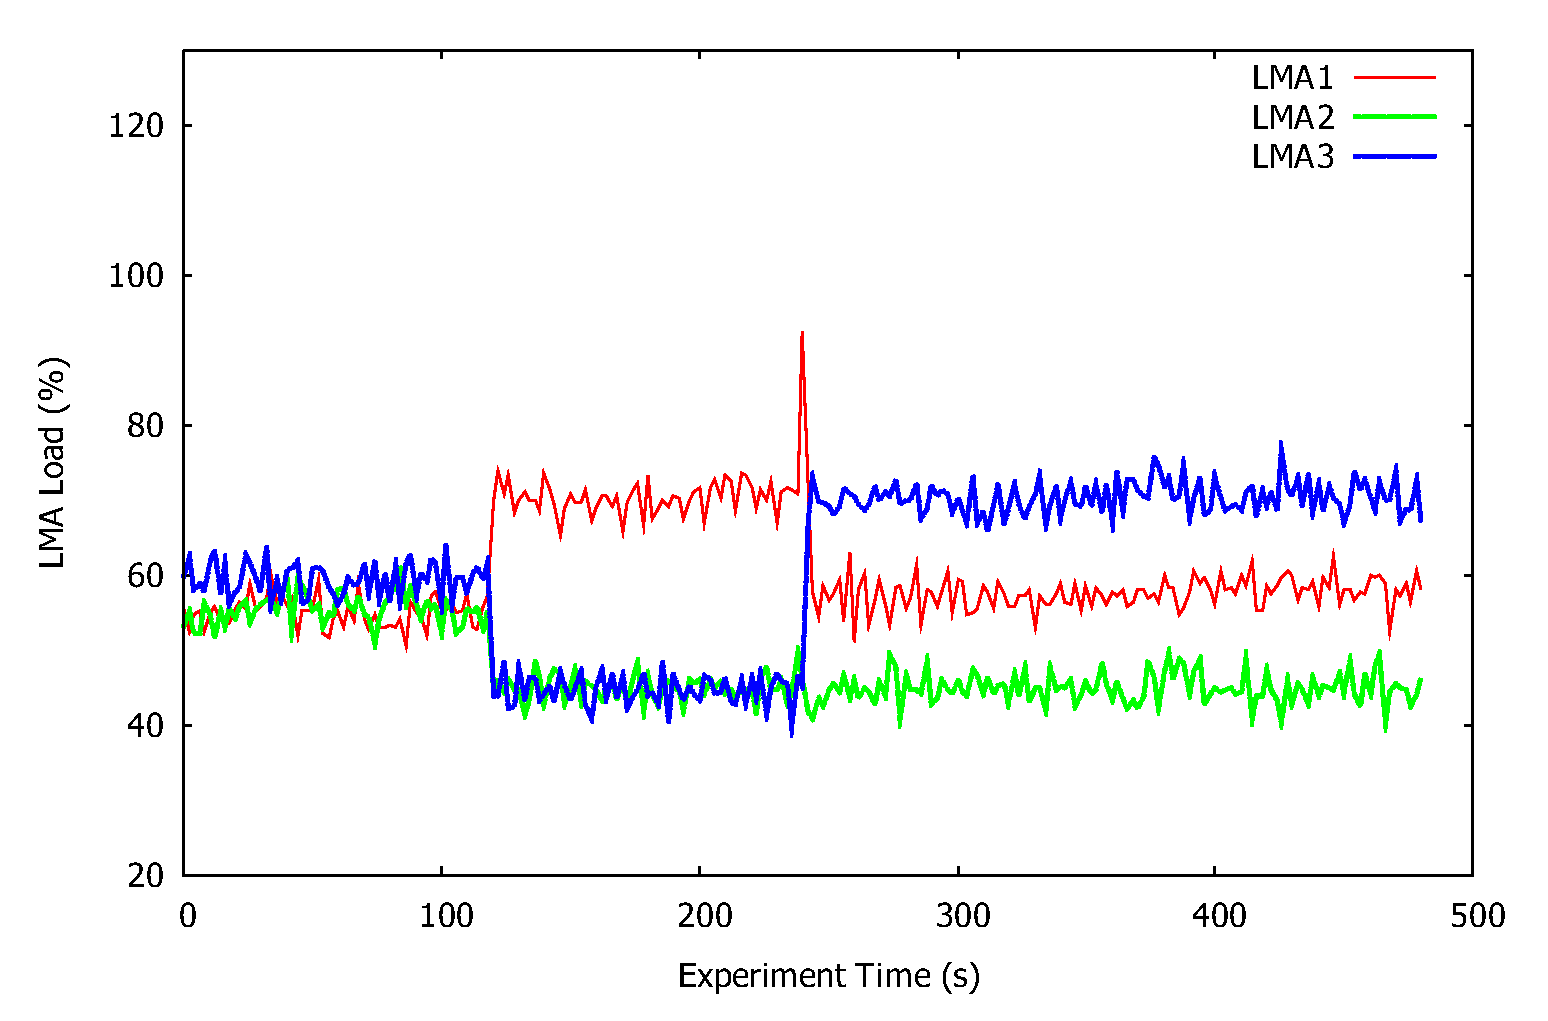
\includegraphics[width=0.35\textwidth]{./Part2/Chapter5/figures/reactive_multicast_result.eps}\label{fig:s2_reactive_multicast}}
\caption[LMA load in the experimentation.]{LMA load in the scenario 2 (experiment 2): (a) pure-PMIP , b) reactive-MN approach, (b) reactive-multicast approach.}
\label{fig:scenario2}
\end{figure}
The detail of load distribution of different approaches is plotted in Fig.~\ref{fig:scenario2}. The reactive-multicast helps avoid $LMA_{1}$ from being overloaded. Meanwhile, the overload status cannot be resolved in the reactive-MN approach ($LMA_{1}$ is still overloaded, while $LMA_{13}$ load is greatly increased). As a result, the total load of all LMAs is significantly increased compared to that in the pure-PMIP and reactive-multicast approach. It is due to the fact that the $LMA_{3}$ has to join the channel $C_{12}$ while $LMA_{1}$ continues forwarding this channel. In this case, more than 31\% of the LMA capacity is wasted. 
\subsection{Multicast Service Disruption Time}
In this subsection, the following parameter values are used: $t_{mm}$ = $t_{ll}$ 
= $t_{la}$ = $t_{rr}$ = 10 ms, $t_{ml}$ = $t_{mc}$ =20 ms, $t_{wl}$=15 ms, $t_{join}$ =13.5 ms, $D_{L2}$ = 50 ms, and $t_{qrd}$ = 374.2 ms. $t_{cv}$ is typically in seconds (for example, the default value in case of OSPF is 10 seconds) \cite{ospf_convergence,ospf_timer}. In this subsection, it is set to 1s. The value of $n_{mr}$ is varied over a range [0, 10] hops. It is noted that most parameters used in this evaluation are set to the typical values found in \cite{Thinh_WCNC_Multicast} and \cite{dsrm}. 

\begin{figure}[h!]
\centering
\subfloat[]{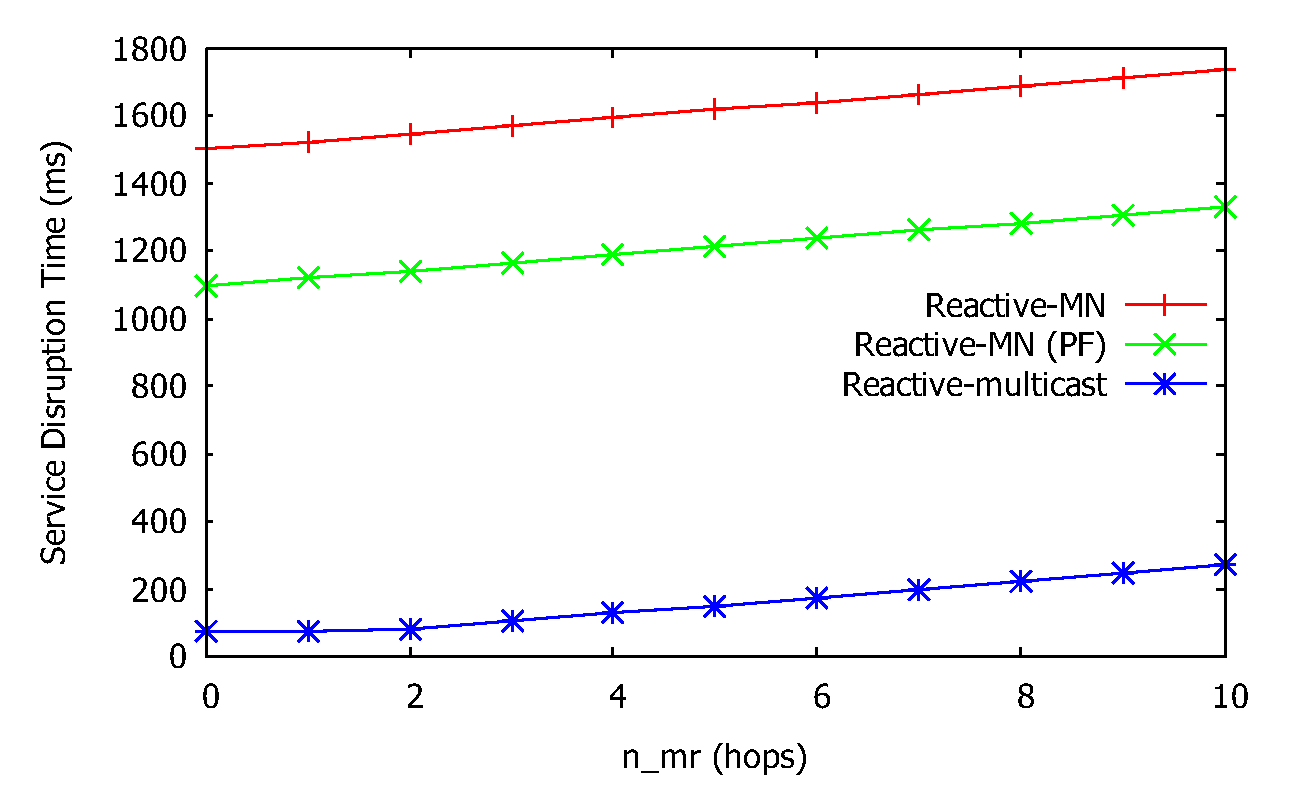
\includegraphics[width=0.47\textwidth]{./Part2/Chapter5/figures/c7_sd_n_mr.eps} \label{fig:service_disruption}}\,\,\,\,\,\,
\subfloat[]{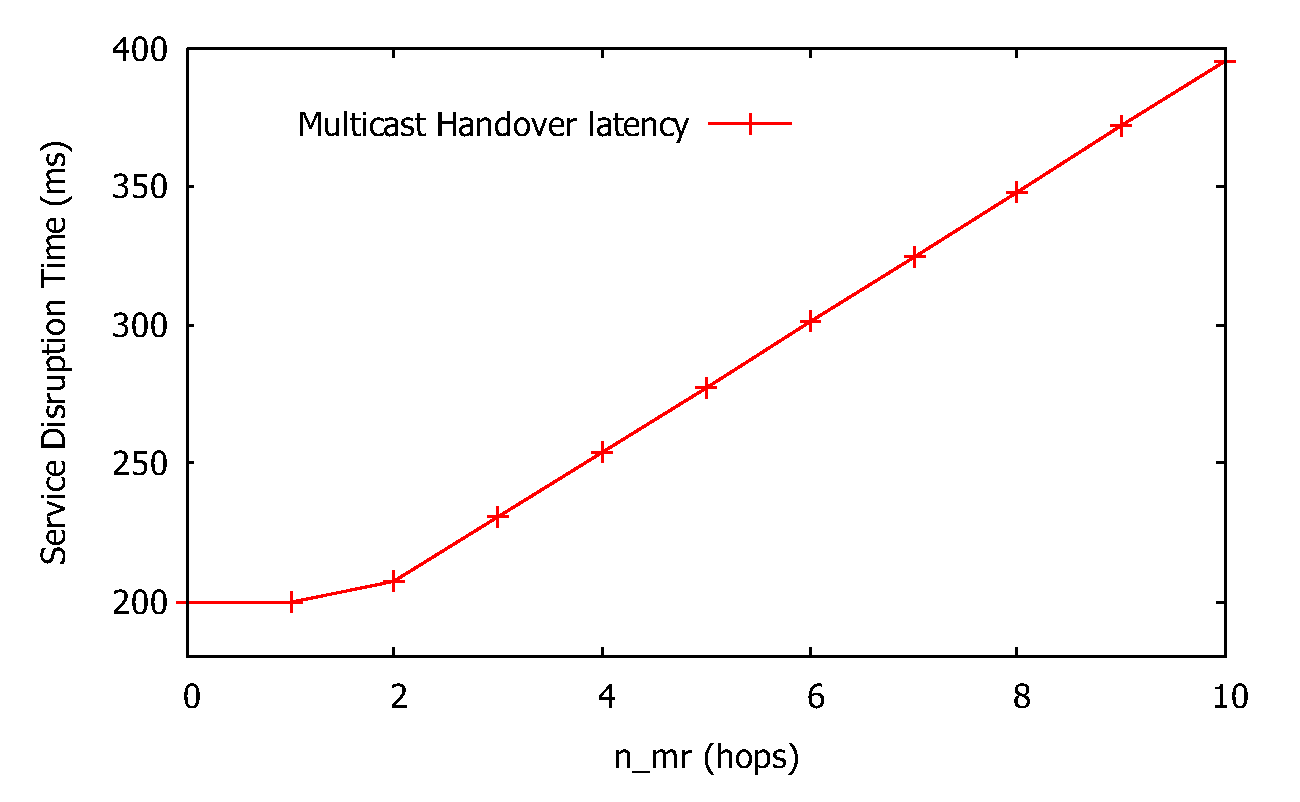
\includegraphics[width=0.47\textwidth]{./Part2/Chapter5/figures/c7_ho.eps}\label{fig:service_disruption_HO}}
\caption[Service disruption time as a function of the average hop-count distances.]{Service disruption time as a function of $n_{mr}$: (a) caused by LB mechanisms, (b) by handover.}
\label{fig:sd}
\end{figure}

Fig.~\ref{fig:service_disruption} shows the multicast service disruption time as a function of $n_{mr}$. It appears clearly that the service disruption in the reactive-MN ($D_{R\_MN}$ and $D_{R\_MN\_PF}$) is definitely higher than the maximum tolerant interruption time for normal services, as specified in \cite{interruption_requirements} is 500ms. Thus, it causes a noticeable service disruption. On the other hand, the service disruption in the reactive-multicast is kept below the value of 300ms, thus, satisfying the requirements for the real-time services. In other words, the reactive-multicast approach helps greatly reduce the service disruption compared to the reactive-MN solution. Moreover, in the reactive-multicast approach, if there exist the LMA which already had the forwarding state for this channel and is not overloaded, it should be chosen as the tLMA. As a result, it is high probably that the $d_{join}$ and $d_{deliver}$ are ignored. That means in most cases $D_{R\_M}$ is 75 ms. 

Fig.~\ref{fig:service_disruption_HO} shows the service disruption time during handover as a function of $n_{mr}$. We could observe that when $n_{mr}<6$, the handover latency is below the value of 300 ms. Moreover, in most cases the multicast traffic is already available at the tLMA, thus, the service disruption during handover is 200 ms. Consequently, the handover impact on the quality of multicast flow is almost imperceptible.
\section{Conclusion} \label{ch7:conclusion}
As the multicast is expected to be widely used in the future networks, degrading the role of the multicast in the available LB mechanism can cause some issues not only from LB perspective (degradation of efficiency) but also from multicast perspective (tunnel convergence problem and service disruption).  To overcome these issues, a multicast-based solution has been proposed. The benefit of the solution is that it does not influence the other ongoing unicast/multicast sessions. It can also co-operate with the existing LB proposals to improve the performance of the network.

Via a near-to-real testbed, the experiment results show that the proposed solution helps better distribute the load imposed by the multicast service among LMAs. Additionally, it helps greatly reduce the multicast service disruption time caused by a changed LMA for LB purpose compared to the existing proposals, even satisfying the service disruption requirement for the real-time services.  

However, from the performance analysis and the experiment result, we conclude that none of the two solutions is complete. The multicast-based solution in general works well in the domain where the mobile data traffic is dominated by the multicast traffic; the unicast-based solution, in contrast, works well with the unicast-dominated domain. For instance, the multicast-based solution may be the most convenient for distributing load among the multicast tree mobility anchors (MTMA) which work as a topological anchor point for the multicast traffic in a PMIPv6 domain \cite{ro_pmip}. It comes from the fact that the MTMA only serves the multicast traffic. As a result, the multicast-based should co-operate with the MN-based solution to enhance the reliability and scalability of  the network. For example, the proactive-MN can be applied when an MN enters the PMIPv6 domain, while the proactive-multicast is evolved when a multicast session is initiated. Besides, the reactive-multicast can be followed by the reactive-MN approach. At this stage, if any multicast session is not a real-time and delay sensitive one, the reactive-multicast approach will be performed. Otherwise, the reactive-MN will be executed. The main idea is that we try to distribute load among LMAs by using the multicast-based solution before applying the reactive-MN solution to avoid the influence on the ongoing sessions. Therefore, the blocking probability of a new MN (session) and the dropping probability of the existing MNs (sessions) are obviously lower than the existing LB mechanisms (lower is better).






\chapter{Mobility in Heterogeneous Networks: Electric Vehicle Charging Service Use-Case} 
\label{ch:EVCS}
In this chapter, the mobility in heterogeneous networks will be illustrated via a use case: Electric Vehicle Charging Service (EVCS). There are several reasons for selecting this use case. Firstly, the electric vehicle (EV) is a promising choice for personal transportation in the near future. Secondly, the idea of connecting vehicles is gaining momentum. In addition, a mobile node, an EV in this context, can be connected with the infrastructure via different wireless/wired technologies in different steps (LTE while driving, WLAN while approaching a charging infrastructure, PLC while being docked at a charging infrastructure). Thus, considering multicast in the EV is one step to enable the entertainment system in the EV, which is becoming more and more popular. Moreover, IP multicast can also be used to update the software of the in-vehicle systems.

According to Cisco Internet Business Solutions Group (IBSG) \cite{IBSG_connected_vehicle}, connecting vehicles creates such significant benefits as traffic safety, environmental eco-friendly, easing traffic congestion, and enhancing driver/passenger experience (in-vehicle infotainment systems). Four key capabilities in the connected vehicle are connection within the car, connection to personal devices, connection \textit{around} the car and connection to the cloud (or infrastructure). These capabilities make a vehicle as a \textit{personal digital assistant on wheels} \cite{IBSG_connected_vehicle2} keeping peoples connected to the Internet of Things. Thus, they make our travel experience safer and more convenient as well as enhance the in-vehicle experience \cite{IBSG_connected_vehicle2}. In line with this trend, the EVCS gains the benefits of connecting vehicles to provide a smart charging service from both user and electricity operator perspective. 

\section{Introduction}
The number of vehicles in use is set to increase exponentially in recent years (1.015 billion in 2010 \cite{vehicle_population}). This trend causes some serious issues regarding energy sources like increasing in fuel demand and costs \cite{evci_mit}, environmental concerns \cite{gas_emission} and air quality. On one hand, it encourages the production and use of clean and efficient energy vehicles in which the electric vehicles (including full electric and plug-in hybrid electric vehicles, in common, EVs) belong to. On the other hand, the evolution of battery technology allows increasing the battery capacity while decreasing the weight/size of battery pack and reducing the costs. This context makes the EV a promising choice particularly for individual mobility in the cities.

In order to gain the customer acceptance of the EV, the charging infrastructure needs to be deployed at least as numerous and widespread as the fueling stations. Yet, unlike the fueling station, the various available charging strategies requires unprecedented interactions between drivers and the Grid operators. Secondly, the type of charging stations will range from the commercial stations to the single plugs operated in parking lots or in residential areas. Altogether, this will lead to a segmentation of Electric Vehicle Charging Services (EVCS), with a complex tracing of charging contexts and payment, which would make the charging process difficult and charging capacity/need unforecastable for Grid operators, adding anxiety to users and Grid operators. One solution to mitigate such situation is to make heterogeneous charging strategies and stations, as well as  and the natural mobility of EVs transparent to the EVCS. 

As stated in \cite{EV_smart_grid}, the critical requirement to get energical and economical benefits from Smart-grid and EVs is to reach an optimal scheduling of charging EVs and storing electricity by EV. 
Uncoordinated burst of EV charging may cause a huge energy demand that can result in the electrical grid congestion, while storing electricity by EVs may be inefficient if required immediately elsewhere. Thus, it is important for Grid operators to monitor the necessary data (like energy consumption and demand) and to assign and route vehicles to the appropriate charging stations supporting their required charging policies. Such negotiation cannot be conducted at the charging station but must be conducted while driving. The EV therefore needs to communicate with the charging infrastructure \cite{plc_smart_grid}. In this context, several access technologies (e.g., WLAN, LTE and Power Line Communication (PLC) \cite{wireless_plc}\cite{plc_full}) must be used at different phases of the EVCS, such as LTE while driving, WLAN while approaching a charging station, and PLC while being docked at a charging station. Such heterogeneous communication technologies should be transparent to the user, the Grid operator and to the EVCS in order to maintain the service context. 

In this chapter, we propose an EVCS solution from both user and Grid operator point of view. For the user, it provides a ubiquitous and transparent charging service at different scenarios (at home, at a charging station and at a parking), making charging an EV as simple as possible. It also helps the Grid operator to efficiently manage the user consumption/demand to control the load on the grid especially when a large number of EVs is considered. From the centralized nature of Smart-grid services, a network-based IP mobility management solution, Proxy Mobile IPv6 (PMIPv6) \cite{PMIPv6}, is most appropriate to federate segmented charging services and make the charging experience transparent to EVs mobility as well as the communication technology used by each phase of the EVCS. By using PMIPv6, the service takes care of the EV mobility, handling vertical and horizontal handovers between different communication technologies (e.g., WLAN, LTE and PLC). Yet, IPv6 address preservation in PMIPv6 remains an issue in such context, and we provide a solution by relying on a logical interface approach to hide the change of interface to the IPv6 stack. Finally, we will validate the EVCS concept and the performance of PMIPv6 for the EVCS against benchmark from IEEE 1646. The mobile multicast in heterogeneous networks is also taken into consideration. A near-to-real testbed, which is a combination of real and virtual machines, has been deployed to reduce the hardware cost and to provide more flexible experiment. A real PLC connection provided by partners from the VELCRI project is used to obtain realistic results.\\ 

In the context of this thesis, this chapter discusses the mobility of the nodes in heterogeneous networks, mainly from a mobile node point of view. In other words, the MN will move in a PMIPv6 domain using different access technologies e.g., WLAN, LTE and PLC. Thus, both vertical and horizontal handover will be considered. A vertical handover is executed when the mobile node changes the type of technology it uses to access the network, while a horizontal handover is performed between two layer 3 point of attachment using the same technology. Also, IP multicast will be taken into account. From a mobile node point of view, to obtain the same IPv6 address when switching between different interfaces, logical interface mechanism is used. Moreover, it helps to hide the changing of the interfaces from multicast application point of view. Also, the IEEE, through its 802.21 work group\footnote{IEEE 802.21 Working Group, http://www.ieee802.org/21/index.html}, has developed a standard that allows a MN to seamlessly roam across different types of 802 network access technologies e.g., WLAN, WiMAX and LTE. The solution based on the Media Independent Handover (MIH) Services has been deployed in the Medieval project \cite{d4.1}. Thus, we do not mention MIH-based solution in this chapter. 

The structure of this chapter is as follows. Section \ref{ch8:evcs} describes a solution for EVCS regarding different charging use cases, design principles, and operations. Section \ref{ch8:pmip} briefly introduces PMIPv6 in the context of EVCS and considers multicast in the context of EVCS and heterogeneous networks. While section \ref{ch8:experimentation} describes the testbed, experiment scenarios and the experiment results. Finally, conclusions are presented in the last section.

\section{Electric Vehicle Charging Service} \label{ch8:evcs}
In this section, starting from the deployment scenarios for EVCS, the usage scenarios, the design principles as well as the operations of the EVCS are briefly provided. Further discussions on EVCS can be found in \cite{PMIP_EV,velcri_report}. This section also makes an early highlight on the reasons why PMIPv6 is a good choice in the context of EVCS.

\subsection{Electric Vehicle Charging Deployment}
In the context of VELCRI project, there are three types of charging strategies, namely standard, rapid and ultra-rapid. The standard charge may take from 4 to 8 hours to provide a full charge upon the initial state of battery, while the rapid and the ultra-rapid charge need about 30 minutes and 5 minutes, respectively. The location of the charging pods may vary, however, three typical places with the corresponding characteristics are considered:
\begin{itemize}
\itemsep 0.1em
\item Charge at home: long charging time at low power;
\item Charge at a station: short charging time related to average fueling time; requires a high peak power level, which limits the simultaneously charging pods at stations;
\item Charge at a parking: charging time related to the time spent in the parking, reduced peak power but large amount of charging pods, which requires flexible charge scheduling.
\end{itemize} 

From the characteristics of different types of charge and locations, Table.~\ref{tap:type_location} shows the possible deployment scenarios of charging system. It is worth noting that the scenarios marked $\textit{possible}$ are not considered in this chapter.

\begin{table}[ht]
\footnotesize
\captionsetup{font=footnotesize}
\caption[Electrical vehicle charging system deployment: type and location.]{Charging System Deployment: Type and Location}
\label{tap:type_location}
\centering
\begin{tabular}{|c |c |c |c |}%{|l|l|l|l|l|l|}%
\hline
\textbf{Charge Type $\backslash$ Location} & \textbf{Home} & \textbf{Station} & \textbf{Parking}   \\
\hline
\textbf{Standard charge} &  $\surd$ & - & (possible)\\
\hline
\textbf{Rapid charge}  & - &  (possible)  & $\surd$ \\
\hline
\textbf{Ultra-rapid charge} & - & $\surd$&  (possible)  \\
\hline
\end{tabular}
\end{table}

\subsection{General Use Cases for Electric Vehicle Charging Service}
\begin{figure}[h!] 
 \begin{center} 
 \includegraphics[width=0.75\textwidth]{./Part2/Chapter6/figures/c8_use_cases.eps}
    \caption[General use cases of the electrical vehicle charging service]{General use cases of EVCS.}
     \label{fig:c8_use-cases}
  \end{center} 
\end{figure}

Based on the charging deployment scenario, four general use cases for the EVCS are considered (see Fig.~\ref{fig:c8_use-cases}): (a) charging at home, (b) charging at a station, (c) charging at a parking, and (d) moving between the stations/parkings. 
\paragraph{Charging at Home} The network at home can be considered as home network of the EV. The EV is typically charged in the evening (period of high energy demands and high cost) when the EV owners return home. Thus, the EV needs to be charged intelligently. It can be done thanks to the intelligent charging management which is responsible for the automatic charge/discharge of the EV in order to lower cost and effectively control/optimize the load on the grid.
\paragraph{Charging at a Station} The EV, at first, communicates with the infrastructures via the wireless access technologies e.g., WLAN and LTE to assign and route vehicles to the appropriate stations. At the station, the EV will be plugged into an electrical outlet (using PLC connection) to charge. A vertical handover between WLAN/LTE and PLC will be performed that allows the EV to continue communicating with the charging station. Again, the charging process will be taken care by the intelligent charging management. The EV can also use additional services during the charging process. After the charging is done, the EV may receive a bill including the charging-related information (time and cost), the EV profile and operator's information.  
\paragraph{Charging at a Parking} The steps prior to parking are similar to those in the previous case (charging at a station). The charging schedule can also be negotiated. Because of the difference between station and parking, localized service can be provided to route vehicles to the appropriate charger. 
\paragraph{Moving between the Parkings}
In some cases, the charging process is interrupted. The context related to this EV will be stored at a database. After connecting to another parking, the EV can make an attempt to keep the same negotiation or fall back to a renegotiation in case the parking fails to support the requirements. In the first case, the context will be restored (preservation of the context) at the current parking.
\subsection{Design Principles}
To deal with different usage scenarios of EVCS, we proposed a solution guided by a set of design
principles as follows:
\begin{itemize}
\itemsep 0.07em
%\vspace{-0.07in}
\item Transparency: transparent mobility of the user to the service. It allows EVs to use the charging system as similar as at home (e.g., context preservation and under only one contract);
\item Pre-negotiation: negotiation with the charging infrastructure before deciding to go to a specific station/parking to charge (pre-negotiation);
\item (Intelligent) Charging management: cost minimizing (for user) while maximizing system reliability and stability (for Grid operator);
\end{itemize}

Moreover, the EVCS should provide an easy-to-use service and secured transactions (from user perspective), as well as an effective way to manage the user information (energy demand, consumption, and location) to better control the load on the grid (from Grid operator perspective).

Therefore, the charging service can be divided into the basic modules which are mapped to the design principles as described in Fig.~\ref{fig:modules}.
\begin{figure}[h!] 
 \begin{center} 
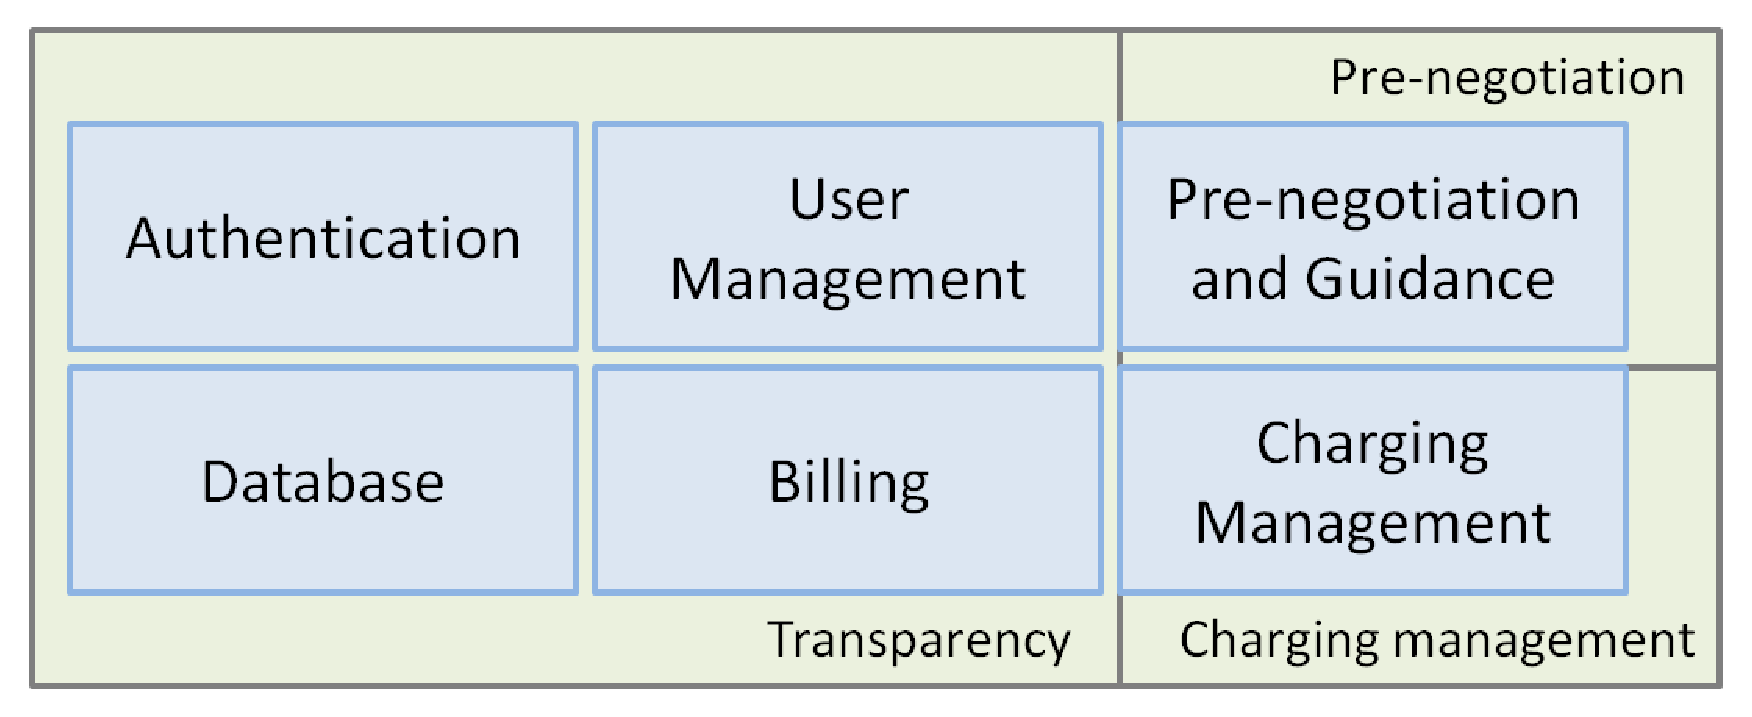
\includegraphics[width=0.6\textwidth]{./Part2/Chapter6/figures/modules.eps} 
   \caption[The EVCS's modules.]{EVCS modules reflect the design principles.}
   \label{fig:modules}
 \end{center} 
\end{figure} 
\subsection{EVCS: Operations and Functionalities}
Following its design principles, the EVCS is proposed with the main operations as briefly described as follows (further information can be found at \cite{velcri_report}):
\paragraph{Session initiation (via WLAN/LTE/PLC)} It is executed when an EV is connected to the charging infrastructure for authenticating/authorizing and obtaining the EV profile (context establishment). PLC is used for the session initiation only in case of charging at home. 
\paragraph{Session negotiation and guidance (via WLAN/LTE)} This operation allows the EV to negotiate with one or multiple charging infrastructures to find the most appropriate one based on such metrics as charging time, cost (for user), charging type, required capacity and slots availability (for Grid operator). It is noted that this step is executed before reaching a charging station/parking thanks to the wireless access technology (WLAN/LTE). Also, additional information of the station/parking can be provided like discounts and bonuses.
\paragraph{Charging management (via PLC)} Charging process does not start as soon as the EV is plugged, but is rather scheduled according to the capacity of the grid and the demand of the user established during the negotiation phase. Accordingly, an intelligent charging management unit coordinates the charging process on bi-directional communication link between the infrastructure and the EV while being plugged. In other words, the EV can be charged when the demand is low, otherwise it can be considered as a distributed energy source when the demand is high.  
\paragraph{Session termination (Billing, via WLAN/LTE/PLC)} When a session is terminated, electricity used or sold as well as related statistics (price, charging time and charging type, etc.) will be logged to the service provider and the cost charged on the user account as if the user was at home. 

\section{PMIPv6 for Electric Vehicle Charging Service} \label{ch8:pmip}
In the context of EVCS, since an EV can be charged at different places as similar as at home, PMIPv6 is a good choice. It is because it makes heterogeneous communication technologies transparent to the EVCS and hides the mobility of the EVs to the service. 

As we can see in Fig.~\ref{fig:c8_use-cases}, using PMIPv6 offers some benefits in the context of EVCS: (1) Network-based mobility management and Address preservation: The MAG where the EV is currently connected simulates the EV's home network. Therefore, the EV uses the same IPv6 address when moving in a PMIPv6 domain. So, the EV is not aware of the mobility; (2) Context preservation: This feature facilitates the charging process of the EV in case of mobility; (3) Location management; (4) Easy-to-integrate with Authentication, Authorization and Accounting (AAA) mechanism; and (5) EV-Grid interaction: The PMIP messages can be extended for collecting the EV-related information. Thanks to the advantages of PMIPv6, the energy and utility suppliers can provide an easy way but flexible to access their services. 

Although PMIPv6 can bring benefits to the EVCS, it has several limitations. Thus, improvements are needed to make PMIPv6 suitable for the EVCS.
\paragraph{Handover across heterogeneous access technologies (WLAN, LTE and PLC) - IPv6 Address Preservation} Considering handover across different access technologies (vertical handover), there are several mechanisms which allow the EV to obtain the same IPv6 address after handover. The first one is based on the auto-configuration mechanism by using a common identification for both PLC and WLAN interface (like Network Access Identifier). The second one uses the Dynamic Host Configuration Protocol (DHCP) mechanism in which two interfaces must be set with the same client identifier. However, the major limitation of these two approaches is that two interfaces cannot be active at the same time. As the result, it may cause a significant service disruption and packet loss. 
    
The third mechanism uses the logical interface technique \cite{logical_inteface} which allows to hide the different access technologies (e.g., using Linux bridge mechanism). Thus, the changing of interface is transparent to the IP stack. Moreover, two interfaces can be active at the same time. For this reason, this mechanism is more suitable than the others to facilitate the vertical handover in terms of handover latency. Note that in the context of electric vehicle, with a huge power, the impact of power consumption caused by turning on both of the interfaces is negligible. 
\paragraph{Context Preservation} To support the context preservation characteristic, the MN's context needs to be stored in a database/policy profile. One possible solution is that the AAA server is extended to store this type of information. 

\subsection{Multicast Considerations}
\begin{figure}[h!] 
  \begin{center} 
    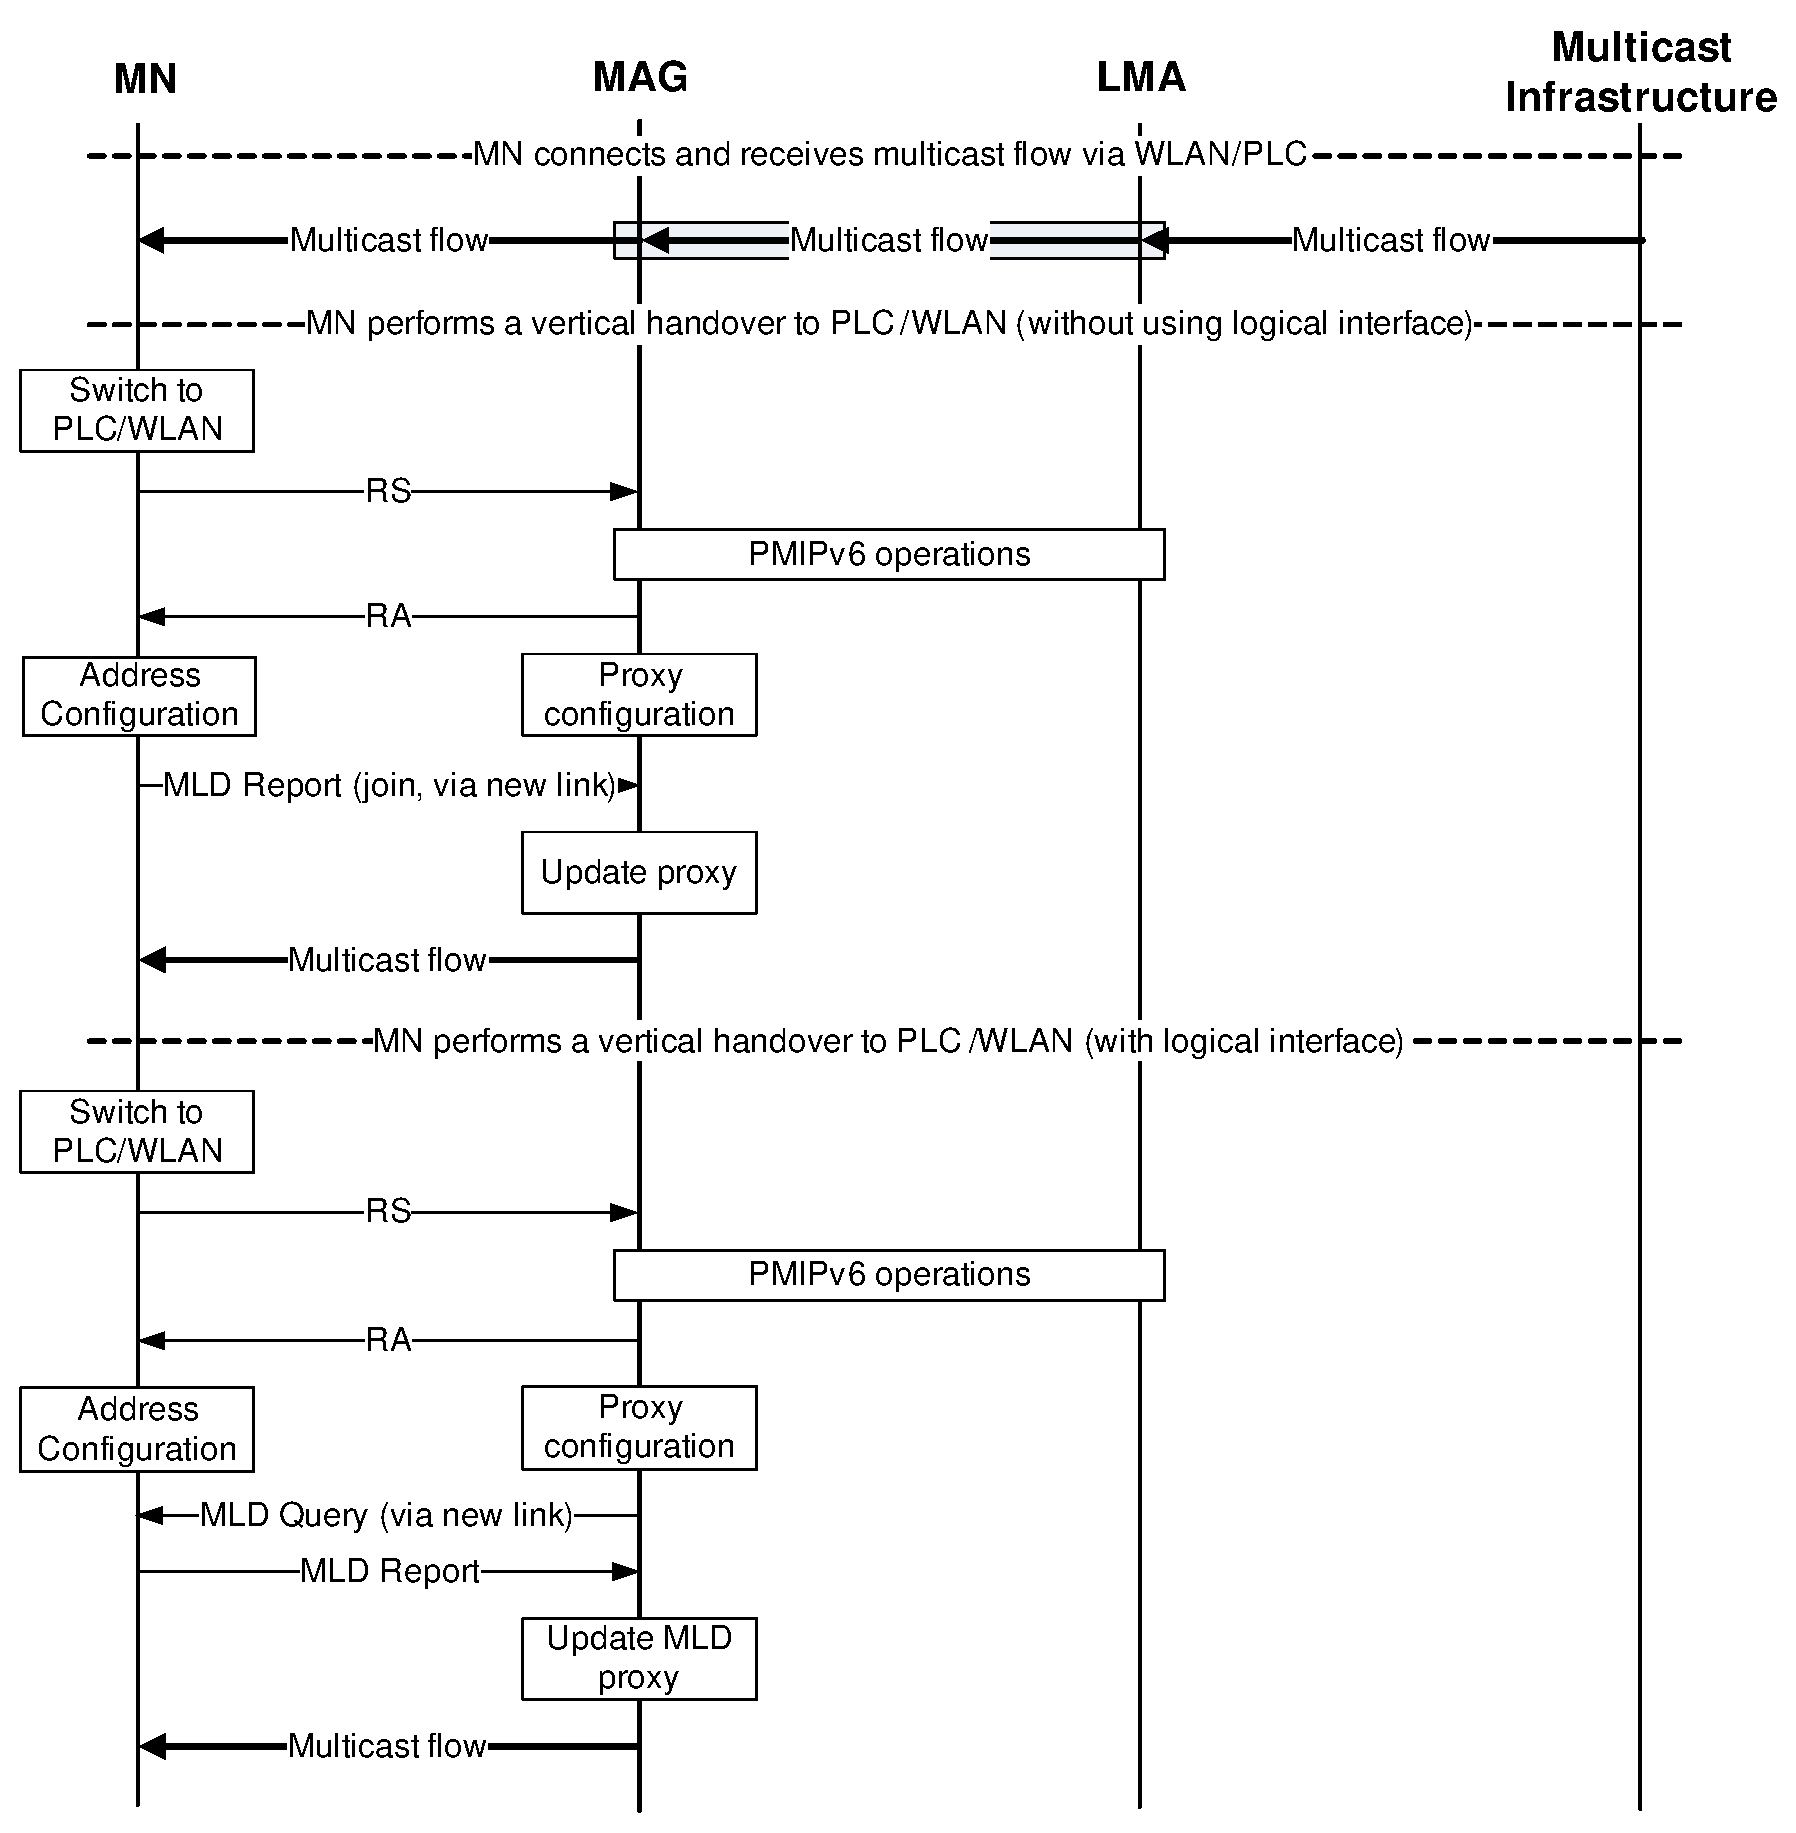
\includegraphics[width=0.80\textwidth]{./Part2/Chapter6/figures/c8_handover_base.eps} 
    \caption[The multicast-related signaling when an EV changes its point of attachment.]{Handover signaling regarding multicast.}
    \label{fig:c8_handover_base}
  \end{center} 
\end{figure}
When an MN (a listener) performs a vertical handover between two interfaces while connecting to the same MAG, the normal PMIPv6 will be executed to allocate a HNP for the new interface. Depending on the PMIPv6 implementation, the MN can obtain the same HNP as for the previous interface or a new HNP. It then configures its IPv6 address based on the prefix allocated. As a normal proxy operation, the MLD proxy at MAG will add the MN to a downstream interface. Moreover, from a listener point of view, the listener should join the on-going multicast flows at the new interface. Thus, the requirement in terms of mobility transparency cannot be guaranteed. Thanks to the logical interface mechanism, the listener does not need to re-join the on-going flows, since the logical interface has already joined them. As a result, the listener is unaware of mobility from the multicast service point of view (see Fig.~\ref{fig:c8_handover_base}). However, even with logical interface, if the on-going flows are not present at this downstream interface, the MN has to wait to receive an MLD Query message to express its active multicast flows by mean of MLD Current State. As stated in the previous section, it may experience a noticeable service disruption (see Fig.~\ref{fig:c8_handover_base}). Thus, the MAG will inform the MLD proxy so that the proxy can update its membership state to forward the on-going multicast flows in the new downstream interface as soon as possible. It can be considered as an extension to MLD proxy. In case of a vertical handover between two different MAGs, the context transfer is needed to reduce the service disruption time as discussed in Chapter \ref{ch:multicast_PMIP}. Again, by applying the logical interface mechanism, the mobility is transparent to the listener.  

When the MN performs a horizontal handover between two MAGs, similarly, the context transfer between these MAGs is required in order to avoid a large service disruption and packet loss. Further information on the handover signaling and operation can be found in Chapter \ref{ch:multicast_PMIP}.
 
\section{Experimentation} \label{ch8:experimentation}
\subsection{Experimentation Setup and Scenarios Description}
In order to validate the proposed solution, a near-to-real testbed has been deployed. In this section, the testbed and the experiment scenarios are presented.
\begin{figure}[h!]
\centering
\subfloat[]{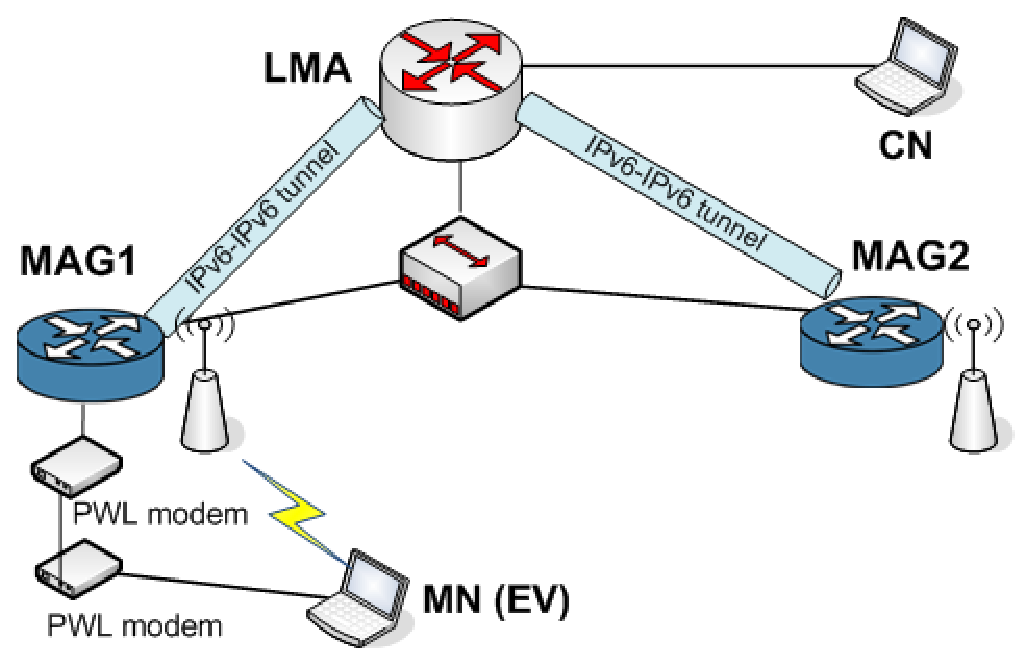
\includegraphics[width=0.47\textwidth]{./Part2/Chapter6/figures/c8_testbed.eps} \label{fig:c8_test-bed}}\,\,\,\,\,\,
\subfloat[]{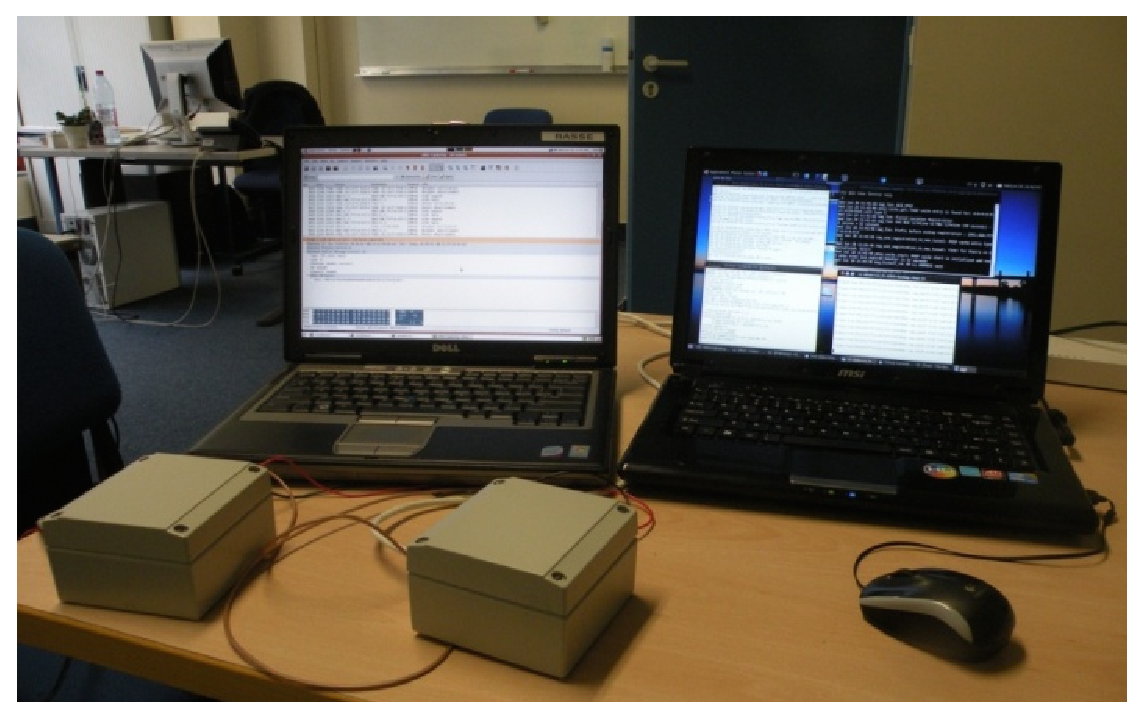
\includegraphics[width=0.47\textwidth]{./Part2/Chapter6/figures/c8_testbed_2.eps}\label{fig:c8_test-bed_2}}
\caption[Testbed implementation for the ECVS experimentation.]{Testbed: a) architecture; b) actual image.}
\label{fig:c8_testbed}
\end{figure}

\paragraph{Description of the Testbed}
The testbed, as indicated in Fig.~\ref{fig:c8_test-bed}, is composed of one LMA, two MAGs, one CN and one MN playing the role of an EV. It is noted that the CN represents an entity in the Smart Grid. The testbed is based on the User-mode Linux (UML) to create the virtual machines. The LMA, the MAGs and the CN are the virtual machines (UML) running on a host machine. Another real machine is used as an EV that connects with the MAG via a WLAN or a PLC connection. To connect the virtual machines, the virtual Ethernet connection is simulated by using a combination of Linux Bridge and TAP interface (for more details, see Chapter \ref{ch:performance_evaluation}). In case of PLC connection, two PLC modems are connected via coaxial cable and to the MN and to the MAG, respectively. Thanks to VELCRI project, a real PLC connection is used in the testbed. The PMIP functionality and multicast support can be deployed similar to in the Chapter \ref{ch:multicast_PMIP}. The actual image of the testbed is described in Fig.~\ref{fig:c8_test-bed_2}. In addition, the mapping between the actual image and the logical components of the testbed is illustrated in Fig.~\ref{fig:c8_mapping}.
\begin{figure}[h!] 
  \begin{center} 
    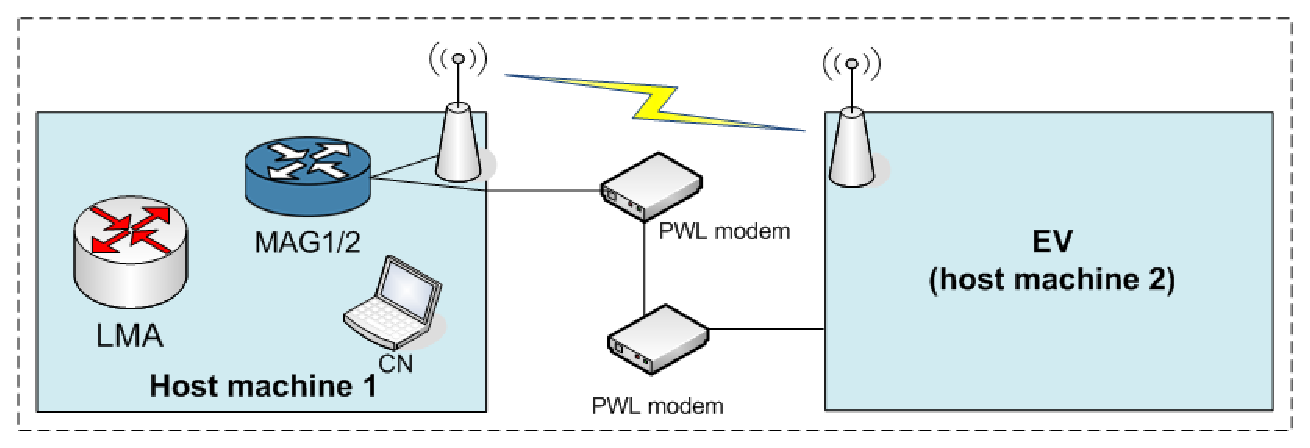
\includegraphics[width=0.65\textwidth]{./Part2/Chapter6/figures/c8_mapping.eps} 
    \caption[Mapping between the actual image and the testbed components.]{Mapping between the actual image and the testbed components.}
    \label{fig:c8_mapping}
  \end{center} 
\end{figure}

During the experiments, a network analyzer tool (e.g., Wireshark) is used to capture the packets exchanged between the entities while a network testing tool (like Iperf) to measure the throughput of WLAN/PLC connection. The Ping application plays the role of a simple service running on EV and CN. When considering multicast, the CN also plays the role of a multicast source broadcasting a multicast flow which is subscribed by the EV (playing the role of a listener).
%\vspace{-0.29in}
\paragraph{Logical Interface Mechanism in Linux}
Logical interface mechanism is applied on the MN using the bridge-utils (bridging)\footnote{Linux Bridge: http://www.linuxfoundation.org/collaborate/workgroups/networking/bridge} and TUN/TAP device for Linux systems as specified in Fig.~\ref{fig:c8_logical_interface}. The TAP device works at the Ethernet frame level while the TUN device acts as a network layer device. We then use the \textit{ebtables} tool\footnote{ebtables – Linux Ethernet bridge firewalling: http://ebtables.sourceforge.net}(or \textit{iptables}\footnote{iptables: http://ipset.netfilter.org/iptables.man.html}), which is a filtering tool for a Linux-based bridging firewall, to switch between the interfaces. 

\begin{figure}[h!] 
  \begin{center} 
    \includegraphics[width=0.4\textwidth]{./Part2/Chapter6/figures/c8_logical_interface.eps} 
    \caption{Logical interface mechanism under Linux.}
    \label{fig:c8_logical_interface}
  \end{center} 
\end{figure}

\paragraph{Experiment Scenarios}
We define four experiment scenarios based on the use cases given in the previous section as follows:
\begin{itemize}
\itemsep 0.07em
\item Scenario 1: Authentication and context establishment. This scenario aims at demonstrating that PMIPv6 can work correctly with PLC.
\item Scenario 2: Vertical handover between WLAN and PLC at one MAG. This scenario describes the transition between the negotiation, the charging management and the termination step. 
\item Scenario 3: (Horizontal) Handover/roaming between two MAGs. From the EVCS point of view, this scenario represents the mobility of the EV between the parkings. It is noted that the horizontal handover in some cases can be replaced by successive vertical/horizontal handovers. Without loss of generality, only a horizontal handover using WLAN is considered.         
\item Scenario 4: Multicast considerations in the scenario 2 and 3. In this case, the CN plays the role of a multicast source broadcasting a multicast flow while the EV plays the role of a multicast listener. Further information about how to generate the multicast traffic in this testbed can be found in Chapter \ref{ch:LB}. In case of handover between two MAGs, the multicast context transfer and the explicit tracking functions are enabled at MAG to reduce the service disruption time as similar in Chapter \ref{ch:multicast_PMIP}.
\end{itemize}

\subsection{Experiment Results and Discussions}
At this step, the experiment focuses on the validation of the concept of EVCS, the performance of PMIPv6 for the future EVCS as well as multicast mobility with heterogeneous communication technologies e.g., WLAN, LTE and PLC. Thus, two evaluation metrics are concentrated, i.e., PMIP functionality and performance metrics which are translated into the corresponding EVCS ones. The first metric aims at validating the functionality of the EVCS regarding the authentication, the context establishment, the address preservation and the service continuity in case of handover. The second metric takes into account the response time (Round-Trip Time (RTT) between the EV and the CN), handover latency, throughput and packet loss in case of unicast traffic; while handover latency, packet loss in case of multicast traffic. From the EVCS point of view, the response time is the time needed for exchanging information between EV and charging infrastructure (stations and Smart Grid) for controlling and monitoring purpose. Handover latency is translated into the time needed to acquisition of the context (IPv6 address) when switching between the operations (negotiation/charging management/termination) in the scenario 2 and when performing handover/roaming between stations in the scenario 3. From multicast service point of view, the multicast service disruption time and packet loss are considered metrics. 

\paragraph{Functionality Metric}
When an EV was connected to a MAG via the PLC connection, the regular PMIPv6 procedures were executed (performing AAA procedures, exchanging PBU/PBA messages, updating binding state at LMA/MAG) to allocate a HNP (2001:100:7777::/64) to the EV. Based on this HNP, the EV configured its IPv6 address (2001:100:7777:021f:3cff:fe59:95a4/64) and used this address to communicate with the CN (scenario 1).

When the EV performed a vertical and a horizontal handover, the EV got the same prefix and kept using the same IPv6 address. By analyzing the packet exchanged between the entities, we can observe that after handover, the EV/CN continues to receive the Echo Request/Reply messages from the CN/EV. From the service point of view, that means the service continues to run after handover.   
%\vspace{-0.13in}
\paragraph{Performance Metric}
The average RTT between the EV and the CN via WLAN connection is 1.98ms (standard deviation ($\sigma$) = 1.47) while via PLC is 3.34ms ($\sigma$ = 0.47). Thus, the values satisfy the timing requirement for monitoring and control information by IEEE 1646 (16ms) \cite{communication_smartgrid}. We can see that although the average RTT in case of WLAN is smaller than that of PLC, the standard deviation in case of WLAN is much higher than the case of PLC. That means the PLC, as a wired link, can provide more reliable connection than the WLAN. Concerning the 
throughput, it is about 4.6Mpbs by using PLC. This value is adequate for the normal traffic services.
 
Regarding handover latency in the scenario 2, since the PLC and WLAN interfaces are activated at the same time, the handover delay is slightly increased compared to the time needed to update the EV location (between the RS and RA message). This value in the experiment is 30ms ($\sigma$ = 10.7) for the handover from PLC to WLAN and 42ms ($\sigma$=12.4) for the handover from WLAN to PLC. In both cases, there is no packet loss. 

In the scenario 3, handover latency is about 2030ms ($\sigma$ = 229.1). This value is much greater than that in the scenario 2. It is due to the time needed to change the mapping of the WLAN interface of the real machine 1 from MAG1 to MAG2 and the time for the tunnel establishment between MAG2 and LMA. This duration in our experiment is quite large (1977ms and $\sigma$ = 242.4).

Based on the handover latency, a threshold value can be defined (e.g., 500 ms) to help the system make an appropriate behavior. For instance, if the handover latency is less than the threshold value, it can be considered as a vertical handover between two interfaces at the same MAG (scenario 2). Vice versa, it can be considered as a handover between MAGs. In the latter case, the session information needs to be stored into the profile server. Yet, some experiments are required to select the most appropriate threshold value.
\paragraph{Multicast Considerations}
When the EV performs a vertical handover from PLC to WLAN at one MAG, the multicast service disruption duration is 53.2ms ($\sigma$ = 23.4). In case of handover from WLAN to PLC, the multicast service disruption time is 70.4ms ($\sigma$ = 21.3). This time consists of the time needed for the typical PMIPv6 operations, the MLD proxy update time and the time for the first multicast packet reaches the MN after handover. 

Similarly, the multicast service disruption time in case of horizontal handover between MAG1 and MAG2 using WLAN is 2038.2ms ($\sigma$ = 332.3). Again, this value is high since the time needed for the switching interface process between MAG1 and MAG2 is large. In this context, we focus on the duration, which mainly consists of the time for the layer 2 handover, the typical PMIPv6 operations, and the multicast-related procedures, which is 176.3ms ($\sigma$ = 63.2). With this value, the handover impact on the quality of multicast stream is almost imperceptible. 

\section{Conclusion} \label{ch8:conclusion}
Using EVCS as a use-case, this chapter discusses the mobility in heterogeneous networks. The consideration of EV's mobility as well as IP multicast in heterogeneous network can be seen as a step towards the era of connecting vehicles.  
From the EVCS point of view, this chapter proposes a solution taking into account different use case scenarios. A centralized IP mobility management solution, PMIPv6, is used to deal with the natural mobility characteristics of the EV. PMIPv6 can facilitate the usage of charging service by keeping the mobility transparent to the user and the Grid operator. Moreover, from a Grid operator perspective PMIPv6 helps to effectively manage a huge number of EVs and to collect the required information of the EV for the Vehicle-to-Grid (V2G) and Grid-to-Vehicle (G2V) purpose. From the multicast service point of view, this chapter investigates the mobility of a listener in heterogeneous networks. Different access technologies are considered as WLAN, LTE and PLC. Both vertical and horizontal handover are taken into consideration. The logical interface mechanism helps to hide the handover between different interfaces as well as to avoid packet loss. Also, the listener remains unaware of mobility from the multicast application point of view, thanks to this mechanism. 

A testbed has been deployed based on the virtual mechanism that allows achieving the near-to-real results at a low cost. In addition, a real PLC connection is used in the experimentation to obtain the realistic results. At this step, from service perspective, the experiment results validated the solution in terms of functionality as well as performance. 

As future work, the EVCS modules will be developed. The (complete) service then will be evaluated in terms of its operations, functionality and performance with different use case scenarios. In addition, we will study the benefits of EVCS in a DMM environment. 






\chapter*{Conclusion of Part \ref{pa:part2}}
In Part \ref{pa:part2} of this thesis, we have discussed different aspects of multicast mobility in a PMIPv6 domain and proposed the corresponding solutions. Starting with a basic issue - service disruption, this Part then considered the multicast mobility-related issues in the heterogeneous network as well as the scalability issue from a load-balancing point of view.\\

Chapter \ref{ch:multicast_PMIP} has focused on the service disruption caused by the movement of a listener in a PMIPv6 domain. A simple but effective solution has been proposed to mitigate the service disruption and the handover latency. This solution is based on the combination of the multicast context transfer and explicit tracking function. We have presented a near-to-real testbed for the multicast mobility which allows simulating the movement of multiple sources and listeners at the same time. Also, a real implementation of both PMIPv6 and the multicast-related components (MLD proxy, multicast context transfer and explicit tracking function) have been developed. A listener part of MLDv2 was also implemented in NS-3.  \\

Chapter \ref{ch:LB} discusses the scalability issue raised when considering a large number of mobile nodes and their traffic demand. From the fact that multicast is the main service of the future internet, the multicast service should play a crucial factor in putting load on the LMA. The consideration of multicast in the existing LB mechanisms can lead to several issues from both LB (efficiency degradation) and multicast service perspective (e.g., tunnel convergence problem and service disruption).  Thus, a LB among LMAs taking multicast into account was proposed. The proposed solution helps better distribute the load among the LMAs in runtime, thus, improving the efficiency of resource utilization. Moreover, the proposed solution does not influence the ongoing unicast/multicast sessions (except the selected session with which the multicast service disruption, in most cases, satisfies the requirements for the real-time services \cite{interruption_requirements}). Our solution can co-operate with the existing ones to improve the performance of the system. This chapter also showed an example of the performance of the near-to-real testbed when considering the real traffic.\\ 

Chapter \ref{ch:EVCS}, via analyzing a use case of electric vehicle charging services, has discussed the issues as well as proposed solution for a node moving in heterogeneous networks. In the context of EVCS, a mobile node (an EV), can be connected with the infrastructure via different wireless/wired technologies in different steps: LTE while driving, WLAN while approaching a charging infrastructure, and PLC while being docked at a charging infrastructure. Thus, both vertical and horizontal handovers between different access technologies have been considered. The logical interface has been used to hide the different access technology to the IP and the application layer. \\
 
In the next Part, we will consider the inter-domain mobility as a step towards DMM before investigating solution for DMM environment.

\part{IP Multicast Mobility in DMM}
\label{pa:part3}
\chapter*{Overview of Part \ref{pa:part3}}

In this Part, we will first propose an inter-domain mobility for PMIPv6 based on DMM concept. The inter-domain PMIPv6 can be considered as one step towards DMM. The multicast mobility support then will be considered in both the inter-domain and DMM environments. \\

In Chapter \ref{ch:inter_domain}, a solution for inter-domain mobility for PMIPv6 will be presented. As DMM is still under discussion, and has not been standardized, it will not be deployed soon. In addition, since PMIP is widely accepted, inter-domain PMIPv6 which is based on DMM concept can be considered as a step towards a \textit{pure DMM} deployment. The proposed solution allows the data packets to be routed via a near-optimal way by bringing the mobility anchors closer to the MN while the control management can be placed anywhere in the network. A basic support for the multicast listener mobility in an inter-domain environment then will be provided.  \\

In Chapter \ref{ch:multicast_dmm}, a dynamic multicast mobility anchor selection will be proposed in DMM. It enables a per-flow multicast support. From a multicast service perspective, it helps satisfy the strict requirements in terms of service disruption and delay. Additionally, the packet duplication as well as waste of resources (or leave latency) issues can be reduced. It also provides a mechanism to better distribute the load among the MARs. 

%\clearpage
\chapter{Inter-domain Mobility for PMIPv6: From the DMM's Perspective} \label{ch:inter_domain}

\section{Introduction}
Recently, Proxy Mobile IPv6 (PMIPv6) \cite{PMIPv6} has been standardized by the IETF, and widely adopted in 3GPP and WiMAX architecture. Taking advantage of the network-based mobility management, PMIPv6 enables IP mobility for moving hosts without their involvement. PMIPv6 brings several benefits compared to the host-based mobility management (e.g., MIPv6 \cite{MIPv6}) (see Chapter \ref{ch:reference_technologies}). However, PMIPv6 fails to support the inter-domain mobility. That means, even when an MN moves to another PMIPv6 domain, session continuity cannot be maintained.

In order to support the inter-domain mobility, several solutions have been proposed e.g., integration of MIPv6 and PMIPv6 (H-PMIP) \cite{rfc6612}; and I-PMIP \cite{i-pmip}. Yet, they have limitations such as sub-optimal routing, signaling overhead and handover latency. Especially, due to the lack of granularity on the mobility management service, the mobility service is always provided even for the sessions that do not require mobility management support e.g., the sessions launch and complete while the mobile node connected to the same domain. 

In this chapter, we propose inter-domain mobility solutions for PMIPv6 (called D-PMIP) based on the DMM concept. Following the DMM requirement (REQ4) in terms of reusing/extending the existing IETF IP mobility protocols (i.e., MIPv6 and PMIPv6), the proposed solutions apply the DMM concept into the existing PMIPv6 networks to support inter-domain mobility. The solutions may be fully or partially distributed. Thus, they allow data packets to be routed via a near-optimal way by bringing the mobility anchors closer to the MN while the control management can be placed anywhere in the network. The numerical results show that the partially distributed solution (DP-PMIP) gives better performance than the existing inter-domain handover solutions e.g., MIPv6, H-PMIP and I-PMIP in terms of handover latency, signaling cost and tunnel usage. 

The rest of this chapter is organized as follows. Section \ref{ch9:related_work} describes related work on the inter-domain mobility support. In section \ref{ch9:solution_description}, the two different proposals are presented with respect to its architecture and operations. We also present a basic support for the multicast listener mobility in the proposed solution. Section \ref{ch9:performance_analysis} provides performance analysis in terms of signaling cost, handover latency and tunnel usage. Section \ref{ch9:numerical_result} shows the numerical results taking into account the impact of different factors. Eventually, Section \ref{ch9:conclusion} concludes this chapter.  

\section{Inter-domain Mobility Support} \label{ch9:related_work}
Several solutions have been proposed for inter-domain mobility support for PMIPv6. The common idea is using a global mobility anchor to keep the MN reachable when it moves to a visited PMIPv6 domain. In \cite{rfc6612}, the authors introduce a scenario in which PMIPv6 is used as an intra-domain mobility management whereas MIPv6 as a global mobility management (named H-PMIP). As a result, the complexity of the hosts is increasing since they have to support both the network-based and the client-based protocol stacks. Another scenario is also considered, where PMIPv6 and MIPv6 are co-located at LMA/HA. Yet, there exist some problems due to the natural difference between the two protocols \cite{rfc6612}.  

In \cite{i-pmip}, an extension to PMIPv6 (called I-PMIP) is proposed for the inter-domain mobility support by reusing the local mobility anchor as a global anchor point when the MN is away from home. Then the traffic is forwarded from/to the anchor, which is called Session Mobility Anchor (SMA), to/from the current serving Local Mobility Anchor (S-LMA) where the MN is currently attached. Thus, two scenarios are suggested to find the corresponding SMA:
\begin{itemize}
\item Direct location: A common database is introduced to store information about the established MN-SMA bindings from all domains. 
\item Indirect location: This scenario is based on the fact that the SMA is a topological anchor point of the MN. So, after inferring the MN's IPv6 address, the S-LMA sends a PBU to this address. This PBU will obviously reach the SMA. However, this approach requires each SMA to analyze all of its incoming traffic to recognize the corresponding PBU. As a result, the complexity of the LMA is increasing, particularly when a lot of traffic passes the LMA.     
\end{itemize} 

One critical problem of this solution is that the mobility service is provided on a per user basis. Thus, the mobility service is always provided even for the sessions that do not require a mobility support (e.g., when the MN remains attached to the same domain during the lifetime of the sessions). Also, when the MN starts a new session at a new domain, it still has to use the SMA as the anchor point, which may cause the sub-optimal routing and tunneling overhead problems.

Another proposal \cite{draft-ma} is based on the idea that the home address (HoA) and Care-of-Address (CoA) are not only used for the MN, but also for the specific session. Every PMIPv6 entity maintains two Binding Cache Entries (BCE) for each registered MN. One is Inner-domain BCE as normal BCE in the PMIPv6 domain, and the other is Inter-domain BCE which maintains the binding between HoA and CoA of the Corresponding Node (CN). When an MN moves to another PMIPv6 domain, the S-LMA needs to communicate with the previous one to get the HoA of CN. It also interacts with the CN's home LMA to update the current location of the MN. The same process is executed when CN changes its PMIPv6 domain. Though the traffic is routed via a near-optimal way (directly from the CN to the current location of the MN), this solution becomes too complex especially when the MN communicates with many CNs at the same time. Moreover, this proposal can be applied only in the case where both the MN and the CN are attached to PMIPv6 domains. 

\section{Description of the Solution} \label{ch9:solution_description}
Based on the DMM concept, we introduce an inter-domain mobility support, called D-PMIP. Thus, this proposal brings some benefits: (i) the mobility anchors are placed very close towards the MN; and (ii) the mobility service is only provided for the sessions that really require the service continuity.  

Once the MN enters its PMIPv6 domain, it gets a set of prefixes. For simplicity, it is assumed that only one prefix will be allocated for each MN. Based on the prefix allocated, the MN configures its IPv6 address. The MN then can use this address to initiate and maintain the sessions in a standard way while it remains attached to this domain. When the MN changes its domain, it gets another prefix and configures its address based on this prefix. This address can be used to set up the new sessions. Until the previous sessions are not closed, the old address should be kept. Thus, a tunnel is built between the anchor LMA (A-LMA) and the current one to redirect packets between two LMAs using the old prefix. 

To enable the inter-domain mobility support, the BCE in the LMA is needed to extend with a field, called I-LMA which contains a list of the MN's prefixes and the previous/current LMA's address. Based on the DMM concept, two possible solutions for inter-domain mobility support are considered, namely the partially (DP-PMIP) and fully distributed (DF-PMIP) solution. The former solution relies on a common database for control plane, while in the latter one the mobility function is distributed in both data and control plane. 
\subsection{Partially Distributed Solution (DP-PMIP)}

Similar to I-PMIP, this solution relies on the existing of a central entity called Inter-domain Central Mobility Database (ICMD) which stores information of mobility sessions of all PMIPv6 domains. This common database can be established by service level agreements between the operators of PMIP domains. Unlike I-PMIP, the MN's prefix is used to distinguish between ICMD entries. In addition, the ICMD can play the role of the LMA and the MAG to handle the PBU/ PBA messages. 
\subsubsection{Initial Registration}
\begin{figure}[h!]
\centering
\includegraphics[width=0.65\textwidth]{./Part3/Chapter7/figures/c9_registration.eps}
\caption[Initial registration signaling in the partially distributed approach.]{Initial registration signaling in the partially distributed approach (DP-PMIP).}
\label{fig:c9_registration}
\end{figure}

When an MN is attached to a PMIPv6 domain, the standard PMIPv6 operations are executed. The LMA (LMA1) then sends a PBU to the ICMD. This PBU includes the Mobile Node Identifier and Home Network Prefix (HNP) option which are set to the MN's identifier (MN-ID) and the MN's prefix (Pref1), respectively. Since the session is new, the ICMD creates an entry which consists of the MN-ID, the Pref1 and the address of LMA1 in its BCE. The signaling process and the BCE of the ICMD are described in Fig.~\ref{fig:c9_registration}.
\subsubsection{Inter-domain Operations}
\begin{figure}[h!]
\centering
\includegraphics[width=0.95\textwidth]{./Part3/Chapter7/figures/c9_handover.eps}
\caption[Handover signaling in the partially distributed approach.]{Handover signaling in the partially distributed approach (DP-PMIP).}
\label{fig:c9_handover}
\end{figure}

The signaling procedure of DP-PMIP in case of handover is illustrated in Fig.~\ref{fig:c9_handover}. When the MN moves to another domain, the current LMA (LMA2 or S-LMA) allocates another prefix (Pref2) to the MN. Then, the S-LMA sends a PBU to the ICMD for the new prefix registration. Upon receiving the PBU and searching the BCE table, the ICMD updates the current location to the existing entries for the MN. It also creates a new entry corresponding to the MN-ID and the new prefix. The ICMD then sends a PBU including the S-LMA's address to the A-LMA (LMA1) to update the current location of the MN. After receiving the PBU, the A-LMA sets up its endpoint for bi-directional tunnel to the S-LMA, updates its BCE and routing for Pref1. In parallel, the ICMD indicates the address of A-LMA to S-LMA (by means of PBA message), which performs the same process as that of A-LMA. Afterwards, a bi-directional tunnel is established between the S-LMA and A-LMA to carry the traffic from/to MN using Pref1.

As a global anchor point of Pref1, the A-LMA, after receiving the packets destined to this prefix, forwards them through the bi-directional tunnel to the corresponding S-LMA. The packets then reach the MN at the current PMIPv6 domain. 

When the MN transmits packets using Pref1 as source, the S-LMA, after receiving the packets, firstly checks their source address in the BCE. The S-LMA then forwards them through the tunnel to the corresponding A-LMA which routes them towards the destination. On the contrary, the packets using Pref2 as source are routed as a regular PMIPv6 routing.

\subsection{Fully Distributed Solution (DF-PMIP)}
\begin{figure}[h!]
\centering
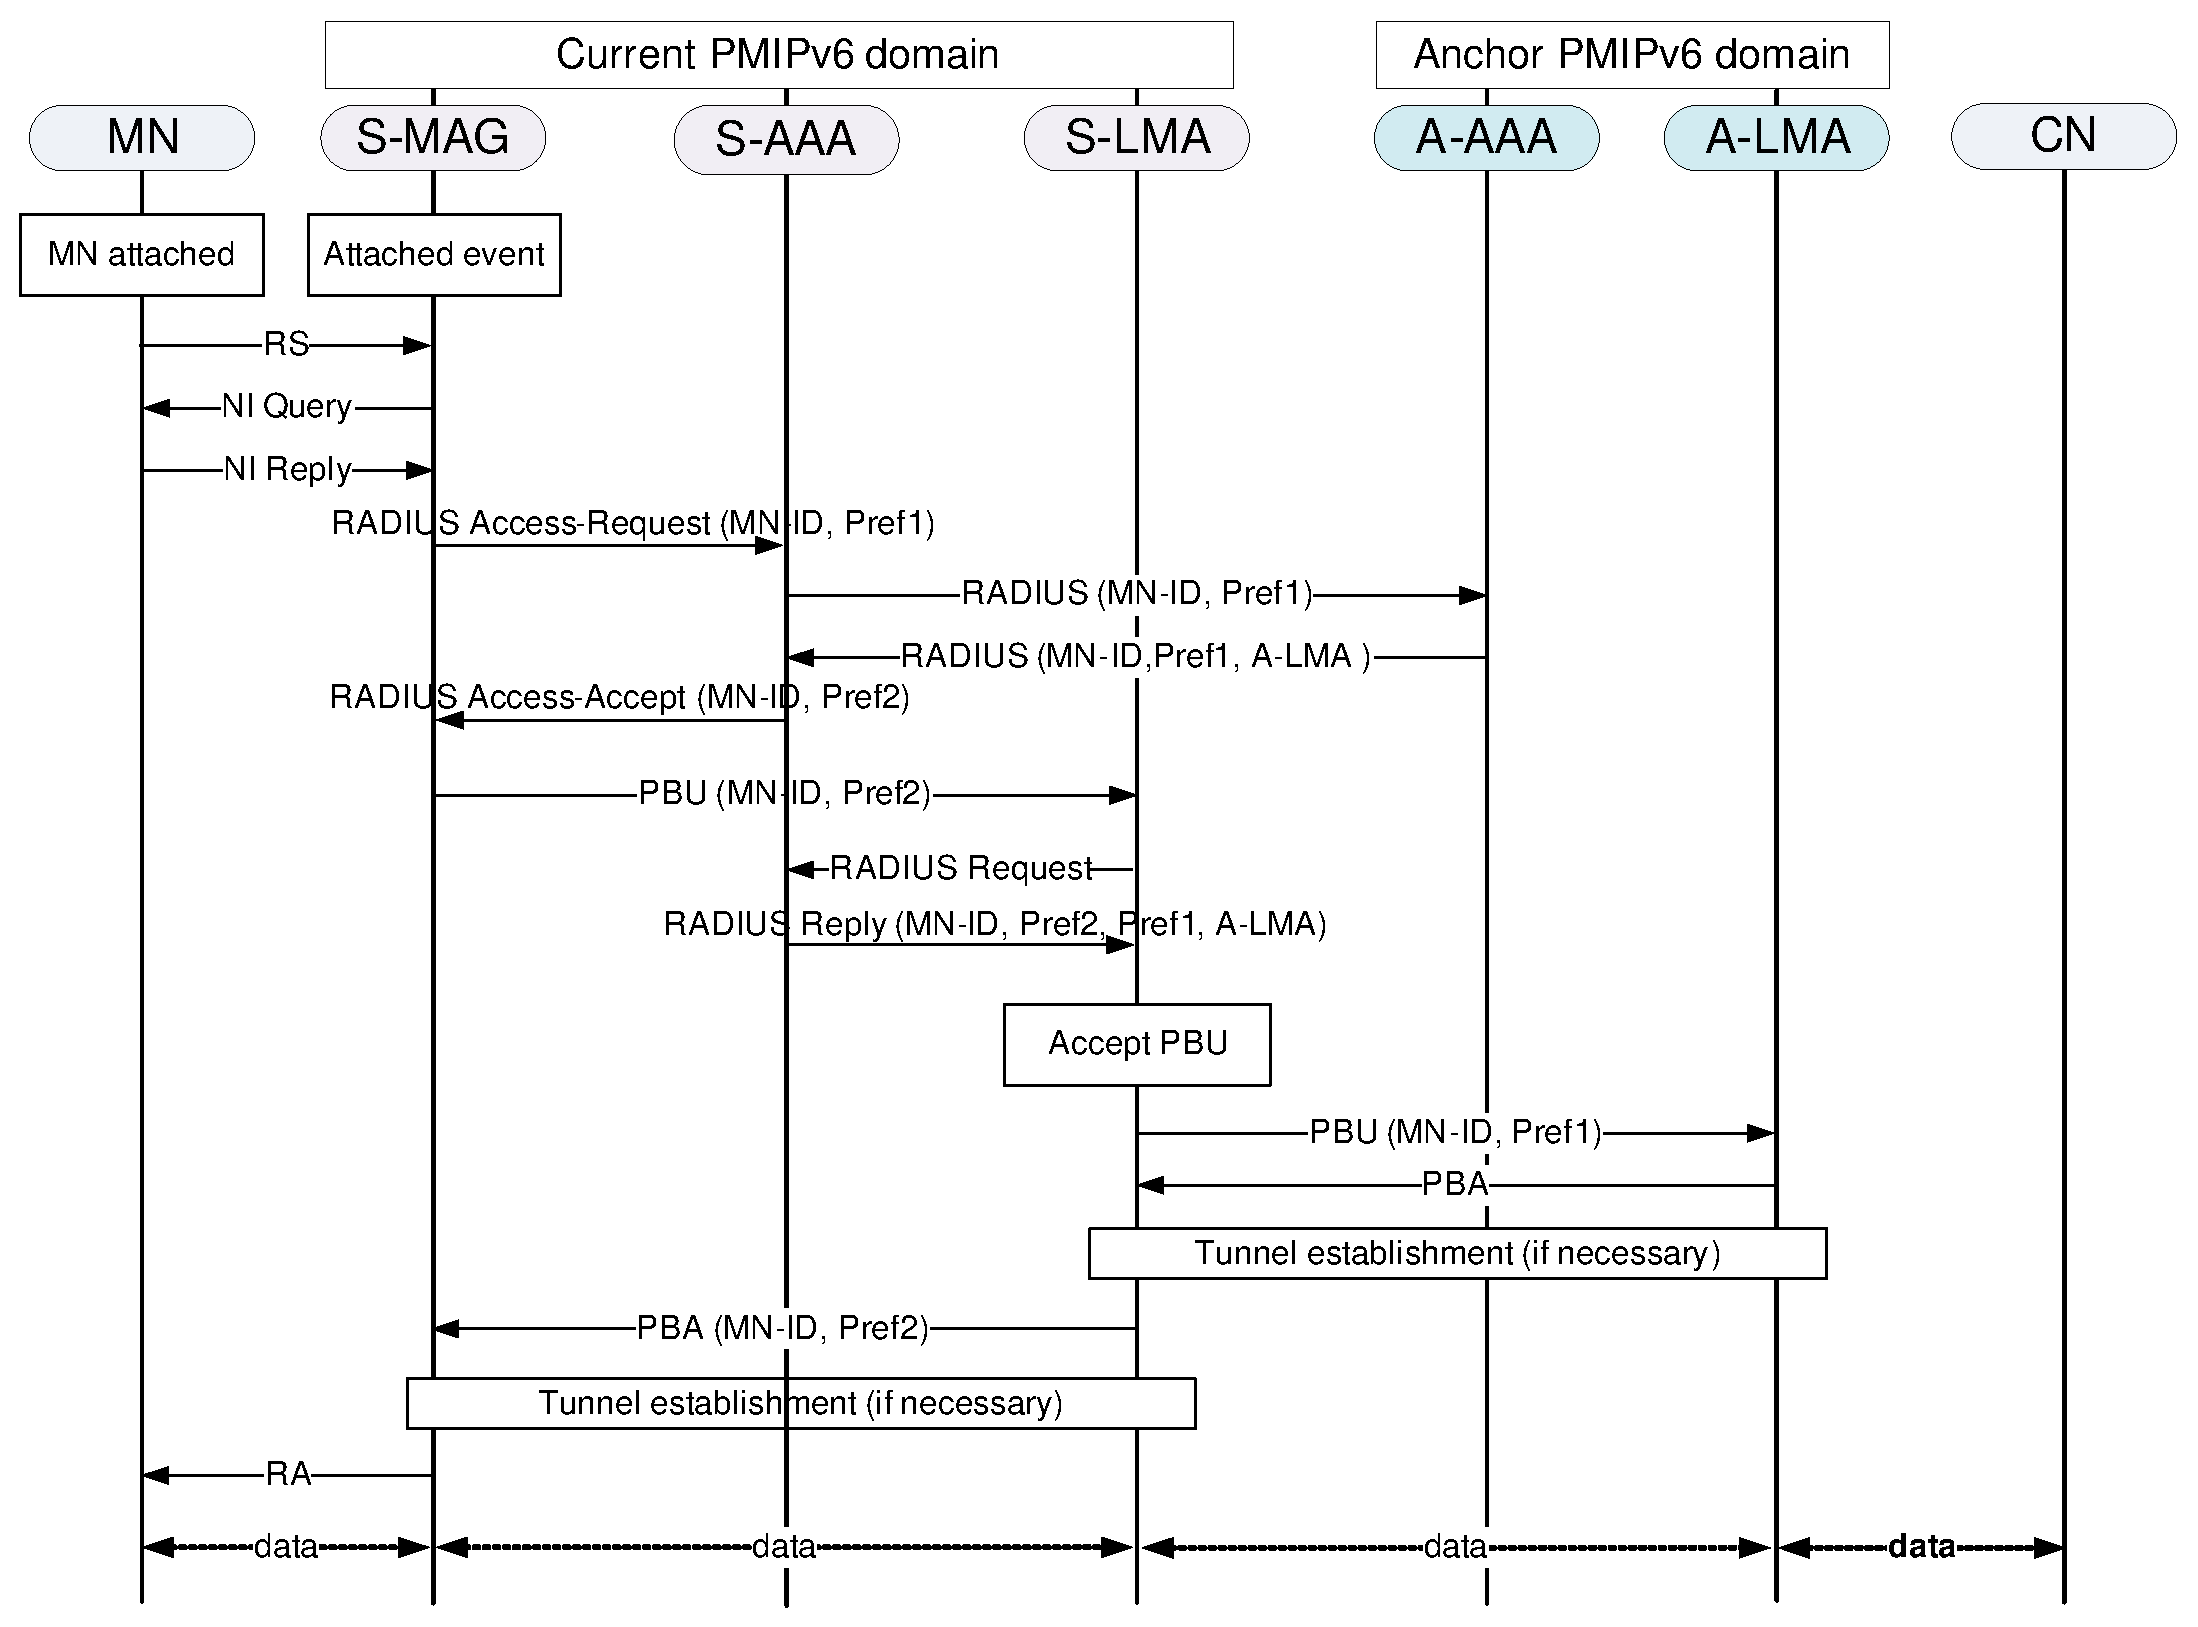
\includegraphics[width=0.95\textwidth]{./Part3/Chapter7/figures/c9_fully_distributed.eps}
\caption[Signaling for the fully distributed approach.]{Fully distributed approach (DF-PMIP).}
\label{fig:c9_fully_distributed}
\end{figure}

In this solution, the central database for inter-domain is removed from the architecture. Thus the complexity of the handover procedures is increased as a result of the trade-off between the elimination of the central database and the signaling cost. Since the S-LMA does not have knowledge of the LMAs in the other PMIPv6 domain, finding the A-LMA's address of the MN's prefix becomes a key challenge. There are several methods to solve this issue:
\begin{itemize}
\item using a Layer 2 handover infrastructure e.g., IEEE 802.21 \cite{IEEE802.21};
\item using a distributed LMA-discovery mechanism \cite{lma_discovery};
\item relying on a distributed infrastructure that allows the communication between the domains. 
\end{itemize}

In this chapter, we introduce an example to illustrate how this approach works by using a distributed Authentication, Authorization, and Accounting (AAA) infrastructure \cite{aaa2} and Remote Authentication Dial In User Service (RADIUS) protocol for PMIPv6 \cite{radius}. The protocol operations can be briefly explained as follows (see Fig.~\ref{fig:c9_fully_distributed}). 

After detecting the presence of a new MN, the current serving MAG (S-MAG) obtains the information of the MN (MN's IPv6 address) by exchanging Node Information (NI) Query/NI Reply messages \cite{rfc4620}. If the MN's IPv6 address is not available, then the normal process is executed. Vice versa, the S-MAG, after extracting the prefix from MN's address, sends a RADIUS Access-Request message with PMIPv6-Home-HN-Prefix (Pref1) and Mobile-Node-Identifier (MN-ID) options, to the AAA server (S-AAA) to retrieve the MN's policy profile. If this prefix belongs to its domain, the S-AAA then continues with its regular operations. Otherwise, acting as a RADIUS client, the S-AAA sends a RADIUS message (including MN-ID and Pref1) to the AAA in the anchor domain (A-AAA), to get A-LMA's address. Upon the reception of the RADIUS reply message from A-AAA, the S-AAA sends an Access-Accept message which includes the prefix allocated to this MN (Pref2) to S-MAG. Afterwards, the standard PMIP operations related to Pref2 are executed (e.g., location update and MN's address configuration). The S-LMA also obtains the A-LMA address from the S-AAA server. Then, the PBU/PBA messages are exchanged between the S-LMA and A-LMA to update their BCEs and routing related to Pref1. 

\subsection{Local Routing Considerations}
After the receipt of the up-link packets from MN using Pref1 as source, the S-LMA will decide to forward them to the destination depending on the following cases: (i) if the CN is currently attached to its domain, the S-LMA simply forwards the packet to the corresponding MAG; (ii) if the CN's address belongs to its domain but the CN is currently attached to another one, the S-LMA will forward the packets to the LMA that the CN is currently attached to; and iii) Otherwise, the packets will be routed following the normal internet routing. 
\subsection{Multicast Considerations}
All proposals for the inter-domain mobility support do not take multicast into account. In general, when a listener moves to a new domain, the on-going multicast flows will be interrupted. Additionally, the MN then has to re-join these flows in the new domain. Thus, the main objectives are: i) keeping the MN unaware of mobility from multicast application point of view; and ii) reducing the potential service disruption. 
In our proposed solution, multicast support can be enabled by using the multicast context transfer function and extending the PBU/PBA message to convey the multicast subscription information of the MN, as described in Fig\ref{fig:c9_multicast_signaling}. As stated in the previous section, the multicast context transfer function is developed as an independent module, which allows it to be easily integrated in any solution. 
\begin{figure}[h!]
\centering
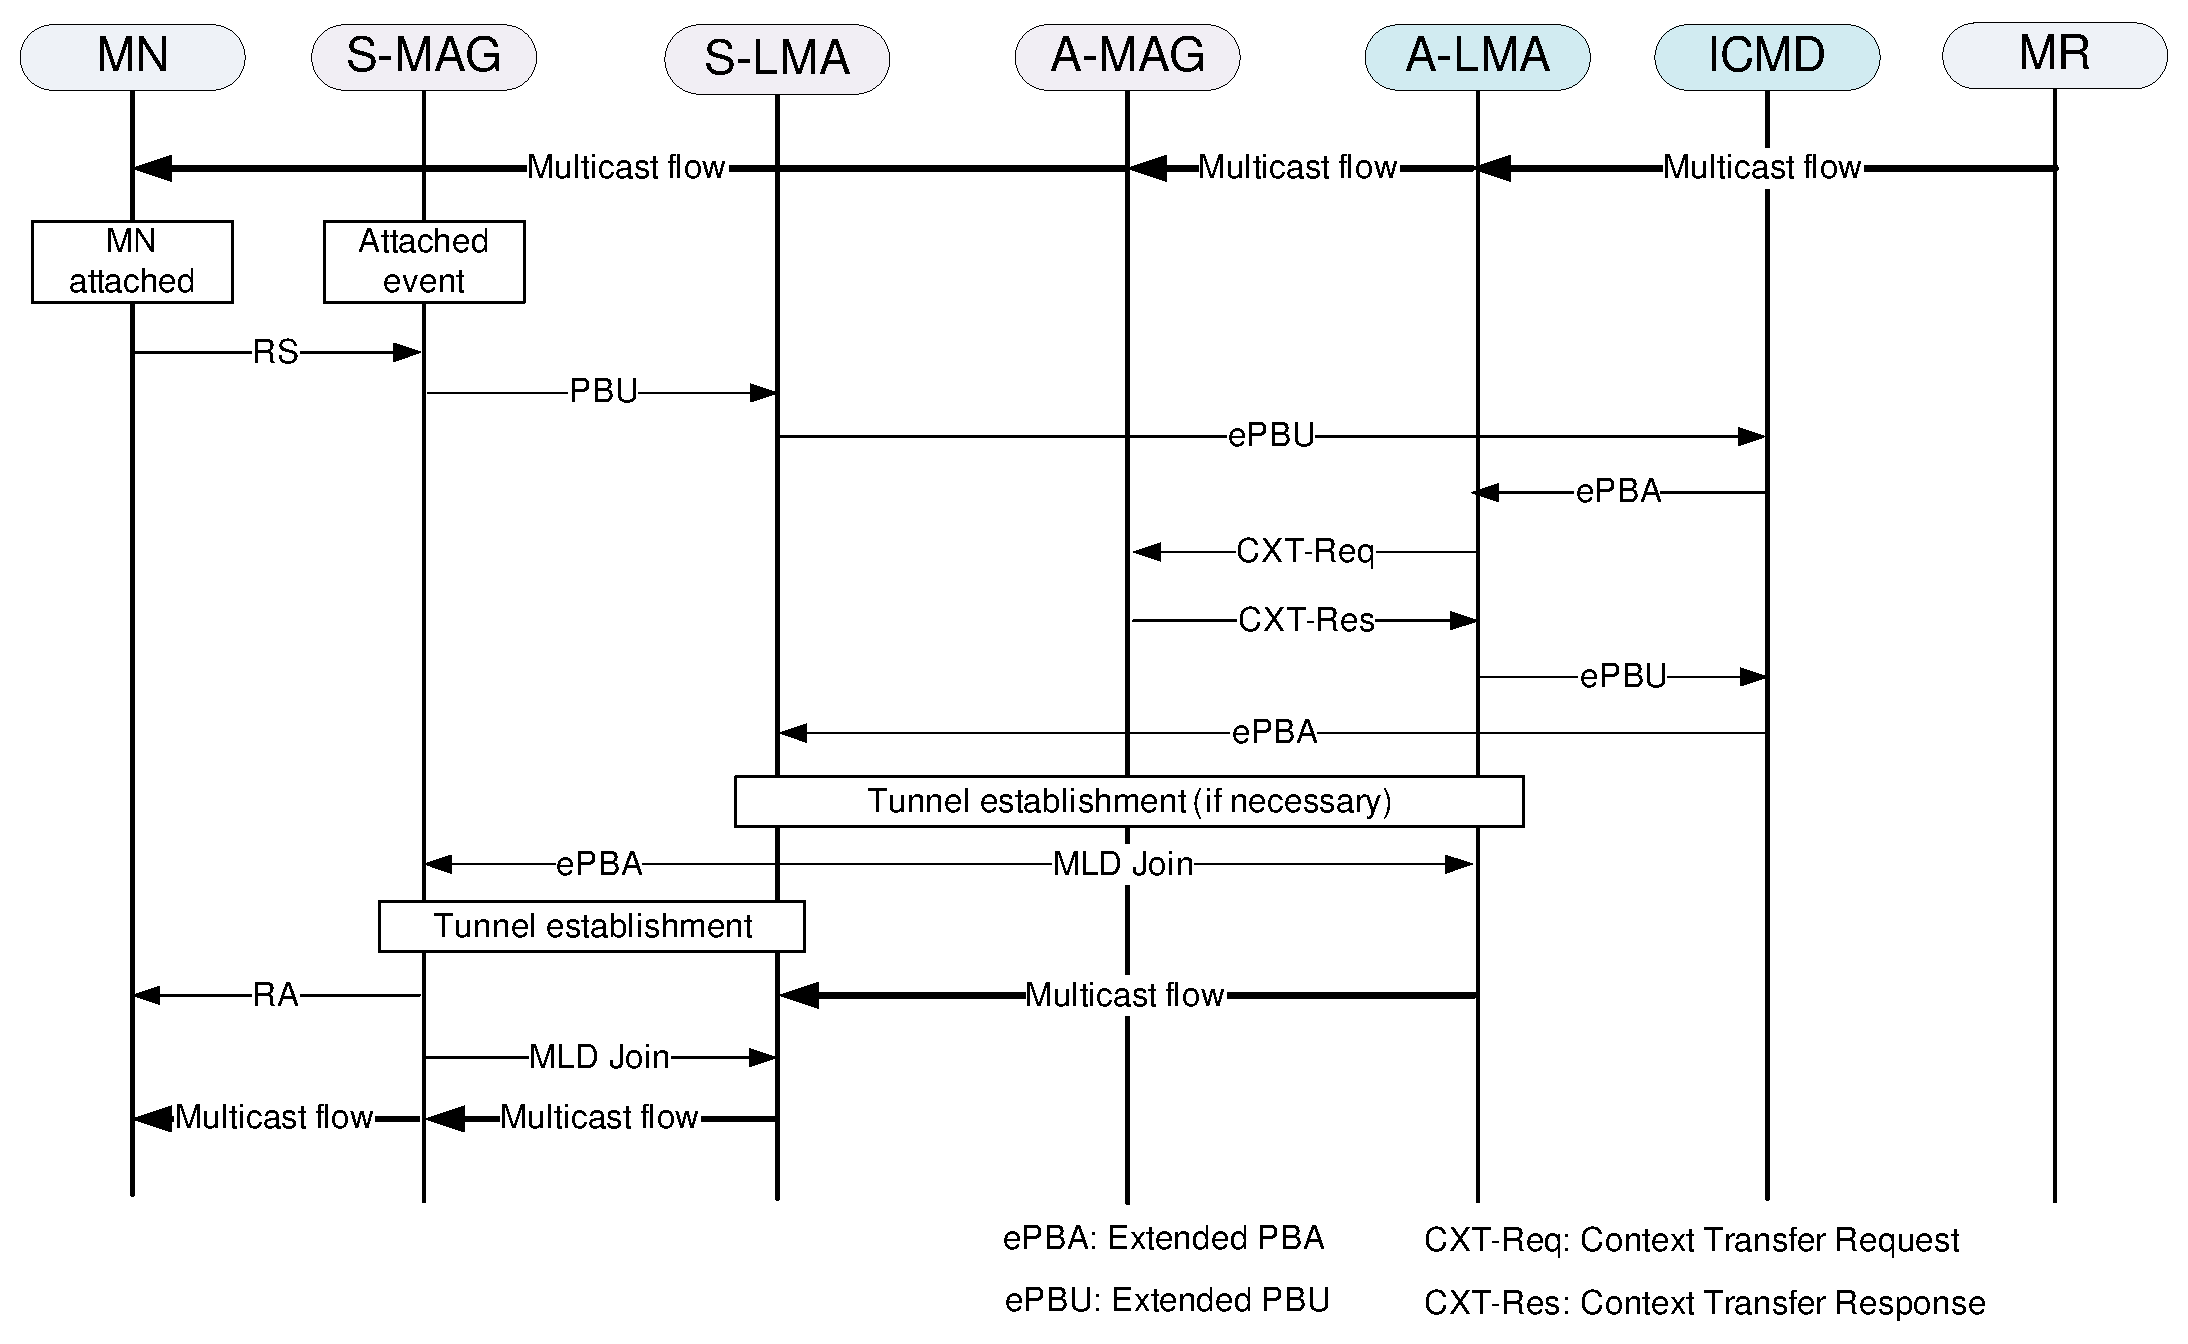
\includegraphics[width=0.85\textwidth]{./Part3/Chapter7/figures/c9_multicast_signaling.eps}
\caption[Multicast mobility support in the inter-domain mobility solution.]{Multicast mobility support in DP-PMIP.}
\label{fig:c9_multicast_signaling}
\end{figure}
The multicast-related signaling process is briefly described as follows. As stated in the previous section, upon the reception of PBU from the S-LMA, the ICMD sends a PBA to the A-LMA to update the current location of the MN. This PBA is extended to request the multicast subscription information of the MN. The A-LMA based on the context transfer function obtains the MN's subscription information from the A-MAG, and then sends it to the ICMD. The ICMD replies to the S-LMA by sending a PBA message including the MN's subscription information. The S-LMA, after establishing a tunnel with the A-LMA, sends an MLD Report to join the ongoing multicast flows of the MN via the A-LMA. The S-LMA also includes the subscription information in the PBA message to send to the S-MAG. The S-MAG, after adding the MN to a downstream interface of its MLD proxy, sends an MLD Report to the S-LMA to join these flows. Afterwards, the multicast packets are routed to the MN via the A-LMA, S-LMA and S-MAG.
\section{Performance Analysis}\label{ch9:performance_analysis}
In this section we analyze the performance of the proposed solutions in terms of signaling cost, handover latency and tunnel usage. We compare our solutions with the other ones for the inter-domain handover e.g., MIPv6, H-PMIP and I-PMIP. 
\subsection{Reference Model}
\begin{figure}[h!]
\centering
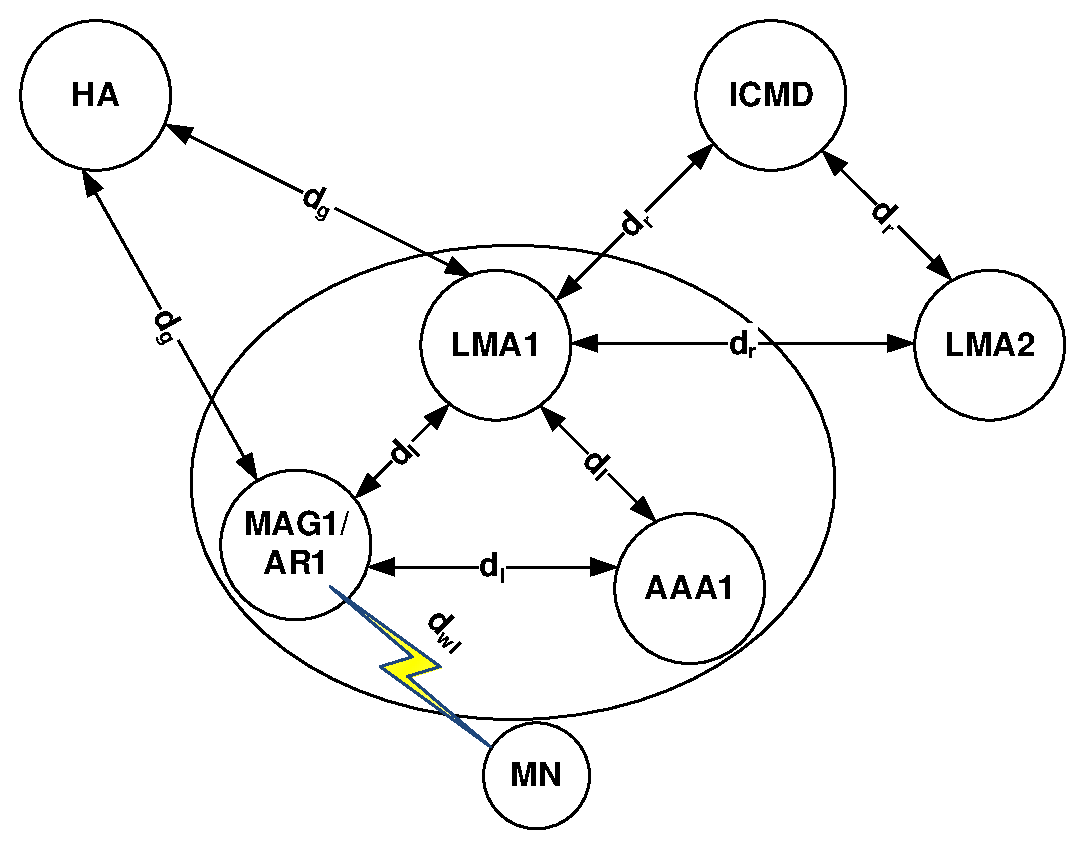
\includegraphics[width=0.55\textwidth]{./Part3/Chapter7/figures/c9_topology_analysis.eps}
\caption[Reference network topology for performance analysis.]{Reference network topology for performance analysis.}
\label{fig:c9_reference}
\end{figure}

Fig.~\ref{fig:c9_reference} shows a reference topology for performance analysis. For simplicity, the average distance (number of hops) between the entities is defined as follows:
\begin{itemize}
\item The distance between the PMIPv6 entities in the same domain (local) is d$_{l}$ (e.g., between the MAG and the LMA). 
\item The distance between two domains (region) is d$_{r}$ (e.g., between two LMAs or between the LMA and the ICMD).
\item The distance between LMA/AR and Home Agent (HA) (global) is d$_{g}$.  
\item The distance between the MAG/AR and the MN (wireless connection) is d$_{wl}$.
\end{itemize}

\subsection{Signaling Cost}
Signaling cost of a mobility management protocol is defined as the transmission cost of location update signaling when an MN performs handover. To measure the signaling cost in the inter-domain context, the handoff frequency should be taken into account. As a result, we use a well-known factor, called session-to-mobility ratio (SMR) which represents the relative ratio of session arrival rate to the user mobility rate.
It is assumed that the subnet residence time (MAG subnet) and session duration follows an exponential distribution with parameter $\eta$ and $\mu$, respectively. Hence, the SMR is calculated as $\rho=\frac{\mu}{\eta}$ \cite{prob}. 
Each LMA coverage area is supposed to be circular with N subnets. According to \cite{HO_comparison_Makaya}, the intra-domain and the inter-domain handoff probability are defined as $\rho_{intra}=\frac{1}{1+\rho}$,  $\rho_{inter}=\frac{1}{1+\rho \sqrt{N}}$. And the expected numbers of intra-handoff and inter-handoff are $E_{intra}=\dfrac{1}{\rho}$, $E_{inter}=\dfrac{1}{\rho \sqrt{N}}$
Thus, the average location update signaling is given by:\\
\begin{equation}
SC(.) = \left( E_{intra} - E_{inter}\right) SC_{intra} (.) + E_{inter} SC_{inter}(.),
\end{equation}
where $SC_{intra}$ and $SC_{inter}$ are signaling update cost for intra-domain and inter-domain handover, respectively. 
Although different signaling messages have different size, we assume that they have the same size for simplicity. Also, the cost for transmitting a signaling message is supposed to be proportional to the distance between source and destination. The proportion is $\alpha$ for wired and $\beta$ for wireless link. The signaling cost of DP-PMIP is calculated as: 
\setlength{\arraycolsep}{0.0em}
\begin{eqnarray}
SC_{intra} (DP-PMIP)&{}  ={}& 2 \beta d_{wl} + 2\alpha d_{l},\\
SC_{inter}(DP-PMIP)&{}  ={}&  2 \beta d_{wl} + 2\alpha d_{l} +4\alpha d_{r}. 
\end{eqnarray}

Similarly, we can derive the equations of the signaling cost for DF-PMIP, MIPv6 and H-PMIP. It is noted that the signaling cost for intra-domain handover of DF-PMIP and H-PMIP is the same and equal to that of DP-PMIP (PMIP handover cost). \\
\setlength{\arraycolsep}{1.0em}
\begin{eqnarray}
SC_{inter}(DF-PMIP)&{} ={}& 4\beta d_{wl} + 6\alpha d_{l} +4\alpha d_{r}. \\
SC_{inter}(MIP)&{} ={}& SC_{intra}(MIP) = 4 \beta d_{wl} + 2\alpha d_{g}. \\
SC_{inter}(H-PMIP)&{} ={}& 4\beta d_{wl} + 2\alpha d_{l} +2\alpha d_{g}.
\end{eqnarray}

\subsection{Handover Latency}
The Inter-domain handover latency ($HO_{inter}$) is defined as the total time taken to complete all the operations before the traffic can be forwarded to the current location of the MN. Let $HO_{intra}$ denote the intra-domain handover delay. Then, the average value of handover latency is
\begin{equation}
\label{DP-PMIP}
HO(.)  = \left( \rho_{intra} - \rho_{inter} \right) HO_{intra}(.) + \rho_{inter} HO_{inter}(.).
\end{equation}

Since the delay between two nodes depends on the bandwidth, the propagation delay and the distance between them, for simplicity, we suppose that the delay is proportional to the distance. The proportion is $ \tau$ for wired link and $\kappa$ for wireless link. 
Let t$_{L2}$ denote the delay caused by Layer 2 handover. Thus, the intra-domain handover delay of DP-PMIP, DF-PMIP and H-PMIP are the same (PMIP handover delay) and are calculated as follows:\\
\begin{equation}
\label{DP-PMIP-intra}
HO_{intra}(DP-PMIP) = t_{L2} + 2\kappa d_{wl} + 2\tau d_{l}. 
\end{equation}

On the other hand, the handover latency of DP-PMIP, DF-PMIP, MIPv6 and H-PMIP are given by the equations below.\\
\setlength{\arraycolsep}{0.0em}
\begin{eqnarray}
HO_{inter}(DP-PMIP)&{} ={}& t_{L2} + 2 \kappa d_{wl} + 2\tau d_{l} + 2\tau d_{r}. \\
HO_{inter}(DF-PMIP)&{} ={}& t_{L2} + 4 \kappa d_{wl} + 6\tau d_{l}+ 4\tau d_{r}. \\
HO_{inter}(MIP)&{} ={}& SD_{Intra}(MIP) = t_{L2} + 4\kappa d_{wl} + 2\tau d_{g}. \\
HO_{inter}(H-PMIP)&{} ={}& t_{L2} + 4\kappa d_{wl} + 2\tau d_{r} + 2\tau d_{g}. 
\end{eqnarray}
\subsection{Tunnel Usage}
In this subsection, we will measure the tunnel usage ratio, called $\theta$ which is calculated as the ratio between the number of sessions using the tunnel (between the anchor and the current domain) and the total number of sessions. Thus, it can be used to show the advantage of using DMM in terms of dynamic provision of mobility service. 

Since in MIPv6, H-PMIP and I-PMIP the traffic always passes the tunnel between the global anchor point and the current one, $\theta$ is equal to 1. 

To measure $\theta$ in case of D-PMIP, the sessions are separated into new sessions and handoff sessions. Thanks to DMM, the tunnel is used only for the handoff sessions. Let $N_{n}(t)$ and $N_{h}(t)$ denote the numbers of new sessions and handoff sessions up to time t, respectively. We suppose that $N_{n}(t)$ and $N_{h}(t)$ are a Poisson process with parameter $\lambda_{n}$ and $\lambda_{h}$, respectively. Thus, we have $\theta =\dfrac{N_{h}(t)}{N_{n}(t)+N_{h}(t)}$. According to \cite{prob} $\lambda_{h} = E[H] * \lambda_{n}$, where E[H] is the handoff rate (in our case E[H] = $\frac{1}{\rho\sqrt{N}}$). 
Thus, we obtain:
\begin{equation}
\theta = \dfrac{1}{ 1+ \rho\sqrt{N}}.       
\end{equation}

\subsection{Multicast Service Disruption Time}
Similar to the handover latency, the multicast service disruption time ($SD(.)$) is defined as\\
 \begin{equation}
SD(DP-PMIP)= \left( \rho_{intra} - \rho_{inter} \right) SD_{intra}(DP-PMIP) + \rho_{inter} SD_{inter}(DP-PMIP),
\end{equation}
where $SD_{intra}(DP-PMIP)$ and $SD_{inter}(DP-PMIP)$ are the multicast service disruption time for intra- and inter-domain mobility, respectively. As can be seen in Fig.~\ref{fig:c9_multicast_signaling}, $SD_{inter}(DP-PMIP)$ is calculated as\\
\begin{equation}
SD_{inter}(DP-PMIP) = t_{L2} + 2\kappa d_{wl} + 4\tau d_{l} + 4\tau d_{r} + 2 max \{ \tau d_{l}, \tau d_{r} \}. 
\end{equation}
The multicast service disruption, in case of intra-domain handover is given by (see Chapter \ref {ch:multicast_PMIP})
\begin{equation}
SD_{intra}(DP-PMIP) = t_{L2} + 2 \kappa d_{wl} + 6\tau d_{l}. 
\end{equation}

On the other hand, the average multicast service disruption time in PMIPv6 is given by\\
\begin{equation}
SD(PMIP) = \rho_{intra} SD_{intra}(DP-PMIP). 
\end{equation}

\section{Numerical Results} \label{ch9:numerical_result}
This section presents the numerical results based on the analysis given in the previous section. The default parameter values for the analysis are introduced in Table ~\ref{tap:c9_parameters} in which some parameters are taken from \cite{HO_comparison_Makaya}. \\

\begin{table}[ht]
\caption[Inter-mobility domain solution: Parameters for the performance analysis]{Parameters for Performance Analysis}
\label{tap:c9_parameters}
\centering
\begin{tabular}{|c |c |c |c |}
\hline
Parameters & Values & Parameters & Values\\
\hline
d$_{wl}$ & 1 hops &d$_{l}$ & 6 hops \\
\hline
 d$_{r}$ & 6 hops & d$_{g}$ & 12 hops \\
 \hline
$\tau$ & 2 & $\kappa$ & 15  \\
\hline
N & 32 & $\alpha$ & 1 \\
\hline
$\beta$ & 5  & $t_{L2}$ & 50ms \\
\hline

\end{tabular}
\end{table}

\begin{figure}[h!]
\centering
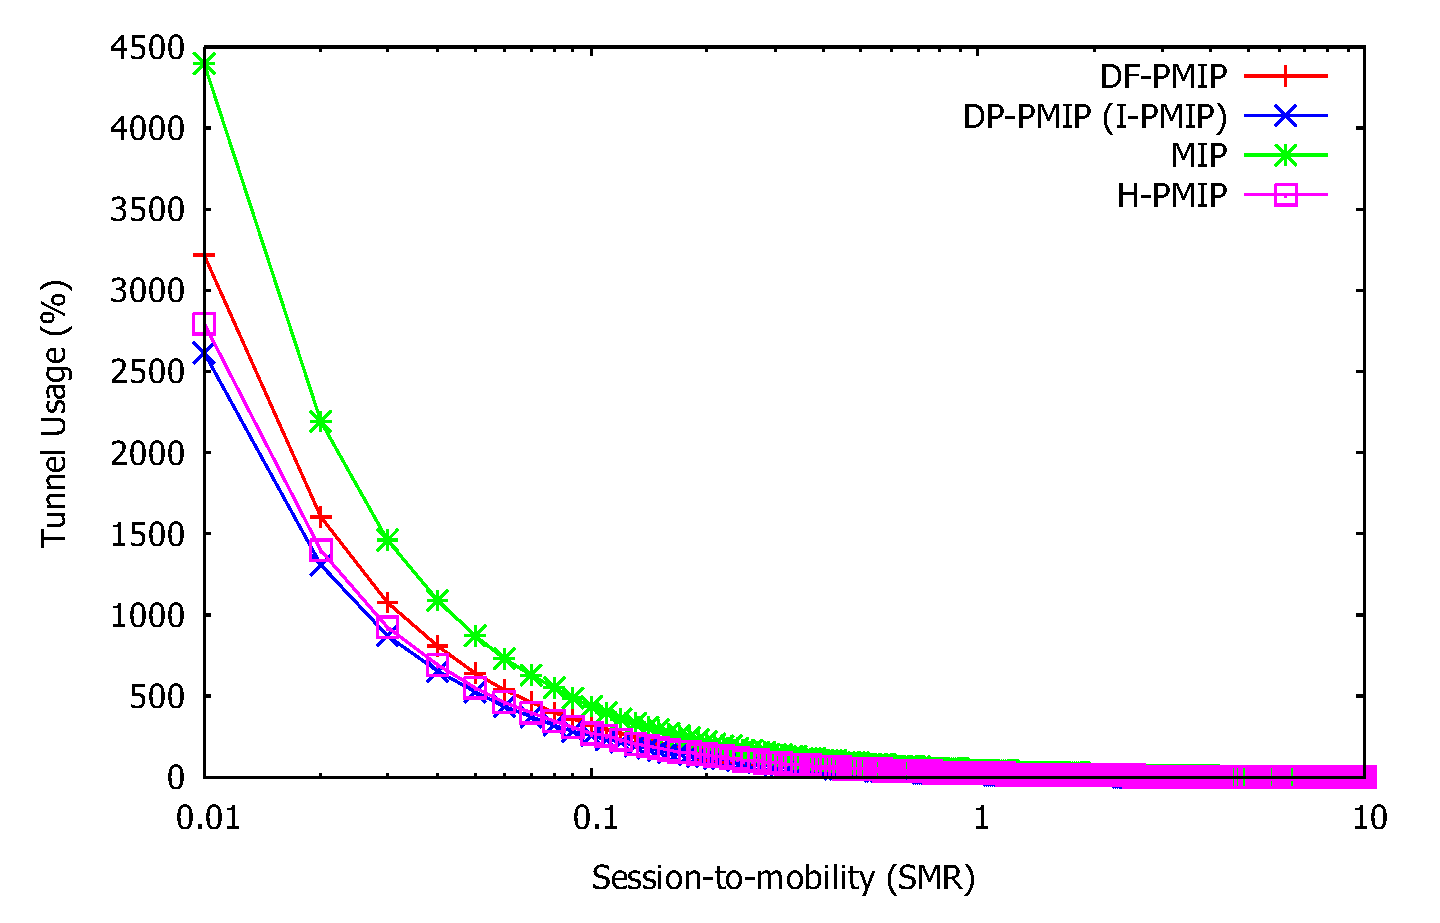
\includegraphics[width=0.50\textwidth]{./Part3/Chapter7/figures/c9_signaling_cost_smr_6.eps}
\caption[Signaling cost as a function of the session-to-mobility.]{Signaling cost variation with SMR ($\rho$).}
\label{fig:signaling_cost}
\end{figure}

Fig.~\ref{fig:signaling_cost} shows the signaling cost when SMR ($\rho$) is varying. We can observe that the signaling cost of the fully distributed solution is relatively high compared to the other. It is evident since more messages are required to get the address of the anchor LMA. The partially distributed solution and I-PMIP have lower signaling cost than that of the others. In highly mobile regimes ($\rho\ll1$), the difference between the protocols becomes more clearly. 

Fig.~\ref{fig:Handover_latency} illustrates the handover latency as a function of SMR. The partially distributed solution (DP-PMIP) has better handover latency (lower is better) over the other solutions especially when $\rho$ is small (in highly mobile regimes). 
\begin{figure}
\centering
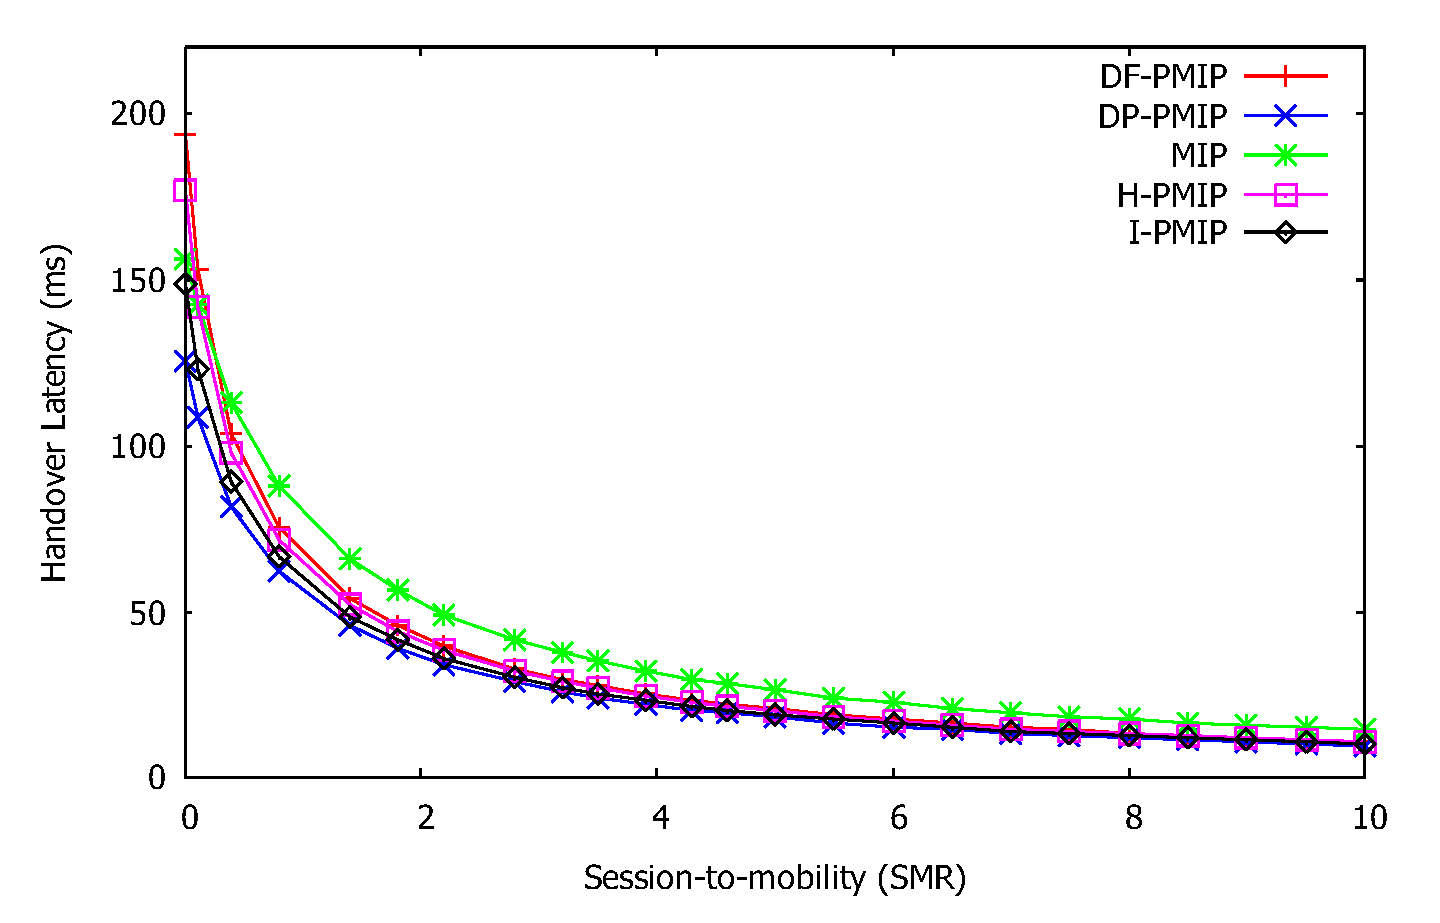
\includegraphics[width=0.50\textwidth]{./Part3/Chapter7/figures/c9_handover_smr_6.eps}
\caption[Handover latency as a function of the session-to-mobility.]{Handover latency variation with SMR ($\rho$).}
\label{fig:Handover_latency}
\end{figure}

To measure the impact of domain size on the handover latency, we assume that the architecture of the inter-domain is hierarchically formed as a tree structure with a $d_{r}$-layer, while the structure of a PMIPv6 domain as a binary tree with a $d_{l}$-layer \cite{multicast_mobileIP}. The size of the network is supposed to be fixed e.g., the distance between the ICMD and MAG is 12 hops. Therefore, $d_{l}$ and $d_{r}$ are calculated as $d_{l}=log_{2}(N)$, $d_{r} = 12 - log_{2}(N)$. Fig.~\ref{fig:domain_size} describes the impact of domain size on handover latency when the value of $\rho$ is set to 0.1. It is observed that when the domain size is small, the handover latency is high for all solutions. When the domain size is increased, the handover latency is decreased and then makes a bit increase. 
\begin{figure}[h!]
\centering
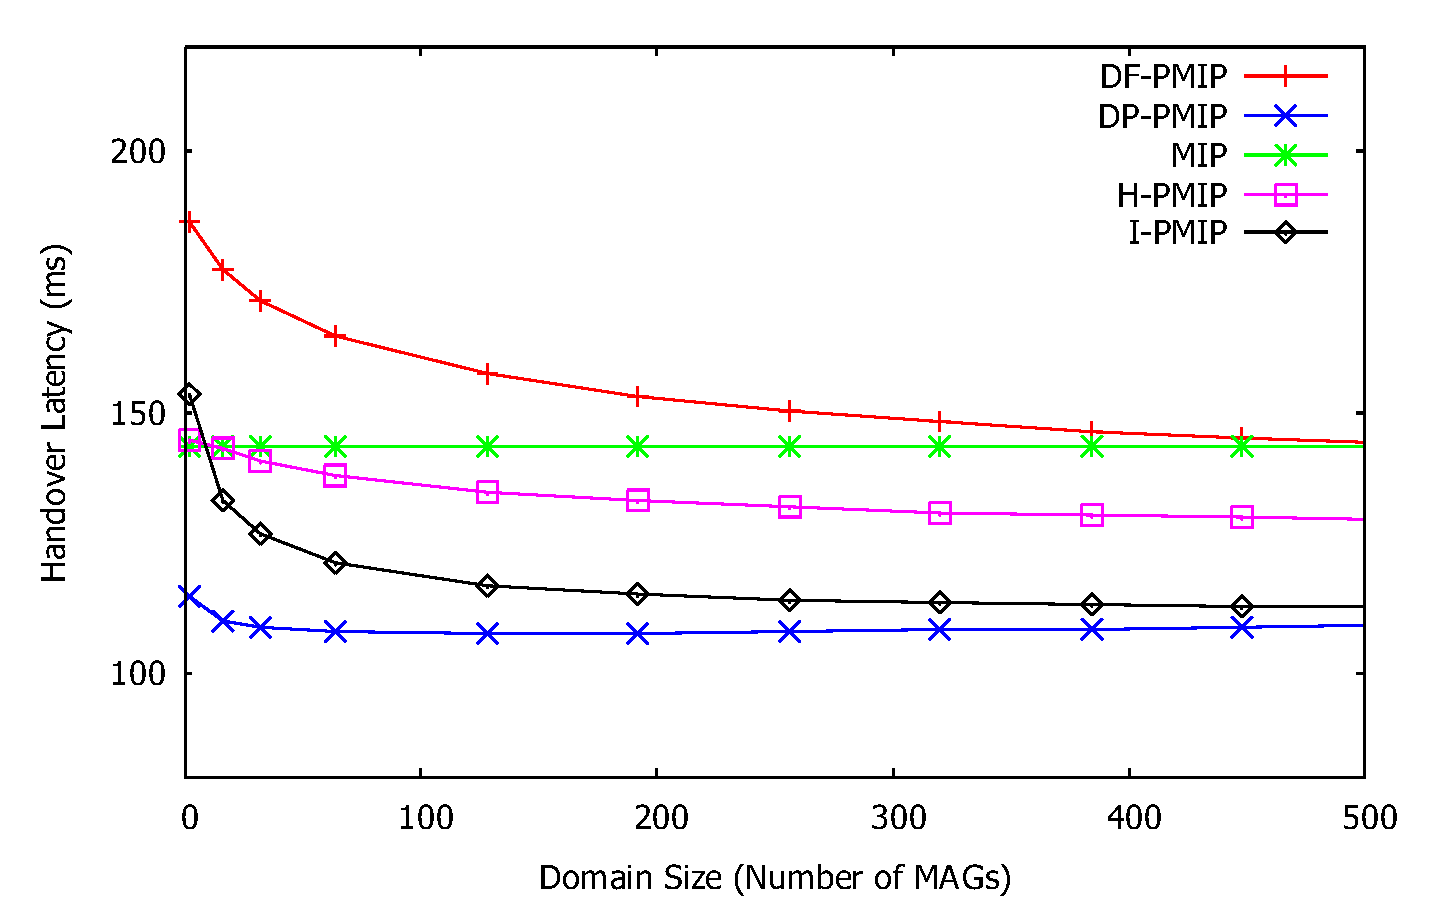
\includegraphics[width=0.50\textwidth]{./Part3/Chapter7/figures/c9_domain_size_6.eps}
\setlength{\belowcaptionskip}{-10pt}
\caption[The impact of domain size on the handover latency.]{Domain size effect.}
\label{fig:domain_size}
\end{figure}

The tunnel usage as a function of SMR is illustrated in Fig.~\ref{fig:tunnel_usage}. In low mobility regimes ($\rho\gg1$) the tunnel usage is significantly decreased in D-PMIP (DP-PMIP, DF-PMIP) compared to the others. The reason is that the number of new sessions in low mobility regimes is definitely higher than that of handoff sessions.
\begin{figure}[h!]
\centering
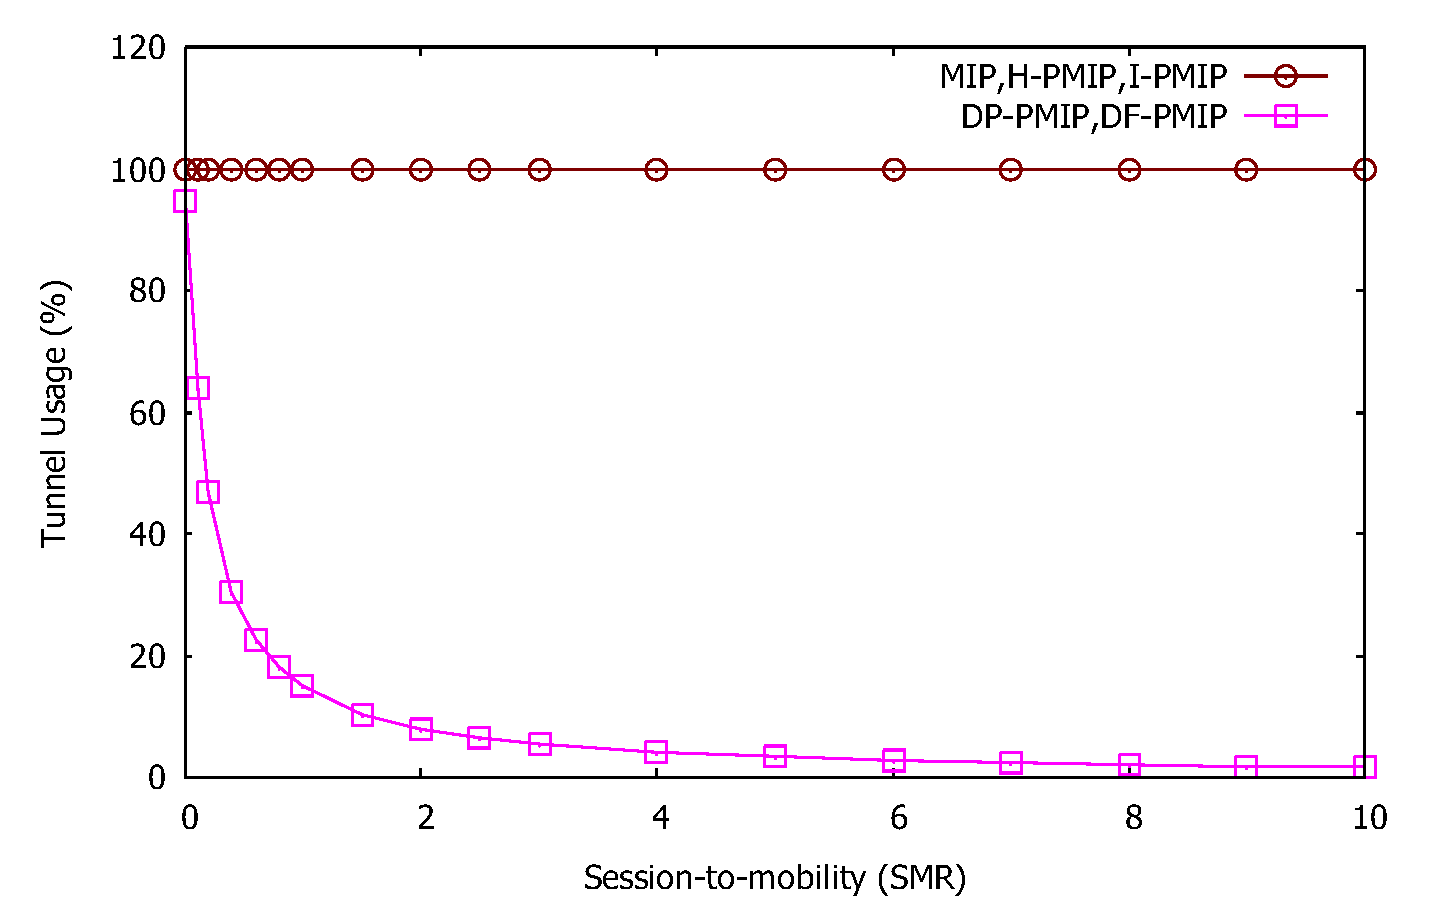
\includegraphics[width=0.50\textwidth]{./Part3/Chapter7/figures/c9_tunnel_usage.eps}
\caption[Tunnel usage.]{Tunnel usage ($\theta$) as a function of SMR ($\rho$).}
\label{fig:tunnel_usage}
\end{figure}

Finally, Fig.~\ref{fig:multicast} plots the average multicast service disruption time as a function of SMR. We can observe that the average service disruption in case of DP-PMIP is slightly greater than that in case of intra-handover inside PMIPv6. It is because inter-domain handover latency is typically greater than that in case of intra-domain handover. 

\begin{figure}[h!]
\centering
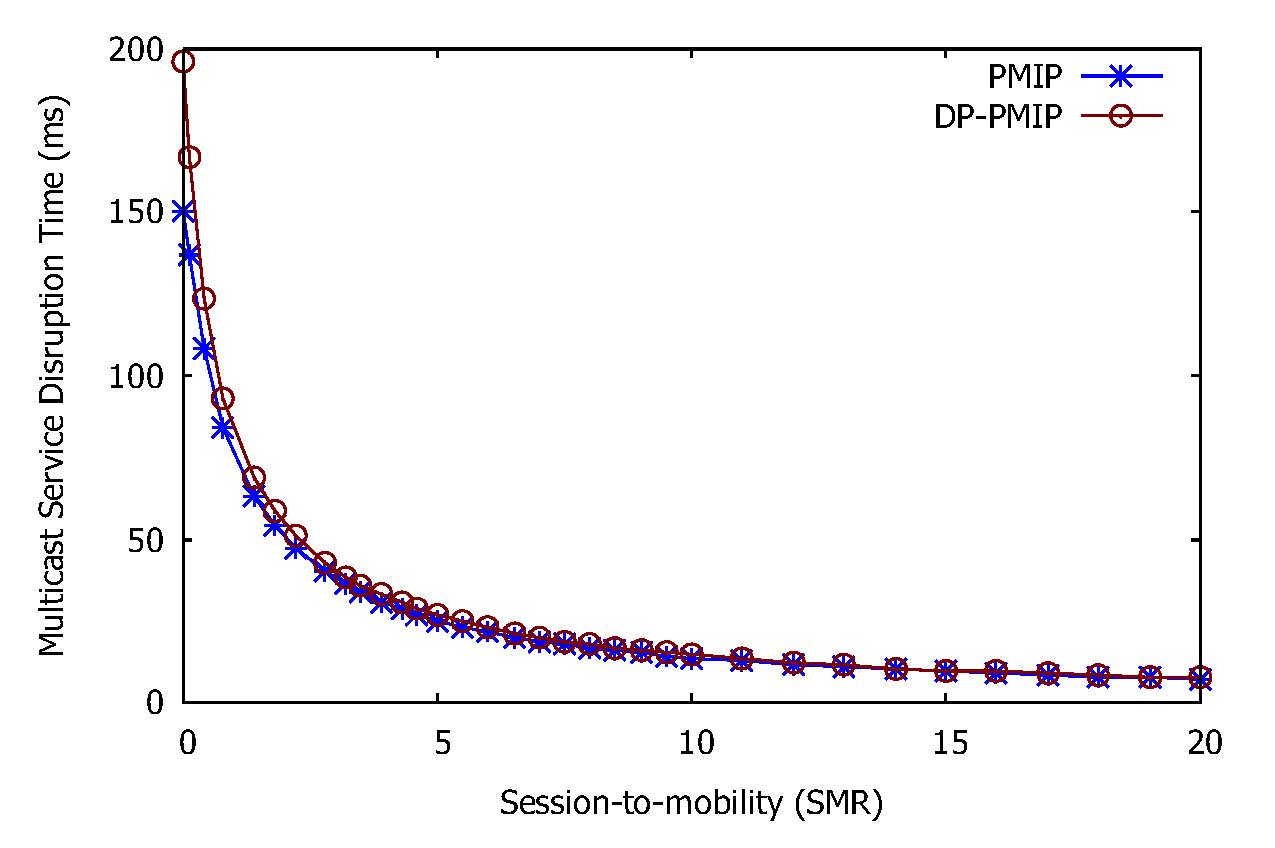
\includegraphics[width=0.50\textwidth]{./Part3/Chapter7/figures/c9_multicast.eps}
\caption[Multicast service disruption time as a function of the session-to-mobility.]{Multicast service disruption time as a function of SMR ($\rho$).}
\label{fig:multicast}
\end{figure}

\section{Conclusion} \label{ch9:conclusion}
This chapter proposes a solution (D-PMIP) that allows providing mobility service for the moving hosts between PMIPv6 domains. Based on the DMM concept, the proposal allows bringing the mobility anchors closer to the MN and dynamically providing the mobility service for only sessions which really need the service continuity. The D-PMIP also retains the advantageous features of a network-based mobility management form PMIPv6 that provides mobility service without the involvement of the MN. A numerical analysis demonstrates that the partially distributed solution gives better performance than the other solutions like MIPv6, H-PMIP, I-PMIP and the fully distributed solution in terms of signaling cost, handover latency and tunnel usage. Thus, at the moment the partially distributed solution seems to be more suitable than the fully distributed one. 

The proposed solutions can be considered as a DMM-like approach applying to the existing PMIPv6 network to improve the mobility of the nodes. We then present a basic support for the multicast mobility in the partially distributed scheme. It allows keeping the MN unaware of mobility from the multicast service perspective. Also, the multicast service disruption time is slightly increased compared to the mobility inside a single PMIPv6 domain. 


\chapter{On the Efficiency of Dynamic Multicast Mobility Anchor in DMM} \label{ch:multicast_dmm}
As stated in the previous chapter, IP multicast can be enabled in DMM by deploying the MLD proxy function at MAR. The multicast traffic is routed directly from the native multicast infrastructure via the current MAR for the new multicast flow. For the flow after handover, the multicast traffic is tunneled from the MAR where the flow is initiated to the current one via the mobility tunnel between them. Thus, the multicast mobility anchor (MMA) is assigned at the initial phase of the multicast flow (identical with the unicast mobility anchor): the MAR where the flow is initiated. The multicast flow will be anchored at the initially assigned MMA during its lifetime. Therefore, even when the MN moves far away from its anchor, the multicast traffic still traverses the anchor. As a result, it causes several issues to the ongoing multicast flow such as service disruption, non-optimal routing, end-to-end delay and packet duplication. These problems become serious when considering the interruption- and delay-sensitive services. Also, even the mobility anchors are distributed, some anchors are more overloaded than the others \cite{anchor_selection}.

In this chapter, we mainly argue the need for a dynamic multicast mobility anchor (DMMA) mechanism. From a service point of view, it helps satisfy the requirements in terms of service disruption and delay, especially when considering the real-time services. It provides a mechanism to better distribute the load among MARs. Moreover, other issues like packet duplication and leave latency (waste of resource) can be reduced. The DMMA takes into account not only the multicast service context (e.g., interruption-sensitive and delay-sensitive services) but also the mobile node's mobility context and the network context (such as current load of MARs and multicast channel policy), thus enabling a per-flow multicast support. In other words, each multicast flow can be treated differently upon different contexts. 

The rest of this chapter is organized as follows. Section \ref{c10:multicast_listener} introduces the issues and different approaches for the multicast listener support in a DMM environment. Section \ref{c10:quantitative_analysis} presents the performance analysis regarding different metrics as service disruption, end-to-end delay, signaling cost and packet loss. The DMMA mechanism is presented in Section \ref{c10:dmma}. Section \ref{c10:discussion} discusses the implementation work, the scenario in which the multicast router is deployed at MAR as well as the multicast source support. Finally, Section \ref{c10:conclusion} concludes this chapter and provides perspectives for future work. 

\section{Multicast Listener Mobility in DMM} \label{c10:multicast_listener}

This chapter follows the concept of the network-based DMM proposed by the IETF DMM Working Group\footnote{http://datatracker.ietf.org/wg/dmm/} as described in Chapter \ref{ch:reference_technologies}. We recall some abbreviations introduced in the previous chapters to denote the role of MAR from a mobile node point of view:
\begin{itemize}
\item Current MAR (cMAR) is the MAR to which the MN is currently attached.
\item Anchor MAR (aMAR) of an MN's address/session is the MAR where the prefix in use is allocated (and the session is initiated using this address as the source address).  
\item Previous MAR (pMAR) is the MAR where the MN was previously attached. 
\end{itemize}

As mentioned in Chapter \ref{ch:reference_technologies}, there is a limited work for the multicast support since the DMM is still in an early stage of standardization.  This chapter focuses on the scenario in which the MAR acts as an MLD proxy. Also, only multicast listener mobility in the network-based DMM is further studied. In this case, when a multicast flow is initiated, the multicast traffic is received directly from the native multicast infrastructure via the cMAR. After handover, the traffic is routed from the anchor to the current MAR via the tunnel between them (like unicast traffic). In this chapter, it is called the default multicast mode in DMM. However, this mode does not address any multicast-related issues caused by the movement of listener such as service disruption, packet loss, non-optimal routing, end-to-end delay, and tunnel convergence problem (for further information, see Chapter \ref{ch:reference_technologies}). 

Regarding the service disruption, when a multicast listener moves from the pMAR to the cMAR, it may cause a noticeable service disruption for the ongoing flows. As a result, the multicast context transfer is required to avoid a large delay caused by multicast-related procedures (about 5s in the normal case, and 2.5s in the best case) \cite{Thinh_WCNC_Multicast}. This delay is much longer than the maximum tolerant interruption time for normal services, as specified in \cite{interruption_requirements} is 500 ms. Even with the multicast context transfer, it is unable to meet the requirement in terms of service disruption for the interruption-sensitive service when the delay cMAR-aMAR is large \cite{Thinh_ICNS, multicast_DMM_Sergio_PIMRC}. It is because the multicast traffic has to pass through the aMAR, which plays the role of multicast mobility anchor (MMA).  

Also, since the multicast traffic always traverses the aMAR, it often results in a longer route (e.g., when the source and the listener are close to each other but far from the listener's aMAR). In particular, when considering a significant large domain, it can cause a high end-to-end delay. This issue becomes serious when the end-to-end delay sensitive service is considered. 

In case of mobility, the utilization of the mobility tunnel for the multicast flow may result in the tunnel convergence problem. It occurs when multiple instances of the same multicast traffic converge to an MAR, leading to the redundant traffic. The main reason is that multiple MLD proxy instances are installed at MAR with their upstream interfaces configured to different aMARs. Since the purpose of DMM is moving the mobility anchors from the core to the edge of the networks, the number of mobility anchors in a DMM domain will be much more than that in a PMIPv6 domain. As a consequence, the tunnel convergence problem is supposed to be much more severe than that in PMIPv6. As stated in the DMM requirements \cite{DMM_requirements}, the multicast solutions in DMM should take this issue into consideration. By using an extension to MLD proxy to support multiple upstream interfaces \cite{multiple_upstreams}, the tunnel convergence problem can be avoided. In this case, only one proxy instance will be installed at MAR with its upstream interfaces being configured towards different aMARs and its upstream MR. Accordingly, the MAR will receive only one instance of the multicast packet.
\begin{figure}[tb!] 
  \begin{center} 
    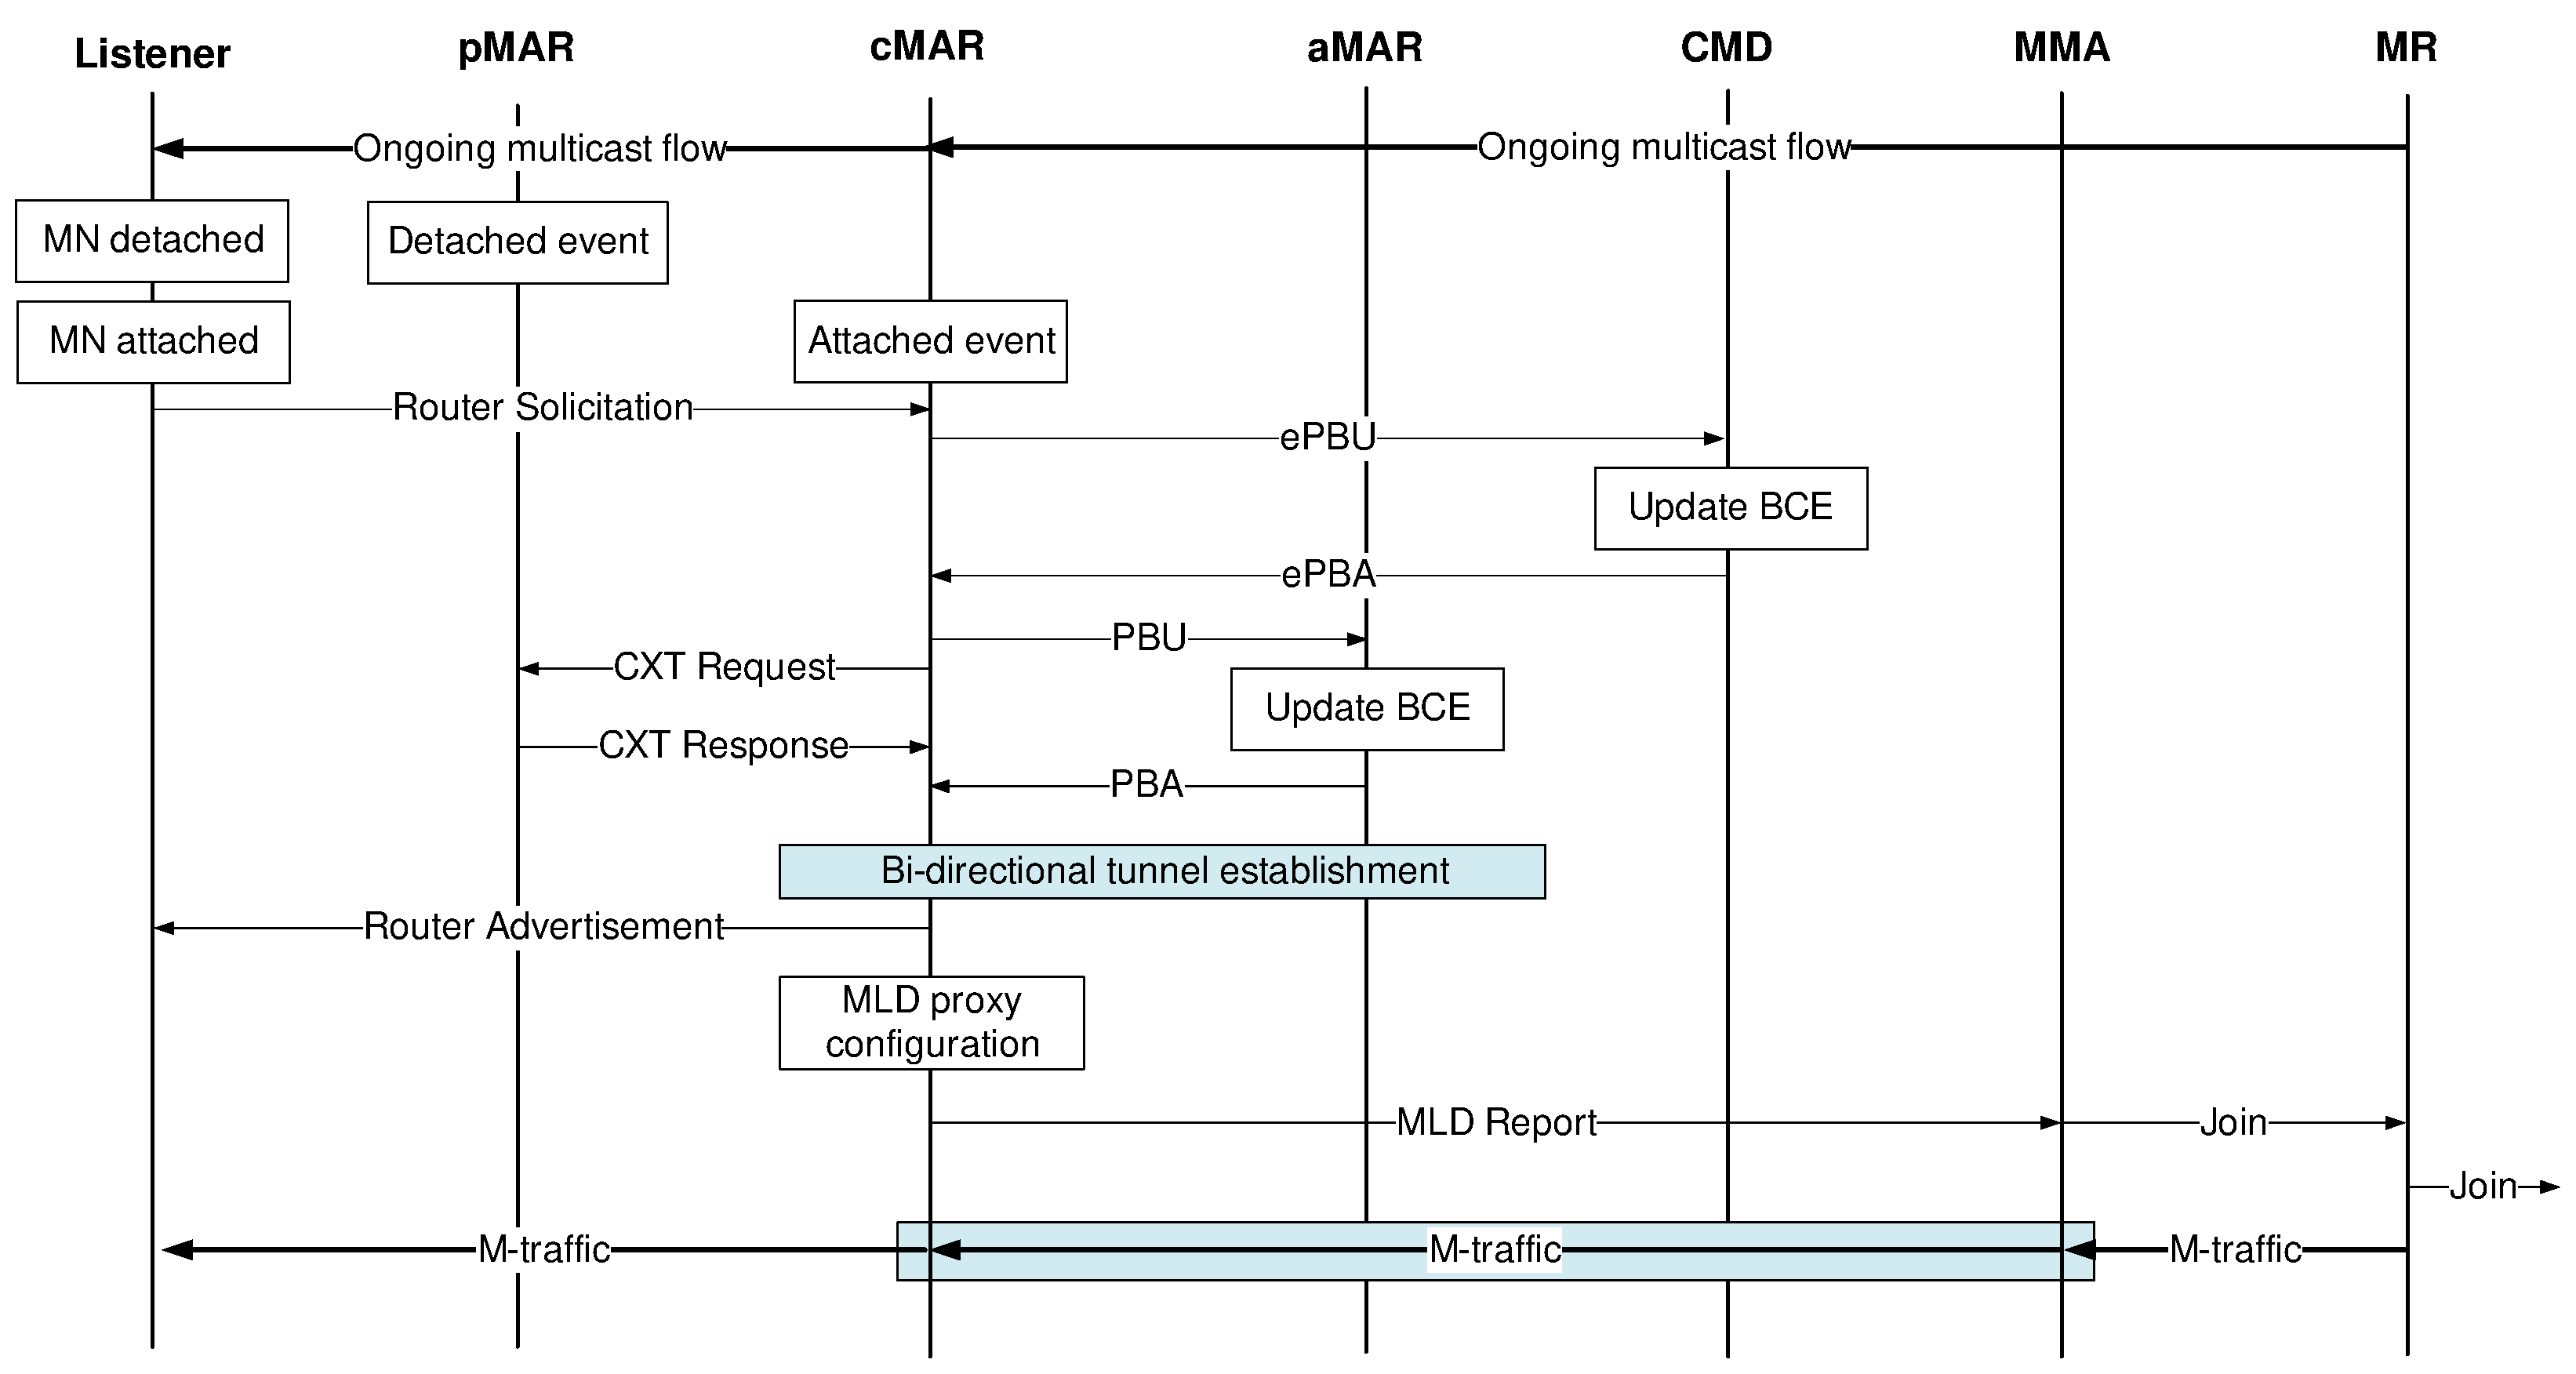
\includegraphics[width=0.90\textwidth]{./Part3/Chapter8/figures/c10_service_disruption_common.eps} 
    \caption[Signaling when a listener performs a handover in DMM.]{Signaling when a listener performs a handover in DMM.}
    \label{fig:c10_HO}
  \end{center} 
\end{figure}
To highlight these issues, this subsection considers different candidates for the MMA such as the aMAR (default mode), the pMAR, the cMAR (native subscription), or a common MMA (COMMA) which serves as only one MMA for the domain (as similar in \cite{direct_routing_mtma}). Different approaches MMA\_aMAR, MMA\_pMAR, MMA\_cMAR, and MMA\_COMMA are considered, accordingly. We also consider the impact of deploying MLD proxy with multiple upstream interfaces on the service disruption time, end-to-end delay and signaling cost. 

The signaling when a listener performs a handover in DMM is described in Fig.~\ref{fig:c10_HO}. The operations are briefly described as follows. The central mobility database (CMD), as an extended LMA, stores the MN's home network prefixes, its corresponding anchor points (aMAR) and its current location (cMAR). In case of handover, the cMAR allocates a new network prefix for this MN. The cMAR then sends a PBU to the CMD for the new prefix registration as well as retrieves the address of the anchoring MARs of the ongoing sessions. This message includes the MN\_ID, the allocated prefix at the current MAR. By looking up the BCE table, the CMD updates the entry corresponding to the MN\_ID with the current location of the MN. The CMD then replies by an extended PBA including the list of previous addresses and the corresponding prefixes. Upon receiving this message, the cMAR exchanges the PBU/PBA messages with the anchor MARs in order to update the current location of the MN. Thus, the bi-directional tunnel is established between the cMAR and each aMAR, if necessary. In parallel, the multicast context transfer messages are exchanged between the cMAR and the pMAR allowing the cMAR to obtain the active multicast subscription of the MN. For each flow, the cMAR configures an upstream interface towards the MMA (if necessary), and sends an MLD report to the MMA to join the flow. The MMA, after joining the multicast delivery tree, forwards the multicast packets to the cMAR via the tunnel between them. Finally, they reach the MN. 

\section{Quantitative Analysis} \label{c10:quantitative_analysis}
This section presents the quantitative analysis of different approaches regarding different metrics such as multicast service disruption, end-to-end delay, signaling cost and packet loss. 

\subsection{Network Model and Performance Metrics}
\subsubsection{Reference model}
\begin{figure}[tb!] 
  \begin{center} 
    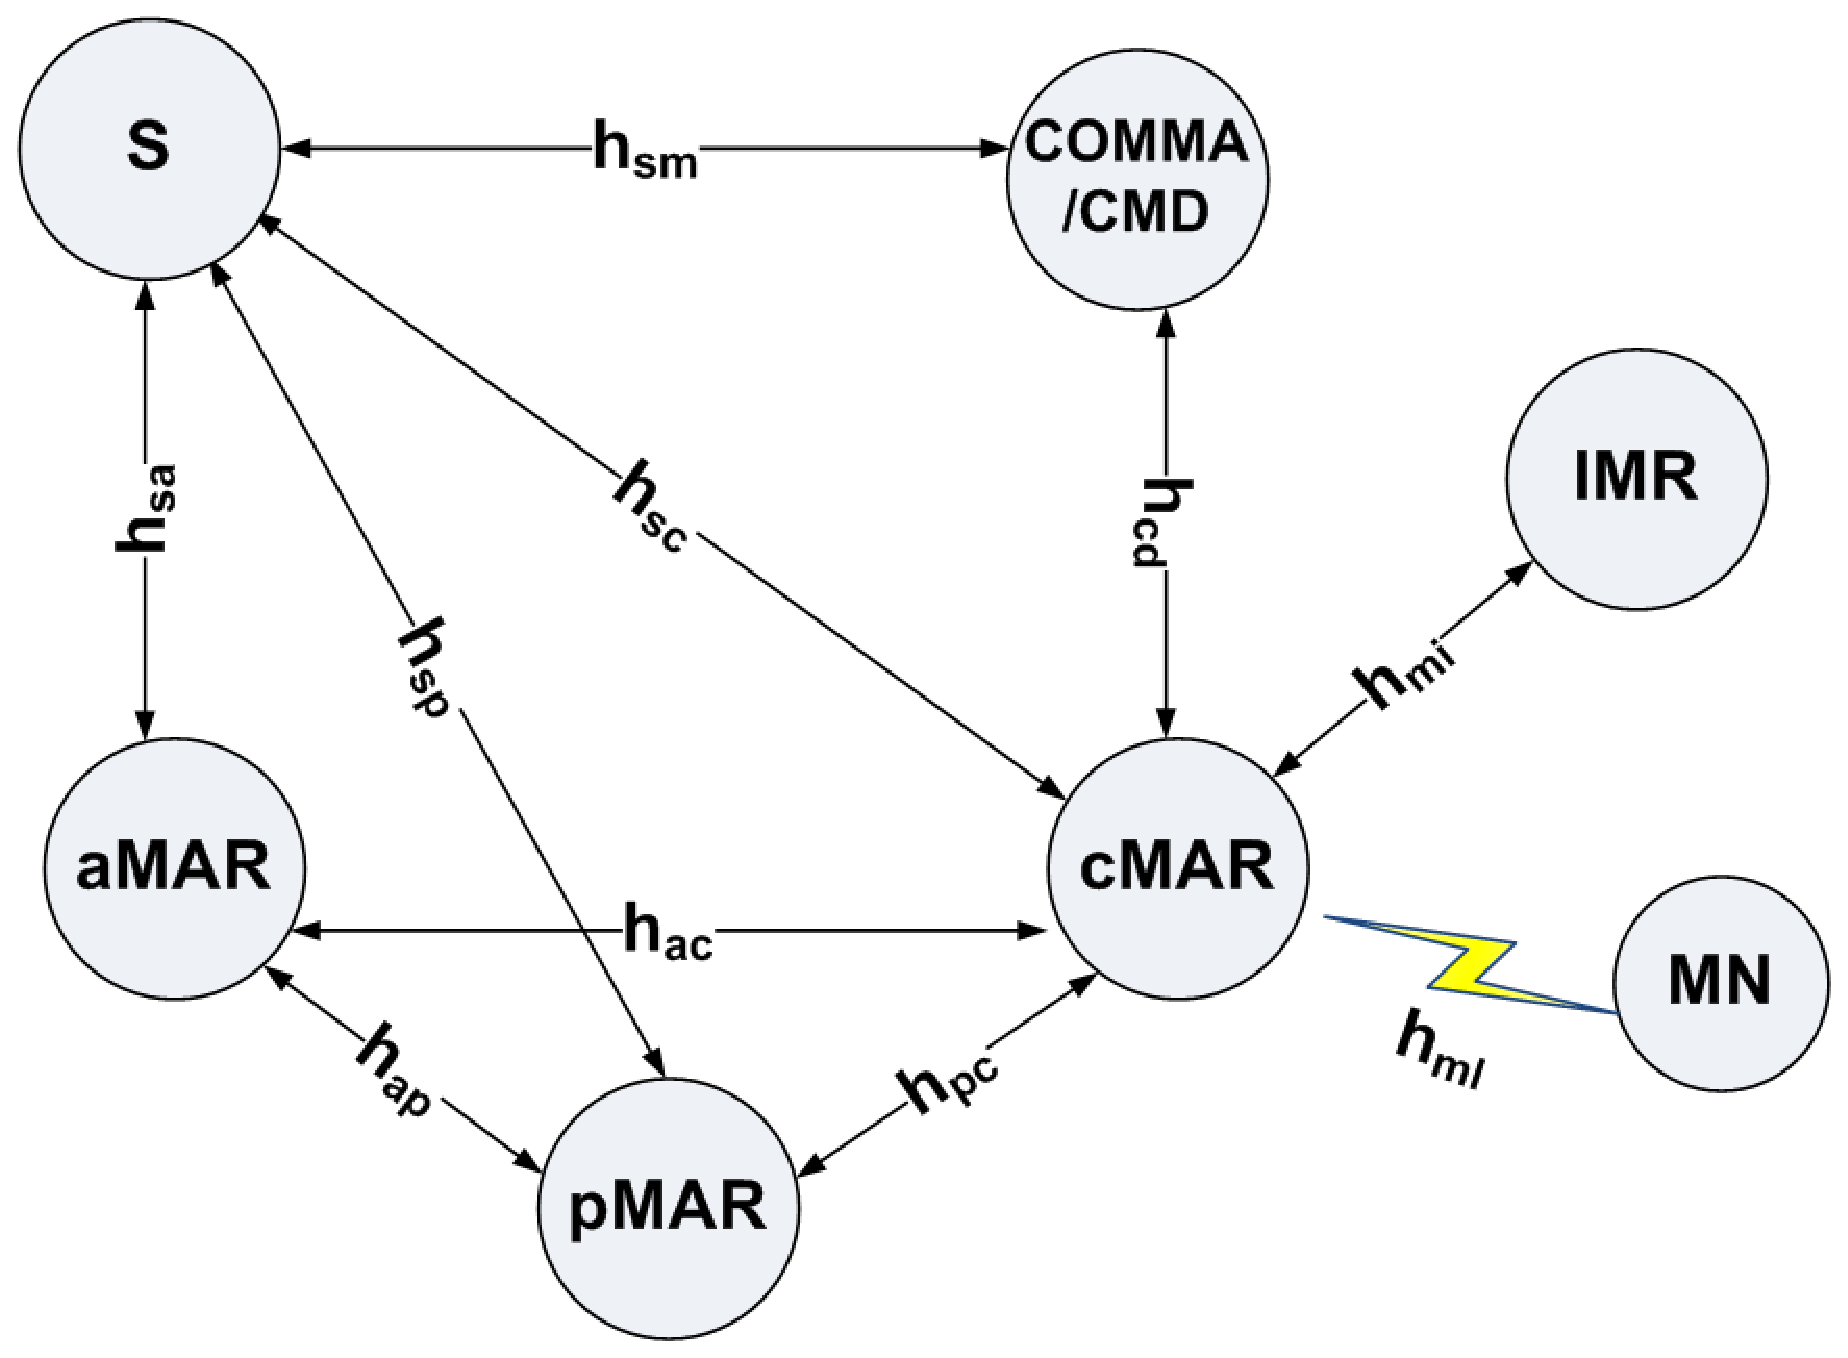
\includegraphics[width=0.55\textwidth]{./Part3/Chapter8/figures/c10_topology_analysis.eps} 
    \caption{Reference network topology.}
    \label{fig:c10_topology_analysis}
  \end{center} 
\end{figure}

Fig.~\ref{fig:c10_topology_analysis} shows a reference topology for the performance analysis. The hop-count distances between the entities are defined as follows:
\setlength \abovedisplayskip{-1pt}
\vspace{-0.1in}
\begin{itemize}
\itemsep 0.07em
\item $h_{ac}$: the average number of hops between the aMAR and the cMAR.
\item $h_{ap}$: the average number of hops between the aMAR and the pMAR.
\item $h_{pc}$: the average number of hops between the pMAR and the cMAR.
\item $h_{cd}$: the average number of hops between the MAR and the CMD/COMMA.
\item $h_{ml}$: the average number of hops between the MAR and the listener (MN), it is assumed to be one (wireless link).
\item $h_{sa}$: the average number of hops between the source S and the aMAR.
\item $h_{sp}$: the average number of hops between the source S and the pMAR.
\item $h_{sc}$: the average number of hops between the source S and the cMAR.
\item $h_{sm}$: the average number of hops between the source S and the COMMA.
\item $h_{mr}$: the average number of hops between the MAR and its upstream MR, it is assumed to be one. 
\item $h_{mi}$: the average number of hops between the cMAR and the intersection MR (IMR) which already has a multicast forwarding state for the group.
\end{itemize}

We then define the network scale $\psi$ which is the ratio between the number of hops between two adjacent MARs ($h_{mm}$) and the number of hops between the MAR and the CMD ($h_{cd}$).\\
\begin{equation}
\psi = \frac{h_{mm}}{h_{cd}}.
\end{equation} 
Typically, the average number of hops between two adjacent MARs is less than that between an MAR and a centralized entity. That means $\psi \leq 1$. In this chapter, we will investigate the impact of the network scale on the performance metrics by varying the value of $\psi$ over a range [0,1] (by varying $h_{mm}$ while fixing the value of $h_{cd}$). 
\subsubsection{Messages Related to the Performance Analysis}
As described in Fig.~\ref{fig:c10_HO}, various messages are used in our analysis. For a sake of simplicity, we suppose that there is only one ongoing flow. The following message sizes in bytes are considered in our analysis:
\begin{itemize}
\item $L_{RS}$: It is the size of the Router Solicitation (RS) message, which is 52.
\item $L_{RA}$: It is the size of the Router Advertisement (RA) message, which is 80.
\item $L_{PBU}$: It is the size of the PBU message, which is 84.
\item $L_{PBA}$: It is the size of the PBA message, which is 92.
\item $L_{ePBU}$: It is the size of the extended PBU message, which is 84.
\item $L_{ePBA}$: It is the size of the extended PBA message, which is 128.
\item $L_{M-Req}$: It is the size of the multicast context transfer request message, which is 86.
\item $L_{M-Res}$: It is the size of the multicast context transfer response message, which is 104.
\item $L_{C-Req}$: It is the size of the channel configuration request message, which is 92.
\item $L_{C-Res}$: It is the size of the channel configuration response message, which is 112. 
\item $L_{MLD-R}$: It is the size of the MLD Report message, which is 96.
\item $L_{Join}$: It is the size of the PIM Join message, which is 110.
\item $L_{MP}$: It is the size of the multicast packet, which is 200.
\item $L_{T}$: It is the size of the tunneling header, which 40.  
\end{itemize}

It is noted that the values of $L_{PBU}$,  $L_{PBA}$, $L_{ePBU}$, $L_{ePBA}$, $L_{M-Req}$ $L_{M-Res}$, $L_{C-Req}$ and $L_{C-Res}$ are taken from the real implementation of PMIPv6 \cite{oai_pmip} and the multicast context transfer function \cite{d4.4}, while the others are from \cite{HO_comparison_Lee,DMM_analysis_Hassan}.  

\subsubsection{Delay Model}
As described in Chapter \ref{ch:performance_evaluation}, we adopt the packet transmission delay model in \cite{packet_transmission_delay} in which the packet transmission consists of the transmission time and the propagation time.  
Thus, the transmission delay of a wired link can be calculated as\\
\begin{equation}
d_{wd}(l,h) = h (\dfrac{l}{BW_{wd}} + D_{wd}),
\end{equation}
where h is the hop-count distances between two nodes, l is the length of the packet, $BW_{wd}$ is the bandwidth of wired link and $D_{wd}$ is the wired link latency. 

Unlike the wired transmission which can be considered as reliable, the wireless link is unreliable. The wireless transmission delay is therefore calculated as \cite{packet_transmission_delay}\\
\begin{equation}
d_{wl}(l) = \dfrac{1}{1-q} (\dfrac{l}{BW_{wl}} + D_{wl}),
\end{equation} 
where q is the probability of wireless link failure, $BW_{wl}$ is the bandwidth of wireless link and $D_{wl}$ is the wireless link latency.  

\subsubsection{Mobility Model}
In this chapter, we consider the case where the MN always moves from MAR to MAR as if they were linearly deployed (the user is moving further away from the first attached MAR and never attaches back to a previously visited MAR). It represents the worst-case scenario. Thus, we have $h_{ac}$ = $h_{ap}$ + $h_{pc}$.
Let $N_{mar}$ denote the average number of MARs involved in the data traffic forwarding to/from an MN. In our context, $N_{mar}$ is also the number of handovers. We therefore obtain \\
\begin{equation}
h_{ac} = N_{mar} h_{mm},
\end{equation} 
\begin{equation}
h_{pc} = h_{mm}.
\end{equation}

In our analysis, the low value of $N_{mar}$ represents the low mobility node and the short-lived flow scenarios. The higher value of $N_{mar}$ corresponds to the high mobility and long-lived flow scenarios.   

\subsection{Analytical Modeling}
This subsection develops an analytical model regarding the following performance metrics: the multicast service disruption time ($SD(.)$), representing the period when the listener cannot receive the multicast packet; the end-to-end delay ($E2E(.)$) - the transmission time from source to listener; the signaling cost ($SC(.)$) - the cost for supporting multicast handover; the packet delivery cost ($DC(.)$) - the cost to deliver multicast packets from the source to the listener; the packet tunneling cost ($TC(.)$) - the tunnel overhead;  and packet loss ($\varphi_{p}$) - the number of lost packets during handover. In the performance analysis, we consider the normal case and the case where the MLD proxy supports the multiple upstream interfaces capability. We then highlight the impacts and benefits of using multiple upstream interfaces on these metrics. 

\subsubsection{Multicast Service Disruption Time Analysis}
The multicast service disruption time ($SD(.)$) is defined as a period when a multicast listener is unable to receive the multicast packets. 
Assuming that the delay associated with the processing of the messages in the network entities (e.g., time for PBU processing and updating binding cache in MAR) is included in the total value of each variable. Then the service disruption time is (see Fig.~\ref{fig:c10_HO}) \\
\small
\begin{equation}
SD(.) = T_{L2} + d_{wl}(L_{RS}) +T_{CMD} + max \{ T_{LU}, T_{CXT}\}  +max \{d_{wl}(L_{MP}), T_{M}{(.)} + d_{wl}(L_{MP})\},
\label{eq:sd}
\end{equation}
\normalsize
where $T_{L2}$ is the L2 handover duration, $T_{CMD}$ is the time needed to get the address of the anchor/previous MAR from the CMD, $T_{LU}$ is the location update time (at the aMAR), $T_{CXT}$ is the time for the context transfer messages exchanged, $T_{M} (.)$ is the time needed for the cMAR to join and get the first multicast packet after handovers. 

In Eq.~(\ref{eq:sd}), except $T_{M}{(.)}$, the other components are the same in different approaches, and given by\\
\begin{equation}
T_{CMD} = d_{wd}(L_{ePBU},h_{cd}) + d_{wd}(L_{ePBA},h_{cd}),
\end{equation}
\begin{equation}
T_{LU} = d_{wd}(L_{PBA}, h_{ac}) + d_{wd}(L_{PBU}, h_{ac}),
\end{equation}
\begin{equation}
T_{CXT} = d_{wd}(L_{M-Req},h_{pc}) +d_{wd}(L_{M-Res},h_{pc}).
\end{equation}

In (\ref{eq:sd}), $T_{M}^{(.)}$ represents the time needed for the cMAR to join and get the first multicast packet. In case of MMA\_cMAR, the cMAR has to get the multicast traffic from the IMR which already has a multicast forwarding state for this group. Thus, \\
\small
\[ T_{M}(cMAR) = \left\{ 
 \begin{array}{l l}
   \overline{w}_{mr} \quad \small \text{if } h_{mi} =0,  \\
   (h_{mi} +1) \overline{w}_{mr}+d_{wd}(L_{MLD-R}) + d_{wd}(L_{MP}) +  d_{wd}(L_{Join},h_{mi}-1) \\+d_{wd}(L_{MP},h_{mi}-1)   \quad \small \text{if }h_{mi} \geq 1. 
 \end{array} \right.\] 
\normalsize 
where $\overline{w}_{mr}$ is the delay time in which an MR (and an MLD proxy) needs to join a multicast flow at each router (proxy) in the internet \cite{MPDSR}. 

In case of MMA\_pMAR, the pMAR already had the multicast state for this flow. We have \\
\begin{equation}
T_{M}(pMAR) = 2\overline{w}_{mr} +d_{wd}(L_{MLD-R}+L_{T},h_{pc})+d_{wd}(L_{MP} +L_{T},h_{pc}).
\end{equation}

In case of MMA\_aMAR, there are two possibilities: the normal case (case 1, without deploying the multiple upstream interfaces, thus, corresponding to the default mode), and the case where MLD proxy with multiple upstream interfaces is deployed at MARs. In the latter case, in the worst situation, the aMAR needs to join the multicast channel, leading to an extra delay. It happens, for example, in case the multicast traffic was received from the multicast infrastructure in the pMAR and the aMAR has left the channel. Let $p_{a}$ denote the probability that this situation happens. As a result, $T_{M}(.)$ is calculated as \\
\begin{equation}
T_{M}(aMAR) =(1-p_{a}) T_{M}(aMAR-c1)  +p_{a} T_{M}(aMAR-wc),
\end{equation}
where
\begin{equation}
T_{M}(aMAR-c1) =2\overline{w}_{mr} +d_{wd}(L_{MLD-R}+L_{T},h_{ac})+d_{wd}(L_{MP} +L_{T},h_{ac}),
\end{equation}
\small
\[T_{M}(aMAR-wc)  = \left\{ 
 \begin{array}{l l}
   T_{M}(aMAR-c1)  \quad \small \text{if } h_{mi} =0,  \\
    T_{M}(aMAR-c1)+ d_{wd}(L_{MLD-R})+ d_{wd}(L_{MP})  + d_{wd}(L_{Join},h_{mi}-1) \\+ (h_{mi}+1)  \overline{w}_{mr} +d_{wd}(L_{MP},h_{mi}-1)  \quad \small \text{if }h_{mi} \geq 1. 
 \end{array} \right.\] 
\normalsize 

It is noted that $T_{M}(aMAR-c1)$ represents the multicast service disruption time in the default mode, when $T_{M}(aMAR)$ shows the impact of using MLD proxy with multiple upstream interfaces on the service disruption time. As a result, $SD(aMAR)$ can be considered as a trade-off between the service disruption and the tunnel convergence problem.  

In case of MMA\_COMMA, we have \\
\begin{equation}
T_{M}(COMMA)= 2\overline{w}_{mr}+  d_{wd}(L_{MLD-R}+L_{T}, h_{cd}) + d_{wd}(L_{MP}+L_{T}, h_{cd}).
\end{equation}
\subsubsection{End-to-End Delay}
End-to-end delay ($E2E(.)$) is the packet transmission delay from the source to the listener. In the MMA\_cMAR, the cMAR receives the multicast traffic directly from the multicast infrastructure. Hence, the end-to-end delay is given by\\
\begin{equation}
E2E(cMAR) = d_{wd}(L_{MP},h_{sc}) + d_{wl}(L_{MP}).
\end{equation}

In the MMA\_aMAR, the multicast packet is routed from the source to the cMAR via the aMAR, representing the default multicast mode. We have \\
\begin{equation}
E2E(aMAR) = d_{wd}(L_{MP},h_{sa}) + d_{wd}(L_{MP}+L_{T},h_{ac}) + d_{wl}(L_{MP}).
\end{equation}

In case of MMA\_pMAR, the MAR always receives the multicast traffic from its pMAR in the normal case. Therefore, the end-to-end delay is given as follows \\
\begin{equation}
E2E(pMAR-c1)= d_{wd}(L_{MP},h_{sa}) + d_{wd}(L_{MP} +L_{T},h_{ap}) + d_{wd}(L_{MP} + L_{T},h_{pc})  + d_{wl}(L_{MP}).
\end{equation}

In case of using multiple upstream interfaces, we suppose that $p_{p}$ is the probability that the MAR gets multicast traffic from its upstream interfaces. Thus, $1-p_{p}$ is the probability the MAR gets the multicast traffic from its pMAR. The end-to-end delay in case of MMA\_pMAR is therefore given by
\begin{multline}
E2E(pMAR)=   d_{wl}(L_{MP}) + [d_{wd}(L_{MP},h_{sa})+ N_{mar} d_{wd}(L_{MP} +L_{T},h_{mm})] p_{p}^{N_{mar}-1} \\+ \sum_{i=1}^{N_{mar}-1} [d_{wd}(L_{MP},h_{i})+ (N_{mar}-i) d_{wd}(L_{MP} +L_{T},h_{mm})] p_{p}^{N_{mar}-i-1} (1-p_{p}),
\end{multline}
where $h_{i}$ is the hop-count distances from the source to the $i^{th}$ MAR in the moving path of the MN (from the aMAR to the cMAR), for example, $ h_{N_{mar}-1} = h_{sp}$ .  

Considering the MMA\_COMMA, the end-to-end delay is expressed as\\
\begin{equation}
E2E(COMMA) = d_{wd}(L_{MP},h_{sm})  + d_{wd}(L_{MP}+L_{T},h_{cd}) + d_{wl}(L_{MP}).
\end{equation}

\subsubsection{Cost Analysis}
In this subsection, the signaling cost ($SC(.)$), the packet delivery cost ($PC(.)$) and the tunneling cost ($TC(.)$) are investigated. The signaling cost (per handover) is the signaling overhead for supporting the handover including multicast-related procedures. It can be calculated as \\
\begin{equation}
SC(.) =SC_{LU} + SC_{M}(.),
\end{equation}
where $SC_{LU}$, $SC_{M}(.)$ is the signaling cost for the location update and the multicast-related procedures, respectively. As mentioned in Chapter \ref{ch:performance_evaluation}, the signaling message delivery cost is calculated as the product of the message size, the hop distance and the unit transmission cost in a wired/wireless link ($\alpha$ for the wired and $\beta$ for the wireless link). $SC_{LU}$ is therefore given by\\
\begin{equation}
SC_{LU} = \beta (L_{RS} + L_{RA}) + \alpha (L_{ePBU}  h_{cd} + L_{ePBA} h_{cd})  + \alpha (L_{PBU}  h_{ac} + L_{PBA} h_{ac}).
\end{equation}
$SC_{M}(.)$ is expressed as\\
\begin{equation}
SC_{M}(cMAR) = \alpha  (L_{M-Req}  h_{pc} + L_{M-Res} h_{pc} + L_{MLD-R} + L_{Join} h_{mi}).
\end{equation}
\begin{equation}
SC_{M}(pMAR) = \alpha (L_{M-Req}  h_{pc} + L_{M-Res} h_{pc} + L_{MLD-R} h_{pc}).
\end{equation}
\begin{equation}
SC_{M}(aMAR) =(1-p_{a}) SC_{M}(aMAR-c1)  + p_{a} SC_{M}(aMAR-wc),
\end{equation}
where 
\begin{equation}
SC_{M}(aMAR-c1) = \alpha (L_{M-Req}  h_{pc} + L_{M-Res} h_{pc} +L_{MLD-R} h_{ac}),
\end{equation}
\begin{equation}
SC_{M}(aMAR-wc) = \alpha (L_{M-Req}  h_{pc} + L_{M-Res} h_{pc}  + L_{MLD-R} h_{ac}+L_{MRD-R} +L_{Join} h_{mi}).
\end{equation}

\begin{equation}
SC_{M}(COMMA) = \alpha (L_{M-Req}  h_{pc} + L_{M-Res} h_{pc}  + L_{MLD-R} h_{cd}).
\end{equation}

The packet delivery cost represents the cost of delivering multicast packets to the MN per unit of time. Let $S_{c}$, $\lambda_{p}$ denote the average session length at the cMAR and the packet arrival rate, respectively. Again, the packet delivery cost in the MMA\_aMAR corresponds to the default multicast mode. The packet delivery cost is expressed as\\
\begin{equation}
PC(cMAR) = S_{c} \lambda_{p} (\alpha L_{MP} h_{sc}  + \beta L_{MP}).
\end{equation}
\begin{equation}
PC(aMAR) = S_{c} \lambda_{p} [\alpha L_{MP} h_{sa} + \alpha (L_{MP} + L_{T}) h_{ac}  + \beta L_{MP}].
\end{equation}

In case of MMA\_pMAR, in the normal case, the MAR always receives the multicast traffic from its pMAR. Thus, the packet delivery cost is given as follows \\
\begin{equation}
PC(pMAR-c1)=  S_{c} \lambda_{p} [\alpha  L_{MP} h_{sa} +  \alpha  (L_{MP} + L_{T}) ( h_{ap} + h_{pc}) + \beta L_{MP}].
\end{equation}
Using the multiple upstream interfaces, the packet delivery cost is calculated as
\begin{multline}
PC(pMAR)= S_{c} \lambda_{p}  \beta L_{MP} +  S_{c} \lambda_{p} [\alpha L_{MP} h_{sa}+ \alpha N_{mar}  (L_{MP} +L_{T}) h_{mm}] p_{p}^{N_{mar}-1} \\+ S_{c} \lambda_{p} \sum_{i=1}^{N_{mar}-1} [\alpha L_{MP} h_{i}+ \alpha  (N_{mar}-i) (L_{MP} +L_{T}) h_{mm}] p_{p}^{N_{mar}-i-1} (1-p_{p}).
\end{multline}

In case of MMA\_COMMA, the packet delivery cost is\\
\begin{equation}
PC(COMMA) = S_{c} \lambda_{p} [\alpha L_{MP} h_{sm} + \alpha (L_{MP} + L_{T}) h_{cd}  + \beta L_{MP}].
\end{equation}

Regarding the packet tunneling cost, it is defined as the additional cost from the tunneling overhead. In MMA\_cMAR, the multicast traffic is received directly from the multicast infrastructure, thus, there is no tunneling cost. On the contrary, in MMA\_aMAR, MMA\_pMAR, and MMA\_COMMA the traffic is routed via the tunnel aMAR-cMAR, pMAR-cMAR, and cMAR-COMMA, respectively. Note that the tunneling cost in the MMA\_aMAR corresponds to the default multicast mode. The tunneling cost is therefore computed as\\ 
\begin{equation}
TC(cMAR) = 0. 
\end{equation}
\begin{equation}
TC(aMAR) = \alpha  S_{c} \lambda_{p} (L_{MP} + L_{T}) h_{ac}. 
\end{equation}
\begin{equation}
TC(pMAR)=  \alpha  S_{c} \lambda_{p} (L_{MP} + L_{T}) h_{mm}  \sum_{i=0}^{N_{mar-1}} (N_{mar}-i)p_{p}^{N_{mar}-i-1} (1-\theta p_{p}).
\end{equation}
where 
\[\theta  = \left\{ 
 \begin{array}{l l}
   0 \quad \small \text{if } i =0,  \\
    1  \quad \small \text{if } i \geq 1. 
 \end{array} \right.\] 

\begin{equation}
TC(COMMA) = \alpha  S_{c} \lambda_{p} (L_{MP} + L_{T}) h_{cd}. 
\end{equation}

The signaling cost in general is an important factor which influences the scalability of the networks. However, as data and control plane are no longer coupled, in case where a huge amount of traffic is generated in the network, the packet delivery cost and tunneling cost play more important role.  
 
\subsubsection{Packet Loss}
During the handover, packets may be lost. The number of lost packets is proportional to the service disruption time and the packet arrival rate. As a result, the number of lost packets is given by\\
\begin{equation}
\varphi_{p}(.)= \lambda_{p} SD(.).
\end{equation}

\normalsize
\subsection{Numerical Results}
This subsection presents the numerical results based on the analysis given in the previous one. The default parameter values for the analysis are introduced in Table \ref{tap:c10_parameters}, in which some parameters are taken from \cite{dsrm}\cite{d4.4}. It is worth noting that the $SD (aMAR-c1)$, $E2E(aMAR)$, $SC(aMAR-c1)$, $PC(aMAR)$, and $TC(aMAR)$ correspond to the default mode in our analysis. \\

\begin{table}[ht]
\small
\caption{Parameters for the performance analysis.}
\label{tap:c10_parameters}
\centering
\begin{tabular}{|c |c |c |c |c |c |}
\hline
\textbf{Parameter} & \textbf{Value} & \textbf{Parameter} & \textbf{Value} & \textbf{Parameter} & \textbf{Value}  \\
\hline
$T_{L2}$ & 50ms & $BW_{wd}$  &  100Mbps & $BW_{wl}$  & 11 Mbps\\
\hline
  $D_{wd}$& 2ms  & $D_{wl}$ & 10ms & $q$& 0.35  \\
\hline
$\overline{w}_{mr}$&  10 ms  & $h_{mm}$ & 3 hops & $h_{cd}$&  12 hops  \\
\hline
$h_{mi}$& 2 hops  & $h_{sa}$& 16 hops  & $h_{sp}$&  16 hops   \\
\hline
 $h_{sc}$  & 16 hops   & $h_{sm}$&  16 hops &$S_{c} $&  60 s  \\
\hline
$\lambda_{p}$& 10 packets/s  & $\alpha$&  1 & $\beta $&  5  \\
\hline
$p_{p}$& 0.9  & $p_{a}$&  0.5 & & \\
\hline
\end{tabular}
\end{table}
\normalsize

\subsubsection{Multicast Service Disruption Time}
\begin{figure}[!h]
\centering
\subfloat[]{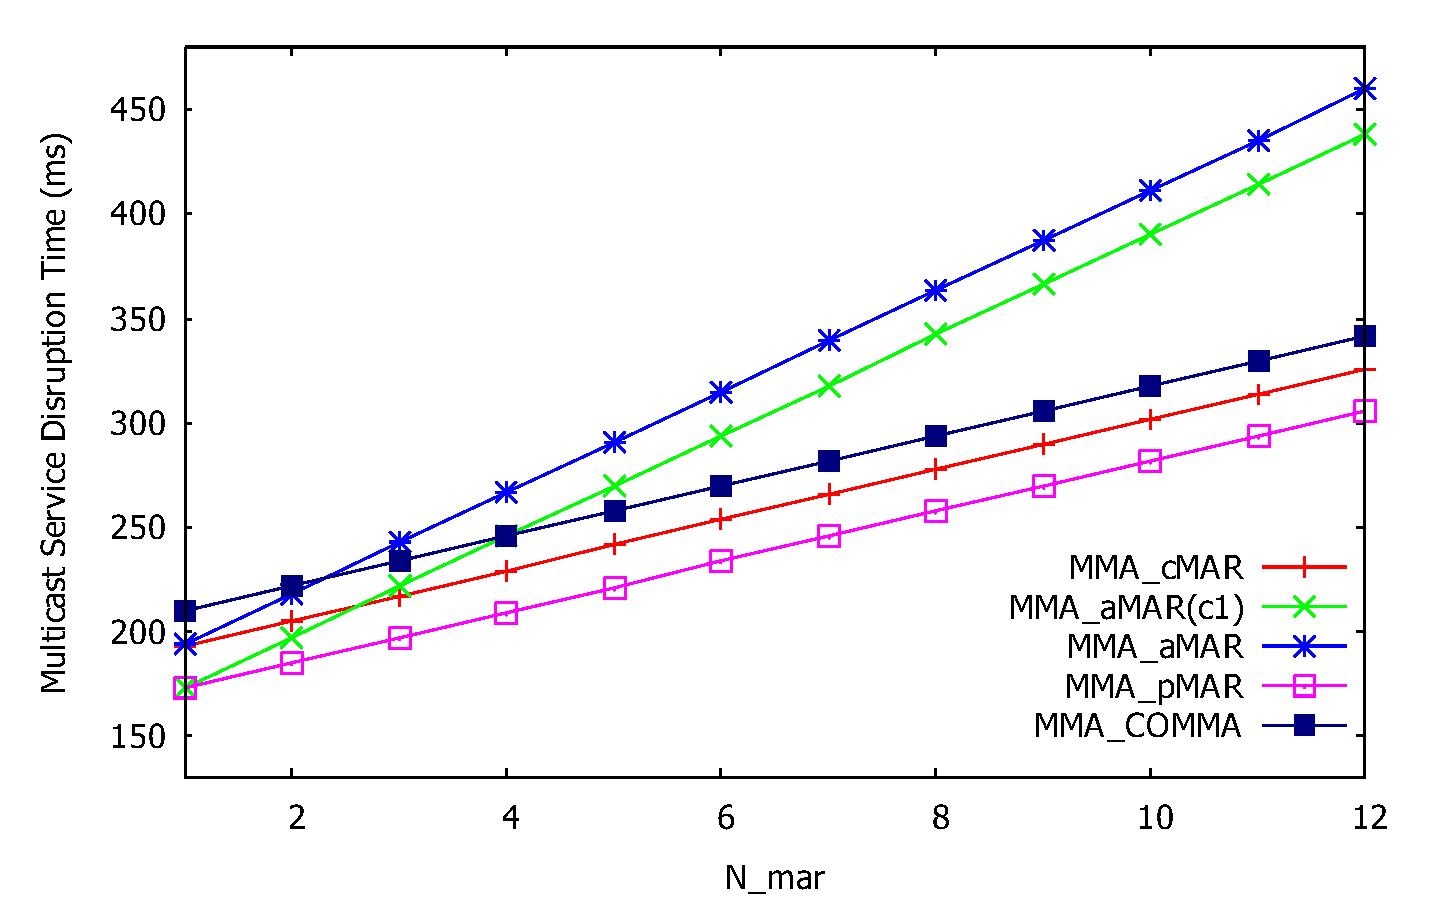
\includegraphics[scale=0.28]{./Part3/Chapter8/figures/c10_sd_n_mar.eps} \label{fig:c10_sd_n_mar}}
\subfloat[]{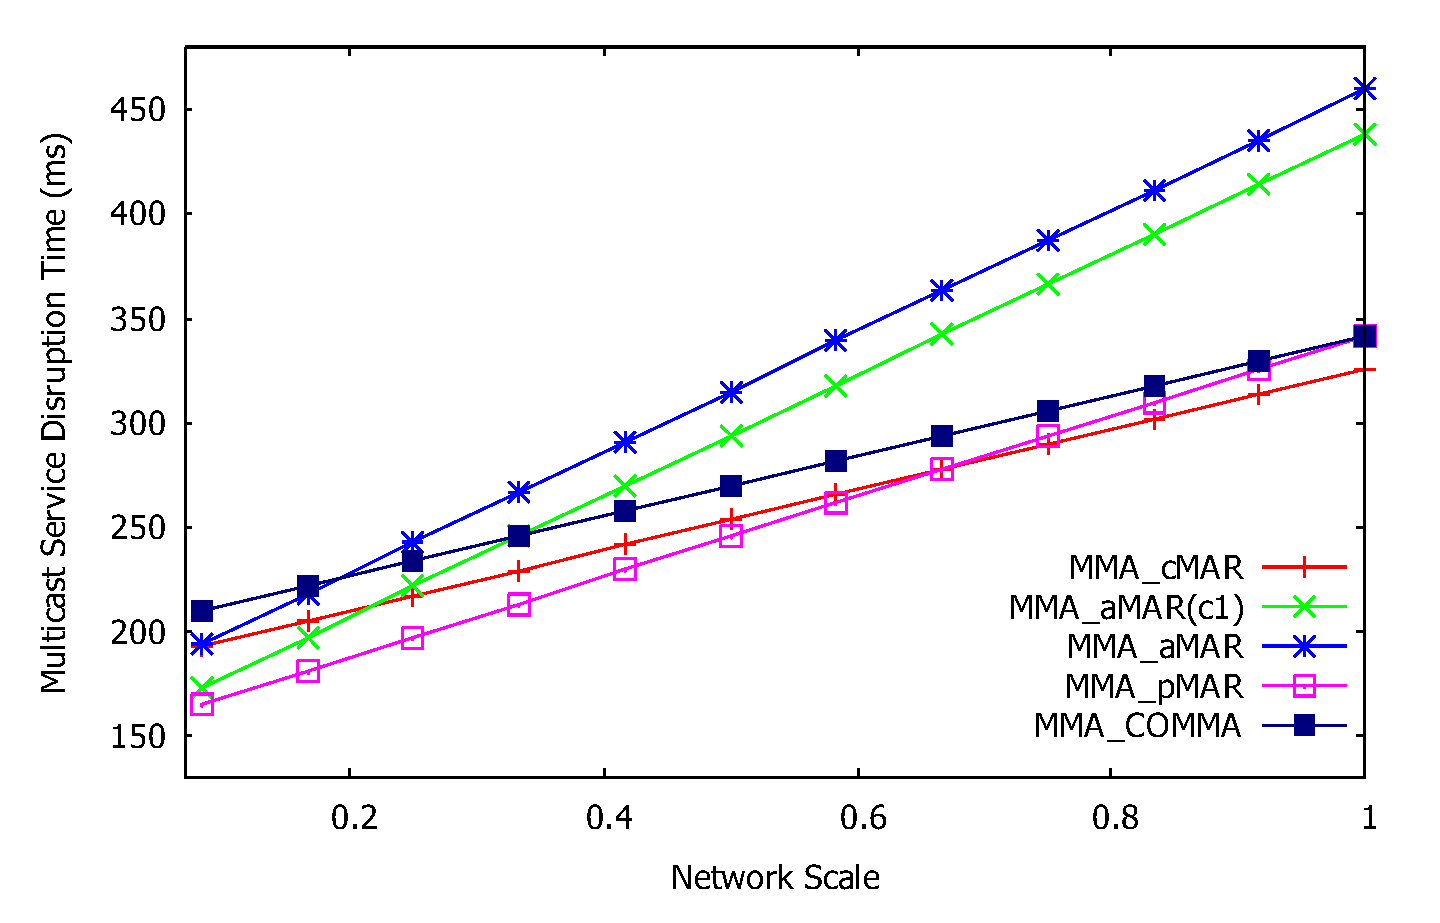
\includegraphics[scale=0.28]{./Part3/Chapter8/figures/c10_scale.eps}\label{fig:c10_scale}}\,
\subfloat[]{\includegraphics[scale=0.28]{./Part3/Chapter8/figures/c10_h_mi.eps}\label{fig:c10_h_mi}}
\caption[Multicast service disruption time.]{Multicast service disruption time as a function of: (a) $N_{mar}$, (b) $\psi$, (c) $h_{mi}$.}
\label{fig:c10_sd}
\end{figure}

Fig.~\ref{fig:c10_sd_n_mar} shows the multicast service disruption time when $N_{mar}$ is varied over a range from 1 to 12. It appears clearly that the MMA\_pMAR approach gives a better performance than the others (lower is better). The service disruption time in the MMA\_cMAR is slightly greater than that in the MMA\_pMAR since the value of $h_{mi}$ in this case is quite small (2 hops). When $N_{mar}$ is small (less than 5), all approaches satisfy the requirement in terms of service disruption for real-time services (lower than 300ms). When $N_{mar}$ is relatively big, the service disruption in case of MMA\_aMAR is significantly increased. We also investigate the impact of the network scale ($\psi$) on the service disruption time. In this case, $N_{mar}$ is set to a value of 3. In general, the impact of $\psi$ is similar to that of $N_{mar}$. Especially, Fig. \ref{fig:c10_scale} shows that there is an area where the MMA\_cMAR outperforms the MMA\_pMAR (when the network scale is larger than 0.62).

Fig.~\ref{fig:c10_h_mi} shows the multicast service disruption time when $h_{mi}$ is varied over a range from 0 to 10 hops. A small value of $h_{mi}$ indicates a high listener density scenario while a high value of $h_{mi}$ represents a low listener density scenario. The service disruption in the MMA\_pMAR is lower than that in the others (except when $h_{mi}=0$ indicating the case where the multicast traffic is already available at the cMAR's upstream MR). As the value of $h_{mi}$ increases, the service disruption time in the MMA\_pMAR, MMA\_aMAR (c1) and MMA\_COMMA is kept constant while that in the other cases is significantly increased. As a result, the difference between the approaches is increased. It comes from the fact that the multicast traffic is already available at the pMAR, aMAR, and COMMA in case of MMA\_pMAR, MMA\_aMAR(c1) and MMA\_COMMA, respectively. Additionally, the service disruption time in the MMA\_cMAR strongly depends on the value of $h_{mi}$. In other words, it cannot be guaranteed in the MMA\_cMAR approach. Also, in the MMA\_aMAR, it increases significantly compared to that in the MMA\_aMAR (c1) as a consequence of using multiple upstream interfaces in DMM. 

\begin{figure}[h!]
\centering
\subfloat[]{\includegraphics[width=0.50\textwidth]{./Part3/Chapter8/figures/c10_e2e_n_mar.eps} \label{fig:c10_e2e_n_mar}}
\subfloat[]{\includegraphics[width=0.50\textwidth]{./Part3/Chapter8/figures/c10_e2e_scale.eps}\label{fig:c10_e2e_scale}}\,
\subfloat[]{\includegraphics[width=0.50\textwidth]{./Part3/Chapter8/figures/c10_e2e_h_sc.eps}\label{fig:c10_e2e_h_sc}}
\caption[End-to-end delay.]{End-to-end delay as a function of: (a) $N_{mar}$, (b) $\psi$, (c) $h_{sc}$.}
\label{fig:c10_e2e}
\end{figure}
In conclusion, MMA\_pMAR is generally well suited for service interruption sensitive services. Moreover, the service disruption in the MMA\_aMAR is always greater than that in the MMA\_aMAR (c1). Thus, the increasing of service disruption time, which is caused by enabling the multiple upstream interfaces for the MLD proxy, can be considered as a trade-off between the service disruption time and the tunnel convergence problem. 

\subsubsection{End-to-End delay}
Now we investigate the impact of $N_{mar}$ on the end-to-end delay. Fig.~\ref{fig:c10_e2e_n_mar} shows the plot for the end-to-end delay versus the number of handover $N_{mar}$. As $N_{mar}$ increases ($h_{ac}$ increases) the end-to-end delay in case of MMA\_aMAR and MMA\_pMAR rapidly increases, while that in MMA\_cMAR and MMA\_COMMA is kept constant. Note that the end-to-end delay in MMA\_cMAR is kept below the value 50 ms. That means the MMA\_cMAR satisfies the strict requirement in terms of end-to-end delay (for real-time gaming \cite{e2e_requirement}). The delay in MMA\_pMAR(c1) is greater than that in MMA\_pMAR as a result of using the multiple upstream interfaces. As can be seen in Fig.~\ref{fig:c10_e2e_scale}, in general, the network scale has a similar impact on the end-to-end delay as $N_{mar}$. The major difference is that the increasing line of MMA\_pMAR in Fig.~\ref{fig:c10_e2e_scale} is faster than that in Fig.~\ref{fig:c10_e2e_n_mar}.

Then, $N_{mar}$ is set to a value of 6 (corresponding to the medium/long-lived and medium/high mobility scenario) while the value of $h_{sc}$ is varied. At this stage, we suppose that $h_{sa}$ + $h_{sc}$ is a fixed value, for example, 18 hops and $h_{sp}$ = $h_{sc}$. This scenario is used to illustrate the case where the source is extremely close to the aMAR (right-side of Fig.~\ref{fig:c10_e2e_h_sc}) or extremely close to the cMAR (left side of Fig.~\ref{fig:c10_e2e_h_sc}). As can be observed in Fig.~\ref{fig:c10_e2e_h_sc}, even when the source is very close to the aMAR ($h_{sa}$=2, $h_{sc}$=16), the MMA\_cMAR approach gives a better performance in terms of end-to-end delay than the others (lower is better). Thus, the impact of the mobility tunnel (cMAR-aMAR and cMAR-pMAR) on the end-to-end delay is obvious. In conclusion, the cMAR is generally well suited for the delay-sensitive flows. 
\begin{figure}[h!]
\centering
\subfloat[]{\includegraphics[width=0.50\textwidth]{./Part3/Chapter8/figures/c10_sc_n_mar.eps} \label{fig:c10_sc_n_mar}}
\subfloat[]{\includegraphics[width=0.50\textwidth]{./Part3/Chapter8/figures/c10_sc_scale.eps}\label{fig:c10_sc_scale}}\,
\subfloat[]{\includegraphics[width=0.50\textwidth]{./Part3/Chapter8/figures/c10_sc_h_mi.eps}\label{fig:c10_sc_h_mi}}
\caption[Signaling cost.]{Signaling cost as a function of: (a) $N_{mar}$, (b) $\psi$, (c) $h_{mi}$.}
\label{fig:c10_sc}
\end{figure}
\subsubsection{Signaling Cost}
Fig.~\ref{fig:c10_sc} shows the signaling cost as a function of  $N_{mar}$, $\psi$, and $h_{mi}$. In general, the signaling cost increases when $N_{mar}$ and $\psi$ increase. In Fig.~\ref{fig:c10_sc_n_mar}, the signaling cost in the MMA\_cMAR and MMA\_pMAR is lower than that in the other cases. In Fig.~\ref{fig:c10_sc_scale}, the signaling cost in the MMA\_pMAR is lowest when $\psi$ is small. Otherwise, it is the lowest in the MMA\_cMAR. In both cases, when $N_{mar}$ and $\psi$ are small enough, the signaling cost in case of MMA\_COMMA is getting highest. Otherwise, the signaling cost in case of MMA\_aMAR becomes highest. As can be seen in Fig.~\ref{fig:c10_sc_h_mi} (when $h_{mi}$ is varied), the MMA\_pMAR outperforms the others when $h_{mi}$ is greater than 2. 

\subsubsection{Packet Delivery Cost}
\begin{figure}[h!]
\centering
\subfloat[]{\includegraphics[width=0.50\textwidth]{./Part3/Chapter8/figures/c10_pc_n_mar.eps} \label{fig:c10_pc_n_mar}}
\subfloat[]{\includegraphics[width=0.50\textwidth]{./Part3/Chapter8/figures/c10_pc_scale.eps}\label{fig:c10_pc_scale}}\,
\subfloat[]{\includegraphics[width=0.50\textwidth]{./Part3/Chapter8/figures/c10_pc_h_sc.eps}\label{fig:c10_pc_h_sc}}
\caption[Packet delivery cost.]{Packet delivery cost a function of: (a) $N_{mar}$, (b) $\psi$, (c) $h_{sc}$.}
\label{fig:c10_pc}
\end{figure}

Similar to the end-to-end delay, the packet delivery cost (as a function of $N_{mar}$ and  $\psi$) in case of MMA\_cMAR and MMA\_COMMA is kept constant while that in case of MMA\_aMAR and MMA\_pMAR is greatly increased. Fig.~\ref{fig:c10_pc_h_sc} shows the packet delivery cost as a function of $h_{sc}$ when $h_{sa} + h_{sc}$ is fixed (18 hops). It appears clearly that the packet delivery cost in MMA\_cMAR is definitely lower than that in the others, even when the source is very close to the aMAR. Also, we can observe that this cost in case of MMA\_pMAR(c1) is greater than that in MMA\_pMAR as a result of enabling the multiple upstream interfaces. 

\subsubsection{Tunneling Cost}
\begin{figure}[h!]
 	\begin{center} 
		\includegraphics[width=0.50\textwidth]{./Part3/Chapter8/figures/c10_tc_n_mar.eps}
		\caption[Tunneling cost.]{Tunneling cost as a function of $N_{mar}$.}
		\label{fig:c10_tc_n_mar}
	\end{center}
\end{figure}

Regarding the tunneling cost, Fig.~\ref{fig:c10_tc_n_mar} plots the tunneling cost as a function of $N_{mar}$. The MMA\_cMAR does not introduce any tunneling overhead, while the tunneling cost in the MMA\_COMMA is fixed. On the other hand, it is significantly increased as $N_{mar}$ increases in case of MMA\_aMAR and MMA\_pMAR. Again, by applying the multiple upstream interfaces, the tunneling cost in case of MMA\_pMAR slightly increases.

\subsubsection{Packet Loss}
\begin{figure}[h!]
\centering
\subfloat[]{\includegraphics[width=0.37\textwidth]{./Part3/Chapter8/figures/c10_pl_n_mar.eps} \label{fig:c10_pl_n_mar}}
\subfloat[]{\includegraphics[width=0.37\textwidth]{./Part3/Chapter8/figures/c10_pl_scale.eps}\label{fig:c10_pl_scale}}
\subfloat[]{\includegraphics[width=0.37\textwidth]{./Part3/Chapter8/figures/c10_pl_h_mi.eps}\label{fig:c10_pl_h_sc}}
\caption[Packet Loss.]{Packet loss as a function of: (a) $N_{mar}$, (b) $\psi$, (c) $h_{mi}$.}
\label{fig:c10_pl}
\end{figure}
Fig.~\ref{fig:c10_pl} illustrates the packet loss. Since the number of lost packets during handover is directly proportional to the service disruption time, the shape of the curves is similar to that in Fig.~\ref{fig:c10_sd}. 

\subsubsection{Expected Number of Handovers}
Now we investigate the relation between number of handovers $N_{mar}$, the velocity and the MAR's coverage area. It is assumed that the subnet residence time (MAR subnet) and the session duration are random variables which follow an exponential distribution with mean value 1/$\mu_{c}$ and 1/$\mu_{s}$, respectively. According to \cite{HO_comparison_Makaya}, the expected number of handovers is defined as \\
\begin{equation}
  E=\frac{\mu_{c}}{\mu_{s}}.
\end{equation}

In this chapter, we consider the case where the MN always moves from MAR to MAR as if they were linearly deployed (the user is moving further away from the first attached MAR and never attaches back to a previously visited MAR, representing the worst-case scenario). Thus, $N_{mar} =  E$. Assuming that MAR's coverage area is circular with radius R, then, $\mu_{c}$ is calculated as \cite{HO_comparison_Makaya} \\
\begin{equation}
\mu_{c}=\frac{2 \upsilon}{\pi R},
\end{equation}
where $\upsilon$ is the average velocity of the MN.

\begin{figure}[h!]
\centering
\subfloat[]{\includegraphics[width=0.37\textwidth]{./Part3/Chapter8/figures/c10_v.eps} \label{fig:c10_v}}
\subfloat[]{\includegraphics[width=0.37\textwidth]{./Part3/Chapter8/figures/c10_r.eps}\label{fig:c10_r}}
\subfloat[]{\includegraphics[width=0.37\textwidth]{./Part3/Chapter8/figures/c10_mc.eps}\label{fig:c10_mc}}
\caption[Expected number of handovers.]{$N_{mar}$ as a function of: (a) velocity, (b) subnet radius, (c) 1/$\mu_{s}$.}
\label{fig:c10_n_mar}
\end{figure}

Fig.~\ref{fig:c10_v} depicts $N_{mar}$ as a function of the velocity when 1/$\mu_{s} $ is fixed to 600s. As the velocity increases, $N_{mar}$ increases. Thus, the high value of $N_{mar}$ corresponds to the high mobility scenario. Then we take a look at the impact of subnet radius R on the value of $N_{mar}$. The higher value of R means the size of the access network is bigger. As R increases, the residence time in a subnet decreases, thus the  number of handover ($N_{mar}$) decreases (see Fig.~\ref{fig:c10_r}). Fig.~\ref{fig:c10_mc} plots $N_{mar}$ as a function of 1/$\mu_{s}$ when $\upsilon$ and $R$ are set to 10m/s and 500m, respectively. As 1/$\mu_{s}$  increases, $N_{mar}$ increases. In our analysis, the high value of 1/$\mu_{s}$ illustrates the long-lived flow scenario. 

\subsection{Conclusion of the Quantitative Analysis}
From the performance analysis and numerical results, we conclude that none of the approaches is always better than the others. For example, the MMA\_pMAR generally is a good choice when considering the multicast service disruption; the MMA\_cMAR, in contrast, is a better choice regarding the end-to-end delay. The other approaches can be the most suitable, however, in a specific situation. The performance analysis also gives an idea of using a common MMA (COMMA) which serves as an only multicast anchor for all the nodes in the domain, thus, reflecting the PMIPv6 deployment. Although this approach introduces an acceptable performance, e.g., when $N_{mar}$ and $\psi$ are small, COMMA poses a bottleneck and a single point of failure. It is also not a good choice when a local content is available. As a result, the comparison between the MMA\_COMMA and the default mode gives the idea of the performance of DMM with respect to PMIPv6 regarding multicast service. 

Basically, the performance of the approaches depends on such factors as the number of handovers ($N_{mar}$, which can be considered as a function of the velocity and the subnet radius), the network scale ($\psi$), the position of the source ($h_{sc}$, $h_{sa}$) and the listener density ($h_{mi}$). Those are the reasons why a fixed MMA is not a good strategy. In addition, the daily mobile users spend up to 62\% of their time at home and work (in general, typical location) \cite{cisco_connected_lives}. Thus, in some cases, the typical location would also be a good candidate. Even the mobility anchors are distributed, some of them are overloaded more than the others \cite{anchor_selection}. As a result, a per-flow multicast support should be provided. 

In the next section, a dynamic multicast mobility anchor mechanism will be introduced. Based on the collected contexts, the MMA will be selected dynamically in order to meet a set of requirements. From a service point of view, it helps satisfy the requirements in terms of service disruption and delay, especially when considering real-time services. It also provides a mechanism to better distribute the load among MARs. Other issues such as packet duplication and leave latency (waste of resource) can be reduced. The MMA selection takes into account not only the multicast service context (e.g., interruption-sensitive and delay-sensitive services) but also the mobile node’s mobility context and the network context (such as the load of MARs and the multicast channel policy), thus enabling a per-flow multicast support. In other words, each multicast flow can be treated differently up on the contexts. The MMA selection can be made dynamically when a multicast flow is initiated or when the listener performs a handover thanks to the MLD proxy supporting multiple upstream interfaces.

\section{Dynamic Multicast Mobility Anchor Selection} \label{c10:dmma}
To mitigate the issues caused by the movement of a listener following the multicast default mode, this section proposes a mechanism which allows dynamically selecting and using the appropriate MMA among the candidates, namely dynamic multicast mobility anchor mechanism or DMMA. This idea follows the assumption of the DMM protocol specified by the IETF \cite{dmm-best-practice}. The MMA selection can be made whenever the listener performs a handover or a multicast flow is initiated. As a result, the tunnel convergence problem is completely avoided. 

To dynamically select the appropriate MMA, different contexts should be taken into account as the multicast service context (e.g., interruption-sensitive, delay-sensitive, and long-lived/short-lived flow), the MN's mobility context (high/low mobility)\footnote{The MMA selection also depends on the role of the node in the multicast session (source or listener).}, and the network context (like load of MARs, geographical proximity, and multicast channel policy). Each context can be assigned with a priority number. For example, a lower value indicates the more important context. 

At this stage, similar to the default mode, when a listener initiates a multicast flow, the cMAR will act as the MMA for this flow (the multicast traffic will be received directly from the native multicast infrastructure). This means the MMA selection in the initial phase will be left for future works. For a handover flow, the multicast traffic can be received from the aMAR, the pMAR, the cMAR, or even an MAR in which the multicast channel is already available, or a less loaded MAR so as to meet a set of requirements. In addition, we consider the typical location (tMAR) corresponding to the MMA\_tMAR approach. 

Our solution is not only for the service disruption and the end-to-end delay issues, but also for another multicast related issues. Thus, it can offer such benefits as:
\begin{itemize}
\item \textit{A complete solution} for most of the multicast listener mobility-related issues (including service disruption, tunnel convergence problem, leave latency (network resource waste), sub-optimal routing and packet loss);
\item \textit{Route optimization}: The multicast flows will be routed in a better route since they do not always pass through their mobility anchor. 
\item \textit{Tunnel convergence problem avoidance}: This solution can fully resolve the tunnel convergence problem;
\item \textit{Dynamic utilization of mobility tunnel}: The utilization of mobility tunnel for the ongoing multicast sessions is enabled in appropriate cases e.g., for remote content, or for a channel with strict delay requirements;
\item \textit{Effective tunnel management}: In a DMM environment, it is unfeasible to pre-establish all the tunnels between MARs since the number of MARs is supposed to be large. By enabling the multiple upstream interfaces in DMM, it may cause the complex tunnel management (e.g., maintenance of the tunnel and keep alive signaling). Thus, the proposed solution, which is based on the multicast mobility management module, can help to solve this issue;
\item \textit{Multicast flow load distribution}: Since the MMA selection takes the current load of the MARs into account, it helps better distribute the multicast traffic load among MARs. 
\item \textit{Centralized channel management}: The central entity (Multicast Control Entity, or MCE) collects and manages the considered contexts (e.g., the multicast channels and their scope (local or remote), thus enhancing the control of network providers;
\item \textit{Possibility to be applied with multicast source mobility};
\item \textit{Compatibility with unicast mobility}.
\end{itemize}

\subsection{Considered Contexts}
\paragraph{Multicast service context}
When services are sensitive to interruption or packet loss, the service disruption time should be minimized. For instance, it should be less than 300ms for a real-time service, while 500ms for a normal one \cite{interruption_requirements}. For the end-to-end delay-sensitive service, the long mobility tunnel, which can result in a high end-to-end delay, should be avoided. ITU-T Recommendation G.114 \cite{itu-t} suggests that if one-way transmission time for connection delays can be kept below 150ms, most applications will experience a transparent interactivity. Moreover, the long-lived flows may perform many handovers while the short-lived ones seem to be initiated and terminated at the same MAR without performing any handover. Even if a short-lived flow could make it, it is expected that the flow does not last long after the handover. 

\paragraph{Mobile node context}
A mobile node with high mobility performs frequent handovers. In this case, almost all ongoing multicast flows are the handover ones which may cause the longer tunnel. If the multicast traffic is always routed through the aMAR, the longer dwell time is, the more serious the impact will be. Also, the number of anchors and tunnels may be increased. On the contrary, for the low mobility node, the MN is expected to stay at one or several MARs most of the time. Since the users spend most Internet usage time at their typical locations (tMAR), in some cases, the tMAR can be a good candidate. 

\paragraph{Network context}
The MMA selection can also be based on several network contexts such as current load of the MARs, geographical proximity of the MAR to the MN as well as the multicast channel policy\footnote{The network operator can define the channel policy in which some channels should be received directly from the native multicast infrastructure (to gain benefit from local content) while the others from their anchor MAR \cite{Thinh_VTC}}. For example, when the load of MAR is high, it may cause long delays and packet losses if it is selected as the multicast anchor. In this case, the least loaded MAR (among the MARs having the multicast forwarding state for this channel) can be a potential candidate. The reason lies in the fact that if the channel is already available at the selected MAR, the service disruption time can be minimized (no need extra time to join the multicast channel). Also, with a negligible increase of load, this MAR can forward the traffic to the cMAR \cite{developing_ip_multicast}.

\subsection{Architecture Description}
In order to collect and manage the considered contexts, a network entity, called Multicast Control Entity (MCE) is introduced. The MCE can be collocated with the CMD. The MAR periodically updates the MN context and MAR's current load to the MCE by using an extension of PBU/PBA (or an extension of the Heartbeat messages \cite{heartbeat}). The MCE also manages all the multicast channel in the domain for network policy configuration. The service context can be defined based on the QoS class. 

Residing in the MAR, the multicast mobility management module (MUMO) takes responsibility for all actions related to the multicast mobility. The structure of this module is depicted in Fig.~\ref{fig:multicast_module} and briefly described as follows: 

\begin{figure}[t!]
 	\begin{center} 
		\includegraphics[width=0.90\textwidth]{./Part3/Chapter8/figures/c10_mume.eps}
		\caption{Multicast mobility management module (MUMO) in the MAR.}
		\label{fig:multicast_module}
	\end{center}
\end{figure}

\begin{itemize}
\item The multicast group management function (MGMF) refers to the multicast group management operations and information storage, which is developed based on the MLD proxy with multiple upstream interfaces\footnote{This module can also be relied on the multicast router function e.g., MRDv6.}. This module also supports the multicast explicit tracking function in order to keep a per-host multicast membership state \cite{explicit_tracking}. It is done based on its Multicast Mobility Database (MMD), which stores entries with the following information: i) MN's identifier (MN\_ID); MN's address; and multicast subscriptions (aligned with the structure of MLD multicast information). Besides, it holds a counter structure for the number of listeners per IP multicast channel, allowing it to identify when a node is the last subscriber of a group. This information is in particular essential for a proper multicast context transfer operation.
\item The context management function (CMF) communicates with the MCE to retrieve the channel configuration information including the address of the corresponding MMA, and MMA type (i.e., the previous, anchor, and current MAR or another). Based on this information, MLD proxy configures its upstream interfaces towards the corresponding MAR. 
\item The multicast context transfer function (MCTF) is responsible for exchanging the MN's multicast subscription information between MARs. So that the new MAR can join the on-going flows in advance to minimize the service disruption. 
\item The mobility management function (MMF) resembles the mobility protocol stack. It is responsible for assigning and maintaining the IP connectivity of an MN roaming inside the DMM domain. In other words, it is responsible for all the mobility management-related actions.  
\end{itemize}
\subsection{Operations of the Solution}
\begin{figure}[tb!] 
  \begin{center} 
    \includegraphics[width=0.85\textwidth]{./Part3/Chapter8/figures/c10_service_disruption_CXT_MMA.eps} 
    \caption{Multicast-related handover signaling with the multicast context transfer.}
    \label{fig:c10_handover_signaling}
  \end{center} 
\end{figure}

The operations of the solution are briefly introduced as follows. Once the MN enters a DMM domain (attaches to MAR1), a network prefix is allocated to it (say Pref1). MAR1 then sends a PBU message including the MN's identifier (MN\_ID) and Pref1 to the CMD to register this MN. After receiving the PBU, the CMD creates a BCE which consists of the MN\_ID, the Pref1, and the address of MAR1 (as aMAR) for this MN. In response, the PBA message is sent from CMD to MAR1 to inform that the location of the MN is updated. MAR1 then sends a Router Advertisement including the allocated prefix to the MN. The MN, after configuring its IPv6 address, can join a multicast flow via the cMAR (MAR1).

In case of handover (see Fig.~\ref{fig:c10_handover_signaling}), the cMAR allocates a new network prefix for this MN (called Pref2). The cMAR then sends a PBU to the CMD for the new prefix registration. This message includes the MN\_ID, the new prefix allocated at the current MAR (Pref2). By looking up the BCE table, the CMD updates the entry corresponding to the MN\_ID with the current location of the MN. The CMD then replies by a PBA including the list of addresses of the anchors, the corresponding prefixes, and the address of the previous MAR. Upon receiving this message, the cMAR exchanges the PBU/PBA messages with the anchor MARs to update the current location of the MN. Thus, the bi-directional tunnel is established between the cMAR and the aMAR, if necessary. The cMAR then sends a RA message including the new prefix allocated to the MN. The MN, upon this prefix, can configure its IPv6 address and start a new communication with the CN. In parallel, the multicast context transfer messages are exchanged between the cMAR and the pMAR allowing the cMAR to obtain the ongoing multicast flows of the MN. Based on this information, the cMAR contacts with the MCE to get the channel configurations which consist of the following information (per channel): S, G, MMA's address, and a field indicating the role of MMA (e.g., 0 for cMAR, 1 for pMAR, 2 for aMAR, 3 for COMMA, 4 for tMAR, and 5 for others). The PBU/PBA messages can be extended to convey the channel configuration information. The cMAR then configures an upstream interface towards the MMA, and sends an MLD report to the MMA to join the ongoing multicast channel. After joining the multicast delivery tree (if necessary), the MMA forwards the multicast packets to the cMAR, and they finally reach the MN. If the cMAR does not get the multicast traffic from the pMAR, it will request the pMAR to stop forwarding the channel. Thanks to the explicit tracking function, the pMAR stops forwarding the channel if the MN is the last member of the channel. Thus, it shortens the leave latency and reduces waste of resources. The operation in details is illustrated in Fig.~\ref{fig:c10_multicast_signaling} (Further information on the interactions between modules inside MUMO can be found in \cite{Thinh_VTC, d4.4}). 

\begin{figure}[t!]
 	\begin{center} 
		\includegraphics[width=1.05\textwidth]{./Part3/Chapter8/figures/c10_multicast_signaling.eps}
		\caption{Multicast-related handover signaling: Interactions between the modules.}
		\label{fig:c10_multicast_signaling}
	\end{center}
\end{figure}

\subsection{Other Considerations}
To reduce the complexity of MCE and the signaling cost for the context collection process, two possible enhancements can be considered as follows:
\begin{itemize}
\item The mobile node's  and the multicast service contexts can be collected and managed by the CMF module while the MCE is responsible for managing the network context\footnote{Also, in case of the fully distributed scheme, the MCE functionality will be responsible by the CMF in a distributed manner}. 
\item The MCE can store the MN's subscription information but only for the channels with strict requirement in terms of service disruption and end-to-end delay. For those channels, the MMA selection will be taken by the MCE while for the normal channels, it is done by the MUMO at the cMAR. As a result, for the channels with the strict requirement, the channel configuration will be conveyed via the extended PBA from the CMD/MCE to the cMAR. 
\end{itemize} 
\subsection{Performance Evaluation}
Compared to the performance analysis in the previous section, the DMMA may introduce an extra delay to the lowest value of the multicast service disruption (from the channel configuration acquisition process). The additional delay is calculated as \\
\begin{equation}
T_{AD} = max \lbrace T_{CXT} + T_{CF}, T_{LU} \rbrace - max \lbrace T_{CXT}, T_{LU} \rbrace,
\end{equation}
where $T_{CF}$ is the time needed for the channel configuration acquisition, and is given by\\
\begin{equation}
T_{CF} = d_{wd}(L_{CF-Req}, h_{cd}) + d_{wd}(L_{CF-Res}, h_{cd}).
\end{equation}

\begin{figure}[h!]
\centering
\subfloat[]{\includegraphics[width=0.50\textwidth]{./Part3/Chapter8/figures/c10_sd_ad.eps} \label{fig:c10_sd_ad}}
\subfloat[]{\includegraphics[width=0.50\textwidth]{./Part3/Chapter8/figures/c10_sd_ad_scale.eps}\label{fig:c10_sd_ad_scale}}\,
\subfloat[]{\includegraphics[width=0.50\textwidth]{./Part3/Chapter8/figures/c10_sd_ad_h_mi.eps}\label{fig:c10_sd_ad_h_mi}}
\caption[Multicast service disruption time in DMMA.]{Multicast service disruption time in DMMA: (a) $N_{mar}$, (b) $\psi$, (c) $h_{mi}$.}
\label{fig:c10_ad_all}
\end{figure}
When applying the first enhancement, the cMAR will be responsible for the MMA selection, thus, there is no need for the channel configuration acquisition. Similarly, in the second enhancement, the channel configuration information can be conveyed in the PBA message from the CMD to the cMAR. As a result, in both cases the DMMA does not introduce any additional delay. Fig.~\ref{fig:c10_sd_ad} shows the performance of the DMMA solution compared to the other approaches regarding the multicast service disruption time. 

Also, the DMMA does not introduce any extra delay regarding the end-to-end delay. The same thing happens in case of packet delivery cost, tunneling cost and packet loss. In other words, the lowest value in the end-to-end delay, packet delivery cost, tunneling cost and packet loss is set to the corresponding value of DMMA. 

\begin{figure}[h!]
\centering
\subfloat[]{\includegraphics[width=0.50\textwidth]{./Part3/Chapter8/figures/c10_sc_ad.eps} \label{fig:c10_sc_ad}}
\subfloat[]{\includegraphics[width=0.50\textwidth]{./Part3/Chapter8/figures/c10_sc_ad_scale.eps}\label{fig:c10_sc_ad_scale}}\,
\subfloat[]{\includegraphics[width=0.50\textwidth]{./Part3/Chapter8/figures/c10_sc_ad_h_mi.eps}\label{fig:c10_sc_ad_h_mi}}
\caption[Signaling cost in DMMA.]{Signaling cost in DMMA: (a) $N_{mar}$, (b) $\psi$, (c) $h_{mi}$.}
\label{fig:c10_sc_all}
\end{figure}
Regarding the signaling cost, the additional cost is calculated as\\
\begin{equation}
SC_{AD} =\alpha L_{CF-Req} h_{cd} + \alpha L_{CF-Res} h_{cd} + \alpha L_{leave} h_{pc},
\end{equation}
where $L_{leave}$ is the size of the leave request message sent from the cMAR to the pMAR, which is 96 bytes. When applying these enhancements, the additional cost is only derived from the leave request message. Fig.~\ref{fig:c10_sc_all} shows the performance of the DMMA solution compared to the other approaches regarding the signaling cost. The signaling cost in case of DMMA is quite high compared to that in the MMA\_pMAR and MMA\_cMAR. On the contrary, in case of DMMA (e) it is slightly higher than the lowest value as an acceptable cost for the reduction of other metrics (service disruption time, end-to-end delay, packet delivery cost, tunneling cost). 

\section{Discussions}\label{c10:discussion}
\subsection{Implementation Work}
An early version of the DMMA was available thanks to the Medieval project \cite{d4.4, d6.4, ICC_Sergio}. In this implementation, the context management module (CMF) executes in a simple way: when the MN acts as a multicast listener, the cMAR always plays the role of the MMA. On the contrary, the aMARs acts as the MMA when the MN plays the role of a multicast source. 
However, the procedures for the considered contexts acquisition are still under development. Aslo, the MMF module is being developed based on the OAI PMIPv6 implementation. The other modules i.e., MGMF and MCTF are already available as described in Chapter \ref{ch:performance_evaluation} and Chapter \ref{ch:multicast_PMIP}. In the next step, the full implementation of the CMF module will be deployed. Experiments then will be conducted based on the testbed using the method described in Chapter \ref{ch:performance_evaluation}. 


\subsection{Multicast Router Function Deployment at MAR}
Our analysis can also be applied when the multicast router function is deployed at MAR. As in the Medieval project, the MGMF represents the functionality of a multicast router (e.g., based on MRD6 implementation). In this case, the Multicast Routing Information Base (MRIB) can be not only based on the unicast RIB, but also on the information from the CMF. For example, in order to set the pMAR as the upstream multicast router for a specific channel (say C1), the cMAR uses an explicit PIM join message to join the C1 at pMAR. In other words, pMAR becomes a RPF neighbor router of the cMAR regarding the channel C1. 

\subsection{Multicast Source Mobility Support}
At this stage, our solution can also support source mobility in DMM. However, the aMAR will always act as the MMA for the source to avoid the potential impact on the service disruption. In case of ASM, an extension of PIM-SM \cite{explicit_rpf} can be used to route the multicast traffic directly from the cMAR to the RP bypassing the aMAR. Thus, the multicast traffic is routed in a better way. In more details, the explicit reserve path forwarding (RPF) mechanism is used to build the multicast delivery tree via an explicitly configured path included in the PIM join messages. After receiving the unicast-encapsulation packets from the current MAR, the RP will send a Join message including the address of the sender (cMAR's address) in a new type-length-vector (TLV). It allows the RP to establish the shortest path tree towards the current location of the source. The native multicast traffic then will be sent via the new delivery tree from the cMAR and reaches the listeners (PIM phase two).  

\section{Conclusion}\label{c10:conclusion}
In this chapter, we have presented a performance analysis for different approaches to support the multicast listener mobility in DMM. The analytical results can be very useful in the design of IP mobile multicast solutions in a DMM environment. We argued that, under certain scenarios, it is hardly possible to achieve the requirements in terms of service interruption and delay for specific services (e.g., real-time service). We then introduced a dynamic multicast mobility anchor mechanism in order to mitigate these issues. This mechanism takes into account various contexts ranging from the multicast service, the mobile node's mobility to the network context, thereby, enabling a per-flow multicast support. Numerical results showed that for each scenario these requirements can be satisfied. Also, several benefits can be offered such as tunnel convergence avoidance, effective tunnel management, route optimization and waste of resource reduction. 

\chapter*{Conclusion of Part \ref{pa:part3}}

In Chapter \ref{ch:inter_domain}, a solution for inter-domain mobility for PMIPv6 has been presented. As DMM is still under discussion, it will not be deployed soon. In addition, since PMIP is widely accepted, the inter-domain PMIPv6 which is based on DMM concept can be considered as a step towards the deployment of DMM. The proposed solution allows the data packets to be routed via a near-optimal way by bringing the mobility anchors closer to the MN while the control management can be placed anywhere in the network. A basic mechanism for the listener mobility in an inter-domain environment was also introduced. It helps keep the MN unaware of mobility with an acceptable service disruption.\\

In Chapter \ref{ch:multicast_dmm}, a dynamic multicast mobility anchor selection has been proposed in DMM. This mechanism takes into account various contexts ranging from the multicast service, the mobile node's mobility to the network context, thereby, enabling a per-flow multicast support. From a multicast service perspective, it helps satisfy a set of requirements in terms of service disruption and delay. Several benefits can also be offered such as tunnel convergence avoidance, effective tunnel management, route optimization, waste of resources reduction and multicast flow load distribution. 


% \cleardoublepage\pagestyle{empty}\mbox{}\cleardoublepage
\addtocontents{toc}{\protect\addvspace{2.25em}}
\clearpage\pdfbookmark[-1]{Conclusions and Future Perspectives}{conclusions}
% \chapter{Conclusions}
% Conclusion and Perspectives
% \clearpage
\chapter{Conclusions and Outlook}
%\minitoc
\label{ch:CFP}
% \lipsum[1-5]
\section{Conclusion}
The data volume in mobile networks is booming mostly due to the success of smartphones and tablets. Based on the fact that the mobile Internet traffic will be dominated by the mobile video, the scalability and bandwidth efficiency from multicast routing makes the IP multicast play more important role. However, when considering IP multicast in a wireless mobile environment, it raises several issues such as service disruption, end-to-end delay, packet duplication, non-optimal routing and waste of resource.

To tackle these issues, this thesis proposed the solutions in both PMIPv6 and DMM environments. Through this dissertation, the following objectives are achieved:
\begin{itemize}
\item \textit{Identify the issues and challenges of IP mobile multicast and the evaluation metrics for IP mobile multicast}: In the scope of this thesis, we just highlight such issues as the multicast service disruption, non-optimal routing, end-to-end delay, packet duplication and waste of resource (leave latency) issues. 
\item \textit{Propose an experimental method to achieve the realistic results at a low cost}: The proposed experimental method is a combination of the virtualization and the simulation technique. Based on this study, a PMIPv6 testbed has been implemented. 
\item \textit{Present an effective method for optimizing the service continuity in PMIPv6 and deploy a near-to-real PMIPv6 testbed for IP mobile multicast}: The proposed solution is based on the multicast context transfer and the explicit tracking function allowing the new MAG to obtain the MN's subscription information in advance, thus reducing the multicast service disruption. The testbed allows simulating the mobility of multiple sources and listeners at the same time. Additionally, all modules deployed in the testbed can be used in a real one. 
\item \textit{Propose a load balancing mechanism of multicast flows in PMIPv6}: The proposed solution helps better distribute the load among LMAs to improve the scalability and reliability of the system. 
\item \textit{Introduce a solution for handover of a multihomed node in heterogeneous networks}: Logical interface is used as an abstract layer to hide the change of the physical interface to the IP stack. Thanks to this mechanism, the MN remains unaware of mobility from the multicast service point of view.  
\item \textit{Present an inter-domain mobility support for PMIPv6 networks and a basic support for multicast listener mobility in an inter-domain environment}: The solution allows the data packets to be routed via a near-optimal way by bringing the mobility anchors closer to the MN while the control management can be placed anywhere in the network.
\item \textit{Propose a dynamic multicast mobility anchor (DMMA) mechanism in DMM}: The DMMA not only helps the services to satisfy the strict requirement in terms of service disruption and end-to-end delay, but also offers such benefits as tunnel convergence avoidance, effective tunnel management, route optimization, waste of resource reduction and multicast flow load distribution.
\end{itemize}

\paragraph{Benefit of the Solutions - Application to Real System and Projects}
A part of the dynamic multicast mobility anchor (DMMA) has been implemented in the MEDIEVAL project\footnote{MEDIEVAL project, Homepage: http://www.ict-medieval.eu}. This project aims at providing an architecture to enhance the current mobile Internet and deliver more efficiently mobile video applications. A cross-layer solution has been developed in which two typical services related to multicast are considered i.e., Mobile TV and PBS. Regarding the multicast mobility support, a solution for both multicast listener and source in a DMM environment has been provided. As a part of the overall solution, the multicast mobility module which manages the IP mobility support for the multicast flows has been implemented. In more details, the multicast context transfer and the explicit tracking function are used to accelerate the MN's subscription acquisition process to reduce the service disruption time. For the listener, the multicast packet is always received directly from the multicast infrastructure at the current MAR. For the source, the multicast packet is routed from the current MAR to the anchor one via the mobility tunnel. The real testbed has been deployed to conduct the experiments. The experimental results showed that a small amount of packet loss was observed. Therefore, the session continuity of the video player was possible, with an almost imperceptible handover \cite{ICC_Sergio}.

In the VELCRI project, the solution for handover across heterogeneous networks is one part of the communication system (including Vehicle-to-Grid and Grid-to-Vehicle) to provide the charging service for the EV (Electric Vehicle Charging Services - EVCS). The communication system allows the EV to be always connected to the Smart Grid using different wireless technologies in different phases such as LTE while driving, WLAN while approaching a charging station, and PLC while being docked at a charging station. 

In the SYSTUF project\footnote{SYSTUF project: http://systuf.ifsttar.fr/index-en.php}, the DMMA will be used to provide the multicast service for the users on the public transports e.g., tram and metro. In more details, the goal of the project is to define and implement new services and broadband end-to-end communication system between ground and moving vehicles to improve the quality of urban guided transports. The DMMA will be considered in a high mobility scenario. Also, the mobility predictions can be used to improve the performance of the DMMA. 

\section{Perspectives and Future work}
With the desire to support IP multicast services in a wireless mobile environment, this thesis proposed the solutions for the IP mobile multicast-related issues. However, due to the wide range of the topic defined, several aspects could not be analysed in details, which may potentially be improved. For example, while the focus of this thesis so far has been on the multicast listener mobility, similar idea can be applied for the source mobility. Also, more multicast routing protocols should be investigated e.g., Bidirectional Protocol Independent Multicast (BIDIR-PIM).

Another topic, which would be considered, is the mobility of the node. More mobility models would be applied to study the impact of mobility pattern on the performance of the solution. It can be done by using the existing mobility model in NS-3.

As the proposed solution in Chapter \ref{ch:multicast_dmm} was only validated by the mathematical analysis, a DMM testbed is being deployed using the method described in Chapter \ref{ch:multicast_PMIP}. Additionally, mobility predictions can be used to improve the performance of the DMMA which allows selecting the suitable multicast mobility anchor not only when performing a handover but also at the time the multicast flow is initiated. 

The growing interest in LTE technology by operators brings Multicast/Broadcast Multimedia Service (MBMS) and MBSFN (Multicast/Broadcast over a Single Frequency Network) back to the agenda to support the exponential increase of multimedia distribution services over cellular networks in the next few years. As we do not consider any specific wireless access technology, the IP mobile multicast would be considered in the 3GPP architecture.  
 
In the future, billions of vehicles will be connected to the networks, that creates both new challenges and opportunities for the network operators. Therefore, the DMMA mechanism should be considered, for example, for users on the high-speed vehicles (in the context of NEMO).

Last but not least, we should put our solution in the relation with other technologies e.g., Software Defined Networking (SDN),  Internet of Thing (IoT) and Cloud Computing. For example, the SDN techniques can change mobile core networks and allow for an optimized distributed deployment of virtualized instances of mobile gateways. This could make much more flexible way to process IP packets and flows.  Besides, since IoT applications including Intelligent Transport System (ITS) attract great interests recently, mobility support in IoT is also gaining a lot of momentum. On the other hand, the cloud and the benefits of cloud computing continue to gain significant momentum. Since applications running on clouds are rich media enabled, or collaboration applications, IP multicast can offer benefits to the users as well as to the network operators \cite{cloud_multicast}. Also, sharing the Cloud Computing infrastructure among different network operators also influences the development scenario of DMM \cite{cloud_dmm}.










\appendix
%\clearpage
\chapter{R\'{e}sum\'{e} de la Th\`{e}se en Fran\c{c}ais}
%\section{Introduction}
%Avec le développement de la technologie d'accès sans fil ainsi que l'explosion des appareils mobiles (tels que les smartphones et les tablettes), le réseau mobile de prochaine génération n'est pas seulement limité à fournir des services vocaux traditionnels, mais aussi des services de données. En d'autres termes, il évolue vers des systèmes tout-IP. En fait, les services de données mobiles sont devenus une partie essentielle de la vie de nombreux consommateurs [1, 2]. Par conséquent, le trafic de données mobiles a été presque doublé chaque année au cours de ces dernières années [1, 6]. Cette tendance devrait se poursuivre dans les années à venir, notamment avec le déploiement des réseaux de quatrième génération (4G). Malgré l'augmentation du volume de trafic, le chiffre d'affaires moyen par utilisateur est en chute libre [7]. En outre, les nœuds mobiles peuvent souvent changer leur point d'attache au réseau. La gestion de la mobilité IP est donc un concept essentiel pour répondre à la demande de connectivité d'Internet omniprésente ainsi que des nouvelles exigences en matière de services, tels qu'un handover transparent sur des réseaux hétérogènes, une qualité constante de l'expérience et des contraintes strictes de retard.
%
%Dans ce contexte, MIPv6, le premier protocole de mobilité normalisé par l'IETF pour les réseaux IPv6, maintient l'accessibilité du terminal mobile quand il est loin de la maison. En d'autres termes, MIPv6 permet de communiquer avec un terminal mobile quelque soit l'endroit où il se trouve. Il se fait par l'introduction d'une entité centrale, à savoir l'Agent Mère (Home Agent - HA) situé au réseau de la maison d'un nœud mobile (mobile node - MN), ce qui est un point d'ancre topologique de l'adresse IP d'origine du MN (l'adresse du domicile - Home Address). Grâce à son adresse du domicile, le MN peut communiquer indépendamment de son emplacement actuel dans l'Internet. Cependant, dans MIPv6, le MN doit effectuer la signalisation liée à la mobilité, cela signifie que la pile de protocole MIPv6 est nécessaire au MN. Il est le principal obstacle au déploiement de MIPv6 dans le monde réel. Pour cette raison, PMIPv6, comme un protocole de gestion de la mobilité basée sur le réseau, permet d'éviter la mise en place supplémentaire dans le MN de sorte que le MN peut être simple. En d'autres termes, la mobilité peut être transparente offerte à tous les MNs existants.
%
%Les opérateurs des réseaux mobiles sont mis au défi par l'augmentation du trafic de données mobiles (en particulier le trafic de vidéo) et les nouvelles exigences, par exemple, fournir une connectivité partout et à tout moment avec la cohérence de l'expérience d'utilisateur, tout en préservant l'économie de leurs réseaux et de créer de nouvelles opportunités pour la croissance de revenus. Face à ces défis, les opérateurs cherchent des solutions innovantes pour améliorer la performance et l'efficacité du réseau, ainsi que réduire le coût dépensé sur le fonctionnement et la maintenance du réseau. Deux axes majeurs sont: i) l'augmentation de la capacité de système de communication sans fil; et ii) la conception et la mise en œuvre d'un système efficace de transférer de données. En ce qui concerne le premier aspect, l'augmentation dramatique de la capacité des réseaux radio du haut débit viendra avec la mise en œuvre de nouvelles technologies sans fil telles que WiMAX, HSPA, et LTE. Cependant, le spectre pour les opérateurs est à la fois limité et trop cher. Ainsi, ils cherchent à différentes méthodes pour augmenter la capacité du système comme le déploiement des cellules femto et pico, et la sélection du trafic déchargé entre les spectres sans licence. Regardant le deuxième aspect, l'objectif est de simplifier l'architecture de réseau, ainsi que d'optimiser le coût de transmission de données. En conséquence, le réseau mobile est en train d'évoluer vers une architecture plate. Un exemple est l'architecture LIPA/SIPTO définie par le 3GPP. Suivant la même idée, l'IETF a récemment affrété un groupe de travail de gestion de la mobilité, appelé DMM (Distributed Mobility Management), qui précise les solutions pour résoudre les problèmes et les limites de la gestion de la mobilité centralisée. En fait, la gestion de la mobilité IP traditionnelle (par exemple, MIPv6 et PMIPv6) s'appuie sur l'approche de gestion de la mobilité centralisée, donc, soulève plusieurs problèmes pour les opérateurs tels que l'utilisation inefficace des ressources, une mauvaise performance, et le problème d'évolutivité lorsqu'on considère un grand nombre des appareils mobiles et leur demande de trafic [8, 9, 10]. DMM est une des solutions pour aider les opérateurs mobiles à répondre à ces limites.
%
%
%Comme l'Internet est largement déployé et répartis sur une grande surface, il offre une grande variété de ressources communs et de services d'information communs. Dans un monde partagé, le service de communication de groupe, qui se réfère à la capacité d'envoyer de données à plusieurs récepteurs en même temps, naturellement deviens de plus en plus important, en particulier dans certains domaines comme la distribution de multimédia, les jeux et les services financiers, etc. Dans ce contexte, l'évolutivité et la bande passante efficacité du routage multicast rend multicast une remarquable solution du point de vue de l'application pour faire face à un grand nombre de trafic (notamment, dans des environnements mobiles où les utilisateurs partagent généralement des bandes de fréquences et la capacité limitée [11]). Mais l'un des principaux défis pour le support de multicast est lorsque la mobilité est considérée. Il vient du fait que les protocoles de multicast ont été crées pour les réseaux fixes. En tant que tel, il soulève des problèmes à cause de l'interaction entre les protocoles de multicast et les protocoles de mobilité IP. Ces problèmes sont l'interruption de service, la perte de paquets, le gaspillage de ressources, le routage non optimal, et la duplication de paquets.
%
%
%En ce qui concerne la mobilité multicast IP, après plus d'une décennie d'efforts de recherche et développement, nombreuses approches ont été proposées, mais la plupart d'entre eux sont basés sur les protocoles de gestion de mobilité basés sur le client comme MIPv6. Cependant, le principal inconvénient de ces protocoles est qu'ils nécessitent le MN pour modifier sa pile IP pour participer dans le processus de signalisation de mobilité. En outre, les approches antérieures multicast IP ne peuvent pas être appliquées directement à une gestion de mobilité basée sur le réseau, dans lequel le MN n'est pas au courant de processus de la mobilité. Pour résoudre les problèmes mentionnés ci-dessus, l'IETF a travaillé dans différentes solutions mettant en évidence la différence entre la source et l'auditeur. Cependant, les solutions proposées restent incapables de résoudre les problèmes de l'évolutivité, de l'optimisation de la performance et la compatibilité avec la mobilité unicast en même temps. En DMM, il n'y a pas de solution complète pour la mobilité du terminal multicast.
%
%Il est généralement reconnu que la solution proposée ne peut pas être largement acceptée sans les résultats d'une expérimentation. La validation peut être obtenue par différentes méthodes, chacune avec ses avantages et ses limitations. Dans le domaine de la recherche en réseau, la fiabilité des résultats est l'un des problèmes les plus critiques. Dans ce contexte, la méthode la plus largement utilisée - simulation - manque parfois de crédibilité. La méthode moins utilisée mais la plus crédible - un banc d'essai réel - est trop chère et difficile à l'échelle et à gérer.
%
%Dans cette thèse, notre objectif principal est de faire face aux problèmes liés à la mobilité du nœud multicast. Les solutions sont proposées dans le cadre de l'évolution de la direction actuelle de la mobilité IP : à partir de la gestion mobilité orientée client vers la gestion de la mobilité orientée réseau, et aussi à partir de la gestion centralisée vers la gestion distribuée de la mobilité. Plus précisément, pour un domaine PMIPv6, nous introduisons une méthode pour réduire l'interruption de service et le gaspillage de ressources. Nous présentons ensuite une solution du point de vue de l'équilibrage de charge pour régler les problèmes de l'interruption de service et la duplication de paquets. Comme DMM n'a pas été normalisé, nous proposons une solution de mobilité inter-domaine, qui peut être considérée comme une étape dans l'évolution de PMIP vers DMM. Enfin, nous convergeons vers une architecture finale dans un domaine DMM qui peut offrir divers avantages et résoudre la plupart des problèmes liés à la mobilité des clients multicast. Tout au long de cette thèse, un banc d'essai proche d’un réseau réel est utilisé pour démontrer des résultats réalistes.
%
%\section{Technologies de Référence et Défis}
%\subsection{Multicast IP}
%Contrairement au modèle traditionnel de communication où les données sont envoyées à partir d'une source vers une destination (appelé unicast ou communication un à un) ou à tous les nœuds dans un portée spécifique (broadcast), la technologie multicast permet la transmission de données à un ensemble d'utilisateurs qui sont intéressé à recevoir le même contenu en même temps. En utilisant la technologie multicast, l'expéditeur a seulement besoin d'envoyer une copie unique de données pour accéder à tous les membres du groupe, au lieu de l'envoi d'une copie séparée pour chaque récepteur. Les routeurs intermédiaires alors reproduisent les paquets de données jusqu'à ce qu'ils atteignent les récepteurs. En conséquence, le multicast apporte certains avantages par rapport à la diffusion individuelle (unicast) et le broadcast, tels que la réduction de la charge du serveur et  l'élimination de trafic redondant, donc améliorant l'utilisation ensemble des ressources [28].
%
%Afin de fournir un service multicast, deux groupes de protocole doivent être déployés: les protocoles stations-routeurs et les protocoles de routage. Les protocoles stations-routeurs permettent aux clients de rejoindre dynamiquement / quitter le groupe ainsi qu'aux routeurs de multicast (MR) d'être conscients des récepteurs intéressés et de gérer les abonnements des clients. Les protocoles de routage multicast permettent une collection de routeurs  (MRs) de construire des arbres de distribution pour acheminer le trafic multicast à partir des sources de tous les membres d'un groupe multicast. Les protocoles stations-routeurs, selon la version IP, sont Internet Group Management Protocol (IGMP) [34] pour IPv4 et Multicast Listener Discovery (MLD) [35] pour IPv6. En ce qui concerne les protocoles de routage, chaque protocole utilise son algorithme de routage pour construire les arbres de distribution. Dans cette thèse, nous considérons le PIM-SM (Protocol Independent Multicast - Spare Mode) et une version améliorée de PIM-SM pour la source spécifique (PIM-SSM [41]) comme le protocole de référence. Cependant, les solutions proposées ne sont pas limitées à ce protocole. En outre, le proxy Multicast Listener Discovery (MLD) qui est un protocole léger peut être utilisé pour simplifier la conception et la mise en œuvre du routeur. Les proxies peuvent être placés entre le routeur et le client. La fonction de proxy permet à un nœud d'apparaître comme un routeur pour les clients « en aval » et en tant qu'un client pour le MR « en amont ». Par conséquent, du point de vue pratique, nous nous concentrons sur le scénario où la fonction proxy est déployée au niveau du routeur dans le réseau d'accès.
%
%\begin{figure}[h!] 
% \begin{center} 
% \includegraphics[width=0.85\textwidth]{./Part1/Chapter2/figures/c2_multicast_deployment.eps} 
%    \caption[Une scenario de déploiement du service multicast: en point de vue des protocoles multicast]{Une scenario de déploiement du service multicast: en point de vue des protocoles multicast.}
%     \label{fig:c2_multicast_deployment}
%  \end{center} 
%\end{figure}
%
%Profitant de la technologie multicast, nombreuses applications, qui peuvent être classées en différents groupes suivant des critères différents, peuvent être déployées. En termes de modèle multicast, les applications peuvent être classées en trois catégories principales: la communication une-à-plusieurs (une seule source d'envoi à plusieurs récepteurs), la communication plusieurs-à-plusieurs (plusieurs sources d'envoi à plusieurs récepteurs), et la communication plusieurs-à-un (plusieurs sources envoyer à un récepteur).
%
%\subsection{La gestion de la mobilité IP}
%Dans les réseaux mobiles-tous IP, la mobilité IP est un concept essentiel pour répondre à la demande de connectivité d'Internet omniprésente ainsi que des nouvelles exigences en matière de services, tels qu'un handover transparent sur les réseaux hétérogènes, une qualité constante de l'expérience et les contraintes strictes de délai. Les protocoles de gestion de la mobilité à la couche réseau peuvent être classés selon différents critères tels que la gamme de la mobilité (micro- et macro-mobilité) et la signalisation de la mobilité (la gestion mobilité orientée client et la gestion de la mobilité orientée réseau) [53, 54, 61, 55].
%
%MIPv6 [70] est le premier protocole de mobilité normalisé par l'IETF pour les réseaux IPv6. Comme un protocole de mobilité globale, MIPv6 maintient l'accessibilité du nœud mobile quel que soit la position géographique du mobile. Elle se fait par l'introduction d'une mobilité central, appelé Home Agent (HA ou Agent Mère) situé au réseau mère d'un mobile. L'HA est un point d'ancre de l'adresse IP unique du MN (Home Address or HoA). Lorsque le MN est éloigné de son réseau mère, le MN enregistre alors son emplacement actuel avec son HA au moyen des messages Binding Update (BU) et Binding Acknowledgement. Un tunnel bidirectionnel est alors établie entre l'HA et le MN pour rediriger les paquets de / vers l'emplacement actuel du MN. En outre, MIPv6, comme une solution globale de mobilité IP, peut entraîner une latence élevé (et la perte de paquets) qui pourraient affecter de manière significative la performance des sessions courants [72, 73]. Une haute charge de signalisation est également nécessaire.
%
%Contrairement au MIP6 dans lequel les fonctions de mobilité doivent être déployées à la fois le réseau et le terminal, PMIPv6 [76], qui a été normalisé par l'IETF, est un protocole de gestion de la mobilité orientée réseau. PMIPv6 fournit une mobilité sans le soutien à la mobilité du MN. En d'autres termes, le réseau est en charge de la gestion de la mobilité IP pour le terminal mobile. Ceci est réalisé en introduisant l'entité de réseau appelée MAG, qui effectue la signalisation liée à la mobilité au nom des MNs. L'ancre de mobilité locale (Local Mobility Anchor - LMA), similaire à l'HA, est responsable du maintien de l'état d'accessibilité du MN et transmet le trafic de / vers l'emplacement actuel du MN. Pour rediriger les paquets, LMA utilise les mécanismes IPv6 d'encapsulation.
%
%\begin{figure}[h!] 
% \begin{center} 
% \includegraphics[width=0.50\textwidth]{./Part1/Chapter2/figures/c3_pmip_domain.eps} 
%    \caption[L'architecture d'un domaine PMIPv6]{L'achitecture d'un domaine PMIPv6.}
%     \label{fig:c3_pmip_domain}
%  \end{center} 
%\end{figure}
%
%Par rapport à MIPv6, PMIPv6 apporte certains avantages tels que: (i) évitant la complexité de la pile de protocole au MN; (ii) soutenant la mobilité sans la participation du MN; (iii) réduisant les surcharges de tunnel (sur l'air);  et (iv) diminuant la latence [73].
%
%L'opération de PMIPv6 est brièvement présentée comme suit : quand un MN entre dans un domaine PMIPv6 (attache à MAG1, par exemple), MAG1 va chercher le profil de MN (par exemple, à partir d'un serveur AAA). Puis deux messages de signalisation, le PBU et le PBA sont échangés entre MAG1 et LMA pour d'attribuer un (ou plusieurs) préfixe (s) (HNP) et mettre à jour l'emplacement actuel du MN. Un tunnel bidirectionnel est établi entre MAG1 et LMA pour rediriger le trafic de / vers le MN. Le MAG1 envoie alors un message RA, y compris l'HNP au MN. Le MN, basé sur l'HNP affecté, configure son adresse et peut l'utiliser pour communiquer avec un nœud correspondant (CN). Lorsque le MN effectue un handover de MAG1 à MAG2, le processus similaire sera exécuté pour mettre à jour l'emplacement actuel du MN au LMA. Le MAG2 obtient le même préfixe pour ce MN et peut émuler le réseau de la maison du MN (envoi des messages RA avec le même HNP). En conséquence, le MN n'est pas conscient de la mobilité et continue à utiliser la même adresse IP que précédemment.
%
%L'architecture actuelle de réseau mobile est très centralisée et hiérarchique. Ainsi les protocoles de mobilité IP (tels que PMIPv6 et DSMIPv6), qui ont été adoptés comme les protocoles de mobilité IP pour l'architecture EPC 3GPP, sont en ligne avec l'architecture centralisée et hiérarchique du réseau. Suite à l'architecture hiérarchique, les protocoles de gestion de la mobilité centralisée sont basés sur l'ancre de mobilité (HA dans MIPv6 et LMA dans PMIPv6) pour support à la mobilité. Par conséquent, à la fois le contexte de mobilité et l'encapsulation de trafic doivent être maintenus à l'ancre de mobilité. L'augmentation du nombre d'appareils mobiles et de leurs demande de trafic font des solutions de gestion de la mobilité centralisée à rencontrer plusieurs problèmes et limitations comme indiqué dans [9, 10]. Parmi eux, nous soulignons simplement les problèmes suivants :
%\begin{itemize}
%\item Le routage non optimal et le délai bout-à-bout : Lorsque le trafic de données traverse toujours l'ancre de mobilité centrale, il entraîne souvent une route plus longue. En particulier, lorsque le CN et le MN sont proches les uns des autres, mais loin de l'ancre. La même chose se produit dans le cas de CDN, dans lequel les fournisseurs de contenu mettent leurs données à la bordure du réseau. En conséquence, le délai de bout en bout sera augmenté.
%\item Le problème de l'évolutivité : La maintenance du contexte de MN et le traitement des paquets de / vers le MN nécessitent généralement des ressources de l'ancre de mobilité ainsi que les réseaux, donc réduisant l'évolutivité du système.
%\item Le gaspillage de ressources : Le service de la mobilité est toujours disponible même pour les sessions qui ne nécessitent pas le soutien de gestion de la mobilité. Ainsi, en apportant un soutien à la mobilité pour le MN/le service lorsque c'est vraiment nécessaire, les ressources de réseau peuvent être sauvées.
%\item La fiabilité: L'ancre de mobilité centrale en général constitue un goulot d'étranglement et point de défaillance unique.
%\end{itemize}
%
%La notion de DMM vise à répondre aux limites de l'approche de la mobilité centralisée soulevée quand un grand nombre d'appareils mobiles et le trafic de données sont pris en compte dans une architecture plate [9, 10]. DMM est actuellement un sujet brûlant, qui gagne beaucoup d'intérêt à la fois du monde universitaire et l'industrie. L'IETF a récemment affrété le groupe de travail DMM qui précise les solutions permettant de mettre en place des réseaux IP à l'appui d'un modèle d'ancrage distribué. Les concepts clés du DMM sont les suivants: i) les ancres de mobilité sont distribuées entre les entités de réseau et placées aussi près que possible du MN; et ii) la gestion de la mobilité est dynamique utilisée pour les sessions qui ont vraiment besoin de continuité de service. Dans DMM, une nouvelle entité est introduite - le MAR (Mobile Access Router). Cette entité peut jouer un rôle d'un HA, un LMA, un MAG ou un router normal.
%
%Dans l'approche basée sur le client, le MN est nécessaire pour participer au processus de signalisation. Chaque fois qu'un MN attache à un MAR, il obtient une adresse IPv6. Le MAR courant (cMAR) joue le rôle d'HA pour l'adresse attribuée à son réseau. Quand le MN attache au cMAR, il peut commencer une nouvelle communication avec le CN en utilisant l'adresse courante comme l'adresse de source du flux. Ce flux est acheminé de manière standard sans le mécanisme de tunnel. Lorsque le MN effectue un handover, si ce flux est encore en vie, il est acheminé via le routeur où ce flux a été initialement lancé (aMAR) en utilisant le mécanisme de tunnel entre le routeur et le MN. Pour ce faire, le MN doit mettre à jour son emplacement actuel à l'aMAR qui joue le rôle de son HA. Il est à noter que le MN doit effectuer une mise à jour de localisation pour chaque adresse IP active. En conséquence, il est nécessaire que le MN gère la liste d'HoA actifs et les aMARs associés, ainsi que la liste de sessions actives. En outre, le MN a besoin d'un mécanisme supplémentaire qui permet de sélectionner la bonne adresse IP à utiliser pour chaque session.
%
%Contrairement au DMM basé sur le client, l'approche basée sur le réseau ne nécessite pas le MN à participer au processus de signalisation. Le MAR effectue donc à la fois la fonctionnalité de LMA et de MAG. Agissant comme un MAG, le MAR détecte l'attachement du MN. Tout comme un LMA, il alloue une HNP au MN. Semblable au DMM basé sur le client, quand un MN attache à un MAR, il obtient une adresse IPv6. Typiquement, il peut utiliser l'adresse IP actuelle pour lancer des nouvelles sessions. Le trafic de données est acheminé en utilisant le routage IP normal sans aucun mécanisme de tunnelisation. Si le MN effectue un handover, le trafic sera acheminé à partir du MAR d'ancrage au MAR courant par le tunnel de la mobilité entre eux. Cependant, une question importante se pose est que la façon dont le cMAR apprend sur les adresses des aMARs. Il existe plusieurs mécanismes permettant le cMAR de connaître l'adresse des aMARs. La première méthode [90] repose sur une base de données centralisée (CMD) qui stocke les informations liées à la mobilité de chaque MN dans le domaine tel que la liste des HoAs, et l'adresse des aMARs associés comme similaire à [93]. Bien que cela permette de s'assurer que le processus de mobilité est totalement transparent pour le MN, ce mécanisme présente encore un point d'ancre centrale, cependant, pour le plan de contrôle seulement. La seconde méthode est basée sur l'information fournie par le MN comme spécifié dans [65]. En conséquence, le MN n'est plus transparent pour le processus de mobilité. Par conséquent, dans certains documents [69, 66], cette méthode est considérée comme un système basé sur le client comme indiqué ci-dessus.
%
%\subsection{Multicast IP dans le contexte de la mobilité}
%Afin de permettre le multicast IP dans MIPv6, deux approches de base ont été proposées, à savoir le tunnel bidirectionnel et la souscription à distance. Les deux approches ont leurs avantages et leurs inconvénients. Le tunnel bidirectionnel cache le déplacement des nœuds en acheminant le trafic multicast via le tunnel de mobilité entre le nœud et sa HA au prix de routage triangulaire (conduisant à un long délai) et le problème de la convergence du tunnel. D'autre part, dans l'approche de souscription à distance, le nœud multicast doit rejoindre les sessions en cours après chaque handover, ce qui pourrait mener l'interruption de service importante. En outre, des problèmes plus graves peuvent être augmentés en cas de mobilité de la source comme la transparence d'adresse et la maintien d'état de routage [11, 12]. Une amélioration supplémentaire devrait également être envisagée afin de satisfaire aux exigences supplémentaires en termes d'interruption de service et la perte de paquets pour les services en temps réel. Depuis tous ces protocoles sont conçus pour MIPv6 qui exigent les nœuds mobiles à participer au processus de signalisation, ils ne peuvent pas être appliqués directement à PMIPv6. Pourtant, l'idée de ces solutions peut être réutilisée.
%
%Comme les protocoles multicast sont conçus à l'origine pour un réseau fixe, considérant le multicast dans un environnement mobile apporte plusieurs défis au service multicast. La mobilité du nœud a des effets différents sur le service multicast, selon des facteurs tels que le rôle du nœud dans la session (source ou l'auditeur), le considéré modèle multicast (ASM ou SSM), le protocole de routage, le protocole de gestion du groupe et le protocole de mobilité en cours d'utilisation ainsi que la technologie d'accès sans fil. Par conséquent, les problèmes causé par la mobilité d'un nœud multicast peuvent être divisés en quatre groupes principaux : les problèmes généraux (en raison de protocoles multicast), les problèmes spécifiques de l'auditeur mobile, les problèmes spécifiques de la source mobile et les problèmes de déploiement [11, 12, 115]. Dans le cadre de cette thèse, nous nous concentrons sur les problèmes spécifiques de l'auditeur.
%
%La mobilité d'un auditeur provoque plusieurs problèmes pour le service multicast. Les problèmes et les solutions possibles sont décrits comme suit :
%\setlength \abovedisplayskip{-1pt}
%\vspace{-0.1in}
%\begin{itemize}
%\itemsep 0.07em
%\item L'interruption de service et la perte de paquets : Puisque le nœud mobile dans la gestion de la mobilité basée sur le réseau n'est pas au courant du processus de la mobilité, il ne peut pas prendre des décisions relatives au multicast, évitant un doux reprise de la session multicast. En conséquence, quand un auditeur se déplace à un nouveau MAG, il doit attendre pour exprimer son intérêt à s'abonner à des canaux multicast en cours jusqu'à ce qu'il reçoive une requête MLD. Ainsi, il éprouve un certain retard dans la réception de contenu multicast en raison du temps supplémentaire lié à l'activation du service multicast, la transmission MLD Query / Report (en particulier l'activation du service multicast qui est typique en quelques secondes). Ce problème devient plus grave lorsque les services en temps réel sont considérés.
%\item La duplication de paquets : Dans certains cas, le MAG peut recevoir le même paquet multicast à partir de différents LMAs ou MRs. Cela se produit lorsque différents tunnels MAG-LMA sont utilisés pour délivrer le trafic multicast.
%\item Le routage non optimal et le délai de bout en bout : Lorsque le trafic multicast doit passer par le point d'ancre de mobilité centrale (LMA), il entraîne souvent un plus long parcours. En conséquence, le délai de bout en bout sera augmenté. Ce problème devrait être prise en compte, en particulier lorsque les services en temps réel et les services sensibles au délai sont considérés.
%\item Le laisser de latence et le gaspillage des ressources de réseau : Puisque l'auditeur n'est pas conscient de la mobilité, il ne sera pas envoyer un rapport MLD pour quitter explicitement le groupe dans le MAG précédent (previous MAG - pMAG). En conséquence, si le dernier membre d'un groupe multicast se déplace à un autre MAG, le pMAG continuera d'offrir le trafic multicast jusqu'à ce qu'il met à jour ses informations des membres. Ainsi, il provoque une perte de ressources de réseau.
%\item En outre, l'auditeur peut recevoir le paquet hors de l'ordre en raison de handover. Dans de nombreux régimes sans fil, la signalisation liée au multicast doit être minimisée pour réduire la consommation d'énergie (avec la capacité limitée) et la ressource de réseau en cours d'utilisation. Encore une fois, l'ajustement des paramètres MLD [115] doit être soigneusement étudié comme un compromis des surcharges de signalisation et de l'interruption de service.
%\end{itemize}
%
%\paragraph{Les solutions en point de vue de l'IETF}
%
%Suite à une architecture typique de déploiement, le support multicast peut être activé en déployant le proxy MLD et la fonction de MR dans le domaine. En général, les différentes propositions sont issues en correspondant de l'emplacement de MAG et LMA dans l'architecture de déploiement de multicast. En conséquence, il existe deux approches principales correspondant aux différents rôles de MAG et LMA comme : i) MAG agit comme un proxy MLD tandis que LMA agit comme un MR ou un proxy supplémentaire; et ii) MAG et LMA jouent le rôle d'un MR. La première approche est considérée comme une solution de base par l'IETF. Cette solution peut également être considérée comme une solution basée sur le mécanisme de tunnelisation en raison du fait que le trafic multicast est routé via le tunnel de mobilité entre LMA et MAG. Dans la seconde approche, par le déploiement de routage multicast à MAG, plusieurs problèmes peuvent être évités (par exemple, le routage sous-optimal, problème de convergence) à un coût de fonctionnement et de déploiement du router multicast.
%
%\paragraph{La solution de base}
%La solution de base, qui a été normalisée par l'IETF, offre le soutien de la mobilité de l'auditeur dans PMIPv6 en plaçant la fonction proxy MLD au MAG, tandis que le LMA agissant comme un MR ou un proxy supplémentaire. La fonction proxy MLD est mise en œuvre au MAG avec l'interface « en amont » étant configuré vers le LMA. Comme une opération typique du proxy MLD, les données arrivant d'une interface « en amont » seront transmises aux interfaces « en aval » qui ont états appropriés pour ce groupe. Ainsi, tout le trafic multicast passe par le tunnel MAG-LMA, comme le trafic unicast. Après chaque handover, le trafic multicast continue de fournir à l'auditeur dans le nouveau MAG, et la continuité de service est assurée en conséquence. En outre, du point de vue de service multicast, l'auditeur ne connaît pas la mobilité. Il est atteint puisque le nouveau MAG, après l'obtention d'informations sur l'abonnement de l'auditeur en utilisant les opérations normales de MLD, rejoint les flux multicast courants de la part de l'auditeur. La solution de base peut être également appliquée à la source multicast [118].
%
%Lorsqu'un MN est attaché à un MAG (MAG1), après l'exécution des opérations PIMPv6 standards, MAG1 crée une instance proxy MLD (si nécessaire), qui sert comme un routeur « en amont » de tous les nœuds associés du LMA du MN. Cette instance ajoute le MN à son interface « en aval » et configure son interface « en amont » vers le LMA du MN. Lorsque le MN exprime sa volonté de recevoir le trafic multicast d'un groupe, il envoie un rapport MLD à MAG1. Le MAG1 envoie alors un rapport agrégé au LMA à rejoindre le groupe au nom du MN. Le LMA, agissant comme un MR, rejoint le groupe de l'infrastructure multicast, et met à jour son état de transmission. Après avoir reçu les paquets multicast, le LMA les transmet aux MAGs appropriées (via le tunnel LMA-MAG) en fonction de son état de transmission. Le MAG1 transmet ensuite les paquets aux interfaces appropriées « en aval » et ils ont finalement atteint le MN. En cas de handover (de MAG1 à MAG2), puisque la mobilité est transparente pour le MN, le MN ne sera pas envoyer les rapports MLD non sollicités. Au lieu de cela, MAG2, lors de la détection d'un nouveau MN sur la liaison d'accès, ajoute le MN à une interface « en aval », et envoie des messages MLD de requête générale sur sa liaison attachée. Le MN répond alors par un message MLD y compris les états actuels des groupes multicast. Sur cette base, MAG2 peut rejoindre les groupes au nom du MN. Les paquets multicast sont acheminés depuis LMA à MAG2 et atteignent finalement le MN.
%
%Bien que la solution de base soit un moyen très simple pour activer le support multicast dans PMIPv6, il ne traite pas des problèmes liés à la mobilité multicast. Dans plus de détails, l'utilisation de tunnel pour les flux multicast provoque la redondance du trafic (ou le problème de la convergence) au MAG. C'est parce que les différents nœuds, qui sont attachés au MAG et associés à différents LMAs peuvent s'abonner pour le même groupe. En outre, depuis plusieurs opérations doivent être exécutées pour permettre le MN continuer à recevoir le trafic multicast au nouveau MAG, il peut provoquer une longue interruption de service et un grand nombre de perte de paquets. En outre, comme le trafic multicast passe toujours par le LMA, il peut provoquer le problème de routage sous-optimal.
%
%\subsection{La mobilité d'un nœud multicast dans un domaine DMM orienté réseau}
%\begin{figure}[h!] 
% \begin{center} 
% \includegraphics[width=0.50\textwidth]{./Part1/Chapter2/figures/c4_dmm_listener_mld.eps} 
%    \caption{La mobilité d'un auditeur dans un environnement DMM (la fonction de proxy MLD est déployée à MARs).}
%     \label{fig:c4_dmm_listener_mld}
%  \end{center} 
%\end{figure}
%
%Puisque DMM est encore à un stade précoce de la normalisation, il y a un travail limité pour le soutien au multicast. Jusqu'à présent, aucune solution complète n’a été trouvée pour le multicast dans DMM. En règle générale, tous les principaux aspects sont hérités du problème dans un domaine PMIPv6, tandis qu'une complexité supplémentaire est ajoutée. Il est à noter que cette section ne présente que les problèmes et les solutions en considérant un environnement DMM orienté réseau.
%
%Comme dans PMIPv6, le soutien à la mobilité de l'auditeur multicast peut être activé dans DMM en déployant le proxy MLD à MAR [128, 22, 20]. Dans ce cas, quand un flux multicast est lancé, le trafic multicast est reçu directement à partir de l'infrastructure multicast native via le MAR courant. Dans le cas du handover, le trafic est acheminé à partir de MAR d'ancrage au MAR courant via le tunnel entre eux (comme le trafic d'unicast). Cependant, ce mode ne traite pas des problèmes relatifs au multicast. Parmi eux, nous soulignons seulement les problèmes y compris l'interruption de service, le routage non-optimal, le délai de bout en bout, et le problème de la convergence, et la perte de paquets. 
%
%Considérant le déploiement de la fonction MR à MARs, le MAR décidera le trafic multicast d'un MR pour un auditeur attaché basé sur le Reverse Path Forwarding (RPF). Par conséquent, la convergence du tunnel et le routage non-optimal seront évités. Cependant, le mouvement de l'auditeur provoque le problème de l'interruption de service. En outre, les opérateurs ne veulent pas déployer la fonction de routage multicast sur le MAR en raison de sa mise en œuvre et le coût d'exploitation par rapport à proxy MLD.
%
%\subsection{Evaluation de la performance}
%\subsubsection{Métriques pour l'évaluation de la performance}
%Pour évaluer la performance d'un protocole de gestion de la mobilité, un ensemble de paramètres est en général considéré incluant le coût de signalisation, le temps de handover (temps de latence), le délai de bout en bout et le coût de tunnelisation. Le coût de signalisation est défini comme le coût de mettre à jour l'emplacement du MN. Il est un facteur important car il influence l'évolutivité du système ainsi que le coût de livraison de données, en particulier lorsqu'on considère environnement sans fil qui a typiquement une capacité limitée. En ce qui concerne le temps de latence, il est définie comme une période où un nœud ne peut pas recevoir / envoyer des paquets en effectuant un handover. C'est le temps écoulé entre le dernier paquet reçu via l'ancien routeur et l'arrivée du premier paquet via le nouveau routeur après un handover. Au cours de cette période, les paquets sont perdus. Ainsi, il peut entraîner de l'interruption notable de service, surtout dans le cas d'applications sensibles au délai comme la vidéo et la voix sur IP (VoIP). Le nombre de paquets perdus est généralement proportionnel à la latence de handover. Dans les réseaux basés sur IPv6, QoS peut être définie par la perte de paquets, la latence et les surcharges de signalisation [72]. En conséquence, une longue période de latence et un grand nombre de paquets perdus peuvent dégrader la qualité du service. Par conséquent, la réduction du temps de latence et de la perte de paquets améliore la performance de l'application. D'autre part, le délai de bout en bout entre deux nœuds est la somme des retards rencontrés au long du trajet entre ces nœuds. En général, le délai de bout-en-bout comprend non seulement le délai de la transmission sur les liens, mais également la mise en attente de traitement et de retard au niveau des nœuds intermédiaires [133]. Des nombreuses applications populaires de multimédia (par exemple, le jeu en temps réel, le streaming vidéo en direct et VoIP / Vidéo conversationnel) ont de délai strict.
%\begin{figure}[h!] 
% \begin{center} 
% \includegraphics[width=0.45\textwidth]{./Part1/Chapter3/figures/c5_architecture.eps} 
%    \caption{L'architecture d'un banc d'essai proche de réel.}
%     \label{fig:c5_architecture}
%  \end{center} 
%\end{figure}
%
%\subsubsection{Evaluation expérimentale pour les réseaux sans fil}
%Dans la recherche en réseau, il y a des diverses méthodes d'expérimentation, tels que : le banc d'essai réel, la simulation, l'émulation, la virtualisation et la modélisation mathématique (ou théorique). Chaque méthode a ses avantages et ses limites [135]. L'utilisation d'un banc d'essai réel est considérée comme la meilleure méthode expérimentale. Cependant, elle implique un coût plus élevé de déploiement et manque d'évolutivité. Bien que la simulation soit très populaire grâce à sa flexibilité et facile à déployer des fonctionnalités, les résultats obtenus dans certains cas, ne sont pas fiables. L'émulation peut être considérée comme un compromis entre la simulation et un banc d'essai réel apportant des résultats plus précis (par rapport à la simulation) et à moindre coût (par rapport au banc d'essai réel). Pourtant, l'émulation a des limites sur le déploiement et l'évolutivité, qui peuvent être atténués en utilisant la technique de virtualisation. Enfin, la modélisation mathématique est parfois utilisée, mais seulement d'une façon simplifiée, en faisant abstraction de la complexité. En outre, pour aider à justifier notre approche sur la méthode expérimentale, nous devons mentionner que notre étude concerne les environnements mobiles et nous devons donc garder à l'esprit les exigences les plus importantes que d'une méthode expérimentale doit se concentrer sur sont la précision, la fiabilité, la mobilité et l'évolutivité [136 ].
%
%Dans cette thèse, nous introduisons un environnement d'expérimentation proche du réel qui se compose d'un environnement de virtualisation et simulation. La première partie peut être considérée comme l'infrastructure du réseau dans lequel les multiples machines virtuelles sont reliées, tandis que la seconde partie est un réseau d'accès sans fil essentiellement composé par le simulateur NS-3. En combinant ces éléments, nous avons produit une méthode qui peut atteindre un niveau supérieur de réalisme en conservant les avantages de la méthode de simulation et encore être en mesure d'exécuter des logiciels et des protocoles réels. Puisque cet environnement est un open-source et facile à déployer, il peut être réutilisé par d'autres chercheurs à créer leur propre environnement d'expérimentation. De plus, il permet la conception et l'évaluation du réseau de taille petit à moyenne et de déployer les protocoles dont les résultats peuvent être facilement convertis dans le monde réel. En particulier, cette méthode est appropriée pour les cas suivants : i) l'infrastructure fixe; ii) la mobilité et les réseaux mobiles; iii) l'expérimentation de la couche supérieure à la couche réseau (par exemple, la gestion de la mobilité, le multicast, les applications, etc.); iv)  l'infrastructure du réseau de taille moyenne; et v) le réseau de taille grande en fonction de nœuds mobiles.
%
%\vspace{-0.22in}
%\section{La mobilité d'un nœud multicast dans PMIPv6}
%\subsection{Optimisation de la continuité de service dans un domaine PMIPv6}
%
%La solution de base a été récemment adoptée pour soutenir la mobilité de l'auditeur dans PMIPv6. Néanmoins, elle ne traite pas des problèmes d'optimisation et de performance tels que le temps d'interruption de service, les surcharges de tunnel, et le routage non optimal, etc. En ce qui concerne le temps d'interruption de service, nous proposons une méthode basée sur la combinaison des mécanismes de transfert de contexte multicast et de fonction de suivi explicite pour minimiser le temps d'interruption. Commençant par l'analyse du temps de l'interruption, les expériences sont ensuite effectués pour comparer différentes approches reposant sur un banc d'essai près au réel. Les résultats numériques et expérimentaux montrent que grâce à l'utilisation de transfert de contexte multicast, le temps d'interruption peut être réduit de manière significative. En ajustant le comportement du MLD pour les routeurs, nous pouvons également obtenir un résultat similaire, mais arrive une dramatique augmentation de la signalisation liée au multicast. Particulièrement, le problème sera plus grave avec un grand nombre d'auditeurs. En outre, grâce au transfert de contexte multicast le temps de congés (leave latency) est minimisé. Par conséquent, le protocole de transfert de contexte en général peut être considéré dans les solutions proposées. A noter que la fonction de transfert de contexte et la fonction de suivi explicite mises en œuvre peuvent être utilisées dans notre banc d'essai, ainsi que dans un vrai banc d'essai. Notre banc d'essai peut être servi comme un banc d'essai proche du réel, qui peut fournir des résultats réalistes à faible coût pour l'expérimentation de la mobilité multicast dans un domaine PMIPv6.
%\begin{figure}[h!] 
% \begin{center} 
% \includegraphics[width=0.53\textwidth]{./Part2/Chapter4/figures/optimizing.eps} 
%    \caption{Le déploiement d'un banc d'essai proche au réel.}
%     \label{fig:c5_architecture}
%  \end{center} 
%\end{figure}
%
%Pour réduire le temps d'interruption, l'objectif est de réduire le temps nécessaire au nouveau MAG (nMAG) pour obtenir des informations d'abonnement multicast actives du MN pendant handover. Alors que le nMAG peut s'abonner à des flux courants (à l'avance) et transmet les paquets multicast au MN dès que possible. Pour ce faire, des informations  d'abonnement sont échangées entre le pMAG et le nMAG. En outre, cette solution est indépendante de la technologie de la couche 2 et plus facile à déployer que les propositions existantes. Le transfert de contexte multicast est également mis au point conformément à la norme pour le protocole de transfert de contexte [159]. En outre, la solution proposée ne met pas de charge supplémentaire sur le LMA, ce qui rend notre solution meilleure en comparaison avec la solution M-LMA en termes d'évolutivité.
%
%\subsection{Equilibrage de charge du flux multicast dans les réseaux PMIPv6 }
%La croissante de la pénétration des appareils mobiles, tels que les tablettes et les téléphones intelligents génère un grand nombre de trafic de données, en particulier le trafic vidéo sur les réseaux mobiles [6, 1]. Dans ce contexte, il est fréquent d'avoir un grand nombre de périphériques associés au LMA dans un domaine PMIPv6 donc facilement faire le LMA un goulot d'étranglement et un point de défaillance unique. Par conséquent, la qualité des sessions en cours pourrait être dégradée (par exemple, une augmentation du délai de la file d'attente et une augmentation du perte de paquets). En conséquence, les opérateurs des réseaux mobiles peuvent avoir besoin de déployer plusieurs LMAs dans un grand domaine PMIPv6, de sorte que le trafic peut être réparti entre les LMAs [76]. Pourtant, il est fort possible que certains LMAs deviennent surchargés alors que les autres sont sous-utilisés. Par conséquent, l'équilibrage de charge (LB) entre les LMAs est nécessaire. Du fait que le multicast IP devrait être largement déployé dans un proche avenir pour faire face à une énorme demande de trafic multimédia. Ainsi que, le contenu de la vidéo mobile a généralement des débits beaucoup plus élevés que les autres types de contenu. Le service multicast devrait donc jouer un facteur crucial dans la mise charge sur le LMA. Cependant, son rôle a été négligé dans toutes les propositions existantes. Par conséquent, l'utilisation de service multicast dans les mécanismes LB existants peut conduire à plusieurs problèmes à la fois de LB (la dégradation de l'efficacité) et de service multicast (par exemple, le problème de la convergence et  l'interruption de service).
%
%Pour ces raisons, nous introduisons un mécanisme d'équilibrage de charge (en fonction de multicast), qui prend le service multicast en compte. L'idée clé est que par la séparation du mécanisme d'équilibrage de charge multicast à partir de l'unicast, la solution proposée permet de mieux répartir la charge entre les LMAs dans runtime, ainsi que d'améliorer l'efficacité de l'utilisation des ressources.
%
%Dans plus de détails, deux approches différentes, à savoir l'approche proactive multicast (ou MAG-initié) et  l'approche réactive multicast (ou LMA-initié) sont considérées. Dans le premier cas, le mécanisme LB sera appelé lorsqu'un MN démarre une nouvelle session multicast pour sélectionner un LMA approprié à servir cette session. Dans ce dernier cas, le mécanisme LB sera exécuté quand un LMA est surchargé en sélectionnant une session de multicast pour passer à un LMA moins chargée. Il peut être fait grâce à une extension de proxy MLD pour supporter de multiples interfaces « en amont » [167]. Dans ce cas, une seule instance de proxy est déployée à MAG avec plusieurs interfaces « en amont » étant configurées vers différents LMAs. En conséquence, le MN peut recevoir le trafic multicast à partir d'un LMA moins chargé, en obtenant le trafic unicast à partir de sa LMA. Par conséquent, la solution proposée ne modifie pas les sessions multicast/unicast en cours.
%
%\subsection{Mobilité dans les réseaux hétérogènes}
%La mobilité dans les réseaux hétérogènes sera illustrée via un cas d'utilisations: le service de recharge de véhicule électrique (EVCS). Il y a plusieurs raisons pour choisir ce cas d'utilisation. Tout d'abord, le véhicule électrique (EV) est un choix prometteur pour le transport personnel dans un proche avenir. Deuxièmement, l'idée de connexion des véhicules prend de l'ampleur. En outre, un nœud mobile (ou un véhicule électrique dans ce contexte) peut être relié à l'infrastructure via différentes technologies sans fil / filaires dans différentes étapes. Ainsi, compte tenu multicast dans le véhicule électrique est une étape pour permettre de déployer système de divertissement à l'EV, qui devient de plus en plus populaire. En outre, le multicast IP peut également être utilisé pour mettre à jour le logiciel des systèmes embarqués.
%
%\begin{figure}[h!] 
% \begin{center} 
% \includegraphics[width=0.80\textwidth]{./Part2/Chapter6/figures/c8_use_cases.eps} 
%    \caption{Les cas d'utilisation de service EVCS.}
%     \label{fig:c5_architecture}
%  \end{center} 
%\end{figure}
%
%Comme indiqué dans [184], la condition essentielle pour obtenir des avantages énergétiques et économiques de Smart-Grid et de véhicules électriques est d'atteindre un ordonnancement optimal de la charge des véhicules électriques et le stockage de l'électricité par les EVs. Ainsi, il est important pour les opérateurs du Grid de surveiller les données nécessaires (comme la consommation d'énergie et la demande) et d'attribuer et de router des véhicules vers les stations de recharge appropriées pour appuyer leurs politiques de tarification nécessaires. Cette négociation ne peut être menée à la station de charge, mais doit être effectuée pendant la conduite. L'EV doit donc communiquer avec l'infrastructure de charge [185]. Dans ce contexte, plusieurs technologies d'accès (par exemple, WLAN, LTE, et PLC) doivent être utilisés lors des différentes phases de l'EVCS, comme LTE pendant la conduite, WLAN en approchant une station de charge, et PLC en étant amarré à une station de recharge. Ces technologies de communications hétérogènes doivent être transparentes pour l'utilisateur, la gestion de réseau et pour l'EVCS afin de maintenir le contexte de service.
%
%Nous vous proposons une solution de EVCS à la fois point de vue de l'utilisateur et de l'opérateur de Grid. Pour l'utilisateur, il offre un service omniprésent et  transparent à différents scénarios (à la maison, à une station de charge et à un parking), ce qui rend le chargement d'un EV aussi simple que possible. Il contribue également à l'operateur du réseau de gérer efficacement la consommation de l'utilisateur et la demande sur le Grid, surtout quand un grand nombre de véhicules électriques est considéré. De la nature centralisée de service de Smart-Grid, une solution de la gestion de la mobilité centralisée basée sur le réseau, par exemple, PMIPv6 est le plus appropriée pour fédérer les services de charge segmentés et faire l'expérience de charge transparente de la mobilité des EVs ainsi que la technologie de communication utilisée par chaque phase du EVCS. En utilisant PMIPv6, le service prend en charge la mobilité des EVs, les handovers verticaux et horizontaux entre les différentes technologies de communication. Pourtant, la conservation de l'adresse IPv6 dans PMIPv6 reste un problème dans un tel contexte, et nous fournissons une solution en s'appuyant sur une approche de l'interface logique pour cacher la modification de l'interface vers la pile IPv6 (du point de vue de la couche IP). Le concept d'EVCS et la performance du PMIPv6 pour l'EVCS ont été validés à l'encontre de référence de la norme IEEE 1646. Un banc d'essai proche au réel, qui est une combinaison des machines réelles et virtuelles, a été déployé pour réduire le coût du matériel et de fournir d'expérience flexible. Un lien réel PLC fournis par les partenaires du projet VELCRI est utilisé pour obtenir des résultats réalistes.
%
%\subsection{La mobilité inter-domaine : du point de vue du DMM}
%Comme mentionné précédemment, en profitant de la gestion de la mobilité basée sur le réseau, PMIPv6 permet à la mobilité IP pour déplacer les clients sans leur participation. PMIPv6 apporte plusieurs avantages par rapport à la gestion de la mobilité basée sur le client comme MIPv6. Cependant, PMIPv6 échoue à soutenir la mobilité inter-domaine. Cela signifie que, même si un MN se déplace vers un autre domaine PMIPv6, la continuité de la session ne peut être maintenue.
%
%Afin de soutenir la mobilité inter-domaine, plusieurs solutions ont été proposées, par exemple, l'intégration de MIPv6 et  PMIPv6 (H-PMIP) [192]; et  I-PMIP [193]. Pourtant, elles ont des limitations telles que le routage sous-optimal, les surcharges de signalisation et la latence de handover. Surtout, en raison du manque de granularité sur le service de gestion de la mobilité, la mobilité est toujours disponible même pour les sessions qui ne nécessitent pas de support de gestion de la mobilité (par exemple, les sessions qui sont lancées et terminées alors que le nœud mobile connecté au même domaine).
%
%Basé sur le concept DMM, nous introduisons un support à la mobilité inter-domaine, appelé D-PMIP. Ainsi, cette proposition apporte certains avantages : (i) les ancres de mobilité sont placées près de MN; et  (ii) le service de la mobilité n'est disponible que pour les sessions qui nécessitent vraiment la continuité du service. Une fois que le MN entre son domaine PMIPv6, il obtient un préfixe. Basé sur le préfixe attribué, le MN configure son adresse IPv6. Le MN peut ensuite utiliser cette adresse pour initier et maintenir les sessions de façon standard alors qu'il reste attaché à ce domaine. Lorsque le MN change son domaine, il obtient un autre préfixe et configure une nouvelle adresse basée sur ce préfixe. Cette adresse peut être utilisée pour mettre en place les nouvelles sessions. Jusqu'à ce que les sessions précédentes ne soient pas fermées, les anciennes adresses doivent être maintenues. Ainsi, un tunnel est construit entre le LMA d'ancrage et le LMA actuel à rediriger les paquets entre deux LMAs.
%
%Basé sur le concept DMM, deux solutions possibles pour la mobilité inter-domaine sont considérées, à savoir la solution de partie distribuée (DP-PMIP) et la solution d'entier distribuée (DF-PMIP). La première solution repose sur une base de données commune pour le plan de contrôle, alors que dans la dernière la fonction de la mobilité est répartie dans les deux plans : le plan de contrôle et le plan de données. Ainsi, deux solutions permettent à des paquets de données à être acheminés via une manière quasi-optimale en mettant les points d'ancrage de mobilité plus proche du MN tandis que le plan de contrôle peut être placé n'importe où dans le réseau. Les résultats numériques montrent que la solution DP-PMIP donne des meilleures performances que les solutions existantes (par exemple, MIPv6, H-PMIP et I-PMIP) en termes de latence, de coût de signalisation et d'utilisation du tunnel.
%\section{La mobilité d'un nœud multicast dans DMM}
%
%Comme indiqué précédemment, le multicast IP peut être activé dans DMM en déployant la fonction proxy MLD à MAR. Pour le nouveau flux, le trafic multicast est transmis directement à partir de l'infrastructure multicast via le MAR courant. Pour le flux après le handover, le trafic est tunnelé du MAR où le flux est initié au MAR courant par le tunnel de la mobilité entre eux. Ainsi, le point d'ancre de mobilité multicast (MMA) est associé à la phase initiale du flux multicast (identique à l'ancre de mobilité unicast) : le MAR où le flux est initiée. Le flux multicast sera ancré au MMA initialement attribué au cours de sa vie. Par conséquent, même lorsque le MN se déplace loin de son point d'ancre, le trafic de multicast traverse encore l'ancre. En conséquence, il provoque plusieurs problèmes au flux multicast en cours, comme l'interruption de service, le routage non-optimal, le délai de bout-en-bout et la duplication de paquets. Ces problèmes deviennent graves lorsqu'on considère les services sensibles à l'interruption et aux délais. En outre, même les ancres de mobilité sont distribuées, des ancres sont plus surchargées que les autres \cite {anchor_selection}.
%
%Dans cette section, nous soutenons principalement la nécessité d'un mécanisme de sélection dynamique de l'ancre de mobilité multicast (DMMA). D'un point de vue du service, il contribue à satisfaire les exigences en termes de l'interruption du service et le délai, en particulier lorsqu'on considère les services en temps réel. Il fournit un mécanisme permettant de mieux répartir la charge entre MARs. En outre, d'autres problèmes telles que la duplication de paquets et le laisser latence (perte de ressources) peuvent être réduits. Le DMMA prend en compte non seulement le contexte du service, mais aussi le contexte de la mobilité du nœud et le contexte du réseau, permettant un support par flux. En d'autres termes, chaque flux multicast peut être traité différemment selon différents contextes.
%
%\subsection{La mobilité de l'auditeur dans DMM} \label{c10:multicast_listener}
%
%En ce qui concerne l'interruption de service, quand un auditeur multicast se déplace de pMAR à cMAR, il peut provoquer une interruption de service perceptible pour les flux en cours. En conséquence, le transfert de contexte multicast est nécessaire pour éviter une grande interruption causée par les procédures relatives au service multicast (environ 5 s dans le cas normal, et de 2,5 s dans le meilleur des cas) \cite{Thinh_WCNC_Multicast}. Ce délai est beaucoup plus long que le temps d'interruption de tolérance maximum pour les services normaux, comme spécifié dans \cite{interruption_requirements} est de 500 ms. Même avec le transfert de contexte, il est incapable de répondre à l'exigence en termes d'interruption pour le service sensible à l'interruption lorsque le délai cMAR-aMAR est grand \cite{Thinh_ICNS,multicast_DMM_Sergio_PIMRC}. C'est parce que le trafic multicast doit passer par l'aMAR, qui joue le rôle de point d'ancrage de multicast (MMA). En outre, puisque le trafic de multicast traverse toujours l'aMAR, il entraîne souvent une route plus longue. Particulièrement, considérant un grand domaine, il peut provoquer un délai de bout en bout élevé. Ce problème devient plus sérieux lorsque le service sensible au délai est considéré.
%
%
%En cas de mobilité, l'utilisation du tunnel pour le flux multicast peut entraîner le problème de la convergence. Puisque le but de DMM est de déplacer les ancres de mobilité du coeur vers la périphérie du réseau, le nombre de points d'ancrage dans un domaine DMM sera beaucoup plus que celui dans un domaine PMIPv6. En conséquence, le problème de la convergence est supposé être bien plus sévère que celui dans PMIPv6. En utilisant une extension de proxy MLD pour supporter de multiples interfaces « en amont » \cite{multiple_upstreams}, le problème de la convergence peut être évité. 
%
%\begin{figure}[tb!] 
%  \begin{center} 
%    \includegraphics[width=0.90\textwidth]{./Part3/Chapter8/figures/c10_service_disruption_common.eps} 
%    \caption[La signalisation quand un auditeur exécute un handover.]{La signalisation quand un auditeur exécute un handover.}
%    \label{fig:c10_HO}
%  \end{center} 
%\end{figure}
%
%Pour souligner ces problèmes, nous considérons différents candidats pour le MMA comme l'aMAR (le mode par défaut), le pMAR, le cMAR (le subscription native), ou un MMA commun (COMMA) qui sert comme un seul MMA pour le domaine (comme dans \cite{direct_routing_mtma}). Différentes approches MMA\_aMAR, MMA\_pMAR, MMA\_cMAR et MMA\_COMMA sont considérées, en conséquence. Nous considérons également l'impact du déploiement de proxy MLD avec plusieurs interfaces sur ces problèmes.
%
%La signalisation lorsqu'un auditeur effectue un handover dans DMM est décrite dans la figure ~\ref{fig:c10_HO}. Les opérations sont décrites brièvement comme suivants. La base de données de mobilité centrale (CMD), comme un LMA prolongé, stocke les préfixes du MN, ses points d'ancrage (aMAR) et son emplacement actuel (cMAR). En cas de handover, le cMAR alloue un nouveau préfixe de réseau pour ce MN. Le cMAR envoie alors un PBU au CMD pour l'enregistrement de nouveau préfixe ainsi que récupère les adresses de MARs d'ancrage des sessions en cours. Ce message comprend le MN\_ID et le préfixe alloué au courant. En regardant le tableau de BCE, le CMD met à jour l'entrée correspondante au MN\_ID à l'emplacement actuel du MN. Le CMD répond alors par un PBA prolongé, y compris la liste des adresses précédentes et les préfixes correspondants. À la réception de ce message, le cMAR échange les messages PBU / PBA avec les aMARs afin de mettre à jour l'emplacement actuel du MN. Ainsi, le tunnel bidirectionnel est établi entre le cMAR et chaque aMAR, si nécessaire. En parallèle, les messages de transfert de contexte sont échangés entre le cMAR et le pMAR permettant le cMAR d'obtenir l'abonnement multicast active du MN. Pour chaque flux, le cMAR configure une interface « en amont » vers le MMA (si nécessaire), et envoie un rapport MLD au MMA à se joindre au flux multicast. Le MMA, après avoir rejoint l'arbre de distribution, transmet les paquets multicast au cMAR via le tunnel entre eux. Enfin, ils atteignent le MN.
%
%\subsection{Analyse Quantitative} \label{c10:quantitative_analysis}
%Ce paragraphe présente l'analyse quantitative des différentes approches concernant différents paramètres tels que l'interruption de service, le délai de bout en bout, le coût de signalisation et la perte de paquets.
% 
%\subsubsection{Le modèle du réseau et les métriques pour la performance}
%\paragraph{Le modèle de référence}
%\begin{figure}[tb!] 
%  \begin{center} 
%    \includegraphics[width=0.55\textwidth]{./Part3/Chapter8/figures/c10_topology_analysis.eps} 
%    \caption{Une topologie de référence du réseau.}
%    \label{fig:c10_topology_analysis}
%  \end{center} 
%\end{figure}
%
%La figure~\ref{fig:c10_topology_analysis} présente une topologie de référence et les distances en saut entre les entités pour l'analyse de performance. A noter que l'intersection MR (IMR) est un router qui possède déjà un état ​​d'acheminement pour le groupe.
%On définit alors l'échelle du réseau $\psi$ qui est le ratio entre le nombre de sauts entre deux MAR adjacents ($h_{mm}$) et le nombre de sauts entre le MAR et le CMD ($h_{cd}$) . \\
%\begin{equation}
%\psi = \frac{h_{mm}}{h_{cd}}.
%\end{equation} 
%En règle générale, le nombre moyen de sauts entre deux MAR adjacents est inférieur à celui entre un MAR et une entité centralisée. Cela signifie que $ \psi \leq 1 $. Dans ce document, nous allons étudier l'impact de l'échelle du réseau sur les métriques de la performance en variant la valeur de $ \psi $ sur un intervalle [0,1].
%
%\paragraph{Les messages liés à l'analyse de performance}
%Dans notre analyse, différents messages sont utilisés. Pour un souci de simplicité, nous supposons qu'il existe un seul flux continu. $L_{RS}$, $L_{RA}$, $L_{PBU}$, $L_{PBA}$, $L_{ePBU}$, $L_{ePBA}$, $L_{M-Req}$, $L_{M-Res}$, $L_{C-Req}$, $L_{C-Res}$, $L_{MLD-R}$, $L_{Join}$, $L_{MP}$, $L_{T}$ est la taille du message Router Solicitation (RS), Router Advertisement (RA), PBU, PBA, PBU étendu, PBA étendu, request de transfert de contexte, réponse de transfert de contexte, demande de configuration de canal, réponse de configuration de canal,  Rapport MLD, PIM Rejoignez, paquet multicast, l'en-tête de tunnel; respectivement.
%
%\paragraph{Le modèle de délai}
%Dans cette thèse, on adopte le modèle de délai de transmission de paquets dans \cite{packet_transmission_delay} dans lequel la transmission de paquets se compose la durée de transmission et le temps de propagation. Ainsi, le délai de transmission d'une liaison filaire peut être calculé comme
%\begin{equation}
%d_{wd}(l,h) = h (\dfrac{l}{BW_{wd}} + D_{wd}),
%\end{equation}
%Où h est la distance en saut entre deux nœuds, l est la taille du paquet, $ BW_{wd} $ est la bande passante de liaison filaire et $ D_{wd} $ est la latence du liaison filaire.
%
%Contrairement à la transmission filaire qui peut être considéré comme fiable, la liaison sans fil n'est pas fiable. Le délai de transmission sans fil est donc calculé comme \cite{packet_transmission_delay} \\
%\begin{equation}
%d_{wl}(l) = \dfrac{1}{1-q} (\dfrac{l}{BW_{wl}} + D_{wl}),
%\end{equation} 
%où q est la probabilité d'échec de liaison sans fil, $ BW_{wl} $ est la bande passante et $ D_{wl} $ est la latence de liaison sans fil.
%
%\paragraph{Le modèle de mobilité}
%Dans ce document, nous considérons le cas où le MN se déplace toujours de MAR à MAR comme s'ils étaient déployés linéaire (l'utilisateur est en train de s'éloigner du premier MAR et jamais s'attache vers un MAR précédemment visité). Il représente le pire des cas. Ainsi, nous avons
%$h_{ac}$ = $h_{ap}$ + $h_{pc}$.
%
%Soit $ N_{mar} $ représente le nombre moyen de MARs impliqués dans le transfert du trafic de données vers / depuis un MN. Dans notre contexte, $ N_{mar} $ est également le nombre de handovers. On obtient donc 
%\begin{equation}
%h_{ac} = N_{mar} h_{mm},
%\end{equation} 
%\begin{equation}
%h_{pc} = h_{mm}.
%\end{equation}
%Dans notre analyse, la valeur basse de $ N_{mar} $ représente le nœud avec la faible mobilité ou le scénario dans lequel le flux est à court durée. La valeur plus élevée de $ N_{mar} $ correspond à la forte mobilité ou le scénario dans lequel le flux est à long terme.
%
%\subsubsection{La modélisation analytique}
%Ce paragraphe développe un modèle d'analyse en ce qui concerne différents paramètres de performance. Dans cette analyse, nous considérons le cas normal et le cas où le proxy MLD supportant la capacité de multiples d'interfaces en amont. Nous soulignons ensuite les impacts et les avantages de l'utilisation de plusieurs interfaces sur ​​ces métriques.
%
%\paragraph{Le temps d'interruption du service}
%Le temps d'interruption ($ SD(.)$) est définie comme une période où un auditeur est incapable de recevoir les paquets multicast. En supposant que le temps associé au traitement des messages dans les entités de réseau (par exemple, le temps de traitement de PBU et de mise à jour de cache dans MAR) est inclus dans la valeur totale de chaque variable. Ensuite, le temps d'interruption est (voir la figure~\ref{fig:c10_HO}). \\
%\small
%\begin{multline}
%SD(.) = T_{L2} + d_{wl}(L_{RS}) + d_{wd}(L_{ePBU},h_{cd}) + d_{wd}(L_{ePBA},h_{cd}) + max \{ d_{wd}(L_{PBA}, h_{ac}) \\+ d_{wd}(L_{PBU}, h_{ac}), d_{wd}(L_{M-Req},h_{pc}) +d_{wd}(L_{M-Res},h_{pc})\} \\ +max \{d_{wl}(L_{MP}), T_{M}{(.)} + d_{wl}(L_{MP})\},
%\label{eq:sd}
%\end{multline}
%\normalsize
%où $ T_{L2} $ est la durée de handover de la couche 2, $T_{M} (.)$ est le temps nécessaire pour le cMAR d'adhérer et obtenir le premier paquet après le handover.
%
%En cas MMA\_cMAR, le cMAR doit obtenir le trafic à partir de l'IMR qui a déjà un état ​​d'acheminement pour ce groupe. Ainsi \\
%\small
%\[ T_{M}(cMAR) = \left\{ 
% \begin{array}{l l}
%   \overline{w}_{mr} \quad \small \text{if } h_{mi} =0,  \\
%   (h_{mi} +1) \overline{w}_{mr}+d_{wd}(L_{MLD-R}) + d_{wd}(L_{MP}) +  d_{wd}(L_{Join},h_{mi}-1) \\+d_{wd}(L_{MP},h_{mi}-1)   \quad \small \text{if }h_{mi} \geq 1. 
% \end{array} \right.\] 
%\normalsize 
%où $ \overline{w}_{m} $ est le délai dans lequel un MR (et un proxy MLD) doit rejoindre un flux multicast à chaque routeur intermédiaire dans l'Internet \cite{MPDSR}.
%
%En cas MMA\_pMAR, le pMAR a eu l'état pour ce flux. Nous avons \\
%\begin{equation}
%T_{M}(pMAR) = 2\overline{w}_{mr} +d_{wd}(L_{MLD-R}+L_{T},h_{pc})+d_{wd}(L_{MP} +L_{T},h_{pc}).
%\end{equation}
%
%En cas MMA\_aMAR, il y a deux possibilités : le cas normal (cas 1, correspond au mode par défaut), et le cas où le proxy MLD supportant plusieurs interfaces « en amont » est déployé dans MARs. Dans ce dernier cas, dans le pire des cas, l'aMAR doit rejoindre le canal multicast, conduisant à un délai supplémentaire. Soit $ p_{a} $ représentent la probabilité que cette situation se produit. En conséquence, $ T_{M}(.) $ est calculé comme \\
%\begin{equation}
%T_{M}(aMAR) =(1-p_{a}) T_{M}(aMAR-c1)  +p_{a} T_{M}(aMAR-wc),
%\end{equation}
%où
%\begin{equation}
%T_{M}(aMAR-c1) =2\overline{w}_{mr} +d_{wd}(L_{MLD-R}+L_{T},h_{ac})+d_{wd}(L_{MP} +L_{T},h_{ac}),
%\end{equation}
%\small
%\[T_{M}(aMAR-wc)  = \left\{ 
% \begin{array}{l l}
%   T_{M}(aMAR-c1)  \quad \small \text{if } h_{mi} =0,  \\
%    T_{M}(aMAR-c1)+ d_{wd}(L_{MLD-R})+ d_{wd}(L_{MP})  + d_{wd}(L_{Join},h_{mi}-1) \\+ (h_{mi}+1)  \overline{w}_{mr} +d_{wd}(L_{MP},h_{mi}-1)  \quad \small \text{if }h_{mi} \geq 1. 
% \end{array} \right.\] 
%\normalsize 
%Il est à noter que $ T_{M} (aMAR-c1) $ représente le temps d'interruption dans le mode par défaut, quand $ T_{M}(aMAR) $ montre l'impact de l'utilisation de proxy avec plusieurs interfaces sur ​​le temps d'interruption. En conséquence, $ SD(aMAR) $ peut être considéré comme un compromis entre l'interruption de service et le problème de la convergence.
%
%Dans le cas MMA\_COMMA, nous avons\\
%\begin{equation}
%T_{M}(COMMA)= 2\overline{w}_{mr}+  d_{wd}(L_{MLD-R}+L_{T}, h_{cd}) + d_{wd}(L_{MP}+L_{T}, h_{cd}).
%\end{equation}
%
%\paragraph{Le délai de bout en bout}
%Le délai de bout en bout ($E2E(.) $) est le délai de transmission de paquets de la source à l'auditeur. Dans le MMA\_cMAR, le cMAR reçoit le trafic multicast directement à partir de l'infrastructure multicast. Par conséquent, le délai de bout-en-bout est donné par \\
%\begin{equation}
%E2E(cMAR) = d_{wd}(L_{MP},h_{sc}) + d_{wl}(L_{MP}).
%\end{equation}
%
%Dans le cas MMA\_aMAR, le paquet multicast est acheminé depuis la source vers le cMAR via l'aMAR, représentant le mode par défaut. Nous avons \\
%\begin{equation}
%E2E(aMAR) = d_{wd}(L_{MP},h_{sa}) + d_{wd}(L_{MP}+L_{T},h_{ac}) + d_{wl}(L_{MP}).
%\end{equation}
%
%En cas MMA\_pMAR, le MAR reçoit toujours le trafic de son pMAR dans le cas normal. Par conséquent, le délai de bout-en-bout est donné comme suit \\
%\begin{equation}
%E2E(pMAR-c1)= d_{wd}(L_{MP},h_{sa}) + d_{wd}(L_{MP} +L_{T},h_{ap}) + d_{wd}(L_{MP} + L_{T},h_{pc})  + d_{wl}(L_{MP}).
%\end{equation}
%
%En cas d'utilisation de proxy avec plusieurs interfaces, nous supposons que $ p_{p} $ est la probabilité que le MAR obtient le trafic multicast d'une interface « en amont ». Ainsi, $ 1-p_{p} $ est la probabilité que le MAR obtient le trafic multicast de son pMAR. Le délai dans le cas MMA\_pMAR est donc donné par
%\begin{multline}
%E2E(pMAR)=   d_{wl}(L_{MP}) + [d_{wd}(L_{MP},h_{sa})+ N_{mar} d_{wd}(L_{MP} +L_{T},h_{mm})] p_{p}^{N_{mar}-1} \\+ \sum_{i=1}^{N_{mar}-1} [d_{wd}(L_{MP},h_{i})+ (N_{mar}-i) d_{wd}(L_{MP} +L_{T},h_{mm})] p_{p}^{N_{mar}-i-1} (1-p_{p}),
%\end{multline}
%où $ h_{i} $ est la distance en saut de la source vers le i$^{ième} $ MAR dans le chemin de déplacement du MN (de l'aMAR au cMAR), par exemple, $ h_{N_{mar}-1} = h_{sp}$.  
%
%Considérant le MMA\_COMMA, le délai de bout en bout est exprimé sous la forme \\
%\begin{equation}
%E2E(COMMA) = d_{wd}(L_{MP},h_{sm})  + d_{wd}(L_{MP}+L_{T},h_{cd}) + d_{wl}(L_{MP}).
%\end{equation}
%
%\paragraph{L'analyse du coût}
%Dans ce paragraphe, le coût de signalisation ($ SC (.) $), le coût de livraison de paquets ($ PC (.) $) et le coût de tunnelisation ($ TC (.) $) sont étudiés. Le coût de signalisation (per handover) est le frais général de signalisation pour soutenir le handover y compris les procédures relatives au multicast. Il peut être calculé comme \\
%\begin{equation}
%SC(.) =SC_{LU} + SC_{M}(.),
%\end{equation}
%où $ SC_{LU}$, $ SC_{M} (.) $ est le coût pour la mise à jour de l'emplacement et les procédures relatives au multicast, respectivement. Le coût de signalisation est calculé comme le produit de la taille du message, la distance et le coût de transmission d'une unité dans une liaison filaire/sans fil ($ \alpha $ pour le liaison filaire et $\beta $ pour la liaison sans fil). $ SC_{LU} $ est donc donné par \ \
%\begin{equation}
%SC_{LU} = \beta (L_{RS} + L_{RA}) + \alpha (L_{ePBU}  h_{cd} + L_{ePBA} h_{cd})  + \alpha (L_{PBU}  h_{ac} + L_{PBA} h_{ac}).
%\end{equation}
%$SC_{M}(.)$ est calculé par\\
%\begin{equation}
%SC_{M}(cMAR) = \alpha  (L_{M-Req}  h_{pc} + L_{M-Res} h_{pc} + L_{MLD-R} + L_{Join} h_{mi}).
%\end{equation}
%\begin{equation}
%SC_{M}(pMAR) = \alpha (L_{M-Req}  h_{pc} + L_{M-Res} h_{pc} + L_{MLD-R} h_{pc}).
%\end{equation}
%\begin{equation}
%SC_{M}(aMAR) =(1-p_{a}) SC_{M}(aMAR-c1)  + p_{a} SC_{M}(aMAR-wc),
%\end{equation}
%où 
%\begin{equation}
%SC_{M}(aMAR-c1) = \alpha (L_{M-Req}  h_{pc} + L_{M-Res} h_{pc} +L_{MLD-R} h_{ac}),
%\end{equation}
%\begin{equation}
%SC_{M}(aMAR-wc) = \alpha (L_{M-Req}  h_{pc} + L_{M-Res} h_{pc}  + L_{MLD-R} h_{ac}+L_{MRD-R} +L_{Join} h_{mi}).
%\end{equation}
%
%\begin{equation}
%SC_{M}(COMMA) = \alpha (L_{M-Req}  h_{pc} + L_{M-Res} h_{pc}  + L_{MLD-R} h_{cd}).
%\end{equation}
%
%Le coût de livraison représente le coût de livraison des paquets multicast pour le MN par unité de temps. Soit $ S_{c} $, $\lambda_{p} $ représentent la durée moyenne des séances au cMAR et le taux d'arrivée des paquets, respectivement. Encore, le coût dans le MMA\_aMAR correspond au mode par défaut. Le coût est exprimé sous la forme \\
%\begin{equation}
%PC(cMAR) = S_{c} \lambda_{p} (\alpha L_{MP} h_{sc}  + \beta L_{MP}).
%\end{equation}
%\begin{equation}
%PC(aMAR) = S_{c} \lambda_{p} [\alpha L_{MP} h_{sa} + \alpha (L_{MP} + L_{T}) h_{ac}  + \beta L_{MP}].
%\end{equation}
%
%En cas MMA\_pMAR, dans le cas normal, le MAR reçoit toujours le trafic multicast de son pMAR. Ainsi, le coût de livraison de paquets est donné comme suit \\
%\begin{equation}
%PC(pMAR-c1)=  S_{c} \lambda_{p} [\alpha  L_{MP} h_{sa} +  \alpha  (L_{MP} + L_{T}) ( h_{ap} + h_{pc}) + \beta L_{MP}].
%\end{equation}
%En utilisant le proxy avec multiples interfaces, le coût de livraison est calculé comme étant
%\begin{multline}
%PC(pMAR)= S_{c} \lambda_{p}  \beta L_{MP} +  S_{c} \lambda_{p} [\alpha L_{MP} h_{sa}+ \alpha N_{mar}  (L_{MP} +L_{T}) h_{mm}] p_{p}^{N_{mar}-1} \\+ S_{c} \lambda_{p} \sum_{i=1}^{N_{mar}-1} [\alpha L_{MP} h_{i}+ \alpha  (N_{mar}-i) (L_{MP} +L_{T}) h_{mm}] p_{p}^{N_{mar}-i-1} (1-p_{p}).
%\end{multline}
%
%En cas MMA\_COMMA, le coût de livraison de paquets est \\
%\begin{equation}
%PC(COMMA) = S_{c} \lambda_{p} [\alpha L_{MP} h_{sm} + \alpha (L_{MP} + L_{T}) h_{cd}  + \beta L_{MP}].
%\end{equation}
%
%En ce qui concerne le coût de tunnelisation, il est défini comme le coût supplémentaire de la tête de tunnel. En MMA\_cMAR, le trafic multicast est reçu directement à partir de l'infrastructure multicast, il n'y a donc pas de coût de tunnelisation. Au contraire, dans les cas MMA\_aMAR, MMA\_pMAR et MMA\_COMMA le trafic est routé via le tunnel aMAR-cMAR, pMAR-cMAR, et cMAR-COMMA, respectivement. A noter que le coût de tunnelisation dans le cas MMA\_aMAR correspond au mode multicast par défaut. Le coût de tunnelisation est donc calculé comme \\
%\begin{equation}
%TC(cMAR) = 0. 
%\end{equation}
%\begin{equation}
%TC(aMAR) = \alpha  S_{c} \lambda_{p} (L_{MP} + L_{T}) h_{ac}. 
%\end{equation}
%\begin{equation}
%TC(pMAR)=  \alpha  S_{c} \lambda_{p} (L_{MP} + L_{T}) h_{mm}  \sum_{i=0}^{N_{mar-1}} (N_{mar}-i)p_{p}^{N_{mar}-i-1} (1-\theta p_{p}).
%\end{equation}
%où  
%\[\theta  = \left\{ 
% \begin{array}{l l}
%   0 \quad \small \text{if } i =0,  \\
%    1  \quad \small \text{if } i \geq 1. 
% \end{array} \right.\] 
%
%\begin{equation}
%TC(COMMA) = \alpha  S_{c} \lambda_{p} (L_{MP} + L_{T}) h_{cd}. 
%\end{equation}
%
%Le coût de signalisation en général, est un facteur important qui influence l'évolutivité du réseau. Cependant, en tant que le plan de données et le plan de contrôle ne sont plus couplés, dans le cas où une grande quantité de trafic est générée dans le réseau, le coût de livraison de paquets et le coût de tunnelisation jouent le rôle plus important.
% 
%\paragraph{La perte de paquets}
%Pendant le handover, les paquets peuvent être perdus. Le nombre de paquets perdus est proportionnel à la durée de l'interruption du service, et le taux d'arrivée des paquets. En conséquence, le nombre de paquets perdus est donné par \\
%\begin{equation}
%\varphi_{p}(.)= \lambda_{p} SD(.).
%\end{equation}
%
%\normalsize
%\subsubsection{Les résultats numériques}
%Ce paragraphe présente les résultats numériques basés sur l'analyse donnée dans le paragraphe précédent. Les valeurs des paramètres par défaut sont présentées dans le tableau \ref{tap:c10_parameters}, dans lequel $L_{PBU}$,  $L_{PBA}$, $L_{ePBU}$, $L_{ePBA}$, $L_{M-Req}$, $L_{M-Res}$, $L_{C-Req}$ et $L_{C-Res}$ sont extraites de l'implémentation réelle de PMIPv6 \cite{oai_pmip} et de fonction de transfert de contexte \cite{d4.4}, tandis que les autres sont de \cite{HO_comparison_Lee, DMM_analysis_Hassan, dsrm, d4.4}. Il est à noter que le $ SD (aMAR-c1) $, $ E2E (aMAR) $, $ SC (aMAR-c1) $, $ PC (aMAR) $ et $ TC (aMAR) $ correspondent au mode par défaut dans notre analyse. \\
%\begin{table}[ht]
%\small
%\caption{Paramètres pour l'analyse de la performance.}
%\label{tap:c10_parameters}
%\centering
%\begin{tabular}{|c |c |c |c |c |c |}%{|l|l|l|l|l|l|}%
%\hline
%\textbf{Paramètre} & \textbf{Valeur} & \textbf{Paramètre} & \textbf{Valeur} & \textbf{Paramètre} & \textbf{Valeur}  \\
%\hline
%$T_{L2}$ & 50ms & $BW_{wd}$  &  100Mbps & $BW_{wl}$  & 11 Mbps\\
%\hline
%  $D_{wd}$& 2ms  & $D_{wl}$ & 10ms & $q$& 0.35  \\
%\hline
%$\overline{w}_{mr}$&  10 ms  & $h_{mm}$ & 3 sauts & $h_{cd}$&  12 sauts  \\
%\hline
%$h_{mi}$& 2 sauts  & $h_{sa}$& 16 sauts  & $h_{sp}$&  16 sauts   \\
%\hline
% $h_{sc}$  & 16 sauts   & $h_{sm}$&  16 sauts &$S_{c} $&  60 s  \\
%%\hline
%%$h_{cm}$& 12 hops  & $R$& 500m  & 1/$\mu_{s}$&  600s  \\
%\hline
%$\lambda_{p}$& 10 paquets/s  & $\alpha$&  1 & $\beta $&  5  \\
%\hline
%$p_{p}$& 0.9  & $p_{a}$&  0.5 & $L_{RS}$ & 52 octets \\
%\hline
% $L_{RA}$& 80  & $L_{PBU}$& 84 & $L_{PBA}$ & 92 octets \\
%\hline
% $L_{ePBU}$&  84 octets  & $L_{ePBA}$, & 128 octets & $L_{M-Req}$ & 86 octets \\
%\hline 
%$L_{M-Res}$ & 104 octets  & $L_{C-Req}$ & 92 octets & $L_{C-Res}$ & 112 octets \\
%\hline
%$L_{MLD-R}$ & 96 octets  &$L_{Join}$ & 110 octets & $L_{MP}$ &  200 octets \\ 
%\hline
% $L_{T}$ & 40 octets  & &  & &   \\ 
%\hline
%\end{tabular}
%\end{table}
%\normalsize
%\paragraph{Le temps d'interruption de service multicast}
%\begin{figure}[!h]
%\centering
%\subfloat[]{\includegraphics[scale=0.28]{./Part3/Chapter8/figures/c10_sd_n_mar.eps} \label{fig:c10_sd_n_mar}}
%\subfloat[]{\includegraphics[scale=0.28]{./Part3/Chapter8/figures/c10_scale.eps}\label{fig:c10_scale}}\,
%\subfloat[]{\includegraphics[scale=0.28]{./Part3/Chapter8/figures/c10_h_mi.eps}\label{fig:c10_h_mi}}
%\caption[Le temps d'interruption de service multicast.]{Le temps d'interruption comme une fonction de : (a) $N_{mar}$, (b) $\psi$, (c) $h_{mi}$.} 
%\label{fig:c10_sd}
%\end{figure}
%La figure ~\ref{fig:c10_sd_n_mar} montre le temps d'interruption de service quand $ N_{mar} $ est variée sur une intervalle de 1 à 12. Il apparaît clairement que l'approche MMA\_pMAR donne une meilleure performance que les autres. Lorsque $ N_{mar} $ est faible (moins de 5), toutes les approches satisfont à l'exigence en termes d'interruption pour les services en temps réel (inférieur à 300 ms). Lorsque $ N_{mar} $ est relativement grande, l'interruption de service en cas MMA\_aMAR est significativement augmentée. Nous étudions aussi l'impact de l'échelle du réseau ($\psi $) sur le temps d'interruption. Dans ce cas, $ N_{mar} $ est réglée à une valeur de 3. D'une manière générale, l'impact de $\psi $ est similaire à celui de $ N_{mar} $. Surtout, Fig.~\ref{fig:c10_scale} montre qu'il existe une zone où le MMA\_cMAR surpasse le MMA\_pMAR (lorsque $\psi  \geq 0.62$).\\
%La figure~\ref{fig:c10_h_mi} indique le temps d'interruption lorsque $ h_{mi} $ est variée sur une intervalle de 0 à 10 sauts. Une petite valeur de $ h_{mi} $ indique un scénario de forte densité d'auditeur et une valeur élevée de $ h_{mi} $ représente un scénario de faible densité d'auditeur. Le temps d'interruption dans le MMA\_pMAR est plus faible que dans les autres (sauf si $ h_{mi} = 0 $ indiquant le cas où le trafic multicast est déjà disponible au MR « en amont » du cMAR). Comme la valeur de $ h_ {mi} $ augmente, le temps d'interruption dans le MMA\_pMAR, MMA\_aMAR (c1) et MMA\_COMMA est maintenu constant alors que celui dans les autres cas est considérablement augmenté. Par conséquent, la différence entre les approches est augmentée. En outre, le temps d'interruption dans MMA\_cMAR dépend fortement de la valeur de $ h_{mi} $. En d'autres termes, il ne peut pas être garantie à l'approche MMA\_cMAR. En outre, dans MMA\_aMAR, il augmente de manière significative comparé à celui dans le cas MMA\_aMAR (c1) à la suite de l'utilisation du proxy avec plusieurs interfaces.\\
%\begin{figure}[h!]
%\centering
%\subfloat[]{\includegraphics[width=0.50\textwidth]{./Part3/Chapter8/figures/c10_e2e_n_mar.eps} \label{fig:c10_e2e_n_mar}}
%\subfloat[]{\includegraphics[width=0.50\textwidth]{./Part3/Chapter8/figures/c10_e2e_scale.eps}\label{fig:c10_e2e_scale}}\,
%\subfloat[]{\includegraphics[width=0.50\textwidth]{./Part3/Chapter8/figures/c10_e2e_h_sc.eps}\label{fig:c10_e2e_h_sc}}
%\caption[Le délai de bout en bout.]{Le délai de bout en bout en fonction de : (a) $N_{mar}$, (b) $\psi$, (c) $h_{sc}$.}
%\label{fig:c10_e2e}
%\end{figure}
%En conclusion, l'approche MMA\_pMAR est généralement bien adaptée pour les services sensibles à l'interruption. Ainsi, l'augmentation du temps d'interruption, qui est causée par les multiples interfaces, peut être considérée comme un compromis entre le temps d'interruption et le problème de la convergence.
%\paragraph{Le délai de bout en bout}
%Maintenant, nous étudions l'impact de $ N_{mar} $ sur le délai de bout-en-bout. La figure ~\ref {fig:c10_e2e_n_mar} montre le délai par rapport au nombre de handovers $ N_{mar} $. Comme $ N_{mar} $ augmente ($h_ {ca} $ augmente) le délai en cas MMA\_aMAR et MMA\_pMAR augmente rapidement, tandis que celui dans MMA\_cMAR et MMA\_COMMA est maintenu constant. A noter que le délai dans MMA\_cMAR est maintenu en dessous de la valeur de 50 ms. Cela signifie que MMA\_cMAR satisfait à la exigence stricte en termes de délai de bout-en-bout. Le délai dans MMA\_pMAR (c1) est supérieur à celui dans le MMA\_pMAR à la suite de l'utilisation de multiples interfaces « en amont ». Comme on peut le voir sur la figure~\ref{fig:c10_e2e_scale}. En général, l'échelle du réseau a un impact similaire sur le délai de bout en bout que $ N_{mar} $. La différence majeure est que l'augmentation de la ligne MMA\_pMAR dans la figure~\ref{fig:c10_e2e_scale} est plus rapide que celle dans la figure~\ref{fig:c10_e2e_n_mar}.\\
%Ensuite, $ N_{mar} $ est réglé à une valeur de 6 (correspondant aux flux à moyen / long terme et aux nœuds à moyen / haute mobilité), tandis que la valeur de $ h_ {sc} $ est variée. A ce stade, nous supposons que $h_{sa}$ + $h_{sc} $ est une valeur fixe, par exemple, 18 sauts et $ h_{sp} $ = $ h_{sc} $. Ce scénario est utilisé pour illustrer le cas où la source est très proche de l'aMAR (côté droit de la figure~\ref {fig:c10_e2e_h_sc}) ou  très proche du cMAR (côté gauche de la figure~\ref {fig:c10_e2e_h_sc}). Comme on peut le voir sur la figure~\ref {fig:c10_e2e_h_sc}, même lorsque la source est très proche de l'aMAR, l'approche MMA\_cMAR donne une meilleure performance en termes de délai de bout en bout que les autres. Ainsi, l'impact du tunnel de la mobilité sur le délai est évident. En conclusion, le cMAR est généralement bien adapté pour les flux sensibles aux délais.
%\begin{figure}[h!]
%\centering
%\subfloat[]{\includegraphics[width=0.50\textwidth]{./Part3/Chapter8/figures/c10_sc_n_mar.eps} \label{fig:c10_sc_n_mar}}
%\subfloat[]{\includegraphics[width=0.50\textwidth]{./Part3/Chapter8/figures/c10_sc_h_mi.eps}\label{fig:c10_sc_h_mi}}
%\caption[Le coût de signalisation.]{Le coût de signalisation comme une fonction de: (a) $N_{mar}$, (b) $h_{mi}$.}
%\label{fig:c10_sc}
%\end{figure}
%\paragraph{Le coût de signalisation}
%La figure~\ref{fig:c10_sc} montre le coût de signalisation en fonction de $ N_{mar} $ et $ h_ {mi} $. En général, le coût de signalisation augmente lorsque $ N_{mar} $ augmente. Sur la figure~\ref{fig:c10_sc_n_mar}, le coût de signalisation dans le cas MMA\_cMAR et MMA\_pMAR est inférieur à celui dans les autres cas. Quand $ N_{mar} $ est assez petite, le coût de signalisation en cas MMA\_COMMA devient plus élevé. Dans le cas contraire, le coût en cas MMA\_aMAR devient plus élevé. Comme on peut le voir sur la figure~\ref{fig:c10_sc_h_mi} (quand $ h_ {mi} $ est variée), le MMA\_pMAR surpasse les autres quand $ h_{mi} $ est supérieur à 2.
%\paragraph{Le coût de livraison de paquets}
%\begin{figure}[h!]
%\centering
%\subfloat[]{\includegraphics[width=0.50\textwidth]{./Part3/Chapter8/figures/c10_pc_n_mar.eps} \label{fig:c10_pc_n_mar}}
%\subfloat[]{\includegraphics[width=0.50\textwidth]{./Part3/Chapter8/figures/c10_pc_h_sc.eps}\label{fig:c10_pc_h_sc}}
%\caption[Le coût de livraison de paquets.]{Le coût de livraison de paquets en termes de: (a) $N_{mar}$, (b) $h_{sc}$.}
%\label{fig:c10_pc}
%\end{figure}
%Similaire au délai de bout en bout, le coût de livraison de paquets (en fonction de $ N_{mar} $) en cas MMA\_cMAR et MMA\_COMMA est maintenu constant tandis que dans le cas MMA\_aMAR et MMA\_pMAR est fortement augmenté. La figure~\ref {fig:c10_pc_h_sc} montre le coût de livraison en fonction de $ h_{sc} $ quand $ h_{sa} + h_{sc} $ est fixé (18 sauts). Il apparaît clairement que le coût dans le cas MMA\_cMAR est nettement inférieur à celui dans les autres, même lorsque la source est très proche de l'aMAR. En outre, nous pouvons observer que ce coût en cas MMA\_pMAR (c1) est supérieur à celui de MMA\_pMAR en raison de multiples interfaces.
%\begin{figure}[h!]
% 	\begin{center} 
%		\includegraphics[width=0.50\textwidth]{./Part3/Chapter8/figures/c10_tc_n_mar.eps}
%		\caption[Le coût de tunnelisation.]{Le coût de tunnelisation comme une fonction de $N_{mar}$.}
%		\label{fig:c10_tc_n_mar}
%	\end{center}
%\end{figure}
%\paragraph{Le coût de tunnelisation}
%En ce qui concerne le coût de tunnelisation, la figure~\ref {fig:c10_tc_n_mar} montre le coût de tunnelisation en fonction de $ N_{mar} $. Le MMA\_cMAR n'introduit pas des surcharges de tunnel, alors que le coût de tunnelisation dans le MMA\_COMMA est fixé. D'autre part, il est significativement augmenté quand $ N_{mar} $ augmente en cas MMA\_aMAR et MMA\_pMAR. Encore une fois, en appliquant les multiples interfaces, le coût de tunnelisation en cas MMA\_pMAR augmente légèrement.
%
%\subsubsection{Conclusion de la partie d'analyse quantitative}
%De l'analyse de la performance et des résultats numériques, nous concluons qu'aucune des approches est toujours meilleure que les autres. Par exemple, le MMA\_pMAR est généralement un bon choix lorsqu'on considère l'interruption de service. Le MMA\_cMAR, en revanche, est un choix préféré en ce qui concerne le délai de bout en bout. Les autres approches peuvent être les plus appropriées, cependant, dans une situation spécifique. L'analyse de performance donne aussi une idée de l'utilisation d'un MMA commun (COMMA) qui sert comme un point d'ancrage seule ​​pour le service multicast pour tous les nœuds dans le domaine, donc reflétant le déploiement PMIPv6. Bien que cette approche présente une performance acceptable, par exemple, quand $ N_{mar} $ et $ \psi $ sont petites, COMMA pose un goulot d'étranglement et un point de panne unique. COMMA n'est pas non plus un bon choix quand un contenu local est disponible. Par conséquent, la comparaison entre le MMA\_COMMA et le mode par défaut donne l'idée de la performance de DMM en ce qui concerne PMIPv6 concernant le service multicast.
%
%Essentiellement, la performance des méthodes dépend de différents facteurs tels que le nombre de handovers ($ N_{mar} $, qui peut être considérée comme une fonction de la vitesse et du rayon de sous-réseau), l'échelle de réseau ($ \psi $), la position de la source ($h_{sc} $, $ h_{sa} $) et la densité de l'auditeur ($ h_{mi} $). Ce sont les raisons pour lesquelles un MMA fixe n'est pas une bonne stratégie. En outre, les utilisateurs mobiles quotidiens consacrent jusqu'à 62 \% de leur temps à la maison et au travail (en général, l'emplacement typique) \cite{cisco_connected_lives}. Ainsi, dans certains cas, l'emplacement typique serait également un bon candidat. Même les ancres de mobilité sont distribuées, certaines d'entre elles sont surchargées plus que les autres \cite{anchor_selection}. En conséquence, un support par flux de multicast doit être fourni.
%
%\subsection{La sélection dynamique de l'ancre multicast} \label{c10:dmma}
%Dans ce paragraphe, un mécanisme de sélection dynamique de l'ancre de mobilité multicast sera introduit. Sur la base des contextes collectés, le MMA sera sélectionné de façon dynamique afin de répondre à un ensemble des exigences. D'un point de vue du service, il contribue à satisfaire les exigences en termes de l'interruption de service et le délai, en particulier lorsqu'on considère des services en temps réel. Il fournit également un mécanisme permettant de mieux répartir la charge entre MARs. D'autres problèmes telles que la duplication de paquets et le laisser la latence (perte de ressources) peuvent être réduits. La sélection de MMA prend en compte non seulement le contexte de service multicast, mais aussi le contexte de la mobilité du nœud et le contexte de réseau, ainsi permettant une support multicast par flux. En d'autres termes, chaque flux multicast peut être traité différemment selon ​​differents contextes. La sélection de MMA peut être fait dynamiquement quand un flux est initié ou lorsque l'auditeur effectue un handover grâce au proxy MLD supportant plusieurs interfaces en amont.
%
%Pour sélectionner dynamiquement le MMA approprié, des contextes différents doivent être pris en compte comme le contexte de service multicast, le contexte de la mobilité du MN, et le contexte de réseau. Chaque contexte peut être affecté à un numéro de priorité. Par exemple, une valeur plus faible indique que le contexte est plus important. A ce stade, similaire au mode par défaut, quand un auditeur initie un flux multicast, le cMAR servira comme le MMA pour ce flux (le trafic multicast sera reçu directement à partir de l'infrastructure multicast). Cela signifie que la sélection MMA dans la phase initiale sera laissée pour les travaux au futur. Pour un flux de handover, le trafic multicast peut être reçu de l'aMAR, le pMAR, le cMAR, ou même un MAR dans lequel le canal multicast est déjà disponible, ou un MAR moins chargé afin de répondre à un ensemble des exigences. 
%
%Notre solution n'est pas seulement pour les problèmes de l'interruption de service et de délai de bout en bout, mais aussi pour autres problèmes liées au service multicast. Ainsi, elle peut offrir des avantages tels que :
%
%\begin{itemize}
%\item \textit{Une solution complète} pour la plupart des problèmes de l'auditeur liées à la mobilité (y compris l'interruption de service, le problème de convergence, le laisser de latence, le gaspillage des ressources, le routage sous-optimal et la perte de paquets);
%\item \textit{La route optimale} : Les flux multicast seront acheminés dans un mieux chemin, car ils ne passent pas toujours par leur ancre de mobilité.
%\item \textit{Evitant du problème de convergence du tunnel} : Cette solution peut résoudre complètement le problème de la convergence;
%\item \textit{L'utilisation dynamique de tunnel de mobilité} : L'utilisation de tunnel de la mobilité pour les sessions multicast en cours est activée dans les cas appropriés, par exemple, pour un contenu à distant, ou un canal avec des exigences de délai très strict;
%\item \textit{Gestion efficace du tunnel} : Dans un environnement DMM, il est impossible d'effectuer une pré-établir tous les tunnels entre MARs puisque le nombre de MARs est censé être grand. En permettant au proxy MLD avec multiples interfaces en amont, il peut causer la gestion complexe de tunnel (par exemple, l'entretien et la vie du tunnel). Ainsi, la solution proposée, qui est basée sur le module de gestion de la mobilité multicast, peut aider à résoudre ce problème;
%\item \textit{Répartition de la charge de flux multicast} : Puisque la sélection MMA prend la charge actuelle du MAR en compte, elle permet de meilleur répartir la charge de trafic multicast entre MARs.
%\item \textit{La gestion centralisée des canaux multicast} : L'entité centrale (Multicast Control Entity, ou MCE) recueille et gère les contextes considérés (par exemple, les canaux multicast et leur portée (locale ou distante)), améliorant le contrôle des fournisseurs de réseau;
%\item \textit{Possibilité d'être appliquée à la mobilité de la source multicast};
%\item \textit{Compatibilité avec la mobilité unicast}.
%\end{itemize}
%
%\subsubsection{Les contextes considérés}
%\paragraph{Le contexte du service multicast}
%Lorsque les services sont sensibles à l'interruption ou à la perte de paquets, le temps d'interruption de service doit être minimisé. Par exemple, il devrait être inférieur à 300ms pour un service en temps réel, tandis que 500 ms pour un service normal \cite{interruption_requirements}. Pour le service sensible au délai de bout en bout, un long tunnel de mobilité ce qui peut entraîner un haut retard, doit être évité. La recommandation UIT-T G.114 \cite{itu-t} suggère que si le temps de transmission unidirectionnelle de connexion peut être maintenu en dessous de 150 ms, la plupart des applications connaîtront une interactivité transparente. En outre, les flux à longue durée peuvent effectuer de nombreuses handovers tandis que les flux à courte durée semblent être lancé et terminé au même MAR sans effectuer aucun handover.
%\paragraph{Le contexte du nœud mobile}
%Un nœud mobile à haute mobilité effectue souvent des handovers. Si le trafic multicast est toujours acheminé par aMAR, le temps de séjour plus long, le plus grave de l'impact sera. En outre, le nombre de points d'ancrage et de tunnels peut être augmenté. Au contraire, pour le nœud de faible mobilité, le MN devrait rester à un ou plusieurs MARs la plupart du temps.
%\paragraph{Le contexte du réseau}
%La sélection MMA peut également être basée sur plusieurs contextes de réseau tels que la charge actuelle de MAR, la proximité géographique du MAR au MN ainsi que la politique de canal multicast. Par exemple, lorsque la charge de MAR est élevée, il peut entraîner de retard et de perte de paquets si ce MAR est sélectionné comme un point d'ancrage multicast. Dans ce cas, le moins chargé MAR (entre MARs qu'ont l'état de transmission multicast pour ce canal) peut être un candidat potentiel. La raison est  que si le canal est déjà disponible au MAR sélectionné, le temps d'interruption peut être réduit au minimum (pas besoin de temps pour rejoindre le canal multicast). En outre, avec une augmentation négligeable de la charge, ce MAR peut transférer le trafic vers le cMAR \cite{developing_ip_multicast}.
%
%\subsubsection{La description de l'architecture de la solution proposée}
%Afin de collecter et gérer les contextes considérés, une entité de réseau, appelé MCE est introduite. Le MAR met régulièrement à jour le contexte de MN et la charge actuelle de MAR au MCE en utilisant une extension de PBU / PBA (ou une extension de messages Heartbeat \cite{heartbeat}). Le MCE gère également tous les canaux multicast dans le domaine. Le contexte de service peut être définie basé sur la classe de QoS.
%
%Résidant dans le MAR, le module de gestion de la mobilité (MUMO) prend la responsabilité de toutes les actions liées à la mobilité multicast. La structure de ce module est illustrée dans la figure~\ref{fig:multicast_module} et brièvement décrite comme suit :
%\begin{figure}[t!]
% 	\begin{center} 
%		\includegraphics[width=0.80\textwidth]{./Part3/Chapter8/figures/c10_mume.eps}
%		\caption{Le module de gestion de la mobilité multicast (MUMO) à MAR.}
%		\label{fig:multicast_module}
%	\end{center}
%\end{figure}
%
%\setlength \abovedisplayskip{-1pt}
%\vspace{-0.1in}
%\begin{itemize}
%\itemsep 0.07em
%\item La fonction de gestion de groupe multicast (MGMF) réfère aux opérations de gestion de groupe et de stockage de l'information, qui est basée sur le proxy MLD avec plusieurs interfaces en amont\footnote{Ce module peut également être invoqué la fonction de routeur multicast par exemple, MRDv6.}. Ce module prend également en charge la fonction explicite de suivi afin de maintenir un état ​​du groupe de multicast par le client \cite{explicit_tracking}. Elle se fait sur ​​la base de Multicast Mobility Database (MMD), qui stocke les entrées avec les informations suivantes : i) l'identification de MN (MN\_ID); l'adresse de MN; et les abonnements des MNs. En outre, il maintient une structure de compteur pour le nombre d'auditeurs par canal multicast, ce qui permet d'identifier si un nœud est le dernier abonné du groupe.
%\item La fonction de gestion de contexte (CMF) communique avec le MCE pour récupérer les informations de configuration de canaux, y compris l'adresse de MMA correspondant, et le type de MMA (le précédent, l'ancrage, et le MAR courant ou autre). Basé sur cette information, le proxy MLD configure ses interfaces en amont vers les MARs correspondants.
%\item La fonction de transfert de contexte multicast (MCTF) est responsable d'échanger des informations d'abonnement multicast de MN entre MARs. Alors que le nouveau MAR peut rejoindre le flux courant à l'avance pour minimiser le temps d'interruption.
%\item La fonction de gestion de mobilité (MMF) ressemble à la pile de protocole de mobilité. Elle est responsable de l'attribution et le maintien de la connectivité IP d'un MN exécutant un handover à l'intérieur du domaine DMM. En d'autres termes, il est responsable de toutes les actions liées à la gestion de mobilité.
%\end{itemize}
%\begin{figure}[tb!] 
%  \begin{center} 
%    \includegraphics[width=0.85\textwidth]{./Part3/Chapter8/figures/c10_service_disruption_CXT_MMA.eps} 
%    \caption{La signalisation liée au service multicast avec la fonction de transfert de contexte multicast.}
%    \label{fig:c10_handover_signaling}
%  \end{center} 
%\end{figure}
%
%\subsubsection{Les opérations de la solution proposée}
%Les opérations de la solution sont brièvement présentées comme suit. Une fois que le MN entre dans un domaine de DMM (attache à MAR1), un préfixe est attribué à lui (dire Pref1). Le MAR1 envoie alors un message PBU y compris l'identification du MN (MN\_ID) et le Pref1 au CMD pour enregistrer ce MN. Après avoir reçu le PBU, le CMD crée une BCE qui se compose du MN\_ID, le Pref1, et l'adresse de MAR1 (comme aMAR) pour ce MN. En réponse, le message PBA est envoyé de CMD à MAR1 pour informer que l'emplacement de MN est mis à jour. Le MAR1 envoie un message RA y compris le Pref1 au MN. Le MN, après avoir configuré son adresse IPv6, peut adhérer à un flux multicast via le MAR courant.
%
%En cas de handover (voir figure ~\ref{fig:c10_handover_signaling}), le cMAR alloue un nouveau préfixe pour ce MN (appelé Pref2). Le cMAR envoie alors un PBU au CMD pour le nouveau enregistrement de préfixe. Ce message comprend le MN\_ID, et le Pref2. En regardant le tableau BCE, le CMD met à jour l'entrée correspondante au MN\_ID à l'emplacement actuel du MN. Le CMD répond alors par un message PBA, y compris la liste des adresses des points d'ancrage, les préfixes correspondants, et l'adresse du MAR précédent. À la réception de ce message, le cMAR échange les messages PBU/PBA avec MARs d'ancrage pour mettre à jour l'emplacement actuel du MN. Ainsi, le tunnel bidirectionnel est établi entre le cMAR et l'aMAR, si nécessaire. Le cMAR envoie alors un message RA, y compris le nouveau préfixe alloué au MN. Le MN peut donc configurer son adresse IPv6 et commencer une nouvelle communication avec le CN. En parallèle, les messages de transfert de contexte multicast sont échangés entre le cMAR et le pMAR permettant le cMAR d'obtenir les flux multicast en cours. Basé sur ces informations, le cMAR contacts avec le MCE pour obtenir les configurations de canaux qui composent les informations suivantes (par canal) : S, G, l'adresse de MMA, et un champ indiquant le rôle de MMA. Les messages PBU / PBA peuvent être étendus à transmettre la configuration de canal. Le cMAR configure une interface en amont vers le MMA, et envoie un rapport MLD au MMA pour rejoindre le canal multicast en cours. Après avoir rejoint l'arbre de transmission multicast (si nécessaire), le MMA transmet les paquets multicast au cMAR, et ils ont finalement atteint le MN. Si le cMAR ne reçoit pas le trafic multicast du pMAR, il demandera le pMAR pour arrêter la transmission du flux. Merci à la fonction explicite de suivi, le pMAR s'arrête la transmission du flux si le MN est le dernier membre de ce flux. Ainsi, il réduit le temps de latence et le gaspillage des ressources.
%
%\subsubsection{L'implémentation de la solution proposée}
%Une première version du DMMA était disponible grâce au projet Medieval \cite{d4.4, d6.4, ICC_Sergio}. Dans ce mode de réalisation, le module CMF exécute de façon simple : lorsque le MN agit comme un auditeur, le cMAR joue toujours le rôle du MMA. Au contraire, l'aMARs agit comme le MMA lorsque le MN joue le rôle d'une source. Cependant, les procédures pour l'acquisition des contextes considérés sont encore en cours de développement. Le module MMF est aussi en cours de développement basé sur la mise en œuvre de l'OAI PMIPv6. Les autres modules comme le MGMF et le MCTF sont déjà disponibles. Dans la prochaine étape, la mise en œuvre complète du module CMF sera déployée. Des expériences seront ensuite effectuées basé sur un banc d'essai proche d’un réseau réel.
%
%\vspace{-0.1in}
%\section{Conclusion et Perspectives}
%Le volume de données dans les réseaux mobiles est en plein essor principalement dû au succès des smartphones et des tablettes. Basé sur le fait que le trafic de l'Internet mobile sera dominé par la vidéo, l'évolutivité et l'efficacité de la bande passante de routage multicast permettent le multicast IP jouera un rôle plus important. Cependant, quand considérant le multicast IP dans un environnement mobile sans fil, il soulève plusieurs problèmes telles que l'interruptions de service, le délai de bout-en-bout, la duplication de paquets, le routage non-optimal et le gaspillage de ressources.
%
%Pour résoudre ces problèmes, cette thèse propose des solutions dans les environnements PMIPv6 et DMM. Grâce à cette thèse, les objectifs suivants sont atteints :
%\setlength \abovedisplayskip{-1pt}
%\vspace{-0.1in}
%\begin{itemize}
%\itemsep 0.07em
%\item \textit{Identifier les enjeux et les défis de la mobilité d'un nœud multicast et des métriques pour évaluer le mécanisme pour la mobilité d'un nœud multicast}
%\item \textit{Proposer une méthode expérimentale pour atteindre les résultats réalistes à faible coût} : La méthode expérimentale est proposé comme une combinaison des techniques de la virtualisation et de la simulation. Un banc d'essai PMIPv6 a été donc mis en œuvre.
%\item \textit{Présenter une méthode efficace pour optimiser la continuité de service en PMIPv6 et déployer un banc d'essai proche d’un réseau réel pour la mobilité d'un nœud multicast} : La solution proposée est basée sur le transfert de contexte multicast et la fonction de suivi explicite permettant au nouveau MAG pour obtenir les informations d'abonnement de MN à l'avance, ce qui réduit l'interruption de service.
%\item \textit{Proposer un mécanisme d'équilibrage de charge des flux multicast dans PMIPv6} : La solution proposée permet de mieux répartir la charge entre LMAs à améliorer l'évolutivité et la fiabilité du système.
%\item \textit{Introduire une solution pour le handover d'un nœud avec multiples interfaces dans des réseaux hétérogènes} : L'interface logique est utilisé en tant que la couche abstraite pour masquer le changement de l'interface physique de la pile IP. Merci à ce mécanisme, le MN n'est pas conscient de la mobilité du point de vue du service multicast. 
%\item \textit{Présenter un support à la mobilité inter-domaine pour les réseaux PMIPv6 et un support de base pour la mobilité de l'auditeur dans un environnement inter-domaine.}
%\item \textit{Proposer un mécanisme de sélection dynamique de l'ancre de mobilité multicast (DMMA) dans l'environnement  DMM}: Le DMMA non seulement supporte les services pour satisfaire l'exigence stricte en termes d'interruption et de délai de bout en bout, mais offre également des avantages tels que l'évitement du problème de la convergence, la gestion efficace du tunnel, le routage optimal, la réduction du gaspillage de ressources et la répartition de la charge.
%\end{itemize}
%
%\paragraph{Les bénéficie des solutions proposées}
%Une partie du mécanisme DMMA a été mis en œuvre dans le projet MÉDIÉVAL. Ce projet vise à fournir une architecture pour améliorer l'Internet mobile actuel et fournir des applications vidéo mobiles de manière plus efficace. Une solution multi-couche a été développée dans laquelle deux services typiques liés au multicast sont considérés comme le Mobile TV et le PBS. En ce qui concerne le support de la mobilité de nœud multicast, une solution à la fois pour l'auditeur et la source dans DMM a été fournie. Dans le cadre de la solution globale, le module de mobilité de multicast qui gère le soutien à la mobilité IP pour les flux multicast a été mis en œuvre. En plus d'informations, le transfert de contexte de multicast et la fonction explicite de suivi sont utilisés pour accélérer le processus d'acquisition de souscription du MN à réduire le temps d'interruption. Pour l'auditeur, le paquet multicast est toujours reçu directement de l'infrastructure multicast au MAR courant. Pour la source, le paquet multicast est acheminé à partir du MAR courant à celui d'ancrage par le tunnel de mobilité. 
%
%Dans le projet VELCRI, la solution pour un handover  sur ​​des réseaux hétérogènes est une partie du système de communication (y compris la communication véhicules-au-Grid et la communication Grid-aux-véhicules) pour fournir le service de charge pour le véhicule électrique. Le système de communication permet à l'EV à toujours être relié au Smart Grid en utilisant différentes technologies dans les différentes phases telles que LTE tout en conduisant, WLAN en approchant une station de recharge, et PLC tout en étant amarré à une station de recharge.\\ 
%Dans le projet SYSTUF, le DMMA sera utilisé pour fournir le service multicast pour les utilisateurs sur les transports publics, par exemple dans le tram et le métro. Dans plus de détails, le but du projet est de définir et de mettre en œuvre de nouveaux services à haut débit et un système de communication entre le sol et les véhicules en mouvement pour améliorer la qualité des transports urbains. Le DMMA sera étudié dans un scénario de forte mobilité.
%\paragraph{Perspectives}
%Avec la volonté de soutenir les services multicast IP dans un environnement mobile sans fil, cette thèse propose des solutions pour les problèmes liés à la mobilité d'un nœud multicast. Toutefois, puisqu'il y a plusieurs sujets définis, plusieurs aspects ne peuvent pas être analysés dans les détails, ce qui peuvent potentiellement être améliorés. Par exemple, alors que l'objectif de cette thèse a été jusqu'ici sur la mobilité de l'auditeur de multicast, la même idée peut être appliquée à la mobilité de la source. 
%
%Un autre sujet, qui serait considéré, est la mobilité du nœud. Autres modèles de mobilité seraient appliqués pour étudier l'impact de modèle de mobilité sur la performance de la solution. Il peut être fait en utilisant le modèle de mobilité existant dans NS-3.
%
%Comme la solution DMMA n'a été validée que par l'analyse mathématique, un banc d'essai DMM est en cours de déploiement. En outre, la prédiction de mobilité peut être utilisé pour améliorer la performance de DMMA qui permet de sélectionner le point d'ancre de mobilité de multicast adapté non seulement lors de l'exécution d'un handover, mais aussi au moment où le flux multicast est initié.
%
%L'intérêt croissant pour la technologie LTE par les opérateurs apporte le service Multicast/Broadcast Multimedia Service (MBMS) retour à l'ordre du jour pour soutenir l'augmentation exponentielle des services de distribution multimédia sur les réseaux cellulaires dans les prochaines années. Comme nous ne considérons pas la technologie d'accès sans fil spécifique, la mobilité d'un nœud multicast serait considéré dans l'architecture 3GPP.
% 
%A l'avenir, des milliards de véhicules seront connectés aux réseaux, qui créent de nouveaux défis et opportunités pour les opérateurs de réseau. Par conséquent, le mécanisme DMMA doit être envisagé, par exemple, pour les utilisateurs dans les véhicules à grande vitesse.
%
%Enfin, nous devons mettre notre solution dans la relation avec d'autres technologies comme le Software Defined Networking (SDN), l'Internet of Thing (IoT) et le Cloud Computing. Par exemple, la technique SDN peut changer le réseau de base  en permettant un déploiement distribué optimisé des instances virtualisées de passerelles mobiles. Cela pourrait faire beaucoup plus souple le façon de traiter les paquets et les flux IP. En outre, depuis les applications de IoT y compris l'ITS attirent de grand intérêt récemment, le support de la mobilité dans l'IoT aussi gagné beaucoup de l'élan. D'autre part, les avantages du Cloud Computing continuent de prendre de l'élan significatif. Comme les applications en cours d'exécution sur le Cloud ​​sont des médias riches, ou des applications de collaboration, le multicast IP peut offrir des avantages pour les utilisateurs, ainsi que pour les opérateurs \cite{cloud_multicast}. En outre, la répartition de l'infrastructure Cloud Computing entre les différents opérateurs de réseau influence également le scénario de développement de DMM \cite{cloud_dmm}.

\chapter{List of Publications}
\label{publication}
% \markboth{List ofPublications}{ListofPublications}
The results obtained in this dissertation have been published (submitted) in:




% \clearpage
%\bibliographystyle{ThesisStyle}
%\bibliographystyle{plainnat}
\bibliographystyle{IEEEtran}
% abbrv
% ThesisStyleWithEtAl
\bibliography{ref_final}
% \printnomenclature

\end{document}
 
